\chapter{Bài tập tổng hợp}

\begin{vd}[Sự hãm đối với một nam châm đang rơi]
%APhO 2012
Nhà vật lí người Anh James H. Jeans $(1877-1946)$, trong cuốn sách của ông mang tên “Lí thuyết toán học về điện và từ” $(1925)$, lần đầu tiên đã trình bày rõ ràng và chi tiết về dòng điện xoáy. Bài toán này dựa trên cơ sở điện và từ.
\begin{center}
    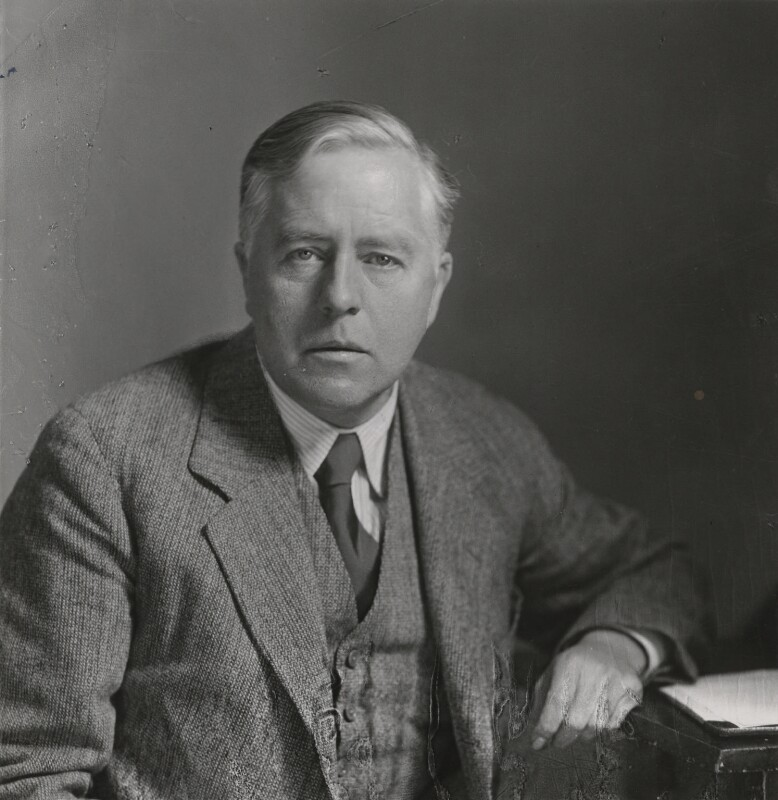
\includegraphics[scale=0.2]{Anh/APho2012.1.jpg}\\
    \textit{James H. Jeans}\\
    $(1877-1946)$
\end{center}
Một nam châm nhỏ có moment lưỡng cực từ $p$ và khối lượng $m$ rơi trong lòng một ống kim loại rất dài, không có từ tính, đặt thẳng đứng, như thấy trong Hình $1$ (hình không vẽ đúng tỉ lệ). Nhìn chung, sự rơi được mô tả bởi phương trình: 
\[m\Ddot{z}=mg-k\Dot{z},\tag{1} \label{i2012.1}\]
với $g$ là gia tốc trọng trường và $k$ gọi là tham số hãm.\\ Sự hãm được gây nên bởi dòng điện xoáy xuất hiện trong ống kim loại. 
\begin{center}
    \tikzset{every picture/.style={line width=0.75pt}} %set default line width to 0.75pt        

\begin{tikzpicture}[x=0.75pt,y=0.75pt,yscale=-1,xscale=1]
%uncomment if require: \path (0,300); %set diagram left start at 0, and has height of 300

%Shape: Ellipse [id:dp6078844013224054] 
\draw   (253.29,60.71) .. controls (253.29,56.01) and (267.62,52.21) .. (285.29,52.21) .. controls (302.97,52.21) and (317.29,56.01) .. (317.29,60.71) .. controls (317.29,65.4) and (302.97,69.21) .. (285.29,69.21) .. controls (267.62,69.21) and (253.29,65.4) .. (253.29,60.71) -- cycle ;
%Shape: Ellipse [id:dp612181013103327] 
\draw   (240.59,60.71) .. controls (240.59,54.15) and (260.6,48.83) .. (285.29,48.83) .. controls (309.98,48.83) and (330,54.15) .. (330,60.71) .. controls (330,67.27) and (309.98,72.58) .. (285.29,72.58) .. controls (260.6,72.58) and (240.59,67.27) .. (240.59,60.71) -- cycle ;
%Straight Lines [id:da6072255552823334] 
\draw    (240.59,59.83) -- (240.59,121.33) ;
%Straight Lines [id:da9762768699823468] 
\draw    (330,60.71) -- (330,121.33) ;
%Straight Lines [id:da33194194901651275] 
\draw  [dash pattern={on 4.5pt off 4.5pt}]  (240.59,121.33) -- (240.59,179.33) ;
%Straight Lines [id:da7387705383182246] 
\draw  [dash pattern={on 4.5pt off 4.5pt}]  (330,121.33) -- (330,179.33) ;
%Straight Lines [id:da07357167794524355] 
\draw    (240.59,179.33) -- (240.59,240.83) ;
%Straight Lines [id:da6030115676990582] 
\draw    (330,179.33) -- (330,240.83) ;
%Curve Lines [id:da6211835397721102] 
\draw    (240.59,240.83) .. controls (241,260.67) and (325,264.67) .. (330,240.83) ;
%Straight Lines [id:da9295985921022609] 
\draw    (209.59,78.83) -- (209.59,137.33) ;
\draw [shift={(209.59,140.33)}, rotate = 270] [fill={rgb, 255:red, 0; green, 0; blue, 0 }  ][line width=0.08]  [draw opacity=0] (10.72,-5.15) -- (0,0) -- (10.72,5.15) -- (7.12,0) -- cycle    ;
%Straight Lines [id:da31637783395092] 
\draw    (361,120.67) -- (305,120.67) ;
\draw [shift={(302,120.67)}, rotate = 360] [fill={rgb, 255:red, 0; green, 0; blue, 0 }  ][line width=0.08]  [draw opacity=0] (10.72,-5.15) -- (0,0) -- (10.72,5.15) -- (7.12,0) -- cycle    ;
%Shape: Rectangle [id:dp13305713828863142] 
\draw  [fill={rgb, 255:red, 21; green, 19; blue, 19 }  ,fill opacity=1 ] (278.51,15.49) -- (278.49,36.49) -- (290.49,36.51) -- (290.51,15.51) -- cycle ;

% Text Node
\draw (190,130.4) node [anchor=north west][inner sep=0.75pt]    {$z$};
% Text Node
\draw (373,113) node [anchor=north west][inner sep=0.75pt]   [align=left] {Ống kim loại};
% Text Node
\draw (301,20) node [anchor=north west][inner sep=0.75pt]   [align=left] {Nam châm};


\end{tikzpicture}\\
Hình $1$.
\end{center}
\begin{enumerate}[1) ]
    \item Xác định vận tốc cuối cùng $(v_{T})$ của nam châm.
    \item Tìm biểu thức $z(t)$, xác định vị trí của nam châm tại thời điểm $t$.\\Lấy $v(t=0)=0$ và $z(t=0)=0$.
\end{enumerate}
Ta sẽ tìm hiểu về động lực học của sự rơi. Muốn vậy, ta xét trong các phần từ $3)$ đến $8)$ một bài toán đơn giản về một nam châm rơi về phía một vòng dây cố định, dọc theo trục của vòng dây. Vòng dây làm bằng kim loại không có từ tính, có bán kính $a$, điện trở $R$ và độ tự cảm $L$ như thấy trên Hình $2$. Trong bài toán này, ta bỏ qua các hiệu ứng bức xạ.\\
\begin{center}
\tikzset{every picture/.style={line width=0.75pt}} %set default line width to 0.75pt        

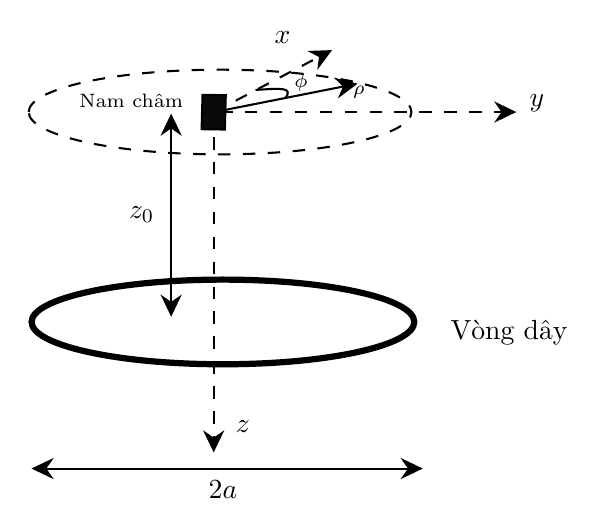
\begin{tikzpicture}[x=0.75pt,y=0.75pt,yscale=-1,xscale=1]
%uncomment if require: \path (0,300); %set diagram left start at 0, and has height of 300

%Shape: Ellipse [id:dp6435461042549706] 
\draw  [line width=2.25]  (211.37,180.79) .. controls (211.37,169.52) and (252.64,160.39) .. (303.56,160.39) .. controls (354.48,160.39) and (395.76,169.52) .. (395.76,180.79) .. controls (395.76,192.05) and (354.48,201.18) .. (303.56,201.18) .. controls (252.64,201.18) and (211.37,192.05) .. (211.37,180.79) -- cycle ;
%Shape: Ellipse [id:dp7400124230045684] 
\draw  [dash pattern={on 4.5pt off 4.5pt}] (210,79.65) .. controls (210,68.38) and (251.28,59.25) .. (302.2,59.25) .. controls (353.11,59.25) and (394.39,68.38) .. (394.39,79.65) .. controls (394.39,90.91) and (353.11,100.04) .. (302.2,100.04) .. controls (251.28,100.04) and (210,90.91) .. (210,79.65) -- cycle ;
%Straight Lines [id:da05547599228687927] 
\draw  [dash pattern={on 4.5pt off 4.5pt}]  (299.12,79.73) -- (299.12,240.66) ;
\draw [shift={(299.12,243.66)}, rotate = 270] [fill={rgb, 255:red, 0; green, 0; blue, 0 }  ][line width=0.08]  [draw opacity=0] (10.72,-5.15) -- (0,0) -- (10.72,5.15) -- (7.12,0) -- cycle    ;
%Straight Lines [id:da5644922579109435] 
\draw  [dash pattern={on 4.5pt off 4.5pt}]  (302.2,79.65) -- (441.93,79.65) ;
\draw [shift={(444.93,79.65)}, rotate = 180] [fill={rgb, 255:red, 0; green, 0; blue, 0 }  ][line width=0.08]  [draw opacity=0] (10.72,-5.15) -- (0,0) -- (10.72,5.15) -- (7.12,0) -- cycle    ;
%Straight Lines [id:da7526895031881755] 
\draw  [dash pattern={on 4.5pt off 4.5pt}]  (299.12,79.73) -- (353.49,51.2) ;
\draw [shift={(356.15,49.81)}, rotate = 512.31] [fill={rgb, 255:red, 0; green, 0; blue, 0 }  ][line width=0.08]  [draw opacity=0] (10.72,-5.15) -- (0,0) -- (10.72,5.15) -- (7.12,0) -- cycle    ;
%Straight Lines [id:da055924410128701085] 
\draw    (299.12,79.73) -- (365.5,66.58) ;
\draw [shift={(368.44,65.99)}, rotate = 528.79] [fill={rgb, 255:red, 0; green, 0; blue, 0 }  ][line width=0.08]  [draw opacity=0] (10.72,-5.15) -- (0,0) -- (10.72,5.15) -- (7.12,0) -- cycle    ;
%Curve Lines [id:da3493574690364205] 
\draw    (319.27,69.03) .. controls (332.93,68.02) and (337.02,68.02) .. (333.78,72.86) ;
%Straight Lines [id:da814025960137122] 
\draw    (278.63,83.41) -- (278.63,175.26) ;
\draw [shift={(278.63,178.26)}, rotate = 270] [fill={rgb, 255:red, 0; green, 0; blue, 0 }  ][line width=0.08]  [draw opacity=0] (10.72,-5.15) -- (0,0) -- (10.72,5.15) -- (7.12,0) -- cycle    ;
\draw [shift={(278.63,80.41)}, rotate = 90] [fill={rgb, 255:red, 0; green, 0; blue, 0 }  ][line width=0.08]  [draw opacity=0] (10.72,-5.15) -- (0,0) -- (10.72,5.15) -- (7.12,0) -- cycle    ;
%Shape: Rectangle [id:dp32200862062183755] 
\draw  [fill={rgb, 255:red, 11; green, 10; blue, 10 }  ,fill opacity=1 ] (304.94,71.54) -- (304.51,88.08) -- (293.3,87.92) -- (293.74,71.38) -- cycle ;
%Straight Lines [id:da05621487384419388] 
\draw [line width=0.75]    (396.85,251.42) -- (214.37,251.42) ;
\draw [shift={(211.37,251.42)}, rotate = 360] [fill={rgb, 255:red, 0; green, 0; blue, 0 }  ][line width=0.08]  [draw opacity=0] (10.72,-5.15) -- (0,0) -- (10.72,5.15) -- (7.12,0) -- cycle    ;
\draw [shift={(399.85,251.42)}, rotate = 180] [fill={rgb, 255:red, 0; green, 0; blue, 0 }  ][line width=0.08]  [draw opacity=0] (10.72,-5.15) -- (0,0) -- (10.72,5.15) -- (7.12,0) -- cycle    ;

% Text Node
\draw (308.37,226.62) node [anchor=north west][inner sep=0.75pt]    {$z$};
% Text Node
\draw (449.85,69.86) node [anchor=north west][inner sep=0.75pt]    {$y$};
% Text Node
\draw (326.93,39.51) node [anchor=north west][inner sep=0.75pt]    {$x$};
% Text Node
\draw (364.8,65.81) node [anchor=north west][inner sep=0.75pt]  [font=\scriptsize]  {$\rho $};
% Text Node
\draw (336.49,59.71) node [anchor=north west][inner sep=0.75pt]  [font=\scriptsize]  {$\phi $};
% Text Node
\draw (411.74,178.69) node [anchor=north west][inner sep=0.75pt]   [align=left] {Vòng dây};
% Text Node
\draw (256.82,123.47) node [anchor=north west][inner sep=0.75pt]    {$z_{0}$};
% Text Node
\draw (232.9,69.41) node [anchor=north west][inner sep=0.75pt]  [font=\scriptsize] [align=left] {Nam châm};
% Text Node
\draw (295.24,255.95) node [anchor=north west][inner sep=0.75pt]    {$2a$};
\end{tikzpicture}\\
Hình $2$.
\end{center}
Trong trường hợp này, sẽ tiện lợi hơn khi dùng hệ tọa độ trụ $(\rho,\varphi,z)$ như trên Hình $2$, trong đó trục $z$ trùng với trục của vòng dây. Ban đầu, nam châm đứng yên ở gốc tọa độ; tâm vòng dây cách gốc tọa độ một khoảng $z_0$. Các trục tọa độ Descartes $(x,y,z)$ cũng được cho trên hình. Nam châm có moment lưỡng cực $\overrightarrow{p}$ hướng theo chiều dương của trục $z$: $\overrightarrow{p}=p\hat{k}$, với $\hat{k}$ là vector đơn vị trên trục $z$. Ta giả thiết rằng trong khi rơi, moment từ của nam châm giữ nguyên hướng. Khi nam châm nằm ở gốc tọa độ, thì từ trường gây bởi nam châm tại một điểm có tọa độ $(\rho,\varphi,z)$ có thành phần dọc trục $(B_{z})$ và thành phần xuyên tâm $(B_{\rho})$ được cho bởi: 
\[\begin{aligned}
    B_{z}&=\dfrac{\mu_0}{4\pi}\dfrac{p}{(\rho^2+z^2)^{\frac{3}{2}}}\left[\dfrac{3z^2}{\rho^2+z^2}-1\right],\\
    B_{\rho}&=\dfrac{\mu_0}{4\pi}\dfrac{3pz\rho}{(\rho^2+z^2)^{\frac{5}{2}}},
\end{aligned}\] 
với $\mu_0$ là độ từ thẩm của chân không.
\begin{enumerate}[1)]
\setcounter{enumi}{2}
    \item Gọi tốc độ tức thời của nam châm là $v$. Hãy xác định độ lớn suất điện động cảm ứng $(e_{i})$ trong vòng dây.
    \item Suất điện động này gây nên dòng cảm ứng $(i)$ trong vòng dây. Hãy xác định độ lớn của lực điện từ tức thời $(f_{\text{em}})$ tác dụng lên vòng dây theo $i$.
    \item Độ lớn của lực mà vòng dây tác dụng lên nam châm bằng bao nhiêu?
    \item Hãy biểu thị suất điện động trong vòng dây theo $L$, $R$ và $i$. Không cần giải để tìm $i$.
    \item Khi nam châm rơi, nó mất dần thế năng trọng trường. Hãy chỉ ra ba dạng chính của năng lượng mà thế năng trọng trường chuyển hóa thành, và viết các công thức sẽ dùng nếu cần tính từng dạng năng lượng đó. 
    \item Trong quá trình này, từ trường của nam châm có thực hiện công hay không?
\end{enumerate}
Tiếp theo, ta ước lượng tham số hãm $k$ cho trường hợp của
ống (xem phương trình (\ref{i2012.1})). Xét ống dài vô hạn, có bán kính $a$, độ dày nhỏ $w$, và độ dẫn diện $\sigma$. Từ phần này trở đi, ta bỏ qua độ tự cảm của ống. Ta xem ống như được tạo thành từ nhiều vòng dây, mỗi vòng dây có độ cao $\Delta z'$, bán kính $a$, độ dày rất mỏng $w$ và độ dẫn điện $\sigma$ (xem Hình $3$). Để đơn giản, ta coi hai đầu ống có tọa độ là $z=-\infty$ và $z=\infty$.
\begin{center}


\tikzset{every picture/.style={line width=0.75pt}} %set default line width to 0.75pt        

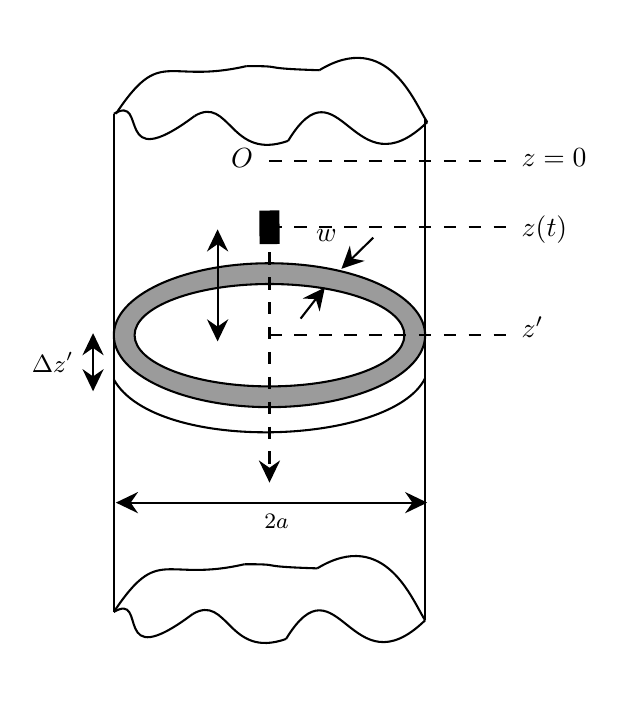
\begin{tikzpicture}[x=0.75pt,y=0.75pt,yscale=-1,xscale=1]
%uncomment if require: \path (0,300); %set diagram left start at 0, and has height of 300

%Shape: Donut [id:dp8312843346003196] 
\draw  [fill={rgb, 255:red, 155; green, 155; blue, 155 }  ,fill opacity=1 ,even odd rule] (191,141.67) .. controls (191,128.04) and (220.1,117) .. (256,117) .. controls (291.9,117) and (321,128.04) .. (321,141.67) .. controls (321,155.29) and (291.9,166.33) .. (256,166.33) .. controls (220.1,166.33) and (191,155.29) .. (191,141.67)(181,141.67) .. controls (181,122.52) and (214.58,107) .. (256,107) .. controls (297.42,107) and (331,122.52) .. (331,141.67) .. controls (331,160.81) and (297.42,176.33) .. (256,176.33) .. controls (214.58,176.33) and (181,160.81) .. (181,141.67) ;
%Straight Lines [id:da8581645335134995] 
\draw    (181,141.67) -- (181,163) ;
%Straight Lines [id:da6296921588002655] 
\draw    (331,141.67) -- (331,162.33) ;
%Curve Lines [id:da8063795216984664] 
\draw    (181,163) .. controls (201,199) and (315,195) .. (331,162.33) ;
%Straight Lines [id:da17318287633113383] 
\draw    (181,35) -- (181,275) ;
%Straight Lines [id:da2233159370082325] 
\draw    (331,37) -- (331,279) ;
%Curve Lines [id:da4730413464853551] 
\draw    (181,275) .. controls (198,265) and (179,306) .. (219,276) ;
%Curve Lines [id:da021373661836334712] 
\draw    (219,276) .. controls (236,266) and (236,298) .. (264,288) ;
%Curve Lines [id:da5117579695710048] 
\draw    (264,288) .. controls (289,247) and (295,314) .. (331,279) ;
%Curve Lines [id:da6518869551809712] 
\draw    (181,275) .. controls (203,242) and (205,261) .. (244,252) ;
%Curve Lines [id:da5342765660730764] 
\draw    (244,252) .. controls (265,252) and (247,253) .. (279,254) ;
%Curve Lines [id:da7817865489186593] 
\draw    (279,254) .. controls (312,234) and (325,270) .. (331,279) ;
%Curve Lines [id:da5263174503814791] 
\draw    (181,35) .. controls (198,25) and (180,66) .. (220,36) ;
%Curve Lines [id:da5268319585625727] 
\draw    (220,36) .. controls (237,26) and (237,58) .. (265,48) ;
%Curve Lines [id:da1930951108450245] 
\draw    (265,48) .. controls (290,7) and (296,74) .. (332,39) ;
%Curve Lines [id:da9788816334466668] 
\draw    (182,35) .. controls (204,2) and (206,21) .. (245,12) ;
%Curve Lines [id:da7323244141892633] 
\draw    (245,12) .. controls (266,12) and (248,13) .. (280,14) ;
%Curve Lines [id:da2315376376069218] 
\draw    (280,14) .. controls (313,-6) and (326,30) .. (332,39) ;
%Straight Lines [id:da1506838382572886] 
\draw    (185,222.33) -- (329,222.33) ;
\draw [shift={(332,222.33)}, rotate = 180] [fill={rgb, 255:red, 0; green, 0; blue, 0 }  ][line width=0.08]  [draw opacity=0] (10.72,-5.15) -- (0,0) -- (10.72,5.15) -- (7.12,0) -- cycle    ;
\draw [shift={(182,222.33)}, rotate = 0] [fill={rgb, 255:red, 0; green, 0; blue, 0 }  ][line width=0.08]  [draw opacity=0] (10.72,-5.15) -- (0,0) -- (10.72,5.15) -- (7.12,0) -- cycle    ;
%Straight Lines [id:da8700643223831148] 
\draw  [dash pattern={on 4.5pt off 4.5pt}]  (256,89.67) -- (256,209.67) ;
\draw [shift={(256,212.67)}, rotate = 270] [fill={rgb, 255:red, 0; green, 0; blue, 0 }  ][line width=0.08]  [draw opacity=0] (10.72,-5.15) -- (0,0) -- (10.72,5.15) -- (7.12,0) -- cycle    ;
%Straight Lines [id:da9280090267594727] 
\draw    (231,93.67) -- (231,141.67) ;
\draw [shift={(231,144.67)}, rotate = 270] [fill={rgb, 255:red, 0; green, 0; blue, 0 }  ][line width=0.08]  [draw opacity=0] (10.72,-5.15) -- (0,0) -- (10.72,5.15) -- (7.12,0) -- cycle    ;
\draw [shift={(231,90.67)}, rotate = 90] [fill={rgb, 255:red, 0; green, 0; blue, 0 }  ][line width=0.08]  [draw opacity=0] (10.72,-5.15) -- (0,0) -- (10.72,5.15) -- (7.12,0) -- cycle    ;
%Straight Lines [id:da6605418042753075] 
\draw  [dash pattern={on 4.5pt off 4.5pt}]  (256,141.67) -- (370,141.67) ;
%Straight Lines [id:da4115042756618199] 
\draw  [dash pattern={on 4.5pt off 4.5pt}]  (256,89.67) -- (370,89.67) ;
%Straight Lines [id:da31516998020231557] 
\draw  [dash pattern={on 4.5pt off 4.5pt}]  (256,57.67) -- (370,57.67) ;
%Shape: Rectangle [id:dp9504791545129123] 
\draw  [fill={rgb, 255:red, 0; green, 0; blue, 0 }  ,fill opacity=1 ] (260.29,82.06) -- (260.38,97.22) -- (251.71,97.28) -- (251.62,82.11) -- cycle ;
%Straight Lines [id:da16857508513893782] 
\draw    (171,143.67) -- (171,165.67) ;
\draw [shift={(171,168.67)}, rotate = 270] [fill={rgb, 255:red, 0; green, 0; blue, 0 }  ][line width=0.08]  [draw opacity=0] (10.72,-5.15) -- (0,0) -- (10.72,5.15) -- (7.12,0) -- cycle    ;
\draw [shift={(171,140.67)}, rotate = 90] [fill={rgb, 255:red, 0; green, 0; blue, 0 }  ][line width=0.08]  [draw opacity=0] (10.72,-5.15) -- (0,0) -- (10.72,5.15) -- (7.12,0) -- cycle    ;
%Straight Lines [id:da3339036824847832] 
\draw    (271,133.67) -- (280.82,121.03) ;
\draw [shift={(282.67,118.67)}, rotate = 487.87] [fill={rgb, 255:red, 0; green, 0; blue, 0 }  ][line width=0.08]  [draw opacity=0] (10.72,-5.15) -- (0,0) -- (10.72,5.15) -- (7.12,0) -- cycle    ;
%Straight Lines [id:da17139286844650492] 
\draw    (306,94.67) -- (292.81,107.57) ;
\draw [shift={(290.67,109.67)}, rotate = 315.63] [fill={rgb, 255:red, 0; green, 0; blue, 0 }  ][line width=0.08]  [draw opacity=0] (10.72,-5.15) -- (0,0) -- (10.72,5.15) -- (7.12,0) -- cycle    ;

% Text Node
\draw (252,226.4) node [anchor=north west][inner sep=0.75pt]  [font=\footnotesize]  {$2a$};
% Text Node
\draw (236,50.4) node [anchor=north west][inner sep=0.75pt]    {$O$};
% Text Node
\draw (376,50.4) node [anchor=north west][inner sep=0.75pt]    {$z=0$};
% Text Node
\draw (376,82.4) node [anchor=north west][inner sep=0.75pt]    {$z( t)$};
% Text Node
\draw (376,131.4) node [anchor=north west][inner sep=0.75pt]    {$z'$};
% Text Node
\draw (140,148.4) node [anchor=north west][inner sep=0.75pt]  [font=\small]  {$\Delta z'$};
% Text Node
\draw (277,89.4) node [anchor=north west][inner sep=0.75pt]    {$w$};


\end{tikzpicture}\\
Hình $3$.
\end{center}
\begin{enumerate}[1) ]
\setcounter{enumi}{8}
    \item Tìm điện trở của mỗi vòng dây đó.
    \item Tìm tham số hãm $k$  gây nên bởi toàn bộ ống theo $p$, $\sigma$ và các tham số hình học của vòng dây. Vì rằng thành ống rất mỏng, nên có thể coi rằng từ trường là như nhau trong toàn bộ bề dày của vòng và bằng $B_{\rho}(\rho=a)$. Giả thiết rằng ở thời điểm $t$, nam châm có toạ độ $z(t)$ và có tốc độ tức thời $\Dot{z}$. Viết kết quả dưới dạng một biểu thức có chứa tích phân $I$, theo biến không thứ nguyên $u=\dfrac{(z-z')}{a}$.
    \item Giả sử tham số hãm $k$ là hàm số:
    \[k=f(\mu_0, p, R_0, a),\]
    với $R_0$ là điện trở hiệu dụng của ống. Bằng cách sử dụng phép phân tích thứ nguyên, hãy tìm biểu thức của $k$. Lấy hệ số tỉ lệ không thứ nguyên bằng đơn vị.
\end{enumerate}
\begin{center}
    \bf Tích phân sau có thể được sử dụng:
\end{center}
\[\int \dfrac{u\mathrm{d}u}{(u^2+a^2)^{n}}=\dfrac{1}{2}\dfrac{(a^2+u^2)^{1-n}}{1-n}+\text{Hằng số}~(\text{với}~n>1).\]
\textbf{Chú ý.} $\Dot{z}=\dfrac{\mathrm{d}z}{\mathrm{d}t}$; $\Ddot{z}=\dfrac{\mathrm{d}^2z}{\mathrm{d}t^2}$.
\end{vd}
\begin{loigiai} 
\begin{enumerate}[1)]
    \item Tìm vận tốc cuối $(v_{T})$ của nam châm.\\
Phương trình chuyển động của nam châm là:
\[m\Ddot{z}=mg-k\Dot{z}. \tag{1} \label{apho12sa.1}\]
Đối với vận tốc cuối, $\Ddot{z}=0$. Từ đó suy ra:
\[v_{T}=\Dot{z}=\dfrac{mg}{k}. \tag{2} \label{apho12sa.2}\]
    \item Tìm vị trí $z(t)$ của nam châm tại thời điểm $t$.\\
    Viết lại phương trình (\ref{apho12sa.1}) dưới dạng
    \[\dfrac{\mathrm{d}v}{\mathrm{d}t}=g-\dfrac{k}{m}v(t). \tag{3} \label{apho12sa.3}\]
    Ta giải phương trình (\ref{apho12sa.3}) với điều kiện ban đầu $v(t=0)=0$; $z(t=0)=0$. Kết quả là:
    \[v(t)=\dfrac{mg}{k}(1-e^{-kt/m})=\dfrac{\mathrm{d}z}{\mathrm{d}t}, \tag{4} \label{apho12sa.4}\]
    \[\int_0^z\mathrm{d}z=\int_0^t\dfrac{mg}{k}(1-e^{-kt/m})\mathrm{d}t~,~z(t)=\dfrac{mg}{k}\left[t+\dfrac{m}{k}(e^{-kt/m}-1)\right]. \tag{5} \label{apho12sa.5}\]
    \item Tính độ lớn suất điện động cảm ứng $(e_{i})$ trong vòng.\\
    Cách thứ nhất là sử dụng vận tốc tương đối $v$ giữa nam châm và vòng trong từ trường $\overrightarrow{B}=B_{k}\overrightarrow{k}+B_{\rho}\overrightarrow{\rho}$ của nam châm, từ đó tính được suất điện động cảm ứng:
    \[e_{i}=\int\left[\overrightarrow{v}\wedge\overrightarrow{B}\right]\mathrm{d}\overrightarrow{\ell}=vB_{a}\cdot2\pi a~,~B_{a}=\dfrac{\mu_0}{4\pi}\dfrac{3pa(z_0-z)}{\left[a^2+(z_0-z)^2\right]^{5/2}}. \tag{6} \label{apho12sa.6}\]
    Cách thứ hai là xét từ thông $\phi$ qua vòng: 
    
    \begin{align*}
     \phi&=\int_0^aB_{z}2\pi\rho\mathrm{d}\rho=2\pi\int_0^a\dfrac{\mu_0}{4\pi}\dfrac{\rho p}{[\rho^2+(z_0-z)^2]^{3/2}}\left[\dfrac{3(z_0-z)^2}{\rho^2+(z_0-z)^2}-1\right]\mathrm{d}\rho\\
    &=\dfrac{\mu_0pa^2}{2[a^2+(z_0-z)^2]^{3/2}}. \tag{7} \label{apho12sa.7}
    \end{align*}
    
    Từ đó, suy ra
    \[e_{i}=\dfrac{-\mathrm{d}\phi}{\mathrm{d}t}=-v\dfrac{\mathrm{d}\phi}{\mathrm{z}}~\Rightarrow e_{i}=\dfrac{\mu_03pa^2v(z_0-z)}{2[a^2+(z_0-z)^2]^{5/2}}. \tag{8} \label{apho12sa.8}\]
    \item Tính lực điện từ tức thời $(f_{\text{em}})$ tác dụng lên vòng theo $i$.\\
    Thành phần $B_{z}$ sẽ gây ra lực xuyên tâm hướng ra bên ngoài trên vòng và do đối xứng dẫn tới một lực bằng không.\\
    Chỉ thành phần $B_{\rho}$ có đóng góp:
    
    \[\mathrm{d}\overrightarrow{f_{\text{em}}}=i\left[\mathrm{d}\overrightarrow{\ell}\wedge\overrightarrow{B}\right]~\Rightarrow \left|\overrightarrow{f_{\text{em}}}\right|=i2\pi aB_{a}, \tag{9} \label{apho12sa.9}\]
    ở đây $B_{a}$ được cho bởi biểu thức (\ref{apho12sa.6}).
    \item Tính độ lớn lực của vòng tác dụng lên nam châm.\\
    Theo định luật III Newton, tồn tại một lực trực đối của lực $\overrightarrow{f_{\text{em}}}$ do vòng tác dụng lên nam châm. Do đó, độ lớn lực của vòng tác dụng lên nam châm là $f_{\text{em}}$.
    \item Biểu diễn suất điện động trong vòng theo $L$, $R$ và $i$.\\
    Kết quả là:
    \[e_{i}=L\dfrac{\mathrm{d}i}{\mathrm{d}t}+R. \tag{10 \label{apho12sa.10}}\]
    \item Xác định ba dạng năng lượng chính mà thế năng hấp dẫn chuyển đổi thành chúng và viết các biểu thức cho ba dạng này.\\
    Thế năng chuyển đổi thành ba phần là
\[ \dfrac{mv^2}{2}~~(\text{động năng}),\tag{11} \label{apho12sa.11}\]
\[\dfrac{Li^2}{2}~~(\text{năng lượng từ trường}), \tag{12} \label{apho12sa.12}\]
\[i^2R\Delta t~~(\text{sự mất mát nhiệt năng Joule do dòng điện trong thời gian $\Delta t$}). \tag{13} \label{apho12sa.13}\]

    \item Từ trường của nam châm có sinh công trong quá trình này không?\\ Câu trả lời là không.
    \item Tính điện trở của vòng.\\
    \[\Delta R=\dfrac{2\pi a}{\sigma \omega \Delta z'}. \tag{14} \label{apho12sa.14}\]
    \item Tính thông số tắt dần $k$ gây nên bởi toàn bộ ống theo $p$, $\sigma$ và các thông số hình học của vòng.\\
    Hợp lực lên nam châm do một vòng tại $z'$ được cho bởi
    \begin{align*}
        f_{\text{em}}&=(2\pi a)iB'_{a}, \tag{15} \label{apho12sa.15}\\
        B'_{a}&=\dfrac{\mu_0}{4\pi}\dfrac{3pa(z'-z)}{[a^2+(z'-z)^2]^{5/2}}, \tag{16} \label{apho12sa.16}\\
        i&=\dfrac{h}{\Delta R}=\dfrac{\sigma we_{i}}{2\pi a}\Delta z', \tag{17} \label{apho12sa.17}
    \end{align*}
    
    trong đó, $i$ là dòng điện cảm ứng trong vòng.\\
    Hợp lực tác dụng lên nam châm do toàn bộ ống là:
    
    \[F=\int_{-\infty}^\infty f_{em}=\int_{-\infty}^\infty B'^2_{a}(2\pi a)w\sigma\dd z'\cdot\Dot{z}.\]
    
    Do ống rất dài nên có thể lấy tích phân từ $-\infty$ đến $\infty$. Khi thay thế $B'_{a}$, ta có:
    
    \[F=\left(\dfrac{\mu_0}{4\pi}\right)^2\cdot18p^2a^3\pi w\sigma \Dot{z}\int_{-\infty}^\infty \dfrac{(z'-z)^2}{[(z'-z)^2+a^2]^5}\mathrm{d}z'.\]
    
    Đặt $u=\dfrac{z'-z}{a}$, cuối cùng ta có:
    
    \[F=\left(\dfrac{\mu_0}{4\pi}\right)^2\dfrac{18p^2\pi w\sigma\Dot{z}}{a^5}\int_{-\infty}^\infty\dfrac{u^2}{(1+u^2)^5}\mathrm{d}u. \tag{18} \label{apho12sa.18} \]
    
    Thông số tắt dần được xác định bởi:
    
    \[k=\dfrac{F}{\Dot{z}}=\left(\dfrac{\mu_0}{4\pi}\right)^2\dfrac{18p^2\pi w\sigma}{a^5}\int_{-\infty}^\infty\dfrac{u^2}{(1+u^2)^5}\mathrm{d}u. \tag{19} \label{apho12sa.19}\]
    
    \item Sử dụng phép tích phân thứ nguyên để tìm biểu thức của $k$.\\
    Cho $k=f(\mu_0,p,R_0,a)$.\\
    Các thứ nguyên của các thông số ống bao hàm là
    \[[\mu_0]=\mathrm{I^{-2}MLT^{-2}}, \tag{20 \label{apho12sa.20}}\]
    \[[p]=\mathrm{IL^2}, \tag{21} \label{apho12sa.21}\]
    \[[R_0]=\mathrm{I^{-2}ML^2T^{-3}}, \tag{22} \label{apho12sa.22}\]
    \[[a]=\mathrm{L}, \tag{23} \label{apho12sa.23}\]
    \[k=\mathrm{MT^{-1}}. \tag{24} \label{apho12sa.24}\]
    Từ đó suy ra:
    \[k=\dfrac{p^2\mu_0^2}{a^4R_0}. \tag{25} \label{apho12sa.25}\]
\end{enumerate}
\end{loigiai}


\begin{vd}[Tụ điện trong chất lỏng dẫn điện]
%Tonghop %APhO 2013 (Indonesia)
Một hệ gồm hai vật dẫn được nhúng chìm trong một chất điện môi lỏng đồng chất, dẫn điện kém. Khi một hiệu điện thế không đổi được đặt vào giữa hai vật dẫn, thì hệ có cả điện trường và từ
trường. Trong bài toán này, ta sẽ khảo sát một hệ như vậy.
\begin{enumerate}[1)]
    \item Đầu tiên, xét một dây dài vô hạn, đặt trong chân không, với điện tích trên một đơn vị chiều dài là $\lambda$. Tính cường độ điện trường \textbf{$E(r)$} do dây gây ra.
    \item Điện thế gây bởi dây dài tích điện có thể được viết dưới dạng 
    \[V(r)=f(r)+K,\]
    trong đó, $K$ là hằng số. Hãy xác định $f(r)$.
    \item Hãy tính điện thế trong toàn không gian $V(x,y,z)$ được gây nên một dây dài vô hạn với điện tích trên một đơn vị chiều dài là $\lambda$, đặt tại $x=-b$ và một dây dài vô hạn khác với điện tích trên một đơn vị chiều dài là $-\lambda$, đặt tại $x=b$. Cả hai dây đều song song với trục $z$. Lấy $V=0$ tại gốc tọa độ.\\
    Hãy phác họa các mặt đẳng thế.
\end{enumerate}
\begin{center}
        Đối với các câu hỏi sau đây, bỏ qua mọi hiệu ứng rìa.
\end{center}
\begin{enumerate}[1)]
\setcounter{enumi}{3}
    \item Bây giờ, xét hai vật dẫn hình trụ rỗng giống nhau, có bán kính $R=3a$, đặt trong chân không. Độ dài của hai vật bằng nhau và lớn hơn nhiều so với bán kính của vật $l\gg R$. Các trục của cả hai vật đều thuộc mặt phẳng $xz$ và song song với trục $z$, một trục cắt trục $x$ tại $x=-5a$ và trục kia cắt trục $x$ tại $x=5a$. Một hiệu điện thế $V_0$ được đặt vào giữa hai vật (vật ở $x=-5a$ có điện thế cao hơn) bằng cách mắc chúng vào một bộ pin. Tính điện thế trong tất cả các miền không gian. Lấy $V=0$ tại gốc tọa độ.
    \item Tính điện dung $C$ của hệ.
    \item Bây giờ nhúng cả hai vật dẫn hình trụ trong một chất lỏng dẫn điện kém, với độ dẫn điện là $\sigma$. Hãy tính dòng điện toàn phần chạy giữa hai vật này. Giả sử hằng số điện môi của chất lỏng bằng hằng số điện môi của của chân không, $\varepsilon=\varepsilon_0$.
    \item Tính điện trở $R$ và tích $RC$ của hệ hai vật hình trụ.
    \item Hãy xác định từ trường của dòng điện được đề cập trong ý $6$. Cho rằng độ từ thẩm của chất lỏng bằng độ từ thẩm của chân không $\mu=\mu_0$.
\end{enumerate}
\textit{Cho tích phân:} $\di\int\dfrac{a\mathrm{d}x}{a^2+x^2}=\arctan{\dfrac{x}{a}}+\text{hằng số}$.
\end{vd}
\begin{loigiai}
\begin{enumerate}[1)]
    \item Tính điện trường $\overrightarrow{E}\tron{\overrightarrow{r}}$.\\
    Áp dụng định luật Gauss:
    \[\oint E \cdot \mathrm{d}A=\dfrac{q}{\varepsilon_0}. \tag{1} \label{apho13sa.1}\]
    Do tính chất đối xứng, điện trường chỉ có thành phần xuyên tâm. Chọn mặt Gauss là mặt trụ có trục đối xứng trùng với dây, ta thu được:
    \[E.2\pi r\ell=\dfrac{\lambda\ell}{\varepsilon_0}.\]
    Từ đó,
    \[\overrightarrow{E}=\dfrac{\lambda}{2\pi\varepsilon_0}\dfrac{\overrightarrow{r}}{r}. \tag{2} \label{apho13sa.2}\]
    \item Xác định $f(r)$.\\
    Điện thế được cho bởi
    \begin{align*}
        V&=-\int_{\text{ref}}^{r}\overrightarrow{E}\mathrm{d}\overrightarrow{\ell}=-\int_{\text{ref}}^{r}E\mathrm{d}r=-\dfrac{\lambda}{2\pi\varepsilon_0}\ln{r}+K=f(r)+K,\\
        f(r)&=-\dfrac{\lambda}{2\pi\varepsilon_0}\ln{r},~ K= \const. \tag{3} \label{apho13sa.3}
    \end{align*}
    \item Tính điện thế $V(x,y,z)$. Phác họa các bề mặt đẳng thế.\\
    Thế năng do cả hai dây mang điện tích là một sự chồng chất thế năng từ mỗi dây.
    \begin{center}
\tikzset{every picture/.style={line width=0.75pt}} %set default line width to 0.75pt        

\begin{tikzpicture}[x=0.75pt,y=0.75pt,yscale=-1,xscale=1]
%uncomment if require: \path (0,300); %set diagram left start at 0, and has height of 300

%Straight Lines [id:da20586263790663417] 
\draw    (110,190.67) -- (422,190.67) ;
\draw [shift={(425,190.67)}, rotate = 180] [fill={rgb, 255:red, 0; green, 0; blue, 0 }  ][line width=0.08]  [draw opacity=0] (10.72,-5.15) -- (0,0) -- (10.72,5.15) -- (7.12,0) -- cycle    ;
%Straight Lines [id:da3593402025789645] 
\draw    (270,210.33) -- (270,45.33) ;
\draw [shift={(270,42.33)}, rotate = 450] [fill={rgb, 255:red, 0; green, 0; blue, 0 }  ][line width=0.08]  [draw opacity=0] (10.72,-5.15) -- (0,0) -- (10.72,5.15) -- (7.12,0) -- cycle    ;
%Straight Lines [id:da6178338081679633] 
\draw  [dash pattern={on 0.84pt off 2.51pt}]  (310,100.33) -- (350,190.67) ;
%Straight Lines [id:da04646592881569167] 
\draw  [dash pattern={on 0.84pt off 2.51pt}]  (310,100.33) -- (190,190.67) ;

% Text Node
\draw (175,191.4) node [anchor=north west][inner sep=0.75pt]    {$-b$};
% Text Node
\draw (345,191.4) node [anchor=north west][inner sep=0.75pt]    {$b$};
% Text Node
\draw (182,170.4) node [anchor=north west][inner sep=0.75pt]    {$\lambda $};
% Text Node
\draw (316,171.4) node [anchor=north west][inner sep=0.75pt]    {$-\lambda $};
% Text Node
\draw (218,140.4) node [anchor=north west][inner sep=0.75pt]    {$r_{1}$};
% Text Node
\draw (334,127.4) node [anchor=north west][inner sep=0.75pt]    {$r_{2}$};
% Text Node
\draw (250,54.4) node [anchor=north west][inner sep=0.75pt]    {$y$};
% Text Node
\draw (408,196.4) node [anchor=north west][inner sep=0.75pt]    {$x$};


\end{tikzpicture}

    \end{center}
    \begin{center}
        \textbf{Hình 1.} Hệ với hai dây dẫn tích điện đều.
    \end{center}
    \[V=-\dfrac{\lambda}{2\pi\varepsilon_0}\ln{r_1}+\dfrac{\lambda}{2\pi\varepsilon_0}\ln{r_2}=\dfrac{\lambda}{2\pi\varepsilon_0}\ln{\dfrac{\sqrt{(b-x)^2+y^2}}{\sqrt{(b+x)^2+y^2}}}. \tag{4} \label{apho13sa.4}\]
    \[\rt V=\dfrac{\lambda}{4\pi\varepsilon_0}\ln{\dfrac{(b-x)^2+y^2}{(b+x)^2+y^2}}. \tag{5} \label{apho13sa.5}\] 
    Ta có thể biến đổi biểu thức (\ref{apho13sa.5}) thành
    \[\left[x-\left(\dfrac{1+\beta}{1-\beta}\right)\right]^2+y^2=b^2\left[\left(\dfrac{1+\beta}{1-\beta}\right)^2-1\right], \tag{6} \label{apho13sa.6}\]
    trong đó,
    \[\beta=\exp{\left(\dfrac{4\pi\varepsilon_0V}{\lambda}\right)}.\]
    Đối với một điện thế $V$ tùy ý, (\ref{apho13sa.6}) là phương trình của đường tròn (Hình $2$).
    \begin{center}
        \tikzset{every picture/.style={line width=0.75pt}} %set default line width to 0.75pt       
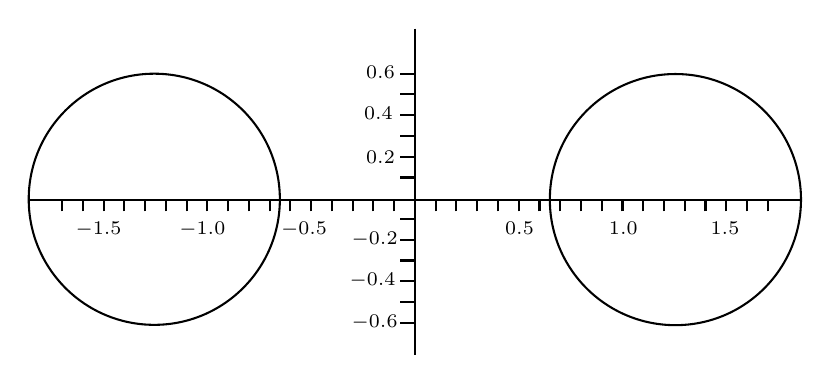
\begin{tikzpicture}[x=0.75pt,y=0.75pt,yscale=-1,xscale=1]
%uncomment if require: \path (0,300); %set diagram left start at 0, and has height of 300

%Straight Lines [id:da10693543426460783] 
\draw    (143.92,157.33) -- (516,157.33) ;
%Straight Lines [id:da3103146478005012] 
\draw    (330,75) -- (330,232) ;
%Straight Lines [id:da8245176705593462] 
\draw    (320,163) -- (320,157.67) ;
%Straight Lines [id:da3869717118569522] 
\draw    (310,163) -- (310,157.67) ;
%Straight Lines [id:da2896364900057129] 
\draw    (300,163) -- (300,157.67) ;
%Straight Lines [id:da9732287898962051] 
\draw    (290,163) -- (290,157.67) ;
%Straight Lines [id:da26173531264308303] 
\draw    (280,163) -- (280,157.67) ;
%Straight Lines [id:da5060456076916551] 
\draw    (270,163) -- (270,157.67) ;
%Straight Lines [id:da3158583130304451] 
\draw    (260,163) -- (260,157.67) ;
%Straight Lines [id:da8463799999955766] 
\draw    (250,163) -- (250,157.67) ;
%Straight Lines [id:da9360396153356727] 
\draw    (240,163) -- (240,157.67) ;
%Straight Lines [id:da09586038418322018] 
\draw    (230,163) -- (230,157.67) ;
%Straight Lines [id:da5042715623231964] 
\draw    (220,163) -- (220,157.67) ;
%Straight Lines [id:da4079413348575096] 
\draw    (210,163) -- (210,157.67) ;
%Straight Lines [id:da30770166578596214] 
\draw    (200,163) -- (200,157.67) ;
%Straight Lines [id:da7271762623048859] 
\draw    (190,163) -- (190,157.67) ;
%Straight Lines [id:da6584649516678565] 
\draw    (180,163) -- (180,157.67) ;
%Straight Lines [id:da16719188934813545] 
\draw    (340,163) -- (340,157.67) ;
%Straight Lines [id:da531651144043664] 
\draw    (350,163) -- (350,157.67) ;
%Straight Lines [id:da5867417104959234] 
\draw    (360,163) -- (360,157.67) ;
%Straight Lines [id:da3384814600145336] 
\draw    (370,163) -- (370,157.67) ;
%Straight Lines [id:da8745480922226434] 
\draw    (380,163) -- (380,157.67) ;
%Straight Lines [id:da36491940365480646] 
\draw    (390,163) -- (390,157.67) ;
%Straight Lines [id:da46039068295306973] 
\draw    (400,163) -- (400,157.67) ;
%Straight Lines [id:da9241442401613649] 
\draw    (410,163) -- (410,157.67) ;
%Straight Lines [id:da9724842765070336] 
\draw    (420,163) -- (420,157.67) ;
%Straight Lines [id:da38963657239082505] 
\draw    (430,163) -- (430,157.67) ;
%Straight Lines [id:da1745812557539137] 
\draw    (440,163) -- (440,157.67) ;
%Straight Lines [id:da8640331710903635] 
\draw    (460,163) -- (460,157.67) ;
%Straight Lines [id:da6566384255876303] 
\draw    (480,163) -- (480,157.67) ;
%Straight Lines [id:da06493751970941641] 
\draw    (470,163) -- (470,157.67) ;
%Straight Lines [id:da3571172821878006] 
\draw    (450,163) -- (450,157.67) ;
%Straight Lines [id:da868103216314138] 
\draw    (490,163) -- (490,157.67) ;
%Straight Lines [id:da9153496543950912] 
\draw    (500,163) -- (500,157.67) ;
%Straight Lines [id:da6974442633290248] 
\draw    (330,176.67) -- (323,176.67) ;
%Straight Lines [id:da9858239463086906] 
\draw    (330,196.67) -- (323,196.67) ;
%Straight Lines [id:da6619642859497705] 
\draw    (330,216.67) -- (323,216.67) ;
%Straight Lines [id:da6219377266823873] 
\draw    (330,206.67) -- (323,206.67) ;
%Straight Lines [id:da3599949378577316] 
\draw    (330,186.67) -- (323,186.67) ;
%Straight Lines [id:da7038808423931626] 
\draw    (330,166.67) -- (323,166.67) ;
%Straight Lines [id:da8184073239580727] 
\draw    (330,146.67) -- (323,146.67) ;
%Straight Lines [id:da2400184091007329] 
\draw    (330,136.67) -- (323,136.67) ;
%Straight Lines [id:da9852506000532384] 
\draw    (330,126.67) -- (323,126.67) ;
%Straight Lines [id:da6360794769693767] 
\draw    (330,116.67) -- (323,116.67) ;
%Straight Lines [id:da20505254462663491] 
\draw    (330,106.67) -- (323,106.67) ;
%Straight Lines [id:da6801966692025674] 
\draw    (330,96.67) -- (323,96.67) ;
%Shape: Circle [id:dp5196243670531799] 
\draw   (143.92,157.17) .. controls (143.92,123.75) and (171,96.67) .. (204.42,96.67) .. controls (237.83,96.67) and (264.92,123.75) .. (264.92,157.17) .. controls (264.92,190.58) and (237.83,217.67) .. (204.42,217.67) .. controls (171,217.67) and (143.92,190.58) .. (143.92,157.17) -- cycle ;
%Shape: Circle [id:dp5511881887177501] 
\draw   (395,157.33) .. controls (395,123.92) and (422.09,96.83) .. (455.5,96.83) .. controls (488.91,96.83) and (516,123.92) .. (516,157.33) .. controls (516,190.75) and (488.91,217.83) .. (455.5,217.83) .. controls (422.09,217.83) and (395,190.75) .. (395,157.33) -- cycle ;

%Straight Lines [id:da7093919674906228] 
\draw    (170,163) -- (170,157.67) ;
%Straight Lines [id:da9917455866724287] 
\draw    (160,163) -- (160,157.67) ;


% Text Node
\draw (372,166.4) node [anchor=north west][inner sep=0.75pt]  [font=\scriptsize]  {$0.5$};
% Text Node
\draw (422,166.4) node [anchor=north west][inner sep=0.75pt]  [font=\scriptsize]  {$1.0$};
% Text Node
\draw (471,166.4) node [anchor=north west][inner sep=0.75pt]  [font=\scriptsize]  {$1.5$};
% Text Node
\draw (264,166.4) node [anchor=north west][inner sep=0.75pt]  [font=\scriptsize]  {$-0.5$};
% Text Node
\draw (215,166.4) node [anchor=north west][inner sep=0.75pt]  [font=\scriptsize]  {$-1.0$};
% Text Node
\draw (165,166.4) node [anchor=north west][inner sep=0.75pt]  [font=\scriptsize]  {$-1.5$};
% Text Node
\draw (305,132.4) node [anchor=north west][inner sep=0.75pt]  [font=\scriptsize]  {$0.2$};
% Text Node
\draw (304,111.4) node [anchor=north west][inner sep=0.75pt]  [font=\scriptsize]  {$0.4$};
% Text Node
\draw (305,91.4) node [anchor=north west][inner sep=0.75pt]  [font=\scriptsize]  {$0.6$};
% Text Node
\draw (298,171.4) node [anchor=north west][inner sep=0.75pt]  [font=\scriptsize]  {$-0.2$};
% Text Node
\draw (297,191.4) node [anchor=north west][inner sep=0.75pt]  [font=\scriptsize]  {$-0.4$};
% Text Node
\draw (298,211.4) node [anchor=north west][inner sep=0.75pt]  [font=\scriptsize]  {$-0.6$};


\end{tikzpicture}
    \end{center}
    \begin{center}
        \textbf{Hình 2.} Các mặt đẳng thế với $b=1$ đối với\\ $\beta=12.35$ (bên trái) và $\beta=\dfrac{1}{12.35}$ (bên phải).
    \end{center}
    \item Tính điện thế trong tất cả các vùng.\\
    Từ các phương trình (\ref{apho13sa.5}) và (\ref{apho13sa.6}) ta thấy rằng đối với bất kì giá trị nào của điện thế $V$, mặt đẳng thế của hai dây dẫn (mật độ điện tích dài có độ lớn bằng nhau nhưng trái dấu) là một mặt trụ. Do đó, ta có thể chọn vị trí cụ thể cho mỗi dây để mặt của trụ đều là mặt đẳng thế.\\
    Xét Hình $3$
    \begin{center}


\tikzset{every picture/.style={line width=0.75pt}} %set default line width to 0.75pt        

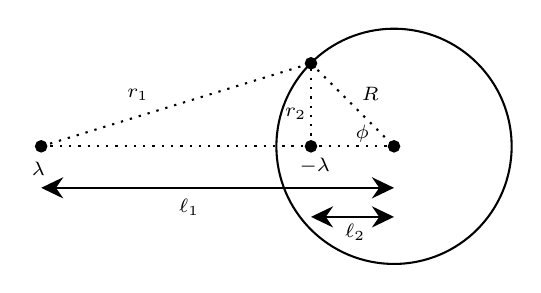
\begin{tikzpicture}[x=0.75pt,y=0.75pt,yscale=-1,xscale=1]
%uncomment if require: \path (0,300); %set diagram left start at 0, and has height of 300

%Shape: Circle [id:dp5630232295971143] 
\draw   (333.33,170.33) .. controls (333.33,139.04) and (358.7,113.67) .. (390,113.67) .. controls (421.3,113.67) and (446.67,139.04) .. (446.67,170.33) .. controls (446.67,201.63) and (421.3,227) .. (390,227) .. controls (358.7,227) and (333.33,201.63) .. (333.33,170.33) -- cycle ;
%Straight Lines [id:da41879549813935446] 
\draw  [dash pattern={on 0.84pt off 2.51pt}]  (220,170.33) -- (390,170.33) ;
%Straight Lines [id:da4682878912238828] 
\draw  [dash pattern={on 0.84pt off 2.51pt}]  (220,170.33) -- (350,130.33) ;
%Straight Lines [id:da8267906678358548] 
\draw  [dash pattern={on 0.84pt off 2.51pt}]  (350,130.33) -- (390,170.33) ;
%Shape: Circle [id:dp7827821281625822] 
\draw  [fill={rgb, 255:red, 0; green, 0; blue, 0 }  ,fill opacity=1 ] (217.5,170.33) .. controls (217.5,168.95) and (218.62,167.83) .. (220,167.83) .. controls (221.38,167.83) and (222.5,168.95) .. (222.5,170.33) .. controls (222.5,171.71) and (221.38,172.83) .. (220,172.83) .. controls (218.62,172.83) and (217.5,171.71) .. (217.5,170.33) -- cycle ;
%Shape: Circle [id:dp613385859313351] 
\draw  [fill={rgb, 255:red, 0; green, 0; blue, 0 }  ,fill opacity=1 ] (347.5,170.33) .. controls (347.5,168.95) and (348.62,167.83) .. (350,167.83) .. controls (351.38,167.83) and (352.5,168.95) .. (352.5,170.33) .. controls (352.5,171.71) and (351.38,172.83) .. (350,172.83) .. controls (348.62,172.83) and (347.5,171.71) .. (347.5,170.33) -- cycle ;
%Shape: Circle [id:dp8284054405248202] 
\draw  [fill={rgb, 255:red, 0; green, 0; blue, 0 }  ,fill opacity=1 ] (387.5,170.33) .. controls (387.5,168.95) and (388.62,167.83) .. (390,167.83) .. controls (391.38,167.83) and (392.5,168.95) .. (392.5,170.33) .. controls (392.5,171.71) and (391.38,172.83) .. (390,172.83) .. controls (388.62,172.83) and (387.5,171.71) .. (387.5,170.33) -- cycle ;
%Shape: Circle [id:dp9133408818236997] 
\draw  [fill={rgb, 255:red, 0; green, 0; blue, 0 }  ,fill opacity=1 ] (347.5,130.33) .. controls (347.5,128.95) and (348.62,127.83) .. (350,127.83) .. controls (351.38,127.83) and (352.5,128.95) .. (352.5,130.33) .. controls (352.5,131.71) and (351.38,132.83) .. (350,132.83) .. controls (348.62,132.83) and (347.5,131.71) .. (347.5,130.33) -- cycle ;
%Straight Lines [id:da9480691922188029] 
\draw  [dash pattern={on 0.84pt off 2.51pt}]  (350,132.83) -- (350,170.33) ;
%Straight Lines [id:da7030333143680694] 
\draw    (223,190.33) -- (387,190.33) ;
\draw [shift={(390,190.33)}, rotate = 180] [fill={rgb, 255:red, 0; green, 0; blue, 0 }  ][line width=0.08]  [draw opacity=0] (10.72,-5.15) -- (0,0) -- (10.72,5.15) -- (7.12,0) -- cycle    ;
\draw [shift={(220,190.33)}, rotate = 0] [fill={rgb, 255:red, 0; green, 0; blue, 0 }  ][line width=0.08]  [draw opacity=0] (10.72,-5.15) -- (0,0) -- (10.72,5.15) -- (7.12,0) -- cycle    ;
%Straight Lines [id:da1509049270204632] 
\draw    (353,204.33) -- (387,204.33) ;
\draw [shift={(390,204.33)}, rotate = 180] [fill={rgb, 255:red, 0; green, 0; blue, 0 }  ][line width=0.08]  [draw opacity=0] (10.72,-5.15) -- (0,0) -- (10.72,5.15) -- (7.12,0) -- cycle    ;
\draw [shift={(350,204.33)}, rotate = 0] [fill={rgb, 255:red, 0; green, 0; blue, 0 }  ][line width=0.08]  [draw opacity=0] (10.72,-5.15) -- (0,0) -- (10.72,5.15) -- (7.12,0) -- cycle    ;

% Text Node
\draw (285,194.4) node [anchor=north west][inner sep=0.75pt]  [font=\scriptsize]  {$\ell _{1}$};
% Text Node
\draw (365,206.4) node [anchor=north west][inner sep=0.75pt]  [font=\scriptsize]  {$\ell _{2}$};
% Text Node
\draw (260,141.4) node [anchor=north west][inner sep=0.75pt]  [font=\scriptsize]  {$r_{1}$};
% Text Node
\draw (336,150.4) node [anchor=north west][inner sep=0.75pt]  [font=\scriptsize]  {$r_{2}$};
% Text Node
\draw (214,176.4) node [anchor=north west][inner sep=0.75pt]  [font=\scriptsize]  {$\lambda $};
% Text Node
\draw (343,174.4) node [anchor=north west][inner sep=0.75pt]  [font=\scriptsize]  {$-\lambda $};
% Text Node
\draw (373,140.4) node [anchor=north west][inner sep=0.75pt]  [font=\scriptsize]  {$R$};
% Text Node
\draw (370,158.4) node [anchor=north west][inner sep=0.75pt]  [font=\scriptsize]  {$\phi $};


\end{tikzpicture}

    \end{center}
  \begin{center}
      \textbf{Hình 3.} Hai dây dẫn tích điện đều với mặt đẳng thế của nó.
  \end{center}
  Ta muốn tìm một mặt đẳng thế hình trụ mà nó bao kín dây tích điện $-\lambda$. Nếu ta có thể tìm được bề mặt đó thì do đối xứng, ta chắc chắn có thể tìm được một bề mặt giống như thế mà nó bao kín dây tích điện $\lambda$. Điện thế được tính bởi:
  \begin{align*}
      V&=-\dfrac{\lambda}{2\pi\varepsilon_0}\ln{r_1}+\dfrac{\lambda}{2\pi\varepsilon_0}\ln{r_2}\\
      &=-\dfrac{\lambda}{4\pi\varepsilon_0}\ln{(\ell_1^2+R^2-2\ell_1R\cos{\phi})}+\dfrac{\lambda}{4\pi\varepsilon_0}\ln{\left(\ell^2_2+R^2-2\ell_2R\cos{\phi}\right). \tag{7} \label{apho13sa.7}}
  \end{align*}
  Do bề mặt hình trụ là một mặt đẳng thế, điện thế không phụ thuộc vào $\phi$, nghĩa là $\dfrac{\partial V}{\partial \phi}=0$. Do đó,
  
  \[-\dfrac{\lambda}{4\pi\varepsilon_0}\dfrac{2\ell_1 R\sin{\phi}}{\ell_1^2+R^2-2\ell_1R\cos{\phi}}+\dfrac{\lambda}{4\pi\varepsilon_0}\dfrac{2\ell_2R\sin{\phi}}{\ell_2^2+R^2-2\ell_2R\cos{\phi}}=0. \tag{8} \label{apho13sa.8}\]
  
  \begin{align*}
      \Rightarrow\dfrac{\ell_1}{\ell_1^2+R^2-2\ell_1R\cos{\phi}}  &=\dfrac{\ell_2}{\ell_2^2+R^2-2\ell_2R\cos{\phi}},\\
      \Rightarrow \ell_1^2\ell_2+R^2\ell_2-2\ell_1\ell_2R\cos{\phi} &=\ell_1\ell_2^2+R^2\ell_1-2\ell_1\ell_2R\cos{\phi},\\
      \Rightarrow \ell_1\ell_2(\ell_1-\ell_2) &=R^2(\ell_1-\ell_2) \Rightarrow \ell_1\ell_2=R^2. \tag{9} \label{apho13sa.9}
  \end{align*}
  
  Từ dữ liệu đề bài, ta có:
  \[\ell_1+\ell_2=10a \tag{10}, \label{apho13sa.10}\]
  \[\ell_1\ell_2=9a^2 \tag{11}. \label{apho13sa.11}\]
  
  Giải phương trình bậc hai này, ta thu được:
  \[\ell_1=5a\pm 4a. \tag{12} \label{aphp13sa.12}\]
  Tuy nhiên, do $\ell_1>\ell_2$, ta có:
  \begin{align*}
      \ell_1 &= 9a, \tag{13} \label{apho13sa.13}\\
      \ell_2&=a. \tag{14} \label{apho13sa.14}
  \end{align*}
  
  Thay các kết quả vào biểu thức (\ref{apho13sa.5}), ta có
  \[V=\dfrac{\lambda}{4\pi\varepsilon_0}\ln{\dfrac{(4a-x)^2+y^2}{(4a+x)^2+y^2}}. \tag{15} \label{apho13sa.15}\]
  Đây là điện thế trong tất cả các vùng trừ phía trong cả hai hình trụ. Đối với hình trụ tại $x=-5a$, điện thế là hằng số và bằng
  \[V(x=-2a,y=0)=\dfrac{\lambda}{4\pi\varepsilon_0}\ln{\dfrac{(4a+2a)^2+0^2}{(4a-2a)^2+0^2}}=\dfrac{\lambda}{2\pi\varepsilon_0}\ln{3}. \tag{16} \label{apho13sa.16}\]
  
  Đối với hình trụ tại $x=5a$, điện thế cũng là hằng số và bằng
  \[V(x=2a,y=0)=\dfrac{\lambda}{4\pi\varepsilon_0}\ln{\dfrac{(4a-2a)^2+0^2}{(4a+2a)^2+0^2}}=-\dfrac{\lambda}{2\pi\varepsilon_0}\ln{3}. \tag{17} \label{apho13sa.17}\]
  
  Hiệu điện thế giữa hai hình trụ là:
  \[\Delta V=\dfrac{\lambda}{\pi\varepsilon_0}\ln{3}=V_0. \tag{18} \label{apho13sa.18}\]
  
  Thay kết quả này vào phương trình điện thế, điện thế bên ngoài hai hình trụ là 
  
  \[V=\dfrac{V_0}{4\ln{3}}\ln{\dfrac{(4a-x)^2+y^2}{(4a+x)^2+y^2}}. \tag{19} \label{apho13sa.19}\]
  
  Điện thế bên trong hình trụ có tâm tại $(x=5a,y=0)$ là $V=\dfrac{-V_0}{2}$ và điện thế bên trong hình trụ có tâm tại $(x=-5a,y=0)$ là $V=\dfrac{V_0}{2}$.
    \item Tính điện dung $C$ của hệ.\\
    Từ biểu thức (\ref{apho13sa.18}), ta có
    
    \[V_0=\dfrac{q}{\ell\pi\varepsilon_0}\ln{3}. \tag{20} \label{apho13sa.20}\]
    Do đó, 
    \[C=\dfrac{1}{V_0}=\dfrac{\ell\pi\varepsilon_0}{\ln{3}}. \tag{21} \label{apho13sa.21}\]
    \item Tính dòng điện tổng cộng chạy giữa hai xylanh.\\
    Điện trường sinh ra bởi hai hình trụ là
    \begin{align*}
        E_{x}&=\dfrac{V_0}{2\ln{3}}\left[\dfrac{4a+x}{(4a+x)^2+y^2}+\dfrac{4a-x}{(4a-x)^2+y^2}\right], \tag{22} \label{apho13sa.22} \\
        E_{y}&=\dfrac{V_0}{2\ln{3}}\left[\dfrac{y}{(4a+x)^2+y^2}-\dfrac{y}{(4a-x)^2+y^2}\right]. \tag{23} \label{apho13sa.23}
    \end{align*}
    
    Mật độ dòng điện khối được cho bởi
    \[\overrightarrow{J}=\sigma\overrightarrow{E}. \tag{24} \label{apho13sa.24}\]
    
    Để tính dòng điện toàn phần, ta có thể chọn để tính dòng điện chạy qua mặt phẳng $x=0$. Trên mặt phẳng này, không có dòng điện theo hướng $y$. Dòng điện tổng cộng là
    
    \[I=\int\overrightarrow{J}\mathrm{d}\overrightarrow{A}=\int \delta E_{x}\ell\mathrm{d}y=\delta \ell \dfrac{8aV_0}{2\ln{3}}\int_\infty ^\infty\dfrac{\mathrm{d}y}{(4a)^2+y^2}. \tag{25} \label{apho13sa.25}\]
    \[\rt I=\dfrac{V_0\pi\delta\ell}{\ln{3}}. \tag{26} \label{apho13sa.26}\]

    \item Tính điện trở $R$ của hệ. Tính $RC$ của hệ.\\
    Điện trở là
    \[R=\dfrac{V_0}{I}=\dfrac{\ln{3}}{\pi\delta\ell}. \tag{27} \label{apho13sa.27}\]
    Do đó, 
    \[RC=\dfrac{\varepsilon_0}{\delta}. \tag{28} \label{apho13sa.28}\]
    
    \item Tính từ trường do dòng điện trong phần $(6)$.\\
    Do hệ có sự đối xứng cao, ta sử dụng định luật Ampere. Từ trường không phụ thuộc vào $z$, khi đó dòng điện không phụ thuộc vào $z$.\\
    Hình $4$ chỉ ra mật độ dòng điện $\overrightarrow{J}$ chạy từ trụ này sang trụ kia. Chọn một vòng Ampere trên một mặt phẳng $x$ không đổi theo một cách đối xứng sao cho dây thứ nhất chỉ theo hướng dương của trục $z$ với tọa độ $y$ không đổi và dây thứ hai chỉ theo hướng âm của trục $y$ với tọa độ $z$ không đổi. Dây thứ ba chỉ theo hướng âm của trục $z$ nhưng với tọa độ $-y$ không đổi. Dây thứ tư chỉ theo hướng dương của trục $y$ với tọa độ $-z$ không đổi.
    \begin{center}
        \tikzset{every picture/.style={line width=0.75pt}} %set default line width to 0.75pt        

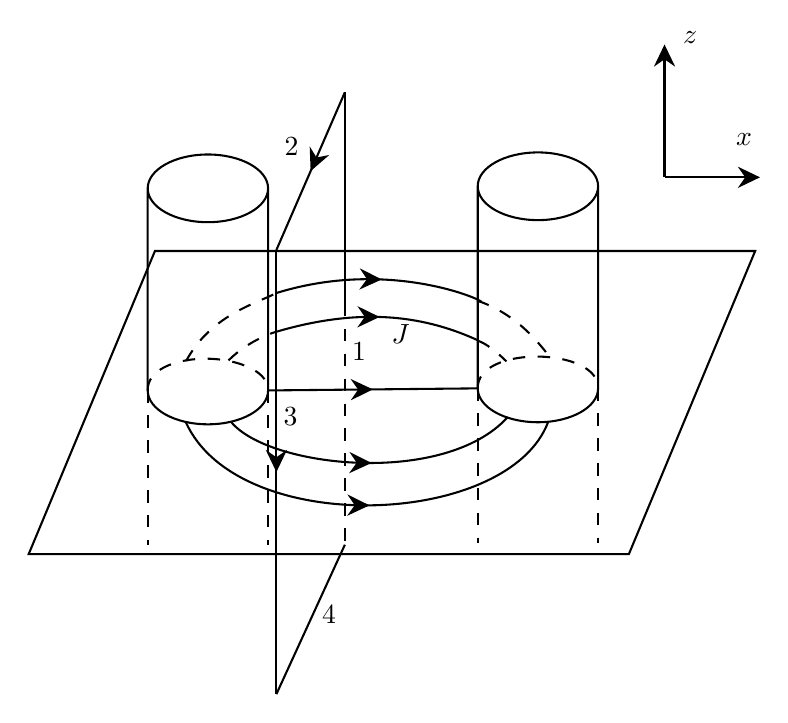
\begin{tikzpicture}[x=0.75pt,y=0.75pt,yscale=-1,xscale=1]
%uncomment if require: \path (0,450); %set diagram left start at 0, and has height of 450

%Shape: Parallelogram [id:dp590263130597569] 
\draw   (213.49,162.17) -- (502.67,162.17) -- (441.84,308.17) -- (152.67,308.17) -- cycle ;
%Straight Lines [id:da10295278078132264] 
\draw    (272,161.67) -- (272,375.67) ;
\draw [shift={(272,268.67)}, rotate = 270] [fill={rgb, 255:red, 0; green, 0; blue, 0 }  ][line width=0.08]  [draw opacity=0] (10.72,-5.15) -- (0,0) -- (10.72,5.15) -- (7.12,0) -- cycle    ;
%Straight Lines [id:da05143886065182923] 
\draw    (305,85.67) -- (272,161.67) ;
\draw [shift={(288.5,123.67)}, rotate = 293.47] [fill={rgb, 255:red, 0; green, 0; blue, 0 }  ][line width=0.08]  [draw opacity=0] (10.72,-5.15) -- (0,0) -- (10.72,5.15) -- (7.12,0) -- cycle    ;
%Straight Lines [id:da21347209362421404] 
\draw    (305,303.67) -- (272,375.67) ;
%Straight Lines [id:da26116284940289325] 
\draw    (305,85.67) -- (305,187.67) ;
%Straight Lines [id:da25015325740443073] 
\draw  [dash pattern={on 4.5pt off 4.5pt}]  (305,187.67) -- (305,303.67) ;
%Straight Lines [id:da35417729042825385] 
\draw    (459,65.67) -- (459,126.67) ;
\draw [shift={(459,62.67)}, rotate = 90] [fill={rgb, 255:red, 0; green, 0; blue, 0 }  ][line width=0.08]  [draw opacity=0] (10.72,-5.15) -- (0,0) -- (10.72,5.15) -- (7.12,0) -- cycle    ;
%Straight Lines [id:da7676077789544753] 
\draw    (459,126.67) -- (502,126.67) ;
\draw [shift={(505,126.67)}, rotate = 180] [fill={rgb, 255:red, 0; green, 0; blue, 0 }  ][line width=0.08]  [draw opacity=0] (10.72,-5.15) -- (0,0) -- (10.72,5.15) -- (7.12,0) -- cycle    ;
%Shape: Can [id:dp39072511191058923] 
\draw   (268,131.98) -- (268,229.35) .. controls (268,238.36) and (255.02,245.67) .. (239,245.67) .. controls (222.98,245.67) and (210,238.36) .. (210,229.35) -- (210,131.98) .. controls (210,122.97) and (222.98,115.67) .. (239,115.67) .. controls (255.02,115.67) and (268,122.97) .. (268,131.98) .. controls (268,140.99) and (255.02,148.29) .. (239,148.29) .. controls (222.98,148.29) and (210,140.99) .. (210,131.98) ;
%Shape: Can [id:dp4304850067909751] 
\draw   (427,130.98) -- (427,228.35) .. controls (427,237.36) and (414.02,244.67) .. (398,244.67) .. controls (381.98,244.67) and (369,237.36) .. (369,228.35) -- (369,130.98) .. controls (369,121.97) and (381.98,114.67) .. (398,114.67) .. controls (414.02,114.67) and (427,121.97) .. (427,130.98) .. controls (427,139.99) and (414.02,147.29) .. (398,147.29) .. controls (381.98,147.29) and (369,139.99) .. (369,130.98) ;
%Curve Lines [id:da4444465117732648] 
\draw  [dash pattern={on 4.5pt off 4.5pt}]  (210,229.35) .. controls (209.77,219.62) and (222.4,214.63) .. (235.94,214.07) .. controls (249.47,213.52) and (268.27,218.69) .. (268,229.35) ;
%Curve Lines [id:da5963569134271516] 
\draw  [dash pattern={on 4.5pt off 4.5pt}]  (369,228.35) .. controls (368.5,207.42) and (427.5,208.42) .. (427,228.35) ;
%Straight Lines [id:da8918846680127841] 
\draw  [dash pattern={on 4.5pt off 4.5pt}]  (210,229.35) -- (210,303.67) ;
%Straight Lines [id:da3353791073588641] 
\draw  [dash pattern={on 4.5pt off 4.5pt}]  (268,229.35) -- (268,303.67) ;
%Straight Lines [id:da31913748721329127] 
\draw  [dash pattern={on 4.5pt off 4.5pt}]  (369,228.35) -- (369,302.67) ;
%Straight Lines [id:da23772632524095938] 
\draw  [dash pattern={on 4.5pt off 4.5pt}]  (427,228.35) -- (427,263.67) -- (427,302.67) ;
%Curve Lines [id:da5377901186494225] 
\draw    (272,182.42) .. controls (331.5,163.92) and (380.2,190.17) .. (368.72,186.05) ;
\draw [shift={(322.75,175.88)}, rotate = 181.32] [fill={rgb, 255:red, 0; green, 0; blue, 0 }  ][line width=0.08]  [draw opacity=0] (10.72,-5.15) -- (0,0) -- (10.72,5.15) -- (7.12,0) -- cycle    ;
%Curve Lines [id:da8078946077416267] 
\draw  [dash pattern={on 4.5pt off 4.5pt}]  (368.72,186.05) .. controls (396,195.37) and (404.98,218.99) .. (404.98,212.49) ;
%Curve Lines [id:da4279646849736449] 
\draw    (228.27,244.43) .. controls (253.4,300.73) and (384.2,295.53) .. (403,244.33) ;
\draw [shift={(316.86,284.71)}, rotate = 180.62] [fill={rgb, 255:red, 0; green, 0; blue, 0 }  ][line width=0.08]  [draw opacity=0] (10.72,-5.15) -- (0,0) -- (10.72,5.15) -- (7.12,0) -- cycle    ;
%Curve Lines [id:da28756259240642534] 
\draw  [dash pattern={on 4.5pt off 4.5pt}]  (228.5,215.17) .. controls (240.5,192.92) and (262.5,187.42) .. (272,182.42) ;
%Curve Lines [id:da16134884964082885] 
\draw  [dash pattern={on 4.5pt off 4.5pt}]  (248.92,214.88) .. controls (259,204.78) and (271.89,201) .. (272.21,201) ;
%Curve Lines [id:da21745721003301255] 
\draw    (272.21,201) .. controls (314.67,188.54) and (344.92,194.04) .. (369.47,205.37) ;
\draw [shift={(321.72,193.95)}, rotate = 180.38] [fill={rgb, 255:red, 0; green, 0; blue, 0 }  ][line width=0.08]  [draw opacity=0] (10.72,-5.15) -- (0,0) -- (10.72,5.15) -- (7.12,0) -- cycle    ;
%Curve Lines [id:da3580325468052228] 
\draw  [dash pattern={on 4.5pt off 4.5pt}]  (369.47,205.37) .. controls (368.17,205.53) and (372.67,205.31) .. (382.83,215.36) ;
%Curve Lines [id:da5604816867368483] 
\draw    (250.03,244.33) .. controls (267.85,266.58) and (353.12,275.85) .. (383.48,242.15) ;
\draw [shift={(317.81,264.3)}, rotate = 180.96] [fill={rgb, 255:red, 0; green, 0; blue, 0 }  ][line width=0.08]  [draw opacity=0] (10.72,-5.15) -- (0,0) -- (10.72,5.15) -- (7.12,0) -- cycle    ;
%Straight Lines [id:da42647618453854275] 
\draw    (268,229.35) -- (369,228.35) ;
\draw [shift={(318.5,228.85)}, rotate = 539.4300000000001] [fill={rgb, 255:red, 0; green, 0; blue, 0 }  ][line width=0.08]  [draw opacity=0] (10.72,-5.15) -- (0,0) -- (10.72,5.15) -- (7.12,0) -- cycle    ;

% Text Node
\draw (466.5,55.07) node [anchor=north west][inner sep=0.75pt]    {$z$};
% Text Node
\draw (492,104.07) node [anchor=north west][inner sep=0.75pt]    {$x$};
% Text Node
\draw (274.5,106.07) node [anchor=north west][inner sep=0.75pt]    {$2$};
% Text Node
\draw (274,236.07) node [anchor=north west][inner sep=0.75pt]    {$3$};
% Text Node
\draw (307,205.07) node [anchor=north west][inner sep=0.75pt]    {$1$};
% Text Node
\draw (292.5,331.57) node [anchor=north west][inner sep=0.75pt]    {$4$};
% Text Node
\draw (326,196.07) node [anchor=north west][inner sep=0.75pt]    {$J$};


\end{tikzpicture}

    \end{center}
    \begin{center}
        \textbf{Hình 4.} Mạch Ampere
    \end{center}
   Với đường dẫn này, ta cần tính dòng điện chạy qua mạch
    \[I=\int\overrightarrow{J}\mathrm{d}\overrightarrow{A}=\int Jx\ell\mathrm{d}y=\dfrac{V_0\delta\ell}{2\ln{3}}\left(\dfrac{4a+x}{(4a+x)^2+y^2}+\dfrac{4a-x}{(4a-x)^2+y^2}\right)\mathrm{d}y.\]
    \[I=\dfrac{V_0\sigma\ell}{\ln{3}}\left(\arctan{\dfrac{y}{4a+x}}+\arctan{\dfrac{y}{4a-x}}\right). \tag{29} \label{apho13sa.29}\]
    Khi dùng định luật Ampere,
    \[\oint\ot{B}\mathrm{d}\ot{I}=\mu_0I. \tag{30} \label{apho13sa.30}\]
    
    \begin{align*}
        \Rightarrow2B_{z}\ell &= \dfrac{\mu_0V_0\sigma\ell}{\ln{3}}\left(\arctan{\dfrac{y}{4a+x}+\arctan{\dfrac{y}{4a-x}}}\right),\\
        \Rightarrow B_{z} &= \dfrac{\mu_0V_0\sigma}{2\ln{3}}\left(\arctan{\dfrac{y}{4a+x}+\arctan{\dfrac{y}{4a-x}}}\right), \tag{31} \label{apho13sa.31}\\
        \Rightarrow\ot{B} &= \ot{z}\dfrac{\mu_0V_0\sigma}{2\ln{3}}\left(\arctan{\dfrac{y}{4a+x}+\arctan{\dfrac{y}{4a-x}}}\right). \tag{32} \label{apho13sa.32}
    \end{align*}
    
\end{enumerate}
\end{loigiai}

\begin{vd}[Gia tốc cho sóng xung kích]
Trong không gian vũ trụ, sóng xung kích có thể gia tốc cho các hạt mang điện cho đến khi đạt được một mức năng lượng rất cao. Chúng ta có thể sử dụng một mô hình lí tưởng của sóng xung kích và thừa nhận rằng có tồn tại một màn chắn thế năng là $-V_0$ được đặt ở chiều cao không đổi và chuyển động với vận tốc $\omega$ quanh trục $Ox$:
\[\begin{aligned}
    &V(x,y,z,t)=-V_0 &\text{nếu } x<\omega t;\\
    &V(x,y,z,t)=0 &\text{nếu } x>\omega t.
\end{aligned}\]
Trong hệ quy chiếu không có sóng xung kích, năng lượng của electron được bảo toàn. Điều đó có nghĩa rằng miễn là khi động năng của electron có khối lượng $m$ và có điện tích $-e$ nhỏ hơn năng lượng của sóng xung kích ($\dfrac{1}{2}mu^2<eV_0 $, với $u$ là vận tốc của electron chuyển động trong môi trường có sóng xung kích), nó sẽ bị phản xạ lại giống như cách một quả bóng đàn hồi bật lại khi va chạm với một bức tường cứng. Sau đây, trừ khi được đề cập trong những trường hợp đặc biệt, va chạm của electron với sóng xung kích sẽ là va chạm đàn hồi. Bạn có thể sẽ phải dùng các thông số như $e$, $V_0$, $m$, $B$, và $\omega$ để biểu diễn các kết quả. Trừ khi ở trong những trường hợp đặc biệt, vận tốc của electron được xem là phi tương đối tính.
\begin{enumerate}[1)]
    \item Cho vận tốc đầu của electron là $\overrightarrow{v}=(v_{x}, v_{y}, v_{z})$ với $v_{x}<\omega$. Hãy xác định vận tốc $\overrightarrow{v'}$ (nói cách khác là các thành phần $v'_{x}, v'_{y}, v'_{z}$) của electron ngay sau khi va chạm với sóng xung kích.
    \item Bây giờ, ở đó cũng có một từ trường đều có cảm ứng từ là $B$, song song với trục $Oz$. Tại thời điểm bắt đầu, electron đang đứng yên ở gốc tọa độ, tại thời điển $t=0$ thì chịu tác dụng của sóng xung kích. Hãy vẽ phác thảo quỹ đạo định tính của electron từ lúc bắt đầu $t=0$ đến ít nhất là lúc $t=\dfrac{\pi m}{Be}$.
    \item Tìm bán kính cong của quỹ đạo electron ngay sau lần va chạm đầu tiên với sóng xung kích.
    \item Tại thời điểm $t_2$, electron sẽ xảy ra va chạm lần thứ hai. Hãy viết biểu thức để xác định $t_2$. Hãy áp dụng phép tính bằng số để biểu diễn $t_2$.
    \item Hãy xác định vận tốc trung bình theo phương $Ox$ $(v_{x})$ của electron (trung bình trong khoảng thười gian $\tau$ giữa hai lần va chạm liên tiếp của electron với sóng xung kích).
    \item Theo thời gian, electron sẽ va chạm rất nhiều lần với sóng xung kích. Hãy chứng minh rằng trong suốt quá trình chuyển động, $v_{y}+kx=$ hằng số, với $k$ là hằng số; biểu diễn $k$ theo $e$, $m$ và $B$.$\label{6}$
    \item Từ bây giờ, chúng ta sẽ xem xét giới hạn $t\gg \dfrac{2\pi m}{Be}$. Xác định gia tốc trung bình theo phương $Oy$ của electron (biểu diễn theo $e$, $m$ và $B$ hay hằng số $k$ đã được giới thiệu ở phần \ref{6}).
    \item Có một vấn đề xuất hiện đó là tại giới hạn $t \gg \dfrac{2\pi m}{Be}$, khoảng thời gian $\tau$ giữa hai lần va chạm ngày càng ngắn dần, vì thế chúng ta có thể thừa nhận rằng $\tau \ll \dfrac{2\pi m}{Be}$. Điều đó có nghĩa là trong khoảng thòi gian giữa hai lần va chạm, vector vận tốc của electron sẽ chỉ đổi một góc rất nhỏ và do đó, vector gia tốc $\overrightarrow{a}=(a_{x},a_{y})$ có thể xem như là bảo toàn.\\
    Bây giờ chúng ta sẽ sử dụng hệ quy chiếu gắn với sóng xung kích, chúng ta xem xét đồ thị pha của electron, nói cách khác là đồ thị mô tả trạng thái của electron như một điểm trong mặt phẳng $x'$ $-$ $p'_{x}$ với trục tung là $p'_{x}=m(v_{x}-\omega)$ tương ứng với $x'$ $-$ thành phần của động lượng, và $x'=\di\int(v_{x}-\omega) \mathrm{d}t$ là khoảng cách so với sóng xung kích. Hãy mô tả một cách định tính quỹ đạo pha của electron, nói cách khác là các đường cong trong đồ thị pha trong suốt một giai đoạn (giữa hai lần va chạm liên tiếp của electron và sóng xung kích). Điểm của phần này sẽ dựa hoàn toàn vào hình dạng của đường cong.
    \item Theo thời gian, độ rộng và chiều cao của quỹ đạo pha sẽ thay đổi, tuy nhiên, có một điều là diện tích bề mặt của vùng được bao bởi quỹ đạo pha (được gọi là bất biến đoạn nhiệt) sẽ luôn là hằng số với độ chính xác cao. Đối với một electron ban đầu ở trạng thái nghỉ, bất biến đoạn nhiệt có giá trị xấp xỉ bằng $\dfrac{1,36(m\omega)^2}{Be}$. Hãy xác định tổng động năng $W_{f}$ của electron khi nó bị tụt lại đằng sau so với sóng xung kích; biểu diễn theo $e$, $V_0$ và $\varepsilon$ với định nghĩa rằng $\varepsilon=\dfrac{2eV_0}{m\omega^2}$;  biết rằng $\varepsilon \gg 1$.
    \item Câu hỏi cuối cùng này sẽ độc lập so với những câu hỏi trước. Xem xét sự lan truyền của sóng xung kích như đã mô tả ở phần trước, nhưng không có sự xuất hiện của từ trường. Một electron tương đối sẽ chuyển động song song so với mặt trước (trong hệ quy chiếu phòng thí nghiệm, thành phần tiếp tuyến của vận tốc luôn bằng không). Biết rằng $m\omega^2<eV_0$ và $\omega \ll c$ (với $c$ là vận tốc ánh sáng), năng lượng tương đối của electron để có thể bị tụt lại phía sau so với sóng xung kích là bao nhiêu? Bạn có thể sử dụng bất kì sự làm tròn hay lấy xấp xỉ nào, miễn là nó hợp lí.
\end{enumerate}
\end{vd}
\begin{loigiai}
\begin{enumerate}[1)]
    \item Trong hệ quy chiếu gắn với sóng xung kích, vận tốc ban đầu của electron là $$\overrightarrow{v_1}=(v_{x}-\omega,v_{y}, v_{z}).$$ 
    Sau khi bị lệch khỏi sóng xung kích, thành phần nằm ngang của vận tốc bị đảo chiều. Do đó, vận tốc của electron trong hệ quy chiếu phi quán tính đang chuyển động, sau khi bị đảo chiều sẽ là $\overrightarrow{v_2}=(\omega-v_{x}, v_{y}, v_{z})$. Quay trở lại với hệ quy chiếu phòng thí nghiệm, cuối cùng vận tốc của electron là $\overrightarrow{v'}=(2\omega-v_{x}, v_{y}, v_{z})$.
    \item Sau khi va chạm với sóng xung kích, electron bắt đầu chuyển động với tốc độ $v=2\omega$. Do từ trường, electron sẽ chuyển động theo quỹ đạo tròn, và tại thời điểm ban đầu, quỹ đạo đó vuông góc với mặt trước. Thêm vào đó, electron sẽ va chạm với sóng xung kích theo chu kì, và tọa độ $x$ của các lần va chạm đó sẽ tăng dần theo thời gian. Điều đó đủ để chúng ta phác họa tương đối quỹ đạo của electron.
\begin{center}
\tikzset{every picture/.style={line width=0.75pt}} %set default line width to 0.75pt        

\begin{tikzpicture}[x=0.75pt,y=0.75pt,yscale=-1,xscale=1]
%uncomment if require: \path (0,300); %set diagram left start at 0, and has height of 300

%Straight Lines [id:da5591323659404421] 
\draw    (220,233.33) -- (220,43.33) ;
\draw [shift={(220,40.33)}, rotate = 450] [fill={rgb, 255:red, 0; green, 0; blue, 0 }  ][line width=0.08]  [draw opacity=0] (10.72,-5.15) -- (0,0) -- (10.72,5.15) -- (7.12,0) -- cycle    ;
%Straight Lines [id:da7603110770757822] 
\draw    (170,80.33) -- (409,80.33) ;
\draw [shift={(412,80.33)}, rotate = 180] [fill={rgb, 255:red, 0; green, 0; blue, 0 }  ][line width=0.08]  [draw opacity=0] (10.72,-5.15) -- (0,0) -- (10.72,5.15) -- (7.12,0) -- cycle    ;
%Curve Lines [id:da7222425082975721] 
\draw    (220,80.33) .. controls (237,82.33) and (259,90.33) .. (259,123) ;
%Curve Lines [id:da3306653270482587] 
\draw    (259,123) .. controls (277,124.33) and (300,143.33) .. (298,165.67) ;
%Curve Lines [id:da3075618074644175] 
\draw    (298,165.67) .. controls (319.12,173.99) and (330.1,199.2) .. (330.06,221.56) ;
\draw [shift={(330,224.33)}, rotate = 272.49] [fill={rgb, 255:red, 0; green, 0; blue, 0 }  ][line width=0.08]  [draw opacity=0] (10.72,-5.15) -- (0,0) -- (10.72,5.15) -- (7.12,0) -- cycle    ;

% Text Node
\draw (389,86.4) node [anchor=north west][inner sep=0.75pt]    {$x$};
% Text Node
\draw (200,46.4) node [anchor=north west][inner sep=0.75pt]    {$y$};


\end{tikzpicture}
\end{center}
    \item Lực Lorentz tác dụng lên electron đóng vai trò là lực hướng tâm:
    \[evB_0=\dfrac{mv^2}{R}.\]
 Do đó: \[R=\dfrac{mv}{eB_0}=\dfrac{2m\omega}{eB_0}.\]

    \item Trước lần va chạm đầu tiên, tọa độ $x$ của electron là $x_1(t)=R\sin{\left(2\pi\dfrac{t}{T}\right)}$ và tọa độ $x$ của sóng xung kích là $x_2(t)=\omega t$. Lần va chạm thứ hai xảy ra khi $x_1(t)=x_2(t)$. Do đó:
    \begin{align*}
    \dfrac{2m\omega}{eB_0}\sin{\left(\dfrac{B_0e}{m}t_2\right)}&=\omega t_2,\\
    \sin{\left(\dfrac{B_0e}{m}t_2\right)}&=\dfrac{1}{2}\dfrac{B_0e}{m}t_2.
    \end{align*}
    Thay $u=\dfrac{B_0e}{m}t_2$, ta được:
    \[\sin{u}=\dfrac{u}{2}.\]
    Đẳng thức này cho nghiệm là $u=1,895$. Do đó: $t_2=1,895 \dfrac{m}{B_0e}$.
    \item Mỗi khi xảy ra va chạm, electron và mặt phẳng phía trước luôn ở cùng vị trí, với cùng giá trị tọa độ $x$. Điều đó có nghĩa là vận tốc trung bình của electron và của sóng xung kích theo phương trục $Ox$ luôn giống nhau. Hay nói cách khác $v_{x}=\omega$.
    \item Chúng ta dễ dàng tìm được giá trị của $k$ bằng cách đạo hàm hai vế của đẳng thức vì các hằng số đã bị loại bỏ. Do đó $\Dot{v_{y}}+kv_{x}=0$. Những lực duy nhất tác dụng lên electron chính là lực Lorentz và lực đẩy giữa electron và sóng xung kích. Vì sóng xung kích tác dụng lên electron chỉ theo phương nằm ngang, thành phần gia tốc theo phương thẳng đứng được tạo ra hoàn toàn dựa vào lực Lorentz. Điều đó có nghĩa là $m\Ddot{y}=-ev_{x}B_0$ được giữ xuyên suốt trong qua trình chuyển động của electron. Nói cách khác, $\Dot{v_{y}}=-\dfrac{B_0e}{m}v_{x}$. Kết hợp với định luật bảo toàn năng lượng, chúng ta có $-\dfrac{B_0e}{m}v_{x}+kv_{x}=0$. Do đó $k=\dfrac{B_0e}{m}$.
    \item Bằng cách đạo hàm từ định luật bảo toàn $v_{y}+\dfrac{B_0e}{m}x=$ hằng số, chúng ta có $a_{y}+\dfrac{B_0e}{m}v_{x}=0$. Trong một thời gian dài, tốc độ chuyển động trung bình của electron theo trục $Ox$ sẽ giống như tốc độ của sóng xung kích. Do đó $a_{y}+\dfrac{B_0e}{m}\omega=0$ và $a_{y}=-\dfrac{B_0e}{m}\omega$.
    \item Trong một khoảng thời gian, luôn có một gia tốc không đổi $a_{x}$ tác dụng lên electron theo phương $Ox$, kể cả trong hệ quy chiếu phòng thí nghiệm và hệ quy chiếu sóng xung kích; chuyển động sẽ giống như bình thường nếu có gia tốc rơi tự do $g=a$. Nếu chúng ta gọi $x$ là khoảng cách tương đối giữa electron và sóng xung kích, động lượng ban đầu theo phương $Ox$ tại $x=0$ là $p_{x0}$, và năng lượng $E=\dfrac{p_{x0}^2}{2m}=\dfrac{p^2_{x}}{2m}+ma_{x}x$ được bảo toàn trong suốt khoảng thời gian ấy (định luật bảo toàn năng lượng). Do đó $p_{x}=\sqrt{p^2_{x0}-2m^2a_{x}x}$. Trên đồ thị pha, nó biểu diễn bằng một đường parabol với trục đối xứng tại $p_{x}=0$. Hơn thế nữa, tại $x=0$, động lượng của electron bị đảo chiều do sự va chạm với sóng xung kích, điều đó có nghĩa là sẽ có một đường thẳng từ $(0,-p_{x0})$ đến $(0,p_{x0})$. Từ những dữ kiện trên, ta có thể vẽ đồ thị pha như sau:
    \begin{center}
% Pattern Info
 
\tikzset{
pattern size/.store in=\mcSize, 
pattern size = 5pt,
pattern thickness/.store in=\mcThickness, 
pattern thickness = 0.3pt,
pattern radius/.store in=\mcRadius, 
pattern radius = 1pt}
\makeatletter
\pgfutil@ifundefined{pgf@pattern@name@_obp51fhcq}{
\pgfdeclarepatternformonly[\mcThickness,\mcSize]{_obp51fhcq}
{\pgfqpoint{0pt}{0pt}}
{\pgfpoint{\mcSize+\mcThickness}{\mcSize+\mcThickness}}
{\pgfpoint{\mcSize}{\mcSize}}
{
\pgfsetcolor{\tikz@pattern@color}
\pgfsetlinewidth{\mcThickness}
\pgfpathmoveto{\pgfqpoint{0pt}{0pt}}
\pgfpathlineto{\pgfpoint{\mcSize+\mcThickness}{\mcSize+\mcThickness}}
\pgfusepath{stroke}
}}
\makeatother
\tikzset{every picture/.style={line width=0.75pt}} %set default line width to 0.75pt        

\begin{tikzpicture}[x=0.75pt,y=0.75pt,yscale=-1,xscale=1]
%uncomment if require: \path (0,300); %set diagram left start at 0, and has height of 300

%Straight Lines [id:da5313724387613878] 
\draw    (162,180.33) -- (391,180.33) ;
\draw [shift={(394,180.33)}, rotate = 180] [fill={rgb, 255:red, 0; green, 0; blue, 0 }  ][line width=0.08]  [draw opacity=0] (10.72,-5.15) -- (0,0) -- (10.72,5.15) -- (7.12,0) -- cycle    ;
%Straight Lines [id:da5968701993643626] 
\draw    (240,260.33) -- (240,75.33) ;
\draw [shift={(240,72.33)}, rotate = 450] [fill={rgb, 255:red, 0; green, 0; blue, 0 }  ][line width=0.08]  [draw opacity=0] (10.72,-5.15) -- (0,0) -- (10.72,5.15) -- (7.12,0) -- cycle    ;
%Shape: Parabola [id:dp40594583338022083] 
\draw  [pattern=_obp51fhcq,pattern size=6pt,pattern thickness=0.75pt,pattern radius=0pt, pattern color={rgb, 255:red, 0; green, 0; blue, 0}] (240.24,220.92) .. controls (331.53,191.15) and (331.61,161.14) .. (240.47,130.9) ;
%Straight Lines [id:da5900835283967321] 
\draw    (255,215.67) -- (243.06,219.92) ;
\draw [shift={(240.24,220.92)}, rotate = 340.4] [fill={rgb, 255:red, 0; green, 0; blue, 0 }  ][line width=0.08]  [draw opacity=0] (10.72,-5.15) -- (0,0) -- (10.72,5.15) -- (7.12,0) -- cycle    ;
%Straight Lines [id:da4587777282898413] 
\draw    (240,146) -- (240.38,133.9) ;
\draw [shift={(240.47,130.9)}, rotate = 451.79] [fill={rgb, 255:red, 0; green, 0; blue, 0 }  ][line width=0.08]  [draw opacity=0] (10.72,-5.15) -- (0,0) -- (10.72,5.15) -- (7.12,0) -- cycle    ;
%Straight Lines [id:da6091201871513336] 
\draw    (309,172) -- (308.87,176.09) ;
\draw [shift={(308.77,179.09)}, rotate = 271.86] [fill={rgb, 255:red, 0; green, 0; blue, 0 }  ][line width=0.08]  [draw opacity=0] (10.72,-5.15) -- (0,0) -- (10.72,5.15) -- (7.12,0) -- cycle    ;

% Text Node
\draw (218,77.4) node [anchor=north west][inner sep=0.75pt]    {$p_{x}$};
% Text Node
\draw (377,185.4) node [anchor=north west][inner sep=0.75pt]    {$x$};
% Text Node
\draw (310,185.4) node [anchor=north west][inner sep=0.75pt]    {$x_{1}$};
% Text Node
\draw (210,117.4) node [anchor=north west][inner sep=0.75pt]    {$p_{x0}$};
% Text Node
\draw (204,212.4) node [anchor=north west][inner sep=0.75pt]    {$-p_{x0}$};


\end{tikzpicture}

    \end{center}
    \item Diện tích phần dưới của biểu đồ pha có thể tìm bằng cách lấy tích phân $p_{x}(x)\mathrm{d}x$ từ $x_0=0$ đến $x_1=\dfrac{p^2_{x0}}{2m^2a_{x}}$ và nhân đôi kết quả với $2$ (bởi vì đồ thị pha đối xứng qua $p_{x}=0$). Do đó:
    \[S=2\int_{0}^{x_1}\sqrt{p^2_{x0}-2m^2a_{x}x}~\mathrm{d}x=2p_{x0}\int_{0}^{x_1}\sqrt{1-\dfrac{x}{x_1}}~\mathrm{d}x=\dfrac{4}{3}p_{x0}x_1=\dfrac{2}{3}\dfrac{p^3_{x0}}{m^2a_{x}}=\dfrac{2}{3}\dfrac{mv_0^3}{a_{x}}.\]
    Do sự bảo toàn của đại lượng này (chúng ta sử dụng giá trị ban đầu của nó từ dữ kiện đề bài)
    \begin{align*}
    \dfrac{2}{3}\dfrac{mv_0^3}{a_{x}}&=\dfrac{1,36(m\omega)^2}{B_0e},\\
    a_{x}&=\dfrac{1}{2,04}\dfrac{v_0^3B_0e}{m\omega^2}.
    \end{align*}
    Với $v_0$ là tốc độ của electron tại $x=0$. Electron sẽ bị tụt lại phía sau so với sóng xung kích khi $\dfrac{mv_0^2}{2}>eV_0$ hay $v_0>\sqrt{\dfrac{2eV_0}{m}}=\omega\sqrt{\varepsilon}$. Thành phần gia tốc nằm ngang là do lực Lorentz $a_{x}=\dfrac{B_0ev_{y}}{m}$. Do đó:
    %d - displaystyle
    \begin{align*}
        \dfrac{1}{2,04}\dfrac{B_0e}{m\omega^2}\omega^3\varepsilon^{ \frac{3}{2}}&=\dfrac{B_0ev_{y}}{m},\\
        \dfrac{1}{2,04}\omega\varepsilon^{ \frac{3}{2}}&=v_{y}.
    \end{align*}
    Vì $v_{y} \gg v_{x}$, $W_{f}\approx\dfrac{mv^2_{y}}{2}$
    \[W_{f}=\dfrac{\varepsilon^3}{2,04}\dfrac{m\omega^2}{2}=\dfrac{\varepsilon^2}{2,04^2}eV_0.\]
    \item Trong hệ quy chiếu gắn với sóng xung kích, ban đầu, động lượng tác dụng theo phương $Ox$ và $Oy$ lần lượt là $p_{x}$ và $p_{y}$. Trong trường hợp giới hạn, động lượng cuối cùng của electron theo phương $Ox$ là bằng không. Do sóng xung kích chỉ có tác dụng theo phương $Ox$, $p_{y}$ vẫn giữ nguyên không đổi trong suốt quá trình chuyển động. Đại lượng bất biến Lorentz động lượng bốn chiều trước và sau khi electron đạt được trạng thái nghỉ, có thể viết như sau:
    \begin{align*}
        E^2&=p_{x}^2c^2+p_{y}^2c^2+m_0^2c^4,\\
        (E-eV_0)^2&=p_{y}^2c^2+m_0^2c^4.
    \end{align*}
Trừ vế theo vế, ta được $2EeV_0-e^2V_0^2=p_{x}^2c^2=m^2_{\text{rel}}c^2\omega^2=E^2\dfrac{\omega^2}{c^2}$. Do đó:
\[\begin{aligned}
    &E^2\dfrac{\omega^2}{c^2}-2EeV_0+e^2V_0^2 = 0,\\
    &E = \dfrac{eV_0c^2}{\omega^2}\left(1\pm\sqrt{1-\dfrac{\omega^2}{c^2}}\right),
\end{aligned}\]
với dấu trừ chúng ta có thể thu được $p_{y}^2c^2=(E-eV_0)^2-m_0^2c^4<(E-eV_0)^2-e^2V_0^2c^4/\omega^4<0$ là điều không đúng. Do đó, chúng ta phải lấy dấu cộng:
\[E=\dfrac{eV_0c^2}{\omega^2}\left(1+\sqrt{1-\dfrac{\omega^2}{c^2}}\right),\]
trong đó, $\omega \ll c$ nên chúng ta có thể lấy gần đúng $E=\dfrac{2eV_0c^2}{\omega^2}$. Vậy electron sẽ bị tụt lại phía sau so với sóng xung kích nếu năng lượng tương đối của nó là $E\geq\dfrac{2eV_0c^2}{\omega^2}$.
\end{enumerate}
\end{loigiai}


\begin{vd}[Electron thoát ra]
    Một dây dẫn dài vô hạn có dòng điện $I$ và bán kính $a$.
    \begin{enumerate}[1)]
    %\setlength{\itemsep}{-5pt}
        \item Bề mặt bên ngoài của dây được giữ ở điện thế $-V$, với $V$ dương. Dây dẫn được đặt trong một lớp vỏ hình trụ được nối đất với bán kính $b>a$. Bằng một cách nào đó, một electron thoát ra khỏi bề mặt dây dẫn. Coi rằng lúc thoát ra khỏi bề mặt dây dẫn, electron có vận tốc bằng không. Bỏ qua sự bức xạ điện từ.\\
        Vẽ một cách định tính đường đi của elctron cùng với dây.
        \item Tìm khoảng cách cực đại $r_{\max}$ của electron đến trục dây trong quá trình chuyển động của electron theo $V$, $I$, $a$ và $b$.
        Bỏ qua hiệu ứng tương đối tính.
        \item Câu hỏi như phần trên nhưng có tính đến hiệu ứng tương đối tính.
        \item Vẽ đồ thị $r_{\max}$ theo như tính được trong phần $3)$ như là một hàm của $V$.
    \end{enumerate}
    \end{vd}
      \begin{loigiai}
      \renewcommand{\theequation}{\arabic{equation}}
    \begin{enumerate}[1)]
    \setlength{\itemsep}{0pt}
        \item Ta thấy các lực tác dụng chỉ nằm trong mặt phẳng đi qua trục dây dẫn, vậy nên electron chỉ chuyển động trong mặt phẳng đi qua trục dây dẫn.\\
        Hình dạng quỹ đạo của electron như hình vẽ.
        %chèn hình
        \begin{center}
            

\tikzset{every picture/.style={line width=0.75pt}} %set default line width to 0.75pt        

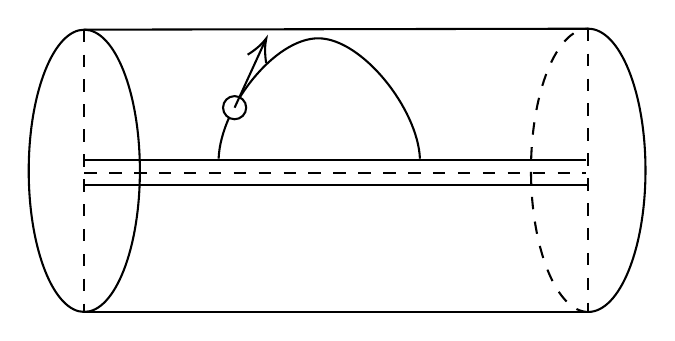
\begin{tikzpicture}[x=0.75pt,y=0.75pt,yscale=-1,xscale=1]
%uncomment if require: \path (0,210); %set diagram left start at 0, and has height of 210

%Straight Lines [id:da5620675167927436] 
\draw    (187,106) -- (428.71,106) ;
%Straight Lines [id:da13390227703886715] 
\draw    (187,118) -- (429.71,118) ;
%Straight Lines [id:da2539571226839463] 
\draw  [dash pattern={on 4.5pt off 4.5pt}]  (187,112) -- (428.71,112) ;
%Straight Lines [id:da9224449183978367] 
\draw    (187,43) -- (429.68,42.54) ;
%Straight Lines [id:da6358504813067694] 
\draw    (187,179) -- (429.71,179) ;
%Curve Lines [id:da9477997558507147] 
\draw    (251.71,105.16) .. controls (252.71,80.16) and (278.71,47.16) .. (299.71,47.16) .. controls (320.71,47.16) and (347.71,81.16) .. (348.71,105.16) ;
%Shape: Circle [id:dp31182285601982773] 
\draw  [fill={rgb, 255:red, 255; green, 255; blue, 255 }  ,fill opacity=1 ] (253.84,80.58) .. controls (253.84,77.5) and (256.34,75) .. (259.42,75) .. controls (262.5,75) and (265,77.5) .. (265,80.58) .. controls (265,83.66) and (262.5,86.16) .. (259.42,86.16) .. controls (256.34,86.16) and (253.84,83.66) .. (253.84,80.58) -- cycle ;
%Straight Lines [id:da13951558247655105] 
\draw    (259.42,80.58) -- (273.88,48.97) ;
\draw [shift={(274.71,47.16)}, rotate = 474.58] [color={rgb, 255:red, 0; green, 0; blue, 0 }  ][line width=0.75]    (10.93,-4.9) .. controls (6.95,-2.3) and (3.31,-0.67) .. (0,0) .. controls (3.31,0.67) and (6.95,2.3) .. (10.93,4.9)   ;
%Shape: Ellipse [id:dp32197955614831475] 
\draw   (160.22,111) .. controls (160.22,73.44) and (172.21,43) .. (187,43) .. controls (201.79,43) and (213.78,73.44) .. (213.78,111) .. controls (213.78,148.56) and (201.79,179) .. (187,179) .. controls (172.21,179) and (160.22,148.56) .. (160.22,111) -- cycle ;
%Shape: Arc [id:dp8110209425106236] 
\draw  [draw opacity=0] (429.68,42.54) .. controls (429.72,42.54) and (429.76,42.54) .. (429.79,42.54) .. controls (445.03,42.54) and (457.38,73.09) .. (457.38,110.77) .. controls (457.38,148.45) and (445.03,179) .. (429.79,179) .. controls (429.76,179) and (429.74,179) .. (429.71,179) -- (429.79,110.77) -- cycle ; \draw   (429.68,42.54) .. controls (429.72,42.54) and (429.76,42.54) .. (429.79,42.54) .. controls (445.03,42.54) and (457.38,73.09) .. (457.38,110.77) .. controls (457.38,148.45) and (445.03,179) .. (429.79,179) .. controls (429.76,179) and (429.74,179) .. (429.71,179) ;
%Shape: Arc [id:dp8017528716240261] 
\draw  [draw opacity=0][dash pattern={on 4.5pt off 4.5pt}] (429.9,179) .. controls (429.86,179) and (429.83,179) .. (429.79,179) .. controls (414.56,179) and (402.21,148.45) .. (402.21,110.77) .. controls (402.21,73.09) and (414.56,42.54) .. (429.79,42.54) .. controls (429.82,42.54) and (429.85,42.54) .. (429.87,42.54) -- (429.79,110.77) -- cycle ; \draw  [dash pattern={on 4.5pt off 4.5pt}] (429.9,179) .. controls (429.86,179) and (429.83,179) .. (429.79,179) .. controls (414.56,179) and (402.21,148.45) .. (402.21,110.77) .. controls (402.21,73.09) and (414.56,42.54) .. (429.79,42.54) .. controls (429.82,42.54) and (429.85,42.54) .. (429.87,42.54) ;
%Straight Lines [id:da2798876105658161] 
\draw  [dash pattern={on 4.5pt off 4.5pt}]  (187,43) -- (187,179) ;
%Straight Lines [id:da9391813698918585] 
\draw  [dash pattern={on 4.5pt off 4.5pt}]  (429.87,42.54) -- (429.87,178.54) ;




\end{tikzpicture}

        \end{center}
        \item Giả sử điện trường tại bề mặt dây dẫn là $E_0$.\\
        Áp dụng định luật Gauss, ta có:
        \begin{equation*}
        \begin{aligned}
             E_0\tron{2\pi al}&=E(r)\tron{2\pi rl},\\
             \Leftrightarrow E(r)&=\dfrac{E_0a}{r}.
        \end{aligned}
        \end{equation*}
        Lại có:
        \[\begin{aligned}
            \dd V&=-E(r)\dd r,\\
            \Leftrightarrow  \dd V&=-E_0a\frac{\dd r}{r},\\
            \Leftrightarrow \ V_r&=E_0a\ln\tron{\dfrac{b}{r}}.
        \end{aligned}\tag{1}\label{c161}\]
        Tại $r=a$ thì $V_r=-V$, suy ra:
        $$ -V=E_0a\ln\tron{\dfrac{b}{a}}\Leftrightarrow E_0=\dfrac{-V}{a\ln\tron{\dfrac{b}{a}}}.$$
        Thay vào (\ref{c161}), ta có:
        $$V_r=-V\dfrac{\ln\dfrac{b}{r}}{\ln\dfrac{b}{a}}=V\log_{\frac{b}{a}}\tron{\dfrac{r}{b}}.$$
        Từ trường sinh ra bởi dây dẫn:
        $$B(r)=\dfrac{\mu_0I}{2\pi r}.$$
        Gọi $v_r$, $v_z$ lần lượt là thành phần vận tốc theo phương bán kính và theo phương song song với trục dây.\\
        \begin{minipage}{0.5\textwidth}
             
\centering
\tikzset{every picture/.style={line width=0.75pt}} %set default line width to 0.75pt        

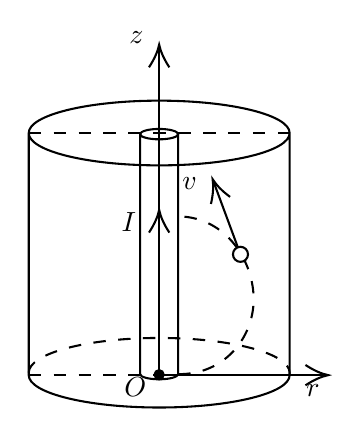
\begin{tikzpicture}[x=0.75pt,y=0.75pt,yscale=-1,xscale=1]
%uncomment if require: \path (0,210); %set diagram left start at 0, and has height of 210

%Straight Lines [id:da3973766845775675] 
\draw    (389.02,122.2) -- (376.29,87.85) ;
\draw [shift={(375.6,85.98)}, rotate = 429.65999999999997] [color={rgb, 255:red, 0; green, 0; blue, 0 }  ][line width=0.75]    (10.93,-4.9) .. controls (6.95,-2.3) and (3.31,-0.67) .. (0,0) .. controls (3.31,0.67) and (6.95,2.3) .. (10.93,4.9)   ;
%Shape: Can [id:dp15135767507223008] 
\draw   (412.71,63.75) -- (412.71,180.41) .. controls (412.71,189.02) and (384.57,196) .. (349.85,196) .. controls (315.14,196) and (287,189.02) .. (287,180.41) -- (287,63.75) .. controls (287,55.14) and (315.14,48.16) .. (349.85,48.16) .. controls (384.57,48.16) and (412.71,55.14) .. (412.71,63.75) .. controls (412.71,72.36) and (384.57,79.34) .. (349.85,79.34) .. controls (315.14,79.34) and (287,72.36) .. (287,63.75) ;
%Straight Lines [id:da7332224525248945] 
\draw  [dash pattern={on 4.5pt off 4.5pt}]  (287,180.41) -- (412.71,180.41) ;
%Straight Lines [id:da25208598259641724] 
\draw    (349.85,23.16) -- (349.85,180.41) ;
\draw [shift={(349.85,100.78)}, rotate = 90] [color={rgb, 255:red, 0; green, 0; blue, 0 }  ][line width=0.75]    (10.93,-4.9) .. controls (6.95,-2.3) and (3.31,-0.67) .. (0,0) .. controls (3.31,0.67) and (6.95,2.3) .. (10.93,4.9)   ;
\draw [shift={(349.85,21.16)}, rotate = 90] [color={rgb, 255:red, 0; green, 0; blue, 0 }  ][line width=0.75]    (10.93,-4.9) .. controls (6.95,-2.3) and (3.31,-0.67) .. (0,0) .. controls (3.31,0.67) and (6.95,2.3) .. (10.93,4.9)   ;
%Shape: Arc [id:dp5812500876537432] 
\draw  [draw opacity=0][dash pattern={on 4.5pt off 4.5pt}] (287,179.18) .. controls (287.13,169.95) and (315.22,162.49) .. (349.85,162.49) .. controls (384.57,162.49) and (412.71,169.99) .. (412.71,179.24) .. controls (412.71,179.59) and (412.67,179.94) .. (412.59,180.28) -- (349.85,179.24) -- cycle ; \draw  [dash pattern={on 4.5pt off 4.5pt}] (287,179.18) .. controls (287.13,169.95) and (315.22,162.49) .. (349.85,162.49) .. controls (384.57,162.49) and (412.71,169.99) .. (412.71,179.24) .. controls (412.71,179.59) and (412.67,179.94) .. (412.59,180.28) ;
%Shape: Can [id:dp192269551997851] 
\draw   (358.99,64.29) -- (358.99,179.91) .. controls (358.99,181.29) and (354.89,182.41) .. (349.83,182.41) .. controls (344.77,182.41) and (340.67,181.29) .. (340.67,179.91) -- (340.67,64.29) .. controls (340.67,62.91) and (344.77,61.79) .. (349.83,61.79) .. controls (354.89,61.79) and (358.99,62.91) .. (358.99,64.29) .. controls (358.99,65.67) and (354.89,66.79) .. (349.83,66.79) .. controls (344.77,66.79) and (340.67,65.67) .. (340.67,64.29) ;
%Shape: Circle [id:dp028800205251831912] 
\draw  [fill={rgb, 255:red, 0; green, 0; blue, 0 }  ,fill opacity=1 ] (347.62,180.2) .. controls (347.62,178.98) and (348.61,178) .. (349.83,178) .. controls (351.05,178) and (352.03,178.98) .. (352.03,180.2) .. controls (352.03,181.42) and (351.05,182.41) .. (349.83,182.41) .. controls (348.61,182.41) and (347.62,181.42) .. (347.62,180.2) -- cycle ;
%Straight Lines [id:da11771007829087088] 
\draw  [dash pattern={on 4.5pt off 4.5pt}]  (287,63.75) -- (412.71,63.75) ;
%Curve Lines [id:da35451372365197975] 
\draw  [dash pattern={on 4.5pt off 4.5pt}]  (358.99,179.91) .. controls (381.19,180.24) and (395.19,162.57) .. (395.36,144.2) .. controls (395.53,125.83) and (382.52,104.57) .. (359.52,103.91) ;
%Flowchart: Connector [id:dp3532513418574772] 
\draw  [fill={rgb, 255:red, 255; green, 255; blue, 255 }  ,fill opacity=1 ] (392.65,122.2) .. controls (392.65,120.2) and (391.03,118.57) .. (389.02,118.57) .. controls (387.02,118.57) and (385.4,120.2) .. (385.4,122.2) .. controls (385.4,124.2) and (387.02,125.83) .. (389.02,125.83) .. controls (391.03,125.83) and (392.65,124.2) .. (392.65,122.2) -- cycle ;
%Straight Lines [id:da06152713211192218] 
\draw [line width=0.75]    (351.82,180.41) -- (429.27,180.41) ;
\draw [shift={(431.27,180.41)}, rotate = 180] [color={rgb, 255:red, 0; green, 0; blue, 0 }  ][line width=0.75]    (10.93,-4.9) .. controls (6.95,-2.3) and (3.31,-0.67) .. (0,0) .. controls (3.31,0.67) and (6.95,2.3) .. (10.93,4.9)   ;

% Text Node
\draw (331.65,180.05) node [anchor=north west][inner sep=0.75pt]    {$O$};
% Text Node
\draw (333.98,13.5) node [anchor=north west][inner sep=0.75pt]    {$z$};
% Text Node
\draw (419.26,183.57) node [anchor=north west][inner sep=0.75pt]    {$r$};
% Text Node
\draw (359.59,83.91) node [anchor=north west][inner sep=0.75pt]    {$\ot{v}$};
% Text Node
\draw (330.26,100.77) node [anchor=north west][inner sep=0.75pt]    {$I$};
\end{tikzpicture}

        \end{minipage}
        \begin{minipage}{0.45\textwidth}
              Ta có:
            \[\begin{aligned}
                m\dot v_r&=-E(r)e+eB(r)v_z\\
                &=\dfrac{Ve}{r\ln\tron{\dfrac{b}{a}}}+\dfrac{\mu_0Iev_z}{2\pi r},
            \end{aligned} \tag{2}\label{c162}\]
            \[\begin{aligned}
                m\dot v_z&=-B(r)ev_r\\
                &=-\dfrac{\mu_0Iev_r}{2\pi r}.
            \end{aligned}\tag{3}\label{c163}\]

        \end{minipage}
        \hfill \\ \hfill \\
        Từ (\ref{c163}), ta suy ra:
        \[\begin{aligned}
                m\dd v_z&=-\dfrac{\mu_0Ie}{2\pi}\dd\tron{\ln r}\\
                \Leftrightarrow v_z&=-\dfrac{\mu_0Ie}{2\pi m}\ln\tron{\dfrac{r}{a}}.
            \end{aligned}\tag{4}\label{c164}\]
        Khi electron ở vị trí $r_{\max}$ thì $v_r=0$, $v=v_z$.
        Theo định luật bảo toàn năng lượng, ta có:
        \[\dfrac{m{v_z}^2}{2}+Ve\log_{\frac{b}{a}}\tron{\dfrac{r_{\max}}{b}}=-Ve. \tag{5}\label{k165}\]
        Từ (\ref{c164}) và (\ref{k165}), ta có:
        \[\dfrac{m}{2}\tron{\dfrac{\mu_0Ie}{2\pi m}}^2\tron{\ln\tron{\dfrac{r}{a}}^2}+\dfrac{Ve}{\ln\tron{\dfrac{a}{b}}}\tron{\ln(r)-\ln(a)+\ln(a)-\ln(b)}=Ve\]
        \[\Leftrightarrow \dfrac{m}{2}\tron{\dfrac{\mu_0Ie}{2\pi m}}^2\tron{\ln\tron{\dfrac{r}{a}}^2}+\dfrac{Ve}{\ln\tron{\dfrac{a}{b}}}\tron{\ln\tron{\dfrac{r}{a}}}=0.\]
        Đặt $ \dfrac{m}{2}\tron{\dfrac{\mu_0Ie}{2\pi m}}^2=A_1$, $\dfrac{Ve}{\ln\tron{\dfrac{a}{b}}}=A_2$, $\ln(\dfrac{r}{a})=x$. Ta có
        $$A_1x^2+A_2x=0.$$
        Giải phương trình trên, ta được:
       \begin{equation*}
           \begin{aligned}
                x&=-\dfrac{A_2}{A_1}=\dfrac{8\pi^2mV}{{\mu_0}^2I^2e\ln\tron{\dfrac{b}{a}}}.
           \end{aligned}
       \end{equation*}
       Ta tính được 
       \begin{equation*}
           \begin{aligned}
                r_{\max}=a\exp\tron{\dfrac{8\pi^2mV}{{\mu_0}^2I^2e\ln\tron{\dfrac{b}{a}}}}.
           \end{aligned}
       \end{equation*}
       \item Tương tự như phần trước, ta có:
       \setcounter{equation}{5}
       \begin{equation}
           \dfrac{\dd p_r}{\dd t}=\dfrac{Ve}{r\ln\tron{\dfrac{b}{a}}}+\dfrac{\mu_0Iev_z}{2\pi r},
       \end{equation}
       \begin{equation}
           \dfrac{\dd p_z}{\dd t}=-\dfrac{\mu_0Iev_r}{2\pi r}. \label{c165}
       \end{equation}
       Từ (\ref{c165}) ta có:
        \begin{equation}
            \begin{aligned}
                \dd p_z&= -\dfrac{\mu_0Ie}{2\pi}\dd\tron{\ln r}\\
                \Leftrightarrow p_z&=-\dfrac{\mu_0Ie}{2\pi }\ln\tron{\dfrac{r}{a}}. \label{c166}
            \end{aligned} 
        \end{equation}
        Ta lại có $p^2c^2+m^2c^4=E^2\Leftrightarrow E=\sqrt{p^2c^2+m^2c^4}$.\\
        Khi $r=r_{\max}$ thì $p=p_z$.\\
        Bảo toàn năng lượng ta có:
        \begin{equation}
            \sqrt{p_z^2c^2+m^2c^4}+Ve\log_{\frac{b}{a}}\tron{\dfrac{r_{\max}}{b}}=mc^2+Ve. \label{c167}
        \end{equation}
        Từ (\ref{c166}) và (\ref{c167}) ta có:
        \begin{equation*}
        \begin{aligned}
            \sqrt{\tron{\dfrac{\mu_0Ie}{2\pi }\ln\tron{\dfrac{r}{a}}}^2c^2+m^2c^4}+\dfrac{Ve}{\ln\tron{\dfrac{a}{b}}}\tron{\ln\tron{\dfrac{r}{a}}}+Ve=mc^2+Ve .
        \end{aligned}
        \end{equation*}
        Đặt $\dfrac{\mu_0Ie}{2\pi }=A_1$, $\dfrac{Ve}{\ln\tron{\dfrac{a}{b}}}=A_2$, $\ln\tron{\dfrac{r}{a}}=x$. \\
        Ta có:
        \begin{equation*}
            \begin{aligned}
             \sqrt{{A_1}^2x^2c^2+m^2c^4}&=mc^2-A_2x\\
                \Leftrightarrow\ {A_1}^2c^2x^2+m^2c^4&=m^2c^4-2mc^2A_2x+{A_2}^2x^2\\
                \Leftrightarrow\ x&=-\dfrac{2mc^2A_2}{{A_1}^2c^2-{A_2}^2}\\
                 &=\dfrac{2mc^2\dfrac{Ve}{\ln\tron{\dfrac{b}{a}}}}{\tron{\dfrac{\mu_0Iec}{2\pi}}^2-\tron{\dfrac{Ve}{\ln\tron{\dfrac{b}{a}}}}^2}.
            \end{aligned}
        \end{equation*}
        Từ đó ta tính được:
        \begin{equation*}
        \begin{aligned}
             r_{\max}&=a\exp\tron{\dfrac{2mc^2\dfrac{Ve}{\ln\tron{\dfrac{b}{a}}}}{\tron{\dfrac{\mu_0Iec}{2\pi}}^2-\tron{\dfrac{Ve}{\ln\tron{\dfrac{b}{a}}}}^2}}\\
             &=a\exp\tron{\dfrac{2mc^2V}{e\ln\tron{\dfrac{b}{a}}\tron{\tron{\dfrac{\mu_0Iec}{2\pi}}^2-\tron{\dfrac{Ve}{\ln\tron{\dfrac{b}{a}}}}^2}}}.
        \end{aligned}
        \end{equation*}
        \item Ta có đồ thị sự phụ thuộc của $r_{\max}$ vào $V$.
        \begin{center}
            

\tikzset{every picture/.style={line width=0.75pt}} %set default line width to 0.75pt        

\begin{tikzpicture}[x=0.75pt,y=0.75pt,yscale=-1,xscale=1]
%uncomment if require: \path (0,314); %set diagram left start at 0, and has height of 314

%Straight Lines [id:da7537934230396435] 
\draw    (223.04,267.84) -- (223.04,8.57) ;
\draw [shift={(223.04,6.57)}, rotate = 450] [color={rgb, 255:red, 0; green, 0; blue, 0 }  ][line width=0.75]    (10.93,-4.9) .. controls (6.95,-2.3) and (3.31,-0.67) .. (0,0) .. controls (3.31,0.67) and (6.95,2.3) .. (10.93,4.9)   ;
%Straight Lines [id:da7642365760278182] 
\draw    (195.33,240.31) -- (518.65,240.31) ;
\draw [shift={(520.65,240.31)}, rotate = 180] [color={rgb, 255:red, 0; green, 0; blue, 0 }  ][line width=0.75]    (10.93,-4.9) .. controls (6.95,-2.3) and (3.31,-0.67) .. (0,0) .. controls (3.31,0.67) and (6.95,2.3) .. (10.93,4.9)   ;
%Curve Lines [id:da6102810506837437] 
\draw    (223.05,193.04) .. controls (299.05,189.84) and (354.65,187.04) .. (385.05,169.84) .. controls (415.45,152.64) and (418.65,85.84) .. (421.45,25.84) ;
%Shape: Circle [id:dp3980390788352566] 
\draw  [fill={rgb, 255:red, 0; green, 0; blue, 0 }  ,fill opacity=1 ] (220.5,193.04) .. controls (220.5,191.63) and (221.64,190.49) .. (223.05,190.49) .. controls (224.45,190.49) and (225.59,191.63) .. (225.59,193.04) .. controls (225.59,194.45) and (224.45,195.59) .. (223.05,195.59) .. controls (221.64,195.59) and (220.5,194.45) .. (220.5,193.04) -- cycle ;
%Shape: Circle [id:dp9213873136821704] 
\draw  [fill={rgb, 255:red, 0; green, 0; blue, 0 }  ,fill opacity=1 ] (220.5,240.24) .. controls (220.5,238.83) and (221.64,237.69) .. (223.05,237.69) .. controls (224.45,237.69) and (225.59,238.83) .. (225.59,240.24) .. controls (225.59,241.65) and (224.45,242.79) .. (223.05,242.79) .. controls (221.64,242.79) and (220.5,241.65) .. (220.5,240.24) -- cycle ;
%Straight Lines [id:da5244551864811156] 
\draw  [dash pattern={on 4.5pt off 4.5pt}]  (438.53,20.42) -- (438.53,240.21) ;
%Shape: Circle [id:dp22821143022528068] 
\draw  [fill={rgb, 255:red, 0; green, 0; blue, 0 }  ,fill opacity=1 ] (435.98,240.21) .. controls (435.98,238.8) and (437.12,237.66) .. (438.53,237.66) .. controls (439.93,237.66) and (441.07,238.8) .. (441.07,240.21) .. controls (441.07,241.62) and (439.93,242.76) .. (438.53,242.76) .. controls (437.12,242.76) and (435.98,241.62) .. (435.98,240.21) -- cycle ;

% Text Node
\draw (205.24,184.07) node [anchor=north west][inner sep=0.75pt]    {$a$};
% Text Node
\draw (179.64,1.87) node [anchor=north west][inner sep=0.75pt]    {$r_{\max}$};
% Text Node
\draw (197.64,251.21) node [anchor=north west][inner sep=0.75pt]    {$O$};
% Text Node
\draw (505.78,253.67) node [anchor=north west][inner sep=0.75pt]    {$V$};
% Text Node
\draw (401.64,245.81) node [anchor=north west][inner sep=0.75pt]    {$\dfrac{\mu _{0} Ic\ln\left(\frac{b}{a}\right)}{2\pi }$};


\end{tikzpicture}

        \end{center}
    \end{enumerate}
    \end{loigiai}
    
\begin{vd}[Moment động lượng đến từ đâu?]
%câu 1
%Romanian Master of Physics 2017
Năng lượng được truyền bởi sóng điện từ qua một đơn vị diện tích trong   đơn vị thời gian được gọi là vector Poynting, được định nghĩa bởi công thức: 
$$\ot{S}=\dfrac{1}{\mu_0}\ot{E}\times\ot{B},$$
với $\mu_0$ là độ từ thẩm của chân không, hằng số điện của chân không $\varepsilon_0$ cũng được coi là đã biết.
\begin{enumerate}[1)]
    \item Hãy rút ra công thức tính mật độ động lượng $p_v$ (tức động lượng trong một đơn vị thể tích) của trường điện từ. Biểu diễn kết quả dưới dạng vector $\ot{p_v}$.
    \item \textbf{Nghịch lí Feynman}\\
    Trong hình vẽ có hai vỏ trụ đồng trục có cùng chiều dài $l$. Vỏ trụ trong có bán kính $a$ và điện tích $+Q$ phân bố đều trên bề mặt của nó. Vỏ trụ ngoài có bán kính $b$ $(b\ll l)$ và điện tích $-Q$ cũng phân bố đều trên bề mặt của nó. Cho biết hai vỏ trụ làm từ cùng một vật liệu có khối lượng tính trên một đơn vị diện tích là $\sigma$. Một cuộn dây dài bán kính $R$ đặt đồng trục với hai vỏ trụ trên sao cho $a<R<b$. Biết số vòng dây trên một đơn vị chiều dài của ống dây bằng $n$ và mật độ dòng điện là $i$. Ống dây được đặt cố định, nhưng hai vỏ trụ có thể quay tự do và độc lập nhau xung quanh trục chung của chúng. Ban đầu, tất cả các bộ phận của hệ đều đứng yên.
    \begin{center}
        

% Gradient Info
  
\tikzset {_2z1s9o3hr/.code = {\pgfsetadditionalshadetransform{ \pgftransformshift{\pgfpoint{0 bp } { 0 bp }  }  \pgftransformrotate{0 }  \pgftransformscale{2 }  }}}
\pgfdeclarehorizontalshading{_osh2e1ne2}{150bp}{rgb(0bp)=(0,0,0);
rgb(37.5bp)=(0,0,0);
rgb(62.5bp)=(1,1,1);
rgb(100bp)=(1,1,1)}
\tikzset{_8jgn9198f/.code = {\pgfsetadditionalshadetransform{\pgftransformshift{\pgfpoint{0 bp } { 0 bp }  }  \pgftransformrotate{0 }  \pgftransformscale{2 } }}}
\pgfdeclarehorizontalshading{_sxc3159wr} {150bp} {color(0bp)=(transparent!10);
color(37.5bp)=(transparent!10);
color(62.5bp)=(transparent!0);
color(100bp)=(transparent!0) } 
\pgfdeclarefading{_xioe5epa2}{\tikz \fill[shading=_sxc3159wr,_8jgn9198f] (0,0) rectangle (50bp,50bp); } 

% Gradient Info
  
\tikzset {_cw6yc9crn/.code = {\pgfsetadditionalshadetransform{ \pgftransformshift{\pgfpoint{0 bp } { 0 bp }  }  \pgftransformrotate{0 }  \pgftransformscale{2 }  }}}
\pgfdeclarehorizontalshading{_yc7cty2zc}{150bp}{rgb(0bp)=(0,0,0);
rgb(37.5bp)=(0,0,0);
rgb(62.5bp)=(1,1,1);
rgb(100bp)=(1,1,1)}
\tikzset{_b984lh6ky/.code = {\pgfsetadditionalshadetransform{\pgftransformshift{\pgfpoint{0 bp } { 0 bp }  }  \pgftransformrotate{0 }  \pgftransformscale{2 } }}}
\pgfdeclarehorizontalshading{_7j0uhe45z} {150bp} {color(0bp)=(transparent!10);
color(37.5bp)=(transparent!10);
color(62.5bp)=(transparent!0);
color(100bp)=(transparent!0) } 
\pgfdeclarefading{_6up3sjiz1}{\tikz \fill[shading=_7j0uhe45z,_b984lh6ky] (0,0) rectangle (50bp,50bp); } 
\tikzset{every picture/.style={line width=0.75pt}} %set default line width to 0.75pt        

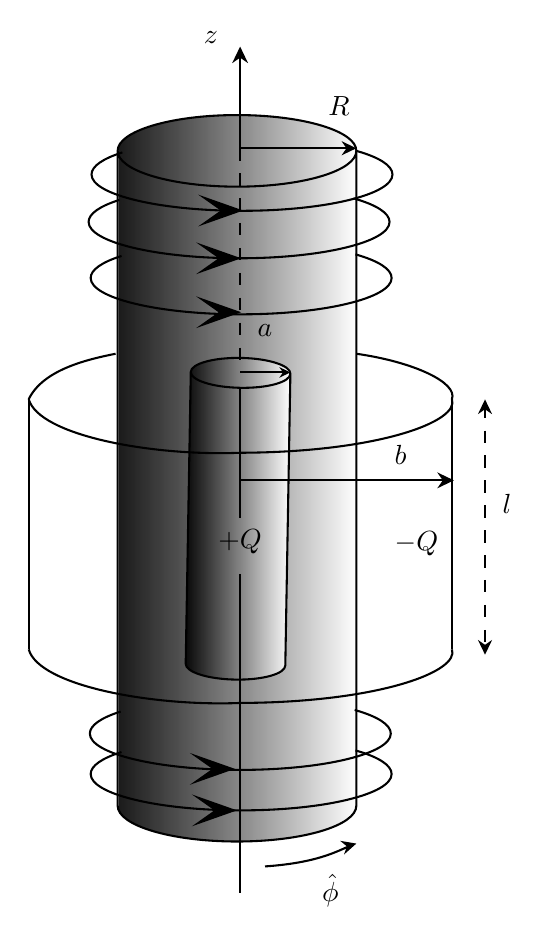
\begin{tikzpicture}[x=0.75pt,y=0.75pt,yscale=-1,xscale=1]
%uncomment if require: \path (0,509); %set diagram left start at 0, and has height of 509

%Shape: Can [id:dp09684604935566465] 
\path  [shading=_osh2e1ne2,_2z1s9o3hr,path fading= _xioe5epa2 ,fading transform={xshift=2}] (265,99.25) -- (265,414.75) .. controls (265,424.28) and (239.26,432) .. (207.5,432) .. controls (175.74,432) and (150,424.28) .. (150,414.75) -- (150,99.25) .. controls (150,89.72) and (175.74,82) .. (207.5,82) .. controls (239.26,82) and (265,89.72) .. (265,99.25) .. controls (265,108.78) and (239.26,116.5) .. (207.5,116.5) .. controls (175.74,116.5) and (150,108.78) .. (150,99.25) ; % for fading 
 \draw   (265,99.25) -- (265,414.75) .. controls (265,424.28) and (239.26,432) .. (207.5,432) .. controls (175.74,432) and (150,424.28) .. (150,414.75) -- (150,99.25) .. controls (150,89.72) and (175.74,82) .. (207.5,82) .. controls (239.26,82) and (265,89.72) .. (265,99.25) .. controls (265,108.78) and (239.26,116.5) .. (207.5,116.5) .. controls (175.74,116.5) and (150,108.78) .. (150,99.25) ; % for border 

%Shape: Can [id:dp5066897422779217] 
\path  [shading=_yc7cty2zc,_cw6yc9crn,path fading= _6up3sjiz1 ,fading transform={xshift=2}] (233.22,206.63) -- (230.77,347.21) .. controls (230.7,351.18) and (219.9,354.22) .. (206.65,353.99) .. controls (193.39,353.76) and (182.71,350.35) .. (182.78,346.37) -- (185.23,205.79) .. controls (185.3,201.82) and (196.1,198.78) .. (209.35,199.01) .. controls (222.61,199.24) and (233.29,202.65) .. (233.22,206.63) .. controls (233.15,210.61) and (222.35,213.64) .. (209.1,213.41) .. controls (195.85,213.18) and (185.16,209.77) .. (185.23,205.79) ; % for fading 
 \draw   (233.22,206.63) -- (230.77,347.21) .. controls (230.7,351.18) and (219.9,354.22) .. (206.65,353.99) .. controls (193.39,353.76) and (182.71,350.35) .. (182.78,346.37) -- (185.23,205.79) .. controls (185.3,201.82) and (196.1,198.78) .. (209.35,199.01) .. controls (222.61,199.24) and (233.29,202.65) .. (233.22,206.63) .. controls (233.15,210.61) and (222.35,213.64) .. (209.1,213.41) .. controls (195.85,213.18) and (185.16,209.77) .. (185.23,205.79) ; % for border 

%Straight Lines [id:da5767814872350512] 
\draw    (209,98) -- (209,52) ;
\draw [shift={(209,49)}, rotate = 450] [fill={rgb, 255:red, 0; green, 0; blue, 0 }  ][line width=0.08]  [draw opacity=0] (8.04,-3.86) -- (0,0) -- (8.04,3.86) -- (5.34,0) -- cycle    ;
%Straight Lines [id:da9586986950176424] 
\draw    (209.1,213.41) -- (209.1,276) ;
%Straight Lines [id:da13388264902555158] 
\draw    (209.1,303) -- (209.1,457) ;
%Straight Lines [id:da7507199722332254] 
\draw    (209,206) -- (230.22,206) ;
\draw [shift={(233.22,206)}, rotate = 180] [fill={rgb, 255:red, 0; green, 0; blue, 0 }  ][line width=0.08]  [draw opacity=0] (5.36,-2.57) -- (0,0) -- (5.36,2.57) -- (3.56,0) -- cycle    ;
%Straight Lines [id:da014240031855065727] 
\draw  [dash pattern={on 4.5pt off 4.5pt}]  (209,98) -- (209,205) ;
%Straight Lines [id:da07996399716506564] 
\draw    (209,98) -- (262,98) ;
\draw [shift={(265,98)}, rotate = 180] [fill={rgb, 255:red, 0; green, 0; blue, 0 }  ][line width=0.08]  [draw opacity=0] (7.14,-3.43) -- (0,0) -- (7.14,3.43) -- (4.74,0) -- cycle    ;
%Straight Lines [id:da7452678187994444] 
\draw    (107.15,218.88) -- (107.15,339.41) ;
%Straight Lines [id:da7334547584863753] 
\draw    (311.05,218.88) -- (311.05,339.41) ;
%Curve Lines [id:da21028021387310591] 
\draw    (107.15,339.41) .. controls (112,357) and (167,367) .. (209.1,365.24) ;
%Curve Lines [id:da0937851581321878] 
\draw    (107.15,218.88) .. controls (112,236.46) and (167,246.46) .. (209.1,244.7) ;
%Curve Lines [id:da652575597798738] 
\draw    (209.1,365.24) .. controls (276,365) and (315,350) .. (311.05,339.41) ;
%Curve Lines [id:da7826737740182319] 
\draw    (209.1,244.7) .. controls (276,244.46) and (315,229.46) .. (311.05,218.88) ;
%Curve Lines [id:da44822480153093114] 
\draw    (107.15,218.88) .. controls (114,205) and (134,200) .. (149,197) ;
%Curve Lines [id:da35663679232032575] 
\draw    (265,197) .. controls (293,201) and (314,211) .. (311.05,218.88) ;
%Shape: Arc [id:dp9829971486915707] 
\draw  [draw opacity=0] (263.59,122.12) .. controls (274.44,125.18) and (281,129.16) .. (281,133.5) .. controls (281,143.16) and (248.54,151) .. (208.5,151) .. controls (168.46,151) and (136,143.16) .. (136,133.5) .. controls (136,129.51) and (141.53,125.83) .. (150.85,122.89) -- (208.5,133.5) -- cycle ; \draw   (263.59,122.12) .. controls (274.44,125.18) and (281,129.16) .. (281,133.5) .. controls (281,143.16) and (248.54,151) .. (208.5,151) .. controls (168.46,151) and (136,143.16) .. (136,133.5) .. controls (136,129.51) and (141.53,125.83) .. (150.85,122.89) ;
%Shape: Arc [id:dp5086194350428808] 
\draw  [draw opacity=0] (264.59,149.12) .. controls (275.44,152.18) and (282,156.16) .. (282,160.5) .. controls (282,170.16) and (249.54,178) .. (209.5,178) .. controls (169.46,178) and (137,170.16) .. (137,160.5) .. controls (137,156.51) and (142.53,152.83) .. (151.85,149.89) -- (209.5,160.5) -- cycle ; \draw   (264.59,149.12) .. controls (275.44,152.18) and (282,156.16) .. (282,160.5) .. controls (282,170.16) and (249.54,178) .. (209.5,178) .. controls (169.46,178) and (137,170.16) .. (137,160.5) .. controls (137,156.51) and (142.53,152.83) .. (151.85,149.89) ;
%Shape: Arc [id:dp9528031588397792] 
\draw  [draw opacity=0] (265,99.25) .. controls (275.86,102.31) and (282.41,106.28) .. (282.41,110.63) .. controls (282.41,120.29) and (249.95,128.13) .. (209.91,128.13) .. controls (169.87,128.13) and (137.41,120.29) .. (137.41,110.63) .. controls (137.41,106.64) and (142.95,102.96) .. (152.26,100.02) -- (209.91,110.63) -- cycle ; \draw   (265,99.25) .. controls (275.86,102.31) and (282.41,106.28) .. (282.41,110.63) .. controls (282.41,120.29) and (249.95,128.13) .. (209.91,128.13) .. controls (169.87,128.13) and (137.41,120.29) .. (137.41,110.63) .. controls (137.41,106.64) and (142.95,102.96) .. (152.26,100.02) ;
%Shape: Arc [id:dp0406892088919768] 
\draw  [draw opacity=0] (264.59,388.12) .. controls (275.44,391.18) and (282,395.16) .. (282,399.5) .. controls (282,409.16) and (249.54,417) .. (209.5,417) .. controls (169.46,417) and (137,409.16) .. (137,399.5) .. controls (137,395.51) and (142.53,391.83) .. (151.85,388.89) -- (209.5,399.5) -- cycle ; \draw   (264.59,388.12) .. controls (275.44,391.18) and (282,395.16) .. (282,399.5) .. controls (282,409.16) and (249.54,417) .. (209.5,417) .. controls (169.46,417) and (137,409.16) .. (137,399.5) .. controls (137,395.51) and (142.53,391.83) .. (151.85,388.89) ;
%Shape: Arc [id:dp5418936946918034] 
\draw  [draw opacity=0] (264.19,368.62) .. controls (275.04,371.68) and (281.6,375.66) .. (281.6,380) .. controls (281.6,389.66) and (249.14,397.5) .. (209.1,397.5) .. controls (169.06,397.5) and (136.6,389.66) .. (136.6,380) .. controls (136.6,376.01) and (142.13,372.33) .. (151.45,369.39) -- (209.1,380) -- cycle ; \draw   (264.19,368.62) .. controls (275.04,371.68) and (281.6,375.66) .. (281.6,380) .. controls (281.6,389.66) and (249.14,397.5) .. (209.1,397.5) .. controls (169.06,397.5) and (136.6,389.66) .. (136.6,380) .. controls (136.6,376.01) and (142.13,372.33) .. (151.45,369.39) ;
\draw  [fill={rgb, 255:red, 0; green, 0; blue, 0 }  ,fill opacity=1 ] (192,122) -- (209,128) -- (192,134) -- (200.5,128) -- cycle ;
\draw  [fill={rgb, 255:red, 0; green, 0; blue, 0 }  ,fill opacity=1 ] (191,145) -- (208,151) -- (191,157) -- (199.5,151) -- cycle ;
\draw  [fill={rgb, 255:red, 0; green, 0; blue, 0 }  ,fill opacity=1 ] (191,171) -- (208,177) -- (191,183) -- (199.5,177) -- cycle ;
\draw  [fill={rgb, 255:red, 0; green, 0; blue, 0 }  ,fill opacity=1 ] (188,391) -- (205,397) -- (188,403) -- (196.5,397) -- cycle ;
\draw  [fill={rgb, 255:red, 0; green, 0; blue, 0 }  ,fill opacity=1 ] (189,411) -- (206,417) -- (189,423) -- (197.5,417) -- cycle ;
%Straight Lines [id:da5070443532226521] 
\draw    (209,258) -- (309,258) ;
\draw [shift={(312,258)}, rotate = 180] [fill={rgb, 255:red, 0; green, 0; blue, 0 }  ][line width=0.08]  [draw opacity=0] (8.04,-3.86) -- (0,0) -- (8.04,3.86) -- (5.34,0) -- cycle    ;
%Straight Lines [id:da5325651367585065] 
\draw  [dash pattern={on 4.5pt off 4.5pt}]  (327,222) -- (327,339) ;
\draw [shift={(327,342)}, rotate = 270] [fill={rgb, 255:red, 0; green, 0; blue, 0 }  ][line width=0.08]  [draw opacity=0] (7.14,-3.43) -- (0,0) -- (7.14,3.43) -- (4.74,0) -- cycle    ;
\draw [shift={(327,219)}, rotate = 90] [fill={rgb, 255:red, 0; green, 0; blue, 0 }  ][line width=0.08]  [draw opacity=0] (7.14,-3.43) -- (0,0) -- (7.14,3.43) -- (4.74,0) -- cycle    ;
%Curve Lines [id:da3233793317105156] 
\draw    (221,444) .. controls (246.38,442.25) and (255.67,436.67) .. (262.29,433.96) ;
\draw [shift={(265,433)}, rotate = 524.05] [fill={rgb, 255:red, 0; green, 0; blue, 0 }  ][line width=0.08]  [draw opacity=0] (7.14,-3.43) -- (0,0) -- (7.14,3.43) -- (4.74,0) -- cycle    ;

% Text Node
\draw (190,40.4) node [anchor=north west][inner sep=0.75pt]    {$z$};
% Text Node
\draw (250,71.4) node [anchor=north west][inner sep=0.75pt]    {$R$};
% Text Node
\draw (216,181.4) node [anchor=north west][inner sep=0.75pt]    {$a$};
% Text Node
\draw (282,239.4) node [anchor=north west][inner sep=0.75pt]    {$b$};
% Text Node
\draw (197,280.4) node [anchor=north west][inner sep=0.75pt]    {$+Q$};
% Text Node
\draw (282,281.4) node [anchor=north west][inner sep=0.75pt]    {$-Q$};
% Text Node
\draw (334,263.4) node [anchor=north west][inner sep=0.75pt]    {$l$};
% Text Node
\draw (247,446.4) node [anchor=north west][inner sep=0.75pt]    {$\hat{\phi }$};


\end{tikzpicture}

    \end{center}
    \begin{enumerate}[a)]
        \item \textbf{Vận tốc góc.}\\
        Khi dòng điện trong ống dây giảm dần tới không, các vỏ trụ bắt đầu quay. Hãy tính vận tốc góc (cả độ lớn và hướng) của hai vỏ trụ.
        \item \textbf{Nghịch lí Feynman.} \\
        Vì không có ngoại lực tác dụng lên hệ, moment động lượng (làm quay các vỏ trụ) ``xuất hiện''. Hãy phân tích một cách định lượng và chi tiết nghịch lí này.
        \item \textbf{Nan hoa.} \\
        Bây giờ thay vì cho dòng điện trong ống dây giảm dần, ta nối cứng hai vỏ trụ với nhau bằng một nan hoa theo phương bán kính có khối lượng không đáng kể. Biết rằng nan hoa có độ dẫn điện nhỏ để có thể bỏ qua dòng điện dịch. Hãy xác định moment động lượng toàn phần của hai vỏ trụ trong trường hợp này cũng như vận tốc góc của nó.
    \end{enumerate}
\end{enumerate}

\end{vd}
\begin{loigiai}
    

\begin{enumerate}[1)]
    \item Vì sóng điện từ có thể coi là được tạo ra từ các photon, nên động lượng của chúng là:
$$\delta p=\dfrac{\delta W}{c}=\dfrac{S\delta A \delta t}{c},$$
với $c$ là tốc độ ánh sáng trong chân không. Từ đó suy ra mật độ động lượng:
$$p_v=\dfrac{\delta p}{\delta V}=\dfrac{S \delta A \delta t}{c\delta A \delta l}=\dfrac{S}{c\dfrac{\delta l}{\delta t}}=\dfrac{S}{c^2}.$$
Biểu diễn dưới dạng vector:
$$\ot{p_v}=\dfrac{1}{\mu_0 c^2}\ot{E}\times\ot{B}.$$
    \item \textbf{Nghịch lí Feynman.}
    \begin{enumerate}[a)]
        \item \textbf{Vận tốc góc.}\\
        Dòng điện chạy qua ống solenoid tạo ra một từ trường bên trong nó:
        $$\ot{B}=\mu_0 ni\hat{z} \quad (r<R).$$
        Khi cường độ dòng điện giảm thì cảm ứng từ giảm, làm xuất hiện điện trường xoáy (có đường sức điện tròn), theo định luật Faraday:
        $$\ot{E}.2\pi r \hat{\phi}=-\dfrac{\mathrm{d}}{\mathrm{d}t}\tron{\ot{B}\cdot\ot{S}}.$$
        Nếu $r<R$ thì $\ot{S}=\pi r^2 \hat{z}$ và
        $$\ot{E}=-\dfrac{1}{2}\mu_0 n\dfrac{\mathrm{d}i}{\mathrm{d}t}r\hat{\phi},$$
        còn nếu $r>R$, thì $\ot{S}=\pi R^2 \hat{z}$ và
         $$\ot{E}=-\dfrac{1}{2}\mu_0 n\dfrac{\mathrm{d}i}{\mathrm{d}t}\dfrac{R^2}{r}\hat{\phi}.$$
         Moment lực đối với vỏ trụ bên trong là: 
         $$\ot{\tau_a}=\ot{r} \times Q \ot{E}=-\frac{1}{2} \mu_{0} n Q a^{2} \frac{\dd i}{\dd t} \hat{r} \times \hat{\phi}=-\frac{1}{2} \mu_{0} n Q a^{2} \frac{\dd i}{\dd t} \hat{z}.$$
         Theo định lí biến thiên moment động lượng:
         $$\ot{\tau_a}=\dfrac{\mathrm{d}\ot{L_a}}{\mathrm{d}t},$$
         suy ra, 
         $$\Delta \ot{L_a}=-\dfrac{1}{2}\mu_0 n Q a^2 \Delta i \hat{z},$$
         hay
         $$\ot{L_a}=\dfrac{1}{2}\mu_0 n Q a^2 i \hat{z}.$$
         Ta có:
         $$\ot{L_a}=I\ot{\omega_a}=m_a a^2\ot{\omega_a}=2\pi l \sigma a^3 \ot{\omega_a},$$
         suy ra
         $$\ot{\omega_a}=\dfrac{\mu_0 nQi}{4\pi l\sigma a}\hat{z}.$$
         Tương tự, moment lực đối với vỏ trụ bên ngoài:
         $$\ot{\tau}_{b}=\ot{r} \times (-Q) \ot{E}=\frac{1}{2} \mu_{0} n Q R^{2} \frac{\dd i}{\dd t} \hat{r} \times \hat{\phi}=\frac{1}{2} \mu_{0} n Q R^{2} \frac{\dd i}{\dd t} \hat{z}.$$
         Sử dụng định lí biến thiên moment động lượng:
         $$\ot{\tau_b}=\dfrac{\mathrm{d}\ot{L_b}}{\mathrm{d}t},$$
         độ biến thiên moment động lượng được tính bởi
         $$\Delta \ot{L_b}=\dfrac{1}{2}\mu_0 n Q R^2 \Delta i \hat{z},$$
         hay
         $$\ot{L_b}=-\dfrac{1}{2}\mu_0 n Q R^2 i \hat{z}.$$
         Vì
          $$\ot{L_b}=I\ot{\omega_b}=m_b b^2\ot{\omega_b}=2\pi l \sigma b^3 \ot{\omega_b},$$
         nên
         $$\ot{\omega_b}=\dfrac{\mu_0 nQiR^2}{4\pi l\sigma b^3}\hat{z},$$
        điều này có nghĩa rằng vỏ trụ ngoài xoay theo chiều kim đồng hồ khi ta nhìn từ trên xuống.
        \item \textbf{Nghịch lí Feynman.}\\
        Ở vùng không gian ở giữa hai vỏ trụ $(a<r<b)$ có một điện trường với cường độ được xác định bởi định luật Gauss:
        $$\ot{E}=\dfrac{Q}{2\pi\varepsilon_0 l}\dfrac{1}{r}\hat{r}.$$
        Vì có dòng điện chạy trong ống solenoid nên bên trong nó cũng xuất hiện từ trường, mật độ động lượng của trường điện từ là:
        $$\ot{p_v}=\varepsilon_{0} \ot{E} \times \ot{B}=\frac{Q}{2 \pi l} \frac{1}{r} \hat{r} \times \mu_{0} n i \hat{z}=-\frac{\mu_{0} n i Q}{2 \pi l} \frac{1}{r} \hat{\phi}.$$
        Mật độ moment động lượng của trường điện từ là:
        $$\ot{l_{\text{em}}}=\ot{r} \times \ot{p_v}=-\frac{\mu_{0} n i Q}{2 \pi l} \hat{r} \times \hat{\phi}=-\frac{\mu_{0} n i Q}{2 \pi l} \hat{z}.$$
        Vậy moment động lượng là:
        $$\ot{L_{\text{em}}}=\ot{l_{\text{em}}} \times \pi\left(R^{2}-a^{2}\right) l=-\frac{1}{2} \mu_{0} n i Q\left(R^{2}-a^{2}\right) \hat{z}.$$
        Dựa vào kết quả trên, có thể dễ dàng thấy:
        $$\ot{L_{\text{em}}}=\ot{L_a}+\ot{L_b},$$
        tức là moment động lượng của trường điện từ biến đổi hoàn toàn thành moment động lượng cơ học (làm quay các vỏ trụ).
        \item \textbf{Nan hoa.} \\
        Trường hợp này không còn điện trường nên cơ chế biến thiên moment động lượng sẽ phụ thuộc vào lực Lorentz. Vì vậy, lực tác dụng lên một đoạn
        $\mathrm{d}\ot{r}=\mathrm{d}r\hat{r}$ của nan hoa là:
        $$d \ot{F}=i_1 d \ot{r} \times \ot{B}=i_1 B d r \hat{r} \times \hat{z}=i_{1} B d r(-\hat{\phi})=-i_{1} B d r \hat{\phi},$$
        trong đó $i_1=\dfrac{\dd Q}{\dd t},$ là dòng điện có hướng đi ra khỏi các vỏ trụ và
        $$ \ot{B}=\left\{ \begin{aligned}
        \mu_0 n i \hat{z},& \text { với } a<r<R, \\
        \overrightarrow{0}, &\text { với } r>R,
        \end{aligned}\right.$$
        là từ trường do ống solenoid tạo ra.\\
        Moment lực đối với nan hoa là:
        $$\ot{\tau}=\int_{a}^{b} \ot{r} \times d \ot{F}=-\mu_0 n i i_{1}\left(\int_{a}^{R} r d r\right) \hat{r} \times \hat{\phi}=-\frac{1}{2} \mu_{0} n i i_1\left(R^{2}-a^{2}\right) \hat{z}.$$
        Vì $\ot{\tau}=\dfrac{\dd \ot{L}}{\dd t},$ nên 
        $$\dfrac{\dd \ot{L}}{\dd t}=-\dfrac{1}{2} \mu_0 n i \dfrac{\dd Q}{\dd t}\left(R^{2}-a^{2}\right) \hat{z},$$
        hay
        $$\Delta\ot{L}=-\dfrac{1}{2} \mu_0 n i  \Delta Q  \left(R^{2}-a^{2}\right) \hat{z}.$$
        Ta lại có:
        $$\Delta\ot{L}=\ot{L}-\ot{0}=\ot{L} \text{ và } \Delta Q=Q-0=Q,$$
        suy ra
        $$\ot{L}=-\dfrac{1}{2} \mu_0 n i  Q  \left(R^{2}-a^{2}\right) \hat{z},$$
        phù hợp với kết quả về moment động lượng của trường điện từ.\\
        Cuối cùng, vận tốc góc của các vỏ trụ là:
        $$\ot{\omega}=\frac{\ot{L}}{I_{\text{tổng}}}=-\frac{\mu_{0} n i Q\left(R^{2}-a^{2}\right)}{4 \pi \sigma l\left(a^{3}+b^{3}\right)} \hat{z} .$$
    \end{enumerate}
\end{enumerate}
\end{loigiai}


\begin{vd}[Máy gia tốc proton]
Đại học Beloit có một máy gia tốc proton $500 ~\mathrm{kV}$ VanDeGraff ``tự chế'', được thiết kế và chế tạo bởi các sinh viên và giảng viên.
\begin{center}
    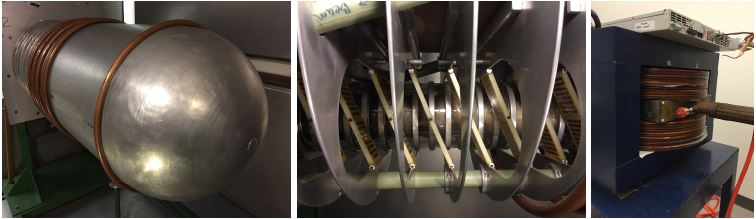
\includegraphics[scale=0.65]{Anh/ngoc3.JPG}
\end{center}
    Các hình trên lần lượt là mái vòm của máy gia tốc (giả thiết rằng nó hình cầu), cột gia tốc và nam châm điện.\\

Vòm của máy gia tốc là một quả cầu nhôm có bán kính $a=0,5~\mathrm{m}$, được tích điện bởi một sợi dây cao su có bề rộng $w=10~\mathrm{cm}$ chuyển động với tốc độ $v_b=20~\mathrm{m/s}$. Cột gia tốc bao gồm $20$ vòng kim loại ngăn cách với nhau bởi các vòng thủy tinh; các vòng mắc nối tiếp với điện trở $500~\mathrm{M}\Omega$. Chùm proton với cường độ dòng điện $25~\mu \mathrm{A}$ và được gia tốc bởi điện thế $500~\mathrm{kV}$ rồi sau đó đi qua một nam châm điện hiệu chỉnh. Nam châm điện gồm các vòng dây dẫn bằng đồng, có tác dụng tạo ra từ trường đều $B$ bên trong một vùng có bán kính $b=10~\mathrm{cm}$ và từ trường bằng không bên ngoài vùng không gian đó.
\begin{center}
 

\tikzset{every picture/.style={line width=0.75pt}} %set default line width to 0.75pt        

\begin{tikzpicture}[x=0.75pt,y=0.75pt,yscale=-1,xscale=1]
%uncomment if require: \path (0,543); %set diagram left start at 0, and has height of 543

%Shape: Rectangle [id:dp2756080105813059] 
\draw  [draw opacity=0][fill={rgb, 255:red, 155; green, 155; blue, 155 }  ,fill opacity=0.33 ] (131.67,333.36) .. controls (131.67,330.6) and (133.91,328.36) .. (136.67,328.36) -- (448.09,328.36) .. controls (450.85,328.36) and (453.09,330.6) .. (453.09,333.36) -- (453.09,338.59) .. controls (453.09,341.36) and (450.85,343.59) .. (448.09,343.59) -- (136.67,343.59) .. controls (133.91,343.59) and (131.67,341.36) .. (131.67,338.59) -- cycle ;
%Shape: Ellipse [id:dp1631084327669441] 
\draw  [line width=2.25]  (75,336.88) .. controls (75,305.46) and (101.41,279.99) .. (133.99,279.99) .. controls (166.57,279.99) and (192.98,305.46) .. (192.98,336.88) .. controls (192.98,368.3) and (166.57,393.77) .. (133.99,393.77) .. controls (101.41,393.77) and (75,368.3) .. (75,336.88) -- cycle ;
%Shape: Ellipse [id:dp28020169257841254] 
\draw  [line width=2.25]  (419.41,336.88) .. controls (419.41,318.69) and (434.7,303.95) .. (453.55,303.95) .. controls (472.41,303.95) and (487.69,318.69) .. (487.69,336.88) .. controls (487.69,355.06) and (472.41,369.8) .. (453.55,369.8) .. controls (434.7,369.8) and (419.41,355.06) .. (419.41,336.88) -- cycle ;
%Straight Lines [id:da02664344415842912] 
\draw    (185.55,309.55) -- (433.58,309.55) ;
%Straight Lines [id:da9047525706494886] 
\draw    (187.4,361.51) -- (429.86,361.51) ;
%Straight Lines [id:da22782514761826667] 
\draw [line width=5.25]    (205.05,302.38) -- (205.05,369.58) ;
%Straight Lines [id:da5683744309061505] 
\draw [line width=5.25]    (245.93,302.38) -- (245.93,369.58) ;
%Straight Lines [id:da4574514472799318] 
\draw [line width=5.25]    (327.68,303.28) -- (327.68,370.47) ;
%Straight Lines [id:da5882533127674177] 
\draw [line width=5.25]    (286.8,302.38) -- (286.8,369.58) ;
%Straight Lines [id:da8171609876395312] 
\draw [line width=5.25]    (366.69,302.38) -- (366.69,369.58) ;
%Straight Lines [id:da9743756944485404] 
\draw [line width=5.25]    (405.71,302.38) -- (405.71,369.58) ;
%Straight Lines [id:da9507626123465847] 
\draw    (205.05,369.58) -- (205.05,414.37) ;
%Straight Lines [id:da7718584311897159] 
\draw    (286.8,369.58) -- (286.8,414.37) ;
%Straight Lines [id:da034921198175972945] 
\draw    (245.93,369.58) -- (245.93,414.37) ;
%Straight Lines [id:da9862567414878582] 
\draw    (405.71,369.58) -- (405.71,413.48) ;
%Straight Lines [id:da4116211672875447] 
\draw    (366.69,369.58) -- (366.69,414.37) ;
%Straight Lines [id:da5665810127110102] 
\draw    (327.68,370.47) -- (327.68,415.27) ;
%Straight Lines [id:da1381103821044758] 
\draw    (162.32,386.6) -- (172.54,413.48) ;
%Shape: Resistor [id:dp7361645764419116] 
\draw   (172.54,413.48) -- (178.56,413.48) -- (179.9,404.52) -- (182.57,422.43) -- (185.25,404.52) -- (187.92,422.43) -- (190.6,404.52) -- (193.28,422.43) -- (195.95,404.52) -- (198.63,422.43) -- (199.96,413.48) -- (205.98,413.48) ;
%Shape: Resistor [id:dp34785780596395166] 
\draw   (205.98,413.48) -- (213.17,413.48) -- (214.77,404.07) -- (217.97,422.88) -- (221.16,404.07) -- (224.36,422.88) -- (227.55,404.07) -- (230.75,422.88) -- (233.95,404.07) -- (237.14,422.88) -- (238.74,413.48) -- (245.93,413.48) ;
%Shape: Resistor [id:dp9054517758554483] 
\draw   (285.87,413.48) -- (293.4,413.48) -- (295.07,404.07) -- (298.42,422.88) -- (301.76,404.07) -- (305.1,422.88) -- (308.45,404.07) -- (311.79,422.88) -- (315.14,404.07) -- (318.48,422.88) -- (320.15,413.48) -- (327.68,413.48) ;
%Shape: Resistor [id:dp9382728705904546] 
\draw   (245.93,413.48) -- (253.12,413.48) -- (254.72,404.07) -- (257.91,422.88) -- (261.11,404.07) -- (264.3,422.88) -- (267.5,404.07) -- (270.7,422.88) -- (273.89,404.07) -- (277.09,422.88) -- (278.68,413.48) -- (285.87,413.48) ;
%Shape: Resistor [id:dp4186647519609439] 
\draw   (367.62,413.48) -- (374.48,413.48) -- (376,404.07) -- (379.05,422.88) -- (382.1,404.07) -- (385.14,422.88) -- (388.19,404.07) -- (391.24,422.88) -- (394.28,404.07) -- (397.33,422.88) -- (398.85,413.48) -- (405.71,413.48) ;
%Shape: Resistor [id:dp4913409831205102] 
\draw   (327.68,413.48) -- (334.87,413.48) -- (336.47,404.07) -- (339.66,422.88) -- (342.86,404.07) -- (346.05,422.88) -- (349.25,404.07) -- (352.44,422.88) -- (355.64,404.07) -- (358.83,422.88) -- (360.43,413.48) -- (367.62,413.48) ;
%Straight Lines [id:da5932831172912454] 
\draw    (205.05,236.09) -- (205.05,294.9) ;
\draw [shift={(205.05,297.9)}, rotate = 270] [fill={rgb, 255:red, 0; green, 0; blue, 0 }  ][line width=0.08]  [draw opacity=0] (8.04,-3.86) -- (0,0) -- (8.04,3.86) -- (5.34,0) -- cycle    ;
%Straight Lines [id:da017143479683142893] 
\draw    (205.05,236.09) -- (245.18,295.42) ;
\draw [shift={(246.86,297.9)}, rotate = 235.93] [fill={rgb, 255:red, 0; green, 0; blue, 0 }  ][line width=0.08]  [draw opacity=0] (8.04,-3.86) -- (0,0) -- (8.04,3.86) -- (5.34,0) -- cycle    ;
%Straight Lines [id:da27951023916710005] 
\draw    (205.05,236.09) -- (283.48,295.2) ;
\draw [shift={(285.87,297.01)}, rotate = 217.01] [fill={rgb, 255:red, 0; green, 0; blue, 0 }  ][line width=0.08]  [draw opacity=0] (8.04,-3.86) -- (0,0) -- (8.04,3.86) -- (5.34,0) -- cycle    ;
%Straight Lines [id:da1974640420582534] 
\draw    (351.83,277.3) -- (309.83,301.77) ;
\draw [shift={(307.24,303.28)}, rotate = 329.77] [fill={rgb, 255:red, 0; green, 0; blue, 0 }  ][line width=0.08]  [draw opacity=0] (8.04,-3.86) -- (0,0) -- (8.04,3.86) -- (5.34,0) -- cycle    ;
%Straight Lines [id:da9907676201388216] 
\draw    (351.83,277.3) -- (346.03,301.26) ;
\draw [shift={(345.33,304.17)}, rotate = 283.6] [fill={rgb, 255:red, 0; green, 0; blue, 0 }  ][line width=0.08]  [draw opacity=0] (8.04,-3.86) -- (0,0) -- (8.04,3.86) -- (5.34,0) -- cycle    ;
%Straight Lines [id:da817099320829259] 
\draw    (351.83,277.3) -- (383.87,303.19) ;
\draw [shift={(386.2,305.07)}, rotate = 218.94] [fill={rgb, 255:red, 0; green, 0; blue, 0 }  ][line width=0.08]  [draw opacity=0] (8.04,-3.86) -- (0,0) -- (8.04,3.86) -- (5.34,0) -- cycle    ;
%Straight Lines [id:da8351175753738009] 
\draw    (351.83,277.3) -- (422.41,304.01) ;
\draw [shift={(425.22,305.07)}, rotate = 200.73] [fill={rgb, 255:red, 0; green, 0; blue, 0 }  ][line width=0.08]  [draw opacity=0] (8.04,-3.86) -- (0,0) -- (8.04,3.86) -- (5.34,0) -- cycle    ;
%Straight Lines [id:da19294180977800623] 
\draw    (429.86,413.48) -- (405.71,413.48) ;
%Straight Lines [id:da4408218359878966] 
\draw    (429.86,413.48) -- (429.86,428.71) ;
%Straight Lines [id:da9048890648918955] 
\draw    (412.68,428.71) -- (447.05,428.71) ;
%Straight Lines [id:da8284802750722475] 
\draw    (419.64,434.08) -- (441.94,434.08) ;
%Straight Lines [id:da5994834503037612] 
\draw    (424.29,439.46) -- (439.15,439.46) ;
%Shape: Rectangle [id:dp7377878361139141] 
\draw  [draw opacity=0][fill={rgb, 255:red, 155; green, 155; blue, 155 }  ,fill opacity=0.33 ] (450.47,332.63) .. controls (451.92,330.27) and (455.03,329.47) .. (457.43,330.84) -- (555.33,386.75) .. controls (557.73,388.12) and (558.5,391.14) .. (557.05,393.5) -- (555.1,396.67) .. controls (553.66,399.02) and (550.54,399.82) .. (548.14,398.45) -- (450.24,342.54) .. controls (447.85,341.18) and (447.08,338.16) .. (448.52,335.8) -- cycle ;
%Straight Lines [id:da8116605181148742] 
\draw [line width=1.5]    (487.46,343.59) -- (564.56,387.49) ;
%Straight Lines [id:da41090489651557305] 
\draw [line width=1.5]    (477.24,362.41) -- (554.34,406.31) ;
%Straight Lines [id:da20427698767667568] 
\draw [line width=1.5]    (564.56,387.49) -- (554.34,406.31) ;

% Text Node
\draw (74.76,255.26) node [anchor=north west][inner sep=0.75pt]    {$\text{Mái vòm}$};
% Text Node
\draw (128.46,212.26) node [anchor=north west][inner sep=0.75pt]    {$\text{Các vòng kim loại của cột gia tốc}$};
% Text Node
\draw (299.05,253.47) node [anchor=north west][inner sep=0.75pt]    {$\text{Các vòng thủy tinh}$};
% Text Node
\draw (480.87,288.41) node [anchor=north west][inner sep=0.75pt]    {$\text{Nam châm điện}$};
% Text Node
\draw (235.98,433.54) node [anchor=north west][inner sep=0.75pt]    {$\text{Chuỗi điện trở}$};
% Text Node
\draw (521.59,414.73) node [anchor=north west][inner sep=0.75pt]    {$\text{Mục tiêu}$};
\end{tikzpicture}

\end{center}

    Chỉ có $6$ trong tổng số $20$ vòng kim loại và điện trở được thể hiện trong hình. Phần hình vẽ màu xám mờ là con đường mà proton thực hiện khi được tăng tốc từ máy vòm, thông qua nam châm điện để đến được mục tiêu.

\begin{enumerate}[1)]
    \item Giả sử mái vòm được tích điện đến $500 ~\mathrm{kV}$, hãy xác định cường độ điện trường trên bề mặt của mái vòm.
    \item Giả sử rằng chùm tia proton được tắt, tìm hằng số thời gian của mái vòm (thời gian để điện tích trên mái vòm giảm còn $1/e\approx1/3$ giá trị ban đầu.
    \item Giả sử rằng chùm proton $25 ~\mu \mathrm{A}$ được bật, xác định mật độ điện tích bề mặt cần phải phun lên dây đai để duy trì điện thế $500~\mathrm{kV}$ ổn định trên vòm.
    \item Chùm proton đi vào nam châm điện và bị lệch một góc $\theta=10^\circ$. Xác định độ lớn của cảm ứng từ.
    \begin{center}
\tikzset{every picture/.style={line width=0.75pt}} %set default line width to 0.75pt        

\begin{tikzpicture}[x=0.75pt,y=0.75pt,yscale=-1,xscale=1]
%uncomment if require: \path (0,300); %set diagram left start at 0, and has height of 300

%Shape: Circle [id:dp769233356039938] 
\draw  [line width=1.5]  (91,125.5) .. controls (91,93.19) and (117.19,67) .. (149.5,67) .. controls (181.81,67) and (208,93.19) .. (208,125.5) .. controls (208,157.81) and (181.81,184) .. (149.5,184) .. controls (117.19,184) and (91,157.81) .. (91,125.5) -- cycle ;
%Straight Lines [id:da7844220980663261] 
\draw  [dash pattern={on 4.5pt off 4.5pt}]  (43,125.5) -- (272,125.5) ;
%Straight Lines [id:da5098925486608799] 
\draw [line width=3]    (33,125.5) -- (91,125.5) ;
%Curve Lines [id:da380068325407648] 
\draw [line width=3]    (91,125.5) .. controls (139,129) and (157,141) .. (186,170) ;
%Straight Lines [id:da9258517733136686] 
\draw [line width=3]    (186,170) -- (241.76,225.76) ;
\draw [shift={(246,230)}, rotate = 225] [fill={rgb, 255:red, 0; green, 0; blue, 0 }  ][line width=0.08]  [draw opacity=0] (18.75,-9.01) -- (0,0) -- (18.75,9.01) -- (12.45,0) -- cycle    ;
%Curve Lines [id:da04614005683561362] 
\draw    (197.88,173.21) .. controls (218.82,159.66) and (219.11,147.48) .. (220.73,129.83) ;
\draw [shift={(221,127)}, rotate = 455.71] [fill={rgb, 255:red, 0; green, 0; blue, 0 }  ][line width=0.08]  [draw opacity=0] (7.14,-3.43) -- (0,0) -- (7.14,3.43) -- (4.74,0) -- cycle    ;
\draw [shift={(195,175)}, rotate = 329.04] [fill={rgb, 255:red, 0; green, 0; blue, 0 }  ][line width=0.08]  [draw opacity=0] (7.14,-3.43) -- (0,0) -- (7.14,3.43) -- (4.74,0) -- cycle    ;
%Straight Lines [id:da683950270522611] 
\draw  [dash pattern={on 4.5pt off 4.5pt}]  (149.5,125.5) -- (185,165) ;

% Text Node
\draw (228,146.4) node [anchor=north west][inner sep=0.75pt]    {$\theta $};
% Text Node
\draw (200,245.4) node [anchor=north west][inner sep=0.75pt]    {$\text{Hướng đi của proton}$};
% Text Node
\draw (104,34.4) node [anchor=north west][inner sep=0.75pt]    {$\text{Nam châm điện}$};
\end{tikzpicture}

    \end{center}
    \item Nam châm điện được cấu tạo bởi các lớp dây đồng cuốn xoắn ốc, dây có đường kính trong $d_i=0,40~\mathrm{cm}$ và đường kính ngoài $d_o=0,50~\mathrm{cm}$. Hình xoắn ốc phẳng tạo thành bởi các dây đồng có đường kính trong $D_i=20~\mathrm{cm}$ và đường kính ngoài $D_0=50~\mathrm{cm}$. Giả sử các cuộn dây được cuốn sát nhau, xác định chiều dài dây $L$ của một xoắn ốc.
    \begin{center}
        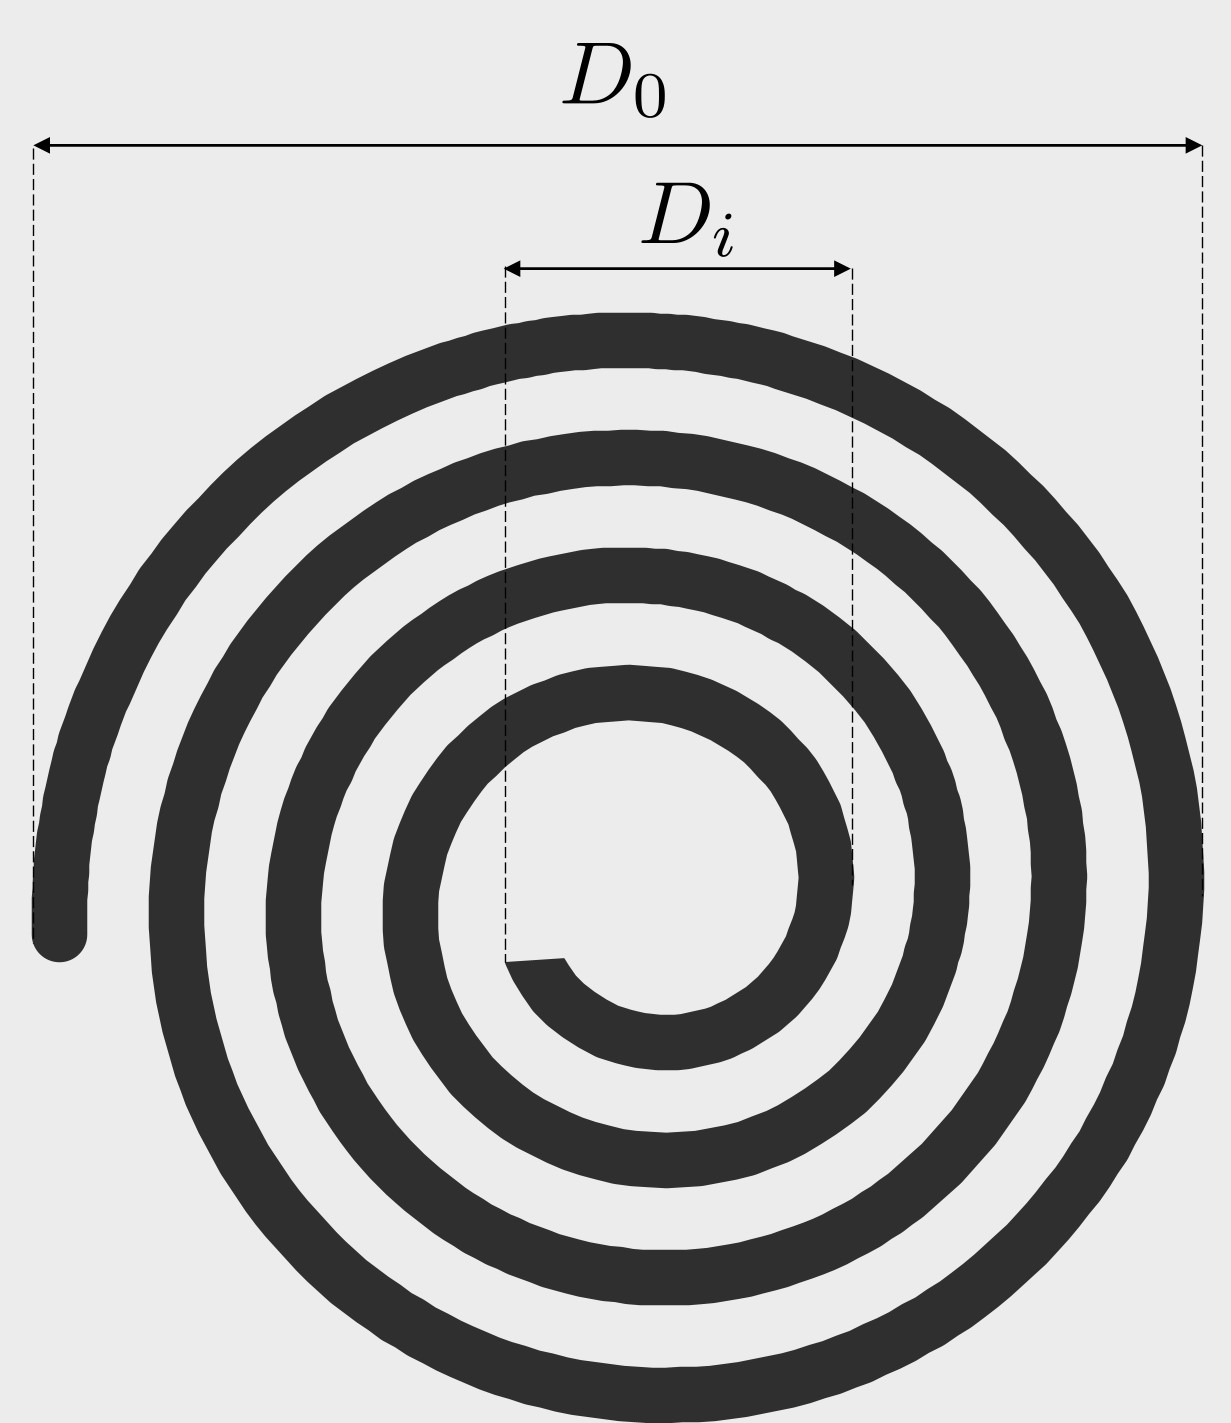
\includegraphics[scale=0.4]{Anh/xoanoc.jpg}
    \end{center}
    \item Ống rỗng được sử dụng để thay cho các sợi dây dẫn rắn giúp làm mát nam châm. Nếu điện trở suất của đồng là $\rho=1,7\times10^{-8}~\Omega\cdot \mathrm{m}$, hãy xác định điện trở của một vòng xoắn ốc.
    \item Có $N=24$ cuộn dây xếp chồng lên nhau. Nước máy với nhiệt độ ban đầu $T_c=18^\circ \mathrm{C}$ đi vào vòng xoắn thông qua ống đồng để ngăn nó nóng lên, nước đi ra với nhiệt độ $T_j=31^\circ \mathrm{C}$. Ống đồng có dòng điện $45 ~\mathrm{A}$ nhằm tạo ra từ trường cần thiết. Cần phải cung cấp nước làm mát với tốc độ bao nhiêu cho nam châm điện? Biểu diễn kết quả với đơn vị lít trên giây và chỉ bao gồm một chữ số có nghĩa. Biết nhiệt dung riêng của nước là $4200~\mathrm{J/^\circ C\cdot kg}$; khối lượng riêng của nước là $1000 ~\mathrm{kg/m^3}$.
    \item Các proton được bắn vào một mục tiêu gồm các nguyên từ Flo $\tron{Z=9}$. Khoảng cách gần nhất tới tâm của nguyên tử Flo mà các proton tiếp cận được là bao nhiêu? Có thể giả sử rằng nguyên tử Flo không chuyển động.
\end{enumerate}
\end{vd}
\begin{loigiai}
    

\begin{enumerate}[1)]
    \item Ta có biểu thức điện thế
    $$ V=\dfrac{q}{4\pi\varepsilon_0a},$$
    và cường độ điện trường là:
    $$E=\dfrac{q}{4\pi\varepsilon_0a^2},$$
    do đó:
    $$E=\dfrac{V}{a}=10^6 ~\mathrm{V/m}.$$
    \item Hằng số thời gian: $\tau=RC,$ trong đó
    $$C=Q/V=4\pi\varepsilon_0a=5,56\times10^{-11}~\mathrm{F},$$
    và 
    $$R=20r_0=10^{10}~\Omega.$$
    nên 
    $$\tau=RC=0,556~\mathrm{s}.$$
    \item Có nhiều cách để mái vòm phóng điện, hai trong số đó là thông qua điện trở và chùm proton. Chúng ta sẽ chỉ xét hai cách này.
    Ở $500~\mathrm{kV}$, dòng điện chạy qua chuỗi điện trở là $50~\mu \mathrm{A}$, từ $V=IR$. Do đó tổng dòng điện $I$ cần cung cấp cho mái vòm là $75~\mu \mathrm{A}$. Dòng điện này được phun lên dây đai với tốc độ là:
    $$\dfrac{\delta A}{\Delta t}=v_bw,$$
    do đó mật độ điện tích mặt cần thiết là:
    $$\sigma=\dfrac{I}{v_bw}=\dfrac{\tron{75~\mu\mathrm{ C/s}}}{\tron{20~\mathrm{m/s}}\tron{0.10~\mathrm{m}}}=37,5~\mu \mathrm{C/m^2}.$$
    \item Bắt đầu từ biểu thức $F=qvB$ trong đó $F$ là lực tác dụng lên các proton, và $v$ là vận tốc của chúng. Các proton phi tương đối tính, nên
    $$\dfrac{1}{2}mv^2=qV.$$
    Chúng chuyển động trong vòng tròn bán kính $r$ bên trong từ trường, ta có:
    $$\dfrac{mv^2}{r}=qvB.$$
    Kết hợp hai phương trình trên ta được:
    $$r=\dfrac{mv}{qB}=\dfrac{m}{qB}\sqrt{\dfrac{2qV}{m}}=\dfrac{1}{B}\sqrt{\dfrac{2mV}{q}}.$$
    Vậy độ lớn cảm ứng từ là:
    $$B=\dfrac{1}{4}\sqrt{\dfrac{2mV}{q}}.$$
    Để liên hệ cảm ứng từ với góc, ta cần thực hiện một số công việc hình học. Vẽ hai vòng tròn, một với bán kính $b$, một với bán kính $r$, trên cùng một mặt phẳng và cắt nhau như hình vẽ ở đề bài. Khi đó vẽ một hình tam giác ta được:
    $$\tan \dfrac{\theta}{2}=\dfrac{b}{r}.$$
    Kết hợp các phương trình, kết quả là
    $$B=\dfrac{\tan \theta/2}{b}\sqrt{\dfrac{2mV}{q}}=0,0894 ~\mathrm{T}.$$
    \item Diện tích của hình xoắn ốc là
    $$A=\dfrac{\pi}{4}\tron{D_0^2-D_i^2}.$$
    Diện tích của phần dây được vẽ trên hình là:
    $$A=Ld_0.$$
    Cân bằng hai phương trình, giải ra ta được:
    $$L=\dfrac{\pi\tron{D_0^2-D_i^2}}{4d_0}=33~\mathrm{m}.$$
    \item Ta có
    $$r_s=\dfrac{\rho L}{A},$$
    trong đó $A$ là diện tích mặt cắt của dây, hay
    $$A=\dfrac{\pi}{4}\tron{d_0^2-d_i^2}=7.1\times10^{-6}~\mathrm{m^2}.$$
    Kết hợp, ta được:
    $$r_s=\dfrac{\rho}{d_0}\dfrac{D_0^2-D_i^2}{d_0^2-d_i^2}=0.079~\Omega.$$
    \item Tốc độ sinh nhiệt trong các cuộn dây là:
    $$P=I^2R=I^2Nr_s=3850~\mathrm{W}.$$
    Điều này được giảm bớt thông qua việc tăng nhiệt độ của nước:
    $$P=C\Delta Tq,$$
    trong đó $C$ là nhiệt dung riêng tính bằng lít và $Q$ là tốc độ chảy tính bằng lít trên giây. Vì một lít nước nặng $1~\mathrm{kg}$ nên ta có thể sử dụng $C$. Kết hợp các phương tình ta được:
    $$Q=\dfrac{I^2Nr}{C\Delta T}=0.07~\mathrm{l/s}.$$
    \item Bảo toàn năng lượng ta được:
    $$qV=\dfrac{1}{4\pi\varepsilon_0}\dfrac{Zq^2}{r},$$
    trong đó $r$ là khoảng tiếp cận gần nhất. Khi đó:
    $$r=\dfrac{1}{4\pi\varepsilon_0}\dfrac{Zq}{V}=2.59\times 10^{-14}~\mathrm{m}.$$
    Vì kết quả này bằng với kích thước của một hạt nhân Flo, có thể sẽ xảy ra một phản ứng hạt nhân. Trên thực tế, phản ứng sẽ xảy ra ở khoảng $380~\mathrm{kV}$.
    
\end{enumerate}
\end{loigiai}


\begin{vd}[Hiện tượng từ trễ và khử từ]
%\textbf{Bài 3 IZho 2015}
Trong bài toán này, bỏ qua tốc độ lan truyền của sự tương tác điện từ.
\begin{center}
\textbf{Phần I: Nam châm}
\end{center}
\begin{enumerate}[1)]
\item \textbf{Giới thiệu lí thuyết:}\\
Ở khoảng cách rất lớn, từ trường được tạo ra bởi sự từ hóa đồng nhất trên một trụ sắt từ (nam châm vĩnh cửu) tương đương với trường tạo ra bởi một cuộn dây tròn có dòng điện không đổi.\\
\begin{center}
    

% Gradient Info
  
\tikzset {_zfw0x396m/.code = {\pgfsetadditionalshadetransform{ \pgftransformshift{\pgfpoint{89.1 bp } { -108.9 bp }  }  \pgftransformscale{1.32 }  }}}
\pgfdeclareradialshading{_jzyajro15}{\pgfpoint{-72bp}{88bp}}{rgb(0bp)=(1,1,1);
rgb(0bp)=(1,1,1);
rgb(25bp)=(0,0,0);
rgb(400bp)=(0,0,0)}
\tikzset{every picture/.style={line width=0.75pt}} %set default line width to 0.75pt        

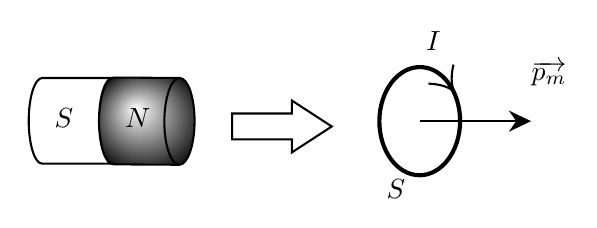
\begin{tikzpicture}[x=0.75pt,y=0.75pt,yscale=-1,xscale=1]
%uncomment if require: \path (0,300); %set diagram left start at 0, and has height of 300

%Shape: Can [id:dp4501980240976837] 
\path  [shading=_jzyajro15,_zfw0x396m] (156.54,117.95) -- (124.97,117.75) .. controls (120.95,117.72) and (117.73,108.34) .. (117.78,96.79) .. controls (117.83,85.24) and (121.13,75.9) .. (125.15,75.93) -- (156.72,76.13) .. controls (160.74,76.16) and (163.96,85.54) .. (163.91,97.09) .. controls (163.86,108.64) and (160.56,117.98) .. (156.54,117.95) .. controls (152.52,117.93) and (149.3,108.54) .. (149.35,96.99) .. controls (149.4,85.45) and (152.7,76.1) .. (156.72,76.13) ; % for fading 
 \draw   (156.54,117.95) -- (124.97,117.75) .. controls (120.95,117.72) and (117.73,108.34) .. (117.78,96.79) .. controls (117.83,85.24) and (121.13,75.9) .. (125.15,75.93) -- (156.72,76.13) .. controls (160.74,76.16) and (163.96,85.54) .. (163.91,97.09) .. controls (163.86,108.64) and (160.56,117.98) .. (156.54,117.95) .. controls (152.52,117.93) and (149.3,108.54) .. (149.35,96.99) .. controls (149.4,85.45) and (152.7,76.1) .. (156.72,76.13) ; % for border 

%Flowchart: Stored Data [id:dp9547962460697509] 
\draw  [fill={rgb, 255:red, 255; green, 255; blue, 255 }  ,fill opacity=1 ] (90.45,76.16) -- (124.31,76.16) .. controls (120.75,76.16) and (117.86,85.39) .. (117.86,96.79) .. controls (117.86,108.18) and (120.75,117.42) .. (124.31,117.42) -- (90.45,117.42) .. controls (86.89,117.42) and (84,108.18) .. (84,96.79) .. controls (84,85.39) and (86.89,76.16) .. (90.45,76.16) -- cycle ;
%Right Arrow [id:dp4508370111610275] 
\draw   (182,93.25) -- (210.8,93.25) -- (210.8,87) -- (230,99.5) -- (210.8,112) -- (210.8,105.75) -- (182,105.75) -- cycle ;
%Shape: Ellipse [id:dp09392556377578465] 
\draw  [line width=1.5]  (272.55,70.88) .. controls (283.29,70.95) and (291.93,82.67) .. (291.84,97.06) .. controls (291.75,111.45) and (282.97,123.06) .. (272.23,123) .. controls (261.49,122.93) and (252.85,111.21) .. (252.94,96.81) .. controls (253.03,82.42) and (261.81,70.81) .. (272.55,70.88) -- cycle ;
\draw   (288.65,69.71) .. controls (287.4,75.03) and (287.5,79.32) .. (288.93,82.6) .. controls (286.16,80.34) and (282.05,79.09) .. (276.6,78.85) ;
%Straight Lines [id:da3699215618726893] 
\draw    (272.39,96.94) -- (323,96.94) ;
\draw [shift={(326,96.94)}, rotate = 180] [fill={rgb, 255:red, 0; green, 0; blue, 0 }  ][line width=0.08]  [draw opacity=0] (10.72,-5.15) -- (0,0) -- (10.72,5.15) -- (7.12,0) -- cycle    ;

% Text Node
\draw (95,89.4) node [anchor=north west][inner sep=0.75pt]    {$S$};
% Text Node
\draw (129,89.4) node [anchor=north west][inner sep=0.75pt]    {$N$};
% Text Node
\draw (274,52.4) node [anchor=north west][inner sep=0.75pt]    {$I$};
% Text Node
\draw (255,123.4) node [anchor=north west][inner sep=0.75pt]    {$S$};
% Text Node
\draw (324.84,66.46) node [anchor=north west][inner sep=0.75pt]    {$\overrightarrow{p_{m}}$};


\end{tikzpicture}
\end{center}
Nam châm hình trụ, cũng như cuộn dây có dòng điện, đặc trưng bởi moment từ $p_{{m}}$. Định nghĩa cho moment từ của vòng mang dòng điện là tích của dòng điện và diện tích của vòng dây.
\[ p_{{m}}=IS.\]
Moment từ như vậy còn được gọi là một lưỡng cực từ. Hình vẽ dưới đây cho ta thấy đường sức từ của một moment từ.
\begin{center}
    \tikzset{every picture/.style={line width=0.75pt}} %set default line width to 0.75pt        

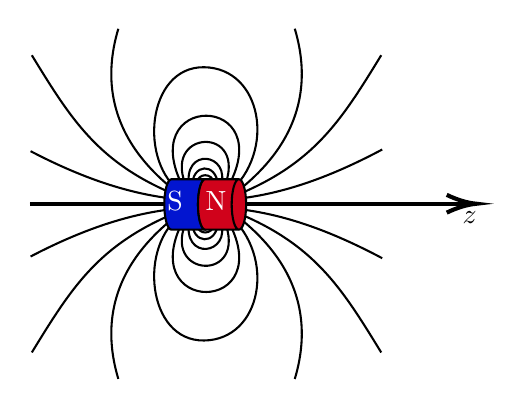
\begin{tikzpicture}[x=0.75pt,y=0.75pt,yscale=-1,xscale=1]
%uncomment if require: \path (0,181); %set diagram left start at 0, and has height of 181

%Straight Lines [id:da06360558422477935] 
\draw [line width=1.5]    (265.97,90.13) -- (478.08,90.13) ;
\draw [shift={(481.08,90.13)}, rotate = 180] [color={rgb, 255:red, 0; green, 0; blue, 0 }  ][line width=1.5]    (14.21,-4.28) .. controls (9.04,-1.82) and (4.3,-0.39) .. (0,0) .. controls (4.3,0.39) and (9.04,1.82) .. (14.21,4.28)   ;
%Curve Lines [id:da6072491279254382] 
\draw    (346.29,80.13) .. controls (347.29,75.13) and (353.63,75.13) .. (354.96,80.13) ;
%Curve Lines [id:da09503964774070672] 
\draw    (344.26,81.6) .. controls (344.1,70.83) and (355.79,69.91) .. (356.7,81.2) ;
%Curve Lines [id:da621421588681335] 
\draw    (342.87,82.68) .. controls (339.02,62.13) and (363.39,65.63) .. (357.91,81.91) ;
%Curve Lines [id:da02158838639918792] 
\draw    (342.07,83.2) .. controls (327.73,53.94) and (372.33,51.74) .. (359.53,82.54) ;
%Curve Lines [id:da4413925308853779] 
\draw    (341.09,84.39) .. controls (313.38,35.24) and (388.81,35.82) .. (360.33,84.14) ;
%Curve Lines [id:da21094694895405253] 
\draw    (339.66,85.24) .. controls (317.99,70.85) and (322.24,23.92) .. (349.99,24.35) .. controls (377.75,24.77) and (384.99,64.85) .. (361.72,85.08) ;
%Curve Lines [id:da10510890003898932] 
\draw    (340.24,87.43) .. controls (331.84,80.23) and (293.84,55.03) .. (308.64,5.83) ;
%Shape: Boxed Bezier Curve [id:dp07893171574002777] 
\draw    (362.05,87.4) .. controls (370.45,80.2) and (408.45,55) .. (393.65,5.8) ;
%Curve Lines [id:da19620814775045292] 
\draw    (266.98,18.6) .. controls (286.58,50.6) and (299.78,71.8) .. (340.24,87.43) ;
%Shape: Boxed Bezier Curve [id:dp04507949087595864] 
\draw    (435.31,18.57) .. controls (415.71,50.57) and (402.51,71.77) .. (362.05,87.4) ;
%Curve Lines [id:da2919180928945344] 
\draw    (266.37,64.8) .. controls (331.38,98.8) and (378.58,94.4) .. (435.78,64) ;
%Straight Lines [id:da33097911884098674] 
\draw    (265.97,90.23) -- (435.78,90.23) ;

%Curve Lines [id:da39653268323313373] 
\draw    (346.29,100.23) .. controls (347.29,105.23) and (353.63,105.23) .. (354.96,100.23) ;
%Curve Lines [id:da0701328024808705] 
\draw    (344.26,98.76) .. controls (344.1,109.53) and (355.79,110.45) .. (356.7,99.17) ;
%Curve Lines [id:da32049824599202115] 
\draw    (342.87,97.69) .. controls (339.02,118.24) and (363.39,114.74) .. (357.91,98.45) ;
%Curve Lines [id:da4693188946066369] 
\draw    (342.07,97.17) .. controls (327.73,126.42) and (372.33,128.62) .. (359.53,97.82) ;
%Curve Lines [id:da9034794333331082] 
\draw    (341.09,95.98) .. controls (313.38,145.12) and (388.81,144.55) .. (360.33,96.22) ;
%Curve Lines [id:da24537082097951046] 
\draw    (339.66,95.12) .. controls (317.99,109.52) and (322.24,156.44) .. (349.99,156.02) .. controls (377.75,155.59) and (384.99,115.52) .. (361.72,95.28) ;
%Curve Lines [id:da5546399747954402] 
\draw    (340.24,92.93) .. controls (331.84,100.13) and (293.84,125.33) .. (308.64,174.53) ;
%Shape: Boxed Bezier Curve [id:dp6444419733416171] 
\draw    (362.05,92.96) .. controls (370.45,100.16) and (408.45,125.36) .. (393.65,174.56) ;
%Curve Lines [id:da6048184278546478] 
\draw    (266.98,161.76) .. controls (286.58,129.76) and (299.78,108.56) .. (340.24,92.93) ;
%Shape: Boxed Bezier Curve [id:dp6696449021155879] 
\draw    (435.31,161.79) .. controls (415.71,129.79) and (402.51,108.59) .. (362.05,92.96) ;
%Curve Lines [id:da5290225403562503] 
\draw    (266.37,115.56) .. controls (331.38,81.57) and (378.58,85.97) .. (435.78,116.37) ;
%Straight Lines [id:da9112047875669156] 
\draw    (265.97,90.13) -- (435.78,90.13) ;

%Shape: Can [id:dp6859889808563859] 
\draw  [fill={rgb, 255:red, 2; green, 21; blue, 208 }  ,fill opacity=1 ] (350.5,102.62) -- (334.26,102.62) .. controls (332.34,102.62) and (330.78,97.18) .. (330.78,90.47) .. controls (330.78,83.76) and (332.34,78.32) .. (334.26,78.32) -- (350.5,78.32) .. controls (352.43,78.32) and (353.98,83.76) .. (353.98,90.47) .. controls (353.98,97.18) and (352.43,102.62) .. (350.5,102.62) .. controls (348.58,102.62) and (347.02,97.18) .. (347.02,90.47) .. controls (347.02,83.76) and (348.58,78.32) .. (350.5,78.32) ;
%Shape: Can [id:dp31443238549542585] 
\draw  [fill={rgb, 255:red, 208; green, 2; blue, 27 }  ,fill opacity=1 ] (366.74,102.62) -- (350.5,102.62) .. controls (348.58,102.62) and (347.02,97.18) .. (347.02,90.47) .. controls (347.02,83.76) and (348.58,78.32) .. (350.5,78.32) -- (366.74,78.32) .. controls (368.67,78.32) and (370.22,83.76) .. (370.22,90.47) .. controls (370.22,97.18) and (368.67,102.62) .. (366.74,102.62) .. controls (364.82,102.62) and (363.26,97.18) .. (363.26,90.47) .. controls (363.26,83.76) and (364.82,78.32) .. (366.74,78.32) ;



% Text Node
\draw (349.22,82.92) node [anchor=north west][inner sep=0.75pt]  [color={rgb, 255:red, 255; green, 255; blue, 255 }  ,opacity=1 ] [align=left] {N};
% Text Node
\draw (330.82,82.75) node [anchor=north west][inner sep=0.75pt]  [color={rgb, 255:red, 255; green, 255; blue, 255 }  ,opacity=1 ] [align=left] {S};
% Text Node
\draw (473,92.4) node [anchor=north west][inner sep=0.75pt]    {$z$};


\end{tikzpicture}
\end{center}
\begin{enumerate}[a)]
    \item Chỉ ra rằng từ trường $B_z$ nằm trên trục đối xứng của vòng được cho bởi biểu thức:
    \[B_{Z}=b \dfrac{p_{m}}{z^{\beta}},\]
    trong đó $z$ là khoảng cách từ một điểm trên trục đối xứng đến tâm của vòng dây. Xác định các tham số $b$ và $\beta$ ở biểu thức trên.
    \item Để cuộn dây có dòng điện (tức là lưỡng cực từ) với moment từ $p_m$ chịu tác dụng của một từ trường đối xứng trục không đồng nhất, cảm ứng từ của nó dọc theo trục $z$ phụ thuộc vào $z$ như hàm $B_{z}(z)$. Trục của lưỡng cực trùng với trục đối xứng của từ trường. 
    \begin{center}
         

\tikzset{every picture/.style={line width=0.75pt}} %set default line width to 0.75pt        

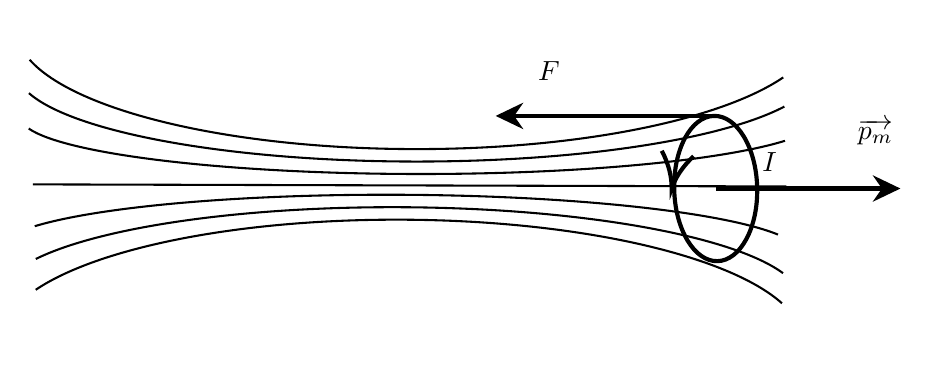
\begin{tikzpicture}[x=0.75pt,y=0.75pt,yscale=-1,xscale=1]
%uncomment if require: \path (0,300); %set diagram left start at 0, and has height of 300

%Shape: Arc [id:dp09724083610265022] 
\draw  [draw opacity=0] (496.56,57.46) .. controls (466.57,77.81) and (398.8,92) .. (320,92) .. controls (230.64,92) and (155.46,73.75) .. (133.49,48.97) -- (320,34) -- cycle ; \draw   (496.56,57.46) .. controls (466.57,77.81) and (398.8,92) .. (320,92) .. controls (230.64,92) and (155.46,73.75) .. (133.49,48.97) ;
%Shape: Arc [id:dp9573942278688676] 
\draw  [draw opacity=0] (497.09,71.52) .. controls (467.39,87.1) and (399.28,98) .. (320,98) .. controls (230.13,98) and (154.6,84) .. (133.12,65.04) -- (320,54) -- cycle ; \draw   (497.09,71.52) .. controls (467.39,87.1) and (399.28,98) .. (320,98) .. controls (230.13,98) and (154.6,84) .. (133.12,65.04) ;
%Shape: Arc [id:dp5398400734661393] 
\draw  [draw opacity=0] (497.38,88) .. controls (466.83,97.44) and (399.79,104) .. (322,104) .. controls (228.9,104) and (151.19,94.61) .. (133.02,82.11) -- (322,76.5) -- cycle ; \draw   (497.38,88) .. controls (466.83,97.44) and (399.79,104) .. (322,104) .. controls (228.9,104) and (151.19,94.61) .. (133.02,82.11) ;
%Shape: Arc [id:dp5931355655659283] 
\draw  [draw opacity=0] (136.4,159.79) .. controls (166.42,139.54) and (234.33,125.63) .. (313.23,126.01) .. controls (398.2,126.41) and (470.27,143.25) .. (495.93,166.29) -- (312.96,184) -- cycle ; \draw   (136.4,159.79) .. controls (166.42,139.54) and (234.33,125.63) .. (313.23,126.01) .. controls (398.2,126.41) and (470.27,143.25) .. (495.93,166.29) ;
%Shape: Arc [id:dp18584702804365694] 
\draw  [draw opacity=0] (136.42,144.95) .. controls (166.88,129.89) and (234.18,119.63) .. (312.26,120) .. controls (398.87,120.41) and (472.09,133.76) .. (496.44,151.79) -- (312.05,164) -- cycle ; \draw   (136.42,144.95) .. controls (166.88,129.89) and (234.18,119.63) .. (312.26,120) .. controls (398.87,120.41) and (472.09,133.76) .. (496.44,151.79) ;
%Shape: Arc [id:dp843366810007487] 
\draw  [draw opacity=0] (135.94,129.15) .. controls (166.63,119.86) and (233.81,113.63) .. (311.71,114) .. controls (395.9,114.39) and (467.49,122.38) .. (494.01,133.18) -- (311.58,141.5) -- cycle ; \draw   (135.94,129.15) .. controls (166.63,119.86) and (233.81,113.63) .. (311.71,114) .. controls (395.9,114.39) and (467.49,122.38) .. (494.01,133.18) ;
%Straight Lines [id:da0825312466176309] 
\draw    (498,110) -- (135,109) ;
%Shape: Ellipse [id:dp154624595511056] 
\draw  [line width=1.5]  (463.14,76.01) .. controls (474.19,75.74) and (483.52,91.19) .. (483.99,110.51) .. controls (484.47,129.84) and (475.9,145.72) .. (464.86,145.99) .. controls (453.81,146.26) and (444.48,130.81) .. (444.01,111.49) .. controls (443.53,92.16) and (452.1,76.28) .. (463.14,76.01) -- cycle ;
\draw  [line width=1.5]  (453.33,95.42) .. controls (448.11,100.37) and (444.6,105.61) .. (442.77,111.14) .. controls (442.89,105.32) and (441.32,99.21) .. (438.04,92.8) ;
%Straight Lines [id:da9522131982799203] 
\draw [line width=1.5]    (464,111) -- (549,111) ;
\draw [shift={(553,111)}, rotate = 180] [fill={rgb, 255:red, 0; green, 0; blue, 0 }  ][line width=0.08]  [draw opacity=0] (13.4,-6.43) -- (0,0) -- (13.4,6.44) -- (8.9,0) -- cycle    ;
%Straight Lines [id:da050548300708038396] 
\draw [line width=1.5]    (463.14,76.01) -- (362,76.01) ;
\draw [shift={(358,76.01)}, rotate = 360] [fill={rgb, 255:red, 0; green, 0; blue, 0 }  ][line width=0.08]  [draw opacity=0] (13.4,-6.43) -- (0,0) -- (13.4,6.44) -- (8.9,0) -- cycle    ;

% Text Node
\draw (531,76.4) node [anchor=north west][inner sep=0.75pt]    {$\overrightarrow{p_{m}}$};
% Text Node
\draw (377,48.4) node [anchor=north west][inner sep=0.75pt]    {$\ot{F}$};
% Text Node
\draw (485,92.4) node [anchor=north west][inner sep=0.75pt]    {$I$};


\end{tikzpicture}
    \end{center}
    Chứng tỏ rằng lực do từ trường tác dụng lên lưỡng cực cho bởi:
    \[F_{z}=-p_{m} \dfrac{\dd B_{z}}{\dd z}.\]
\end{enumerate}
\item \textbf{Dao động của nam châm.}\\
Nam châm hình trụ khối lượng $m$ và moment từ $p_m$, được gắn vào lò xo có độ cứng $k$ sao cho nó có thể dao động dọc theo trục nằm ngang hướng dọc theo moment từ.
\begin{enumerate}[a)]
    \item Tìm tần số dao động tự do $\omega_0$ của nam châm trong điều kiện không có trường lực bên ngoài.
    \item Tại một khoảng cách $z$ so với vị trí cân bằng của nam châm, người ta đặt một đĩa kim loại nhỏ sao cho trục của nó trùng với trục của nam châm. Đĩa có bán kính $R$ và bề dày $h~(h \ll R \ll z)$, điện trở suất của vật liệu làm đĩa là $\rho$, và độ từ thẩm đặt bằng $\mu=1$. Nam châm được đưa ra khỏi vị trí cân bằng và bắt đầu thực hiện dao động nhỏ. Dao động được mô tả bởi hàm $x(t)$, trong đó $x \ll z$.\\
    Tìm lực $F(x, v)$ do đĩa tác dụng lên nam châm dưới dạng hàm của tọa độ $x$ và vận tốc $v$ của nó. Viết phương trình chuyển động của nam châm.
\begin{center}
% Pattern Info
 
\tikzset{
pattern size/.store in=\mcSize, 
pattern size = 5pt,
pattern thickness/.store in=\mcThickness, 
pattern thickness = 0.3pt,
pattern radius/.store in=\mcRadius, 
pattern radius = 1pt}
\makeatletter
\pgfutil@ifundefined{pgf@pattern@_chcrj0tny}{
\pgfdeclarepatternformonly[\mcThickness,\mcSize]{_chcrj0tny}
{\pgfpointorigin}
{\pgfpoint{\mcSize+\mcThickness}{\mcSize+\mcThickness}}
{\pgfpoint{\mcSize}{\mcSize}}{
\pgfsetcolor{\tikz@pattern@color}
\pgfsetlinewidth{\mcThickness}
\pgfpathmoveto{\pgfpointorigin}
\pgfpathlineto{\pgfpoint{0pt}{0.5*\mcSize}}
\pgfpathlineto{\pgfpoint{\mcSize}{0.5*\mcSize}}
\pgfpathmoveto{\pgfpoint{0.5*\mcSize}{0.5*\mcSize}}
\pgfpathlineto{\pgfpoint{0.5*\mcSize}{\mcSize}}
\pgfpathmoveto{\pgfpoint{0pt}{\mcSize}}
\pgfpathlineto{\pgfpoint{\mcSize}{\mcSize}}
\pgfusepath{stroke}}}
\makeatother

% Gradient Info
  
\tikzset {_gge74cn1a/.code = {\pgfsetadditionalshadetransform{ \pgftransformshift{\pgfpoint{0 bp } { 0 bp }  }  \pgftransformrotate{0 }  \pgftransformscale{2 }  }}}
\pgfdeclarehorizontalshading{_mcpwhh0at}{150bp}{rgb(0bp)=(1,1,1);
rgb(37.5bp)=(1,1,1);
rgb(50bp)=(0.95,0.95,0.95);
rgb(50.25bp)=(0.88,0.88,0.88);
rgb(62.5bp)=(0.96,0.96,0.96);
rgb(100bp)=(0.96,0.96,0.96)}

% Gradient Info
  
\tikzset {_00lsj81k4/.code = {\pgfsetadditionalshadetransform{ \pgftransformshift{\pgfpoint{89.1 bp } { -108.9 bp }  }  \pgftransformscale{1.32 }  }}}
\pgfdeclareradialshading{_oq1z91hja}{\pgfpoint{-72bp}{88bp}}{rgb(0bp)=(1,1,1);
rgb(0bp)=(1,1,1);
rgb(25bp)=(0,0,0);
rgb(400bp)=(0,0,0)}

% Gradient Info
  
\tikzset {_82em7jkyg/.code = {\pgfsetadditionalshadetransform{ \pgftransformshift{\pgfpoint{0 bp } { 0 bp }  }  \pgftransformrotate{0 }  \pgftransformscale{2 }  }}}
\pgfdeclarehorizontalshading{_iwlvlrkw7}{150bp}{rgb(0bp)=(0.96,0.96,0.96);
rgb(37.5bp)=(0.96,0.96,0.96);
rgb(42.75bp)=(0.86,0.86,0.89);
rgb(49.75bp)=(0.72,0.73,0.78);
rgb(57.5bp)=(0.87,0.87,0.89);
rgb(62.5bp)=(0.96,0.96,0.96);
rgb(100bp)=(0.96,0.96,0.96)}
\tikzset{every picture/.style={line width=0.75pt}} %set default line width to 0.75pt        

\begin{tikzpicture}[x=0.75pt,y=0.75pt,yscale=-0.7,xscale=0.7]
%uncomment if require: \path (0,300); %set diagram left start at 0, and has height of 300

%Shape: Rectangle [id:dp26559850878070734] 
\draw  [pattern=_chcrj0tny,pattern size=6pt,pattern thickness=0.75pt,pattern radius=0pt, pattern color={rgb, 255:red, 0; green, 0; blue, 0}] (35,191) -- (35,130) -- (48,130) -- (48,191) -- cycle ;
%Shape: Spring [id:dp37505721031698325] 
\draw   (48.96,153.67) .. controls (49.35,148.18) and (51.61,142.7) .. (56.11,142.71) .. controls (65.11,142.74) and (65.06,164.68) .. (59.06,164.67) .. controls (53.06,164.65) and (53.11,142.7) .. (62.11,142.73) .. controls (71.11,142.75) and (71.06,164.7) .. (65.06,164.68) .. controls (59.06,164.67) and (59.11,142.72) .. (68.11,142.74) .. controls (77.11,142.77) and (77.06,164.71) .. (71.06,164.7) .. controls (65.06,164.68) and (65.11,142.74) .. (74.11,142.76) .. controls (83.11,142.78) and (83.06,164.73) .. (77.06,164.71) .. controls (71.06,164.7) and (71.11,142.75) .. (80.11,142.78) .. controls (89.11,142.8) and (89.05,164.75) .. (83.06,164.73) .. controls (77.06,164.71) and (77.11,142.77) .. (86.11,142.79) .. controls (95.11,142.81) and (95.05,164.76) .. (89.05,164.75) .. controls (83.06,164.73) and (83.11,142.78) .. (92.11,142.81) .. controls (101.11,142.83) and (101.05,164.78) .. (95.05,164.76) .. controls (89.05,164.75) and (89.11,142.8) .. (98.11,142.82) .. controls (107.11,142.85) and (107.05,164.79) .. (101.05,164.78) .. controls (95.05,164.76) and (95.11,142.81) .. (104.11,142.84) .. controls (113.11,142.86) and (113.05,164.81) .. (107.05,164.79) .. controls (101.05,164.78) and (101.11,142.83) .. (110.11,142.85) .. controls (119.11,142.88) and (119.05,164.82) .. (113.05,164.81) .. controls (107.05,164.79) and (107.11,142.85) .. (116.11,142.87) .. controls (125.11,142.89) and (125.05,164.84) .. (119.05,164.82) .. controls (113.05,164.81) and (113.11,142.86) .. (122.11,142.89) .. controls (131.11,142.91) and (131.05,164.86) .. (125.05,164.84) .. controls (119.05,164.82) and (119.11,142.88) .. (128.11,142.9) .. controls (137.11,142.92) and (137.05,164.87) .. (131.05,164.86) .. controls (125.05,164.84) and (125.11,142.89) .. (134.11,142.92) .. controls (143.11,142.94) and (143.05,164.89) .. (137.05,164.87) .. controls (131.05,164.86) and (131.11,142.91) .. (140.11,142.93) .. controls (149.11,142.96) and (149.05,164.9) .. (143.05,164.89) .. controls (137.05,164.87) and (137.11,142.92) .. (146.11,142.95) .. controls (155.11,142.97) and (155.05,164.92) .. (149.05,164.9) .. controls (143.05,164.89) and (143.11,142.94) .. (152.11,142.96) .. controls (161.11,142.99) and (161.05,164.93) .. (155.05,164.92) .. controls (149.05,164.9) and (149.11,142.96) .. (158.11,142.98) .. controls (167.11,143) and (167.05,164.95) .. (161.05,164.93) .. controls (155.05,164.92) and (155.11,142.97) .. (164.11,143) .. controls (173.11,143.02) and (173.05,164.97) .. (167.05,164.95) .. controls (161.05,164.93) and (161.11,142.99) .. (170.11,143.01) .. controls (179.11,143.03) and (179.05,164.98) .. (173.05,164.97) .. controls (167.05,164.95) and (167.11,143) .. (176.11,143.03) .. controls (185.11,143.05) and (185.05,165) .. (179.05,164.98) .. controls (173.05,164.97) and (173.11,143.02) .. (182.11,143.04) .. controls (183.7,143.05) and (185.01,143.74) .. (186.05,144.87) ;
%Flowchart: Stored Data [id:dp8176790316288902] 
\path  [shading=_mcpwhh0at,_gge74cn1a] (189.04,134) -- (205,134) .. controls (203.32,134) and (201.96,142.95) .. (201.96,154) .. controls (201.96,165.05) and (203.32,174) .. (205,174) -- (189.04,174) .. controls (187.36,174) and (186,165.05) .. (186,154) .. controls (186,142.95) and (187.36,134) .. (189.04,134) -- cycle ; % for fading 
 \draw   (189.04,134) -- (205,134) .. controls (203.32,134) and (201.96,142.95) .. (201.96,154) .. controls (201.96,165.05) and (203.32,174) .. (205,174) -- (189.04,174) .. controls (187.36,174) and (186,165.05) .. (186,154) .. controls (186,142.95) and (187.36,134) .. (189.04,134) -- cycle ; % for border 

%Flowchart: Direct Access Storage [id:dp5399580700082982] 
\path  [shading=_oq1z91hja,_00lsj81k4] (219.32,174) -- (205.64,174) .. controls (203.61,174) and (201.96,165.05) .. (201.96,154) .. controls (201.96,142.95) and (203.61,134) .. (205.64,134) -- (219.32,134)(223,154) .. controls (223,165.05) and (221.35,174) .. (219.32,174) .. controls (217.28,174) and (215.64,165.05) .. (215.64,154) .. controls (215.64,142.95) and (217.28,134) .. (219.32,134) .. controls (221.35,134) and (223,142.95) .. (223,154) ; % for fading 
 \draw   (219.32,174) -- (205.64,174) .. controls (203.61,174) and (201.96,165.05) .. (201.96,154) .. controls (201.96,142.95) and (203.61,134) .. (205.64,134) -- (219.32,134)(223,154) .. controls (223,165.05) and (221.35,174) .. (219.32,174) .. controls (217.28,174) and (215.64,165.05) .. (215.64,154) .. controls (215.64,142.95) and (217.28,134) .. (219.32,134) .. controls (221.35,134) and (223,142.95) .. (223,154) ; % for border 

%Straight Lines [id:da9167583407483029] 
\draw [line width=1.5]    (215.64,154) -- (253,154) ;
\draw [shift={(257,154)}, rotate = 180] [fill={rgb, 255:red, 0; green, 0; blue, 0 }  ][line width=0.08]  [draw opacity=0] (15.6,-3.9) -- (0,0) -- (15.6,3.9) -- cycle    ;
%Straight Lines [id:da47575998082208115] 
\draw    (62,192) -- (390,192) ;
\draw [shift={(393,192)}, rotate = 180] [fill={rgb, 255:red, 0; green, 0; blue, 0 }  ][line width=0.08]  [draw opacity=0] (10.72,-5.15) -- (0,0) -- (10.72,5.15) -- (7.12,0) -- cycle    ;
%Straight Lines [id:da319713090471194] 
\draw    (203,183) -- (203,200) ;

%Straight Lines [id:da1365287208408681] 
\draw [line width=1.5]    (169,200) -- (237,200) ;
\draw [shift={(241,200)}, rotate = 180] [fill={rgb, 255:red, 0; green, 0; blue, 0 }  ][line width=0.08]  [draw opacity=0] (13.4,-6.43) -- (0,0) -- (13.4,6.44) -- (8.9,0) -- cycle    ;
\draw [shift={(165,200)}, rotate = 0] [fill={rgb, 255:red, 0; green, 0; blue, 0 }  ][line width=0.08]  [draw opacity=0] (13.4,-6.43) -- (0,0) -- (13.4,6.44) -- (8.9,0) -- cycle    ;
%Straight Lines [id:da842491381532174] 
\draw  [dash pattern={on 4.5pt off 4.5pt}]  (257,154) -- (523,154) ;
%Flowchart: Direct Access Storage [id:dp9916978957980093] 
\path  [shading=_iwlvlrkw7,_82em7jkyg] (548.58,205) -- (528.43,205) .. controls (525.43,205) and (523,182.17) .. (523,154) .. controls (523,125.83) and (525.43,103) .. (528.43,103) -- (548.58,103)(554,154) .. controls (554,182.17) and (551.57,205) .. (548.58,205) .. controls (545.58,205) and (543.15,182.17) .. (543.15,154) .. controls (543.15,125.83) and (545.58,103) .. (548.58,103) .. controls (551.57,103) and (554,125.83) .. (554,154) ; % for fading 
 \draw   (548.58,205) -- (528.43,205) .. controls (525.43,205) and (523,182.17) .. (523,154) .. controls (523,125.83) and (525.43,103) .. (528.43,103) -- (548.58,103)(554,154) .. controls (554,182.17) and (551.57,205) .. (548.58,205) .. controls (545.58,205) and (543.15,182.17) .. (543.15,154) .. controls (543.15,125.83) and (545.58,103) .. (548.58,103) .. controls (551.57,103) and (554,125.83) .. (554,154) ; % for border 

%Straight Lines [id:da3012981700387881] 
\draw    (205,115) -- (523,115) ;
\draw [shift={(526,115)}, rotate = 180] [fill={rgb, 255:red, 0; green, 0; blue, 0 }  ][line width=0.08]  [draw opacity=0] (10.72,-5.15) -- (0,0) -- (10.72,5.15) -- (7.12,0) -- cycle    ;
\draw [shift={(202,115)}, rotate = 0] [fill={rgb, 255:red, 0; green, 0; blue, 0 }  ][line width=0.08]  [draw opacity=0] (10.72,-5.15) -- (0,0) -- (10.72,5.15) -- (7.12,0) -- cycle    ;
%Straight Lines [id:da43849354039646804] 
\draw    (490.43,103) -- (525.43,103) ;
\draw [shift={(528.43,103)}, rotate = 180] [fill={rgb, 255:red, 0; green, 0; blue, 0 }  ][line width=0.08]  [draw opacity=0] (10.72,-5.15) -- (0,0) -- (10.72,5.15) -- (7.12,0) -- cycle    ;
%Straight Lines [id:da20735474908532348] 
\draw    (587.58,103) -- (551.58,103) ;
\draw [shift={(548.58,103)}, rotate = 360] [fill={rgb, 255:red, 0; green, 0; blue, 0 }  ][line width=0.08]  [draw opacity=0] (10.72,-5.15) -- (0,0) -- (10.72,5.15) -- (7.12,0) -- cycle    ;
%Straight Lines [id:da8489570030372383] 
\draw    (548,150) -- (548.55,203) ;
\draw [shift={(548.58,205)}, rotate = 269.4] [color={rgb, 255:red, 0; green, 0; blue, 0 }  ][line width=0.75]    (10.93,-3.29) .. controls (6.95,-1.4) and (3.31,-0.3) .. (0,0) .. controls (3.31,0.3) and (6.95,1.4) .. (10.93,3.29)   ;

% Text Node
\draw (227,119.4) node [anchor=north west][inner sep=0.75pt]    {$\overrightarrow{p_{m}}$};
% Text Node
\draw (182,116.4) node [anchor=north west][inner sep=0.75pt]    {$m$};
% Text Node
\draw (378,198.4) node [anchor=north west][inner sep=0.75pt]    {$x$};
% Text Node
\draw (199,200.4) node [anchor=north west][inner sep=0.75pt]    {$\omega_{0}$};
% Text Node
\draw (365,93.4) node [anchor=north west][inner sep=0.75pt]    {$z$};
% Text Node
\draw (535,82.4) node [anchor=north west][inner sep=0.75pt]    {$h$};
% Text Node
\draw (556,165.4) node [anchor=north west][inner sep=0.75pt]    {$R$};
\end{tikzpicture}
 \end{center}
 
\item Tìm sự thay đổi tương đối $\dfrac{\Delta \omega}{\omega_0}$ của tần số dao động của nam châm do ảnh hưởng của đĩa gây ra.
\item Giả sử rằng độ suy giảm là khá yếu, hãy tính thời gian suy giảm đặc trưng dao động của quả cầu.
\item Chứng tỏ rằng phần cơ năng mất đi của nam châm bằng nhiệt lượng toả ra ở đĩa trong cùng một khoảng thời gian.
\end{enumerate}
\begin{center}
    \textbf{Một số gợi ý toán học:}\\
    \end{center}
    Phương trình vi phân có dạng:
    \[
\dfrac{\dd^{2} x}{\dd t^{2}}+2 \dfrac{\beta \dd x}{\dd t}+\omega_{0}^{2} x=0.
\]
Cho ta nghiệm:
\[
x(t)=A \exp \left(-\dfrac{t}{\tau}\right) \cos (\omega t+\varphi),
\]
trong đó $\omega=\sqrt{\omega_{0}^{2}-\beta^{2}}$ là tần số dao động tắt dần, $\dfrac{1}{\beta}$ là hệ số suy giảm và các tham số $A$, $\varphi$ có thể xác định được từ điều kiện ban đầu.\\
\textbf{Lưu ý:} Khi $x \ll 1$, ta có thể dùng công thức xấp xỉ sau:
\[(1+x)^{\alpha} \approx 1+\alpha x.\]
\end{enumerate}
\begin{center}
\textbf{Phần II: Điện tích}
\end{center}
\begin{enumerate}[1)]
\item \textbf{Giới thiệu lí thuyết:} \\
Một hệ gồm hai điện tích cùng độ lớn nhưng trái dấu $(-q,+q)$ đặt cách nhau một khoảng cách cố định $l$ được gọi là một lưỡng cực điện. Lưỡng cực điện được đặc trưng bởi moment lưỡng cực điện:
\[p_e=ql.\]
\begin{center}
    

% Gradient Info
  
\tikzset {_pog7kp549/.code = {\pgfsetadditionalshadetransform{ \pgftransformshift{\pgfpoint{89.1 bp } { -128.7 bp }  }  \pgftransformscale{1.32 }  }}}
\pgfdeclareradialshading{_89qvhd3qs}{\pgfpoint{-72bp}{104bp}}{rgb(0bp)=(1,1,1);
rgb(0bp)=(1,1,1);
rgb(25bp)=(0.48,0.15,0.15);
rgb(400bp)=(0.48,0.15,0.15)}

% Gradient Info
  
\tikzset {_bbmamr3ya/.code = {\pgfsetadditionalshadetransform{ \pgftransformshift{\pgfpoint{89.1 bp } { -128.7 bp }  }  \pgftransformscale{1.32 }  }}}
\pgfdeclareradialshading{_x568on63t}{\pgfpoint{-72bp}{104bp}}{rgb(0bp)=(1,1,1);
rgb(0bp)=(1,1,1);
rgb(25bp)=(0.48,0.15,0.15);
rgb(400bp)=(0.48,0.15,0.15)}
\tikzset{every picture/.style={line width=0.75pt}} %set default line width to 0.75pt        

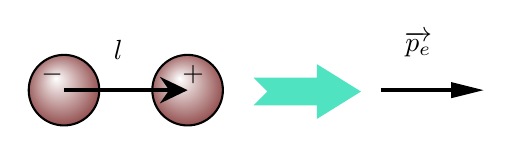
\begin{tikzpicture}[x=0.75pt,y=0.75pt,yscale=-1,xscale=1]
%uncomment if require: \path (0,300); %set diagram left start at 0, and has height of 300

%Shape: Circle [id:dp5808415922296699] 
\path  [shading=_89qvhd3qs,_pog7kp549] (126.45,98) .. controls (126.45,88.61) and (134.06,81) .. (143.45,81) .. controls (152.83,81) and (160.45,88.61) .. (160.45,98) .. controls (160.45,107.39) and (152.83,115) .. (143.45,115) .. controls (134.06,115) and (126.45,107.39) .. (126.45,98) -- cycle ; % for fading 
 \draw   (126.45,98) .. controls (126.45,88.61) and (134.06,81) .. (143.45,81) .. controls (152.83,81) and (160.45,88.61) .. (160.45,98) .. controls (160.45,107.39) and (152.83,115) .. (143.45,115) .. controls (134.06,115) and (126.45,107.39) .. (126.45,98) -- cycle ; % for border 

%Shape: Circle [id:dp1594954734323084] 
\path  [shading=_x568on63t,_bbmamr3ya] (186,98) .. controls (186,88.61) and (193.61,81) .. (203,81) .. controls (212.39,81) and (220,88.61) .. (220,98) .. controls (220,107.39) and (212.39,115) .. (203,115) .. controls (193.61,115) and (186,107.39) .. (186,98) -- cycle ; % for fading 
 \draw   (186,98) .. controls (186,88.61) and (193.61,81) .. (203,81) .. controls (212.39,81) and (220,88.61) .. (220,98) .. controls (220,107.39) and (212.39,115) .. (203,115) .. controls (193.61,115) and (186,107.39) .. (186,98) -- cycle ; % for border 

%Straight Lines [id:da4684152726117038] 
\draw [line width=1.5]    (143.45,98) -- (199,98) ;
\draw [shift={(203,98)}, rotate = 180] [fill={rgb, 255:red, 0; green, 0; blue, 0 }  ][line width=0.08]  [draw opacity=0] (13.4,-6.43) -- (0,0) -- (13.4,6.44) -- (8.9,0) -- cycle    ;
%Notched Right Arrow [id:dp5971022441085105] 
\draw  [color={rgb, 255:red, 80; green, 227; blue, 194 }  ,draw opacity=1 ][fill={rgb, 255:red, 80; green, 227; blue, 194 }  ,fill opacity=1 ] (236,92.51) -- (265.76,92.51) -- (265.76,86.34) -- (285.59,98.67) -- (265.76,111) -- (265.76,104.84) -- (236,104.84) -- (242.16,98.67) -- cycle ;
%Straight Lines [id:da9075858395075501] 
\draw [line width=1.5]    (296,98) -- (341.59,98) ;
\draw [shift={(345.59,98)}, rotate = 180] [fill={rgb, 255:red, 0; green, 0; blue, 0 }  ][line width=0.08]  [draw opacity=0] (15.6,-3.9) -- (0,0) -- (15.6,3.9) -- cycle    ;

% Text Node
\draw (199,84.4) node [anchor=north west][inner sep=0.75pt]    {$+$};
% Text Node
\draw (131,84.4) node [anchor=north west][inner sep=0.75pt]    {$-$};
% Text Node
\draw (166,72.4) node [anchor=north west][inner sep=0.75pt]    {$\ot{l}$};
% Text Node
\draw (306,68.4) node [anchor=north west][inner sep=0.75pt]    {$\overrightarrow{p_{e}}$};
\end{tikzpicture}
\end{center}
\begin{enumerate}[a)]
\item Điện trường gây ra bởi lưỡng cực điện tại khoảng cách $z \gg l$ ngay trên trục của nó được cho bởi biểu thức:
\[
E=a \dfrac{p_{e}}{z^{\alpha}}.
\]
Xác định $a, \alpha$ trong biểu thức trên.
\end{enumerate}
\item 
\textbf{Dao động của quả cầu tích điện.}\\
Một quả cầu nhỏ khối lượng $m$ mang điện tích $q$ được gắn vào một lò xo không dẫn điện có độ cứng $k$ và có thể dao động điều hòa dọc theo trục hoành $x$. Tại một khoảng cách $z$ nào đó so với vị trí cân bằng của quả cầu, một đĩa nhỏ bằng kim loại dẫn điện hoàn toàn được cố định sao cho trục của nó trùng với trục $x$. Đĩa có bán kính $R$ và bề dày $h (h\ll R\ll  z)$.
\begin{center}
    

% Pattern Info
 
\tikzset{
pattern size/.store in=\mcSize, 
pattern size = 5pt,
pattern thickness/.store in=\mcThickness, 
pattern thickness = 0.3pt,
pattern radius/.store in=\mcRadius, 
pattern radius = 1pt}
\makeatletter
\pgfutil@ifundefined{pgf@pattern@_28fkg6inr}{
\pgfdeclarepatternformonly[\mcThickness,\mcSize]{_28fkg6inr}
{\pgfpointorigin}
{\pgfpoint{\mcSize+\mcThickness}{\mcSize+\mcThickness}}
{\pgfpoint{\mcSize}{\mcSize}}{
\pgfsetcolor{\tikz@pattern@color}
\pgfsetlinewidth{\mcThickness}
\pgfpathmoveto{\pgfpointorigin}
\pgfpathlineto{\pgfpoint{0pt}{0.5*\mcSize}}
\pgfpathlineto{\pgfpoint{\mcSize}{0.5*\mcSize}}
\pgfpathmoveto{\pgfpoint{0.5*\mcSize}{0.5*\mcSize}}
\pgfpathlineto{\pgfpoint{0.5*\mcSize}{\mcSize}}
\pgfpathmoveto{\pgfpoint{0pt}{\mcSize}}
\pgfpathlineto{\pgfpoint{\mcSize}{\mcSize}}
\pgfusepath{stroke}}}
\makeatother

% Gradient Info
  
\tikzset {_e6ep1179j/.code = {\pgfsetadditionalshadetransform{ \pgftransformshift{\pgfpoint{0 bp } { 0 bp }  }  \pgftransformrotate{0 }  \pgftransformscale{2 }  }}}
\pgfdeclarehorizontalshading{_muca7sf3u}{150bp}{rgb(0bp)=(0.96,0.96,0.96);
rgb(37.5bp)=(0.96,0.96,0.96);
rgb(42.75bp)=(0.86,0.86,0.89);
rgb(49.75bp)=(0.72,0.73,0.78);
rgb(57.5bp)=(0.87,0.87,0.89);
rgb(62.5bp)=(0.96,0.96,0.96);
rgb(100bp)=(0.96,0.96,0.96)}

% Gradient Info
  
\tikzset {_6o6a19847/.code = {\pgfsetadditionalshadetransform{ \pgftransformshift{\pgfpoint{89.1 bp } { -108.9 bp }  }  \pgftransformscale{1.32 }  }}}
\pgfdeclareradialshading{_a6rm7mgci}{\pgfpoint{-72bp}{88bp}}{rgb(0bp)=(1,1,1);
rgb(0bp)=(1,1,1);
rgb(25bp)=(0,0,0);
rgb(400bp)=(0,0,0)}
\tikzset{every picture/.style={line width=0.75pt}} %set default line width to 0.75pt        

\begin{tikzpicture}[x=0.75pt,y=0.75pt,yscale=-0.7,xscale=0.7]
%uncomment if require: \path (0,300); %set diagram left start at 0, and has height of 300

%Shape: Rectangle [id:dp26559850878070734] 
\draw  [pattern=_28fkg6inr,pattern size=6pt,pattern thickness=0.75pt,pattern radius=0pt, pattern color={rgb, 255:red, 0; green, 0; blue, 0}] (35,191) -- (35,130) -- (48,130) -- (48,191) -- cycle ;
%Shape: Spring [id:dp37505721031698325] 
\draw   (48.96,153.67) .. controls (49.35,148.18) and (51.61,142.7) .. (56.11,142.71) .. controls (65.11,142.74) and (65.06,164.68) .. (59.06,164.67) .. controls (53.06,164.65) and (53.11,142.7) .. (62.11,142.73) .. controls (71.11,142.75) and (71.06,164.7) .. (65.06,164.68) .. controls (59.06,164.67) and (59.11,142.72) .. (68.11,142.74) .. controls (77.11,142.77) and (77.06,164.71) .. (71.06,164.7) .. controls (65.06,164.68) and (65.11,142.74) .. (74.11,142.76) .. controls (83.11,142.78) and (83.06,164.73) .. (77.06,164.71) .. controls (71.06,164.7) and (71.11,142.75) .. (80.11,142.78) .. controls (89.11,142.8) and (89.05,164.75) .. (83.06,164.73) .. controls (77.06,164.71) and (77.11,142.77) .. (86.11,142.79) .. controls (95.11,142.81) and (95.05,164.76) .. (89.05,164.75) .. controls (83.06,164.73) and (83.11,142.78) .. (92.11,142.81) .. controls (101.11,142.83) and (101.05,164.78) .. (95.05,164.76) .. controls (89.05,164.75) and (89.11,142.8) .. (98.11,142.82) .. controls (107.11,142.85) and (107.05,164.79) .. (101.05,164.78) .. controls (95.05,164.76) and (95.11,142.81) .. (104.11,142.84) .. controls (113.11,142.86) and (113.05,164.81) .. (107.05,164.79) .. controls (101.05,164.78) and (101.11,142.83) .. (110.11,142.85) .. controls (119.11,142.88) and (119.05,164.82) .. (113.05,164.81) .. controls (107.05,164.79) and (107.11,142.85) .. (116.11,142.87) .. controls (125.11,142.89) and (125.05,164.84) .. (119.05,164.82) .. controls (113.05,164.81) and (113.11,142.86) .. (122.11,142.89) .. controls (131.11,142.91) and (131.05,164.86) .. (125.05,164.84) .. controls (119.05,164.82) and (119.11,142.88) .. (128.11,142.9) .. controls (137.11,142.92) and (137.05,164.87) .. (131.05,164.86) .. controls (125.05,164.84) and (125.11,142.89) .. (134.11,142.92) .. controls (143.11,142.94) and (143.05,164.89) .. (137.05,164.87) .. controls (131.05,164.86) and (131.11,142.91) .. (140.11,142.93) .. controls (149.11,142.96) and (149.05,164.9) .. (143.05,164.89) .. controls (137.05,164.87) and (137.11,142.92) .. (146.11,142.95) .. controls (155.11,142.97) and (155.05,164.92) .. (149.05,164.9) .. controls (143.05,164.89) and (143.11,142.94) .. (152.11,142.96) .. controls (161.11,142.99) and (161.05,164.93) .. (155.05,164.92) .. controls (149.05,164.9) and (149.11,142.96) .. (158.11,142.98) .. controls (167.11,143) and (167.05,164.95) .. (161.05,164.93) .. controls (155.05,164.92) and (155.11,142.97) .. (164.11,143) .. controls (173.11,143.02) and (173.05,164.97) .. (167.05,164.95) .. controls (161.05,164.93) and (161.11,142.99) .. (170.11,143.01) .. controls (179.11,143.03) and (179.05,164.98) .. (173.05,164.97) .. controls (167.05,164.95) and (167.11,143) .. (176.11,143.03) .. controls (185.11,143.05) and (185.05,165) .. (179.05,164.98) .. controls (173.05,164.97) and (173.11,143.02) .. (182.11,143.04) .. controls (183.7,143.05) and (185.01,143.74) .. (186.05,144.87) ;
%Straight Lines [id:da5598052361157017] 
\draw    (211.32,154) -- (428.32,154) ;
\draw [shift={(431.32,154)}, rotate = 180] [fill={rgb, 255:red, 0; green, 0; blue, 0 }  ][line width=0.08]  [draw opacity=0] (10.72,-5.15) -- (0,0) -- (10.72,5.15) -- (7.12,0) -- cycle    ;
%Straight Lines [id:da1365287208408681] 
\draw [line width=1.5]    (169,200) -- (237,200) ;
\draw [shift={(241,200)}, rotate = 180] [fill={rgb, 255:red, 0; green, 0; blue, 0 }  ][line width=0.08]  [draw opacity=0] (13.4,-6.43) -- (0,0) -- (13.4,6.44) -- (8.9,0) -- cycle    ;
\draw [shift={(165,200)}, rotate = 0] [fill={rgb, 255:red, 0; green, 0; blue, 0 }  ][line width=0.08]  [draw opacity=0] (13.4,-6.43) -- (0,0) -- (13.4,6.44) -- (8.9,0) -- cycle    ;
%Straight Lines [id:da842491381532174] 
\draw  [dash pattern={on 4.5pt off 4.5pt}]  (247.5,154) -- (523,154) ;
%Flowchart: Direct Access Storage [id:dp9916978957980093] 
\path  [shading=_muca7sf3u,_e6ep1179j] (548.58,205) -- (528.43,205) .. controls (525.43,205) and (523,182.17) .. (523,154) .. controls (523,125.83) and (525.43,103) .. (528.43,103) -- (548.58,103)(554,154) .. controls (554,182.17) and (551.57,205) .. (548.58,205) .. controls (545.58,205) and (543.15,182.17) .. (543.15,154) .. controls (543.15,125.83) and (545.58,103) .. (548.58,103) .. controls (551.57,103) and (554,125.83) .. (554,154) ; % for fading 
 \draw   (548.58,205) -- (528.43,205) .. controls (525.43,205) and (523,182.17) .. (523,154) .. controls (523,125.83) and (525.43,103) .. (528.43,103) -- (548.58,103)(554,154) .. controls (554,182.17) and (551.57,205) .. (548.58,205) .. controls (545.58,205) and (543.15,182.17) .. (543.15,154) .. controls (543.15,125.83) and (545.58,103) .. (548.58,103) .. controls (551.57,103) and (554,125.83) .. (554,154) ; % for border 

%Straight Lines [id:da3012981700387881] 
\draw    (205,115) -- (523,115) ;
\draw [shift={(526,115)}, rotate = 180] [fill={rgb, 255:red, 0; green, 0; blue, 0 }  ][line width=0.08]  [draw opacity=0] (10.72,-5.15) -- (0,0) -- (10.72,5.15) -- (7.12,0) -- cycle    ;
\draw [shift={(202,115)}, rotate = 0] [fill={rgb, 255:red, 0; green, 0; blue, 0 }  ][line width=0.08]  [draw opacity=0] (10.72,-5.15) -- (0,0) -- (10.72,5.15) -- (7.12,0) -- cycle    ;
%Straight Lines [id:da43849354039646804] 
\draw    (490.43,103) -- (525.43,103) ;
\draw [shift={(528.43,103)}, rotate = 180] [fill={rgb, 255:red, 0; green, 0; blue, 0 }  ][line width=0.08]  [draw opacity=0] (10.72,-5.15) -- (0,0) -- (10.72,5.15) -- (7.12,0) -- cycle    ;
%Straight Lines [id:da20735474908532348] 
\draw    (587.58,103) -- (551.58,103) ;
\draw [shift={(548.58,103)}, rotate = 360] [fill={rgb, 255:red, 0; green, 0; blue, 0 }  ][line width=0.08]  [draw opacity=0] (10.72,-5.15) -- (0,0) -- (10.72,5.15) -- (7.12,0) -- cycle    ;
%Straight Lines [id:da8489570030372383] 
\draw    (548,150) -- (548.55,203) ;
\draw [shift={(548.58,205)}, rotate = 269.4] [color={rgb, 255:red, 0; green, 0; blue, 0 }  ][line width=0.75]    (10.93,-3.29) .. controls (6.95,-1.4) and (3.31,-0.3) .. (0,0) .. controls (3.31,0.3) and (6.95,1.4) .. (10.93,3.29)   ;
%Shape: Circle [id:dp9368855817985444] 
\path  [shading=_a6rm7mgci,_6o6a19847] (186.32,154) .. controls (186.32,140.19) and (197.51,129) .. (211.32,129) .. controls (225.13,129) and (236.32,140.19) .. (236.32,154) .. controls (236.32,167.81) and (225.13,179) .. (211.32,179) .. controls (197.51,179) and (186.32,167.81) .. (186.32,154) -- cycle ; % for fading 
 \draw   (186.32,154) .. controls (186.32,140.19) and (197.51,129) .. (211.32,129) .. controls (225.13,129) and (236.32,140.19) .. (236.32,154) .. controls (236.32,167.81) and (225.13,179) .. (211.32,179) .. controls (197.51,179) and (186.32,167.81) .. (186.32,154) -- cycle ; % for border 


% Text Node
\draw (180,115.4) node [anchor=north west][inner sep=0.75pt]    {$m$};
% Text Node
\draw (196,202.4) node [anchor=north west][inner sep=0.75pt]    {$\omega _{0}$};
% Text Node
\draw (365,93.4) node [anchor=north west][inner sep=0.75pt]    {$z$};
% Text Node
\draw (535,82.4) node [anchor=north west][inner sep=0.75pt]    {$h$};
% Text Node
\draw (556,165.4) node [anchor=north west][inner sep=0.75pt]    {$R$};
% Text Node
\draw (415.02,130.55) node [anchor=north west][inner sep=0.75pt]    {$x$};
% Text Node
\draw (202,144.4) node [anchor=north west][inner sep=0.75pt]    {$+$};
\end{tikzpicture}
\end{center}
\begin{enumerate}[a)]
    \item Tìm độ dịch chuyển khỏi vị trí cân bằng của quả cầu do tác dụng của đĩa.
    \item Tìm sự thay đổi tương đối của tần số dao động của quả cầu, $\dfrac{\Delta \omega}{\omega_0}$, gây ra bởi tác dụng của đĩa.
    \item Bây giờ giả sử rằng điện trở suất của vật liệu làm đĩa là $\rho$ (không phải bằng không).\\
    Tìm phương trình mô tả sự biến thiên theo thời gian của moment lưỡng cực điện cảm ứng của đĩa (tức là, phương trình liên hệ giữa moment lưỡng cực của đĩa $p$ và tốc độ thay đổi của nó theo thời gian $\dfrac{\dd p}{\dd t})$.
    \item Giả sử rằng đĩa là một tụ điện mà các bản của chúng được nối với nhau bằng một điện trở, tìm thời gian đặc trưng của mạch $RC$ tương đương. Hãy biểu diễn câu trả lời của bạn theo điện trở suất $\rho$ của vật liệu làm đĩa.
    \item Giả thiết rằng thời gian đặc trưng thu được trong câu $d)$ nhỏ hơn nhiều so với chu kì dao động của quả cầu.\\
    Viết ra quan hệ giữa $\omega$ và $\rho$ thể hiện giả thiết đã nêu ở trên.
    \item Trong trường hợp đĩa dẫn điện lí tưởng, dao động của quả cầu không giảm dần. Ở điện trở suất thấp của vật liệu làm đĩa thì sự suy giảm của dao động cũng phải nhỏ, và dao động như vậy có thể được coi là dao động điều hòa.\\
    Sử dụng phép gần đúng này và phương trình rút ra trong $c)$, thu được biểu thức của moment lưỡng cực $p$ của đĩa thông qua tọa độ $x$ và tốc độ $v$ của quả cầu.
    \item Tìm biểu thức của lực do đĩa tác dụng lên quả cầu. Viết phương trình chuyển động của quả cầu.
    \item Tìm thời gian tắt dần đặc trưng của dao động của quả cầu.
    \item Chứng tỏ rằng phần cơ năng của quả cầu mất đi bằng nhiệt lượng tỏa ra trong đĩa trong cùng một khoảng thời gian.
\end{enumerate}
\end{enumerate}
\end{vd}
\begin{loigiai}
\textbf{Phần I: Nam châm}
\begin{enumerate}[1)]
    \item \textbf{Giới thiệu lí thuyết:}
    \begin{center}
        
\tikzset{every picture/.style={line width=0.75pt}} %set default line width to 0.75pt        

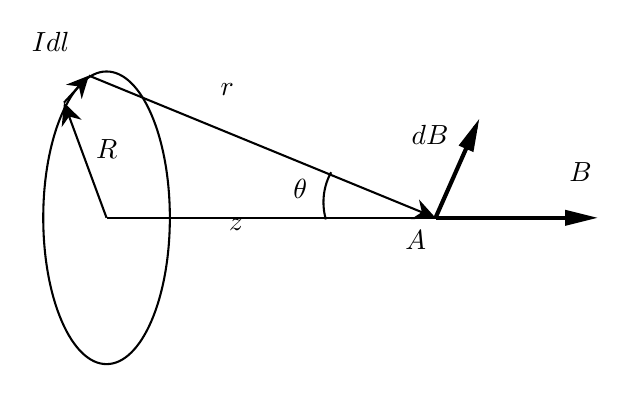
\begin{tikzpicture}[x=0.75pt,y=0.75pt,yscale=-1,xscale=1]
%uncomment if require: \path (0,300); %set diagram left start at 0, and has height of 300

%Shape: Ellipse [id:dp2945629051230668] 
\draw   (84,129.5) .. controls (84,90.56) and (97.66,59) .. (114.5,59) .. controls (131.34,59) and (145,90.56) .. (145,129.5) .. controls (145,168.44) and (131.34,200) .. (114.5,200) .. controls (97.66,200) and (84,168.44) .. (84,129.5) -- cycle ;
%Straight Lines [id:da9466368938913634] 
\draw    (114.5,129.5) -- (273,129.5) ;
%Straight Lines [id:da70947601939368] 
\draw [line width=1.5]    (273,129.5) -- (347,129.5) ;
\draw [shift={(351,129.5)}, rotate = 180] [fill={rgb, 255:red, 0; green, 0; blue, 0 }  ][line width=0.08]  [draw opacity=0] (15.6,-3.9) -- (0,0) -- (15.6,3.9) -- cycle    ;
%Straight Lines [id:da1789396988935933] 
\draw    (114.5,129.5) -- (95.04,76.81) ;
\draw [shift={(94,74)}, rotate = 429.73] [fill={rgb, 255:red, 0; green, 0; blue, 0 }  ][line width=0.08]  [draw opacity=0] (10.72,-5.15) -- (0,0) -- (10.72,5.15) -- (7.12,0) -- cycle    ;
%Straight Lines [id:da5784308387606231] 
\draw    (94,74) -- (103.97,63.2) ;
\draw [shift={(106,61)}, rotate = 492.71] [fill={rgb, 255:red, 0; green, 0; blue, 0 }  ][line width=0.08]  [draw opacity=0] (10.72,-5.15) -- (0,0) -- (10.72,5.15) -- (7.12,0) -- cycle    ;
%Straight Lines [id:da9484257336857925] 
\draw    (106,61) -- (270.22,128.36) ;
\draw [shift={(273,129.5)}, rotate = 202.3] [fill={rgb, 255:red, 0; green, 0; blue, 0 }  ][line width=0.08]  [draw opacity=0] (10.72,-5.15) -- (0,0) -- (10.72,5.15) -- (7.12,0) -- cycle    ;
%Shape: Arc [id:dp508403894077875] 
\draw  [draw opacity=0] (220.15,130.25) .. controls (219.4,127.63) and (219,124.86) .. (219,122) .. controls (219,116.76) and (220.34,111.83) .. (222.71,107.54) -- (249,122) -- cycle ; \draw   (220.15,130.25) .. controls (219.4,127.63) and (219,124.86) .. (219,122) .. controls (219,116.76) and (220.34,111.83) .. (222.71,107.54) ;
%Straight Lines [id:da9544142393607489] 
\draw [line width=1.5]    (273,129.5) -- (292.38,85.66) ;
\draw [shift={(294,82)}, rotate = 473.85] [fill={rgb, 255:red, 0; green, 0; blue, 0 }  ][line width=0.08]  [draw opacity=0] (15.6,-3.9) -- (0,0) -- (15.6,3.9) -- cycle    ;

% Text Node
\draw (108,90.4) node [anchor=north west][inner sep=0.75pt]    {$R$};
% Text Node
\draw (77,38.4) node [anchor=north west][inner sep=0.75pt]    {$Id\ot{l}$};
% Text Node
\draw (168,63.4) node [anchor=north west][inner sep=0.75pt]    {$\ot{r}$};
% Text Node
\draw (203,109.4) node [anchor=north west][inner sep=0.75pt]    {$\theta $};
% Text Node
\draw (172,128.4) node [anchor=north west][inner sep=0.75pt]    {$z$};
% Text Node
\draw (257,134.4) node [anchor=north west][inner sep=0.75pt]    {$A$};
% Text Node
\draw (336,101.4) node [anchor=north west][inner sep=0.75pt]    {$\ot{B}$};
% Text Node
\draw (260,83.4) node [anchor=north west][inner sep=0.75pt]    {$d\ot{B}$};


\end{tikzpicture}
    \end{center}
    \begin{enumerate}[a)]
        \item Có vẻ sẽ đơn giản khi tìm cảm ứng từ của vòng với dòng điện bằng cách sử dụng định luật Biot-Savart và nguyên lí chồng chất. Hình chiếu $z$ của vector từ trường tạo bởi một phần tử bất kì của vòng được tìm thấy là:
    \[\dd B_{z}=\dfrac{\mu_{0}}{4 \pi} \dfrac{I \dd l}{r^{2}} \sin \theta. \tag{1}\]
Sử dụng hình học, ta thu được:
\[
\dd B_{z}=\dfrac{\mu_{0}}{4 \pi} \dfrac{I \dd l}{r^{2}} \dfrac{R}{r}=\dfrac{\mu_{0}}{4 \pi} \dfrac{I \dd l R}{r^{3}}=\dfrac{\mu_{0}}{4 \pi} \dfrac{I \dd l R}{\left(R^{2}+z^{2}\right)^{\frac{3}{2}}}. \tag{2}
\]
Lấy tổng trên tất cả các phần tử của vòng được để cuối cùng nhận được:
\[
B_{z}=\dfrac{\mu_{0}}{4 \pi} \dfrac{I R \cdot 2 \pi R}{\left(R^{2}+z^{2}\right)^{\frac{3}{2}}}=\dfrac{\mu_{0}}{2 \pi} \dfrac{I \cdot \pi R^{2}}{\left(R^{2}+z^{2}\right)^{\frac{3}{2}}}=\dfrac{\mu_{0}}{2 \pi} \dfrac{p_{m}}{\left(R^{2}+z^{2}\right)^{\frac{3}{2}}}. \tag{3}
\]
Tại $z \gg R$ đơn giản hóa biểu thức lại thành:
\[
B_{z}=\dfrac{\mu_{0}}{2 \pi} \dfrac{p_{m}}{\left(R^{2}+z^{2}\right)^{\frac{3}{2}}} \approx \dfrac{\mu_{0}}{2 \pi} \dfrac{p_{m}}{z^{3}}, \tag{4} \label{tu4}
\]
và cuối cùng:
\[\heva{b&=\dfrac{\mu_{0}}{2 \pi}, \\
\beta&=3.}\tag{5} \]
\item 
Rõ ràng là lực Ampe $F_A$ là do thành phần hướng tâm $B_r$ của vector từ trường. Ở một khoảng cách ngắn so với trục, thành phần này có thể được biểu diễn dưới dạng thành phần từ trường dọc trục ($B_z$) bằng cách sử dụng định lí từ thông.
\begin{center}
\tikzset{every picture/.style={line width=0.75pt}} %set default line width to 0.75pt        

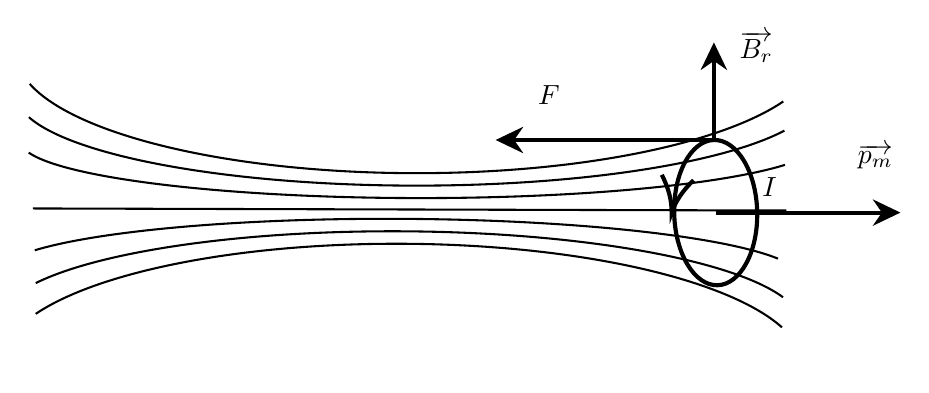
\begin{tikzpicture}[x=0.75pt,y=0.75pt,yscale=-1,xscale=1]
%uncomment if require: \path (0,300); %set diagram left start at 0, and has height of 300

%Shape: Arc [id:dp09724083610265022] 
\draw  [draw opacity=0] (496.56,57.46) .. controls (466.57,77.81) and (398.8,92) .. (320,92) .. controls (230.64,92) and (155.46,73.75) .. (133.49,48.97) -- (320,34) -- cycle ; \draw   (496.56,57.46) .. controls (466.57,77.81) and (398.8,92) .. (320,92) .. controls (230.64,92) and (155.46,73.75) .. (133.49,48.97) ;
%Shape: Arc [id:dp9573942278688676] 
\draw  [draw opacity=0] (497.09,71.52) .. controls (467.39,87.1) and (399.28,98) .. (320,98) .. controls (230.13,98) and (154.6,84) .. (133.12,65.04) -- (320,54) -- cycle ; \draw   (497.09,71.52) .. controls (467.39,87.1) and (399.28,98) .. (320,98) .. controls (230.13,98) and (154.6,84) .. (133.12,65.04) ;
%Shape: Arc [id:dp5398400734661393] 
\draw  [draw opacity=0] (497.38,88) .. controls (466.83,97.44) and (399.79,104) .. (322,104) .. controls (228.9,104) and (151.19,94.61) .. (133.02,82.11) -- (322,76.5) -- cycle ; \draw   (497.38,88) .. controls (466.83,97.44) and (399.79,104) .. (322,104) .. controls (228.9,104) and (151.19,94.61) .. (133.02,82.11) ;
%Shape: Arc [id:dp5931355655659283] 
\draw  [draw opacity=0] (136.4,159.79) .. controls (166.42,139.54) and (234.33,125.63) .. (313.23,126.01) .. controls (398.2,126.41) and (470.27,143.25) .. (495.93,166.29) -- (312.96,184) -- cycle ; \draw   (136.4,159.79) .. controls (166.42,139.54) and (234.33,125.63) .. (313.23,126.01) .. controls (398.2,126.41) and (470.27,143.25) .. (495.93,166.29) ;
%Shape: Arc [id:dp18584702804365694] 
\draw  [draw opacity=0] (136.42,144.95) .. controls (166.88,129.89) and (234.18,119.63) .. (312.26,120) .. controls (398.87,120.41) and (472.09,133.76) .. (496.44,151.79) -- (312.05,164) -- cycle ; \draw   (136.42,144.95) .. controls (166.88,129.89) and (234.18,119.63) .. (312.26,120) .. controls (398.87,120.41) and (472.09,133.76) .. (496.44,151.79) ;
%Shape: Arc [id:dp843366810007487] 
\draw  [draw opacity=0] (135.94,129.15) .. controls (166.63,119.86) and (233.81,113.63) .. (311.71,114) .. controls (395.9,114.39) and (467.49,122.38) .. (494.01,133.18) -- (311.58,141.5) -- cycle ; \draw   (135.94,129.15) .. controls (166.63,119.86) and (233.81,113.63) .. (311.71,114) .. controls (395.9,114.39) and (467.49,122.38) .. (494.01,133.18) ;
%Straight Lines [id:da0825312466176309] 
\draw    (498,110) -- (135,109) ;
%Shape: Ellipse [id:dp154624595511056] 
\draw  [line width=1.5]  (463.14,76.01) .. controls (474.19,75.74) and (483.52,91.19) .. (483.99,110.51) .. controls (484.47,129.84) and (475.9,145.72) .. (464.86,145.99) .. controls (453.81,146.26) and (444.48,130.81) .. (444.01,111.49) .. controls (443.53,92.16) and (452.1,76.28) .. (463.14,76.01) -- cycle ;
\draw  [line width=1.5]  (453.33,95.42) .. controls (448.11,100.37) and (444.6,105.61) .. (442.77,111.14) .. controls (442.89,105.32) and (441.32,99.21) .. (438.04,92.8) ;
%Straight Lines [id:da9522131982799203] 
\draw [line width=1.5]    (464,111) -- (549,111) ;
\draw [shift={(553,111)}, rotate = 180] [fill={rgb, 255:red, 0; green, 0; blue, 0 }  ][line width=0.08]  [draw opacity=0] (13.4,-6.43) -- (0,0) -- (13.4,6.44) -- (8.9,0) -- cycle    ;
%Straight Lines [id:da050548300708038396] 
\draw [line width=1.5]    (463.14,76.01) -- (362,76.01) ;
\draw [shift={(358,76.01)}, rotate = 360] [fill={rgb, 255:red, 0; green, 0; blue, 0 }  ][line width=0.08]  [draw opacity=0] (13.4,-6.43) -- (0,0) -- (13.4,6.44) -- (8.9,0) -- cycle    ;
%Straight Lines [id:da5809933990248567] 
\draw [line width=1.5]    (463.14,76.01) -- (463.14,33) ;
\draw [shift={(463.14,29)}, rotate = 450] [fill={rgb, 255:red, 0; green, 0; blue, 0 }  ][line width=0.08]  [draw opacity=0] (13.4,-6.43) -- (0,0) -- (13.4,6.44) -- (8.9,0) -- cycle    ;

% Text Node
\draw (531,76.4) node [anchor=north west][inner sep=0.75pt]    {$\overrightarrow{p_{m}}$};
% Text Node
\draw (377,48.4) node [anchor=north west][inner sep=0.75pt]    {$\ot{F}$};
% Text Node
\draw (485,92.4) node [anchor=north west][inner sep=0.75pt]    {$I$};
% Text Node
\draw (474,22.4) node [anchor=north west][inner sep=0.75pt]    {$\overrightarrow{B_{r}}$};
\end{tikzpicture}
\end{center}
Chọn bề mặt có dạng hình trụ mỏng có trục trùng với trục của từ trường, sau đó viết biểu thức tổng đại số từ thông xuyên qua các bề mặt và cho nó bằng không, ta thu được:
\[
B_{z}(z+\dd z) \cdot \pi r^{2}-B_{z}(z) \cdot \pi r^{2}+B_{r} \cdot 2 \pi r \dd z=0. \tag{6}
\]
Do đó, phương trình rút gọn lại thành:
\[
B_{r}=-\dfrac{r}{2} \dfrac{\dd B_{z}}{\dd z}. \tag{7}
\]
Sử dụng định luật Ampe, ta dễ dàng viết được phương trình của lực tác dụng lên vòng:
\[
F=I B_{r} 2 \pi r=-I \dfrac{r}{2} \dfrac{\dd B_{z}}{\dd z} 2 \pi r=-p_{m} \dfrac{\dd B_{z}}{\dd z}. \tag{8} \label{tu8}
\]
\end{enumerate}
\item \begin{enumerate}[a)]
    \item Tần số dao động được xác định theo công thức về tần số dao động của con lắc lò xo:
\[\omega_{0}=\sqrt{\dfrac{k}{m}}. \tag{9}\]
\item Cơ chế phản hồi từ đĩa đến nam châm được mô tả như sau: khi nam châm chuyển động, điện trường xoáy được tạo ra trong đĩa làm phát sinh dòng điện xoáy. Từ trường của các dòng điện xoáy đó là nguồn lực tác dụng lên nam châm. Để tính toán từ trường tạo ra bởi dòng điện xoáy trong đĩa, cần lưu ý rằng kích thước của đĩa nhỏ so với khoảng cách đến nam châm, vì vậy đĩa cũng có thể được coi là một lưỡng cực từ. Do đó, chỉ cần tìm moment từ cảm ứng của đĩa là đủ, và sau đó sử dụng công thức (\ref{tu4}) để tính trường cảm ứng.
\begin{center}


\tikzset{every picture/.style={line width=0.75pt}} %set default line width to 0.75pt        

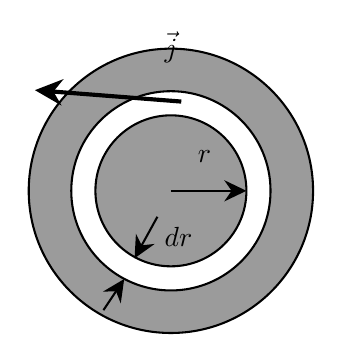
\begin{tikzpicture}[x=0.75pt,y=0.75pt,yscale=-1,xscale=1]
%uncomment if require: \path (0,300); %set diagram left start at 0, and has height of 300

%Shape: Circle [id:dp5627498650118721] 
\draw  [fill={rgb, 255:red, 155; green, 155; blue, 155 }  ,fill opacity=1 ] (214,135.5) .. controls (214,97.67) and (244.67,67) .. (282.5,67) .. controls (320.33,67) and (351,97.67) .. (351,135.5) .. controls (351,173.33) and (320.33,204) .. (282.5,204) .. controls (244.67,204) and (214,173.33) .. (214,135.5) -- cycle ;
%Shape: Circle [id:dp35534083435887376] 
\draw  [fill={rgb, 255:red, 255; green, 255; blue, 255 }  ,fill opacity=1 ] (234.5,135.5) .. controls (234.5,108.99) and (255.99,87.5) .. (282.5,87.5) .. controls (309.01,87.5) and (330.5,108.99) .. (330.5,135.5) .. controls (330.5,162.01) and (309.01,183.5) .. (282.5,183.5) .. controls (255.99,183.5) and (234.5,162.01) .. (234.5,135.5) -- cycle ;
%Shape: Circle [id:dp29382362351556024] 
\draw  [fill={rgb, 255:red, 155; green, 155; blue, 155 }  ,fill opacity=1 ] (246.13,135.5) .. controls (246.13,115.41) and (262.41,99.13) .. (282.5,99.13) .. controls (302.59,99.13) and (318.88,115.41) .. (318.88,135.5) .. controls (318.88,155.59) and (302.59,171.88) .. (282.5,171.88) .. controls (262.41,171.88) and (246.13,155.59) .. (246.13,135.5) -- cycle ;
%Straight Lines [id:da025040465706037685] 
\draw    (250,193) -- (258.34,180.5) ;
\draw [shift={(260,178)}, rotate = 483.69] [fill={rgb, 255:red, 0; green, 0; blue, 0 }  ][line width=0.08]  [draw opacity=0] (10.72,-5.15) -- (0,0) -- (10.72,5.15) -- (7.12,0) -- cycle    ;
%Straight Lines [id:da48334265372989726] 
\draw    (276,148) -- (266.45,165.37) ;
\draw [shift={(265,168)}, rotate = 298.81] [fill={rgb, 255:red, 0; green, 0; blue, 0 }  ][line width=0.08]  [draw opacity=0] (10.72,-5.15) -- (0,0) -- (10.72,5.15) -- (7.12,0) -- cycle    ;
%Straight Lines [id:da47382347877822695] 
\draw    (282.5,135.5) -- (315.88,135.5) ;
\draw [shift={(318.88,135.5)}, rotate = 180] [fill={rgb, 255:red, 0; green, 0; blue, 0 }  ][line width=0.08]  [draw opacity=0] (10.72,-5.15) -- (0,0) -- (10.72,5.15) -- (7.12,0) -- cycle    ;
%Straight Lines [id:da7855177903566417] 
\draw [line width=1.5]    (287.5,92.5) -- (220.99,87.31) ;
\draw [shift={(217,87)}, rotate = 364.46000000000004] [fill={rgb, 255:red, 0; green, 0; blue, 0 }  ][line width=0.08]  [draw opacity=0] (13.4,-6.43) -- (0,0) -- (13.4,6.44) -- (8.9,0) -- cycle    ;

% Text Node
\draw (278,151.4) node [anchor=north west][inner sep=0.75pt]    {$dr$};
% Text Node
\draw (294,114.4) node [anchor=north west][inner sep=0.75pt]    {$r$};
% Text Node
\draw (278,57.4) node [anchor=north west][inner sep=0.75pt]    {$\vec{j}$};


\end{tikzpicture}
\end{center}
Chúng ta hãy xem xét một vòng mỏng bán kính $r$ và chiều dày $\dd r$. Cường độ của điện trường xoáy trong vòng này được tìm thấy từ định luật cảm ứng Faraday là:
\[
2 \pi r E=-\pi r^{2} \dfrac{\dd B_{z}}{\dd t} \Rightarrow E=-\dfrac{r}{2} \dfrac{\dd B_{z}}{\dd t}. \tag{10} \label{tu10}
\]
Ở đây giả thiết rằng trong toàn bộ đĩa, người ta có thể bỏ qua sự biến thiên của thành phần dọc theo  trục của từ trường do nam châm tạo ra, cũng được xác định theo công thức (\ref{tu4}). Do đó, nếu tọa độ nam châm là $x$, thì từ trường tại vị trí của nó thu được là:
\[
B_{z}=\dfrac{\mu_{0}}{2 \pi} \dfrac{p_{m}}{(z-x)^{3}}. \tag{11}
\]
Theo công thức ở (\ref{tu10}), điện trường xoáy ở một điểm trên đĩa có bán kính $r$ là:
\[
E=-\dfrac{r}{2} \dfrac{\dd B_{z}}{\dd t}=-\dfrac{r}{2} \cdot \dfrac{3 \mu_{0}}{2 \pi} \dfrac{p_{m}}{(z-x)^{4}} \dfrac{\dd x}{\dd t} \approx-\dfrac{3 \mu_{0}}{4 \pi} r \dfrac{p_{m}}{z^{4}} v. \tag{12}
\]
Ở đây ta lưu ý dùng tới dữ kiện $x \ll z$.\\
Theo định luật Ohm, mật độ dòng chạy trong đĩa là:
\[
j=\dfrac{1}{\rho} E. \tag{13}
\]
Cường độ dòng điện chạy trong vành có độ rộng $\dd r$ là: $\dd I=jh\dd r$, từ đó moment từ của một vành này là:
\[
\dd p_{m}^{\prime}=\pi r^{2} \dd I=\pi r^{2} j \dd r \cdot h=-\pi r^{2} \dd r \cdot h \dfrac{3 \mu_{0}}{4 \pi \rho} r \dfrac{p_{m}}{z^{4}} v=-\dfrac{3 \mu_{0}}{4 \rho} \dfrac{p_{m}}{z^{4}} h v r^{3} \dd r. \tag{14}
\]
Tích phân trên toàn bộ đĩa, người ta thu được tổng moment từ của nó là:
\[
p_{m}^{\prime}=-\dfrac{3 \mu_{0}}{4 \rho} \dfrac{p_{m}}{z^{4}} h v \int_{0}^{R} r^{3} \dd r=-\dfrac{3 \mu_{0}}{16 \rho} \dfrac{p_{m}}{z^{4}} h R^{4} v. \tag{15}
\]
Để tính lực tác dụng lên nam châm, ta áp dụng biểu thức (\ref{tu8}), trong đó từ trường của đĩa gây ra đã tính được từ biểu thức (\ref{tu4}). Từ đó ta thu được phương trình:
\begin{align*}
F&=-p_{m} \dfrac{\dd B_{z}}{\dd z}=-p_{m} \dfrac{\dd}{\dd z}\left(\dfrac{\mu_{0}}{2 \pi} \dfrac{p_{m}^{\prime}}{z^{3}}\right)=\dfrac{3 \mu_{0}}{2 \pi} \dfrac{p_{m} p_{m}^{\prime}}{z^{4}}\\
&=-\dfrac{3 \mu_{0}}{2 \pi} \dfrac{p_{m}}{z^{4}} \dfrac{3 \mu_{0}}{16 \rho} \dfrac{p_{m}}{z^{4}} h R^{4} v=-\dfrac{9}{32} \dfrac{\mu_{0}^{2} p_{m}^{2}}{\pi \rho z^{8}} h R^{4} v. \tag{16} \label{tu16}
\end{align*}
Phương trình chuyển động của nam châm dưới tác dụng của đĩa có dạng:
\[
m x^{\prime \prime}=-k x-b x^{\prime}, \tag{17}
\]
trong đó $b=\dfrac{9}{32} \dfrac{\mu_{0}^{2} p_{m}^{2}}{\pi \rho z^{8}} h R^{4}$ là hệ số được xác định trong công thức (\ref{tu16}).
\item Sử dụng nghiệm của phương trình dao động tắt dần được cho trong công thức bài toán, ta nhận được:
\[
\omega=\sqrt{\omega_{0}^{2}-\beta^{2}}=\omega_{0}\left(1-\dfrac{\beta^{2}}{\omega_{0}^{2}}\right)^{\frac{1}{2}} \approx \omega_{0}\left(1-\dfrac{\beta^{2}}{2 \omega_{0}^{2}}\right), \tag{18}
\]
trong đó $\beta= \dfrac{b}{2m}$. Từ đây, ta tính được sự thay đổi tần số tương đối là:
\[
\dfrac{\Delta \omega}{\omega_{0}}=-\dfrac{\beta^{2}}{2 \omega_{0}^{2}}=-\dfrac{1}{2 k m}\left(\dfrac{9}{64} \dfrac{\mu_{0}^{2} p_{m}^{2}}{\pi \rho z^{8}} h R^{4}\right)^{2}. 
\]
\item Do đó, thời gian suy giảm đặc trưng bằng:
\[
\tau=\dfrac{1}{\beta}=\dfrac{2 m}{b}=\dfrac{64 m \pi \rho z^{8}}{9 \mu_{0}^{2} p_{m}^{2} h R^{4}}.
\]
Theo định luật Joule, công suất mất nhiệt tức thời trong đĩa được suy ra là:
\[
P=\int \rho j^{2} \dd V=\int_{0}^{R} \rho\left(\dfrac{3 \mu_{0} p_{m} v}{4 \pi z^{8} \rho} r\right)^{2} h 2 \pi r \dd r=\dfrac{9 h \mu_{0}^{2} p_{m}^{2} R^{4}}{32 \pi z^{8} \rho} v^{2}.
\]
Và nó bằng tích của lực ở phương trình (\ref{tu16}) với tốc độ $v$ của nam châm.
\end{enumerate}    
\end{enumerate}
\begin{center}
\textbf{Phần II: Điện tích}
\end{center}
\begin{enumerate}[1)]
\item \textbf{Giới thiệu lí thuyết:}
\begin{enumerate}[a)]
    \item Điện trường của lưỡng cực được tính theo nguyên lí chồng chất: 
\begin{align*}
E=E_{+}-E_{-}&=\dfrac{q}{4 \pi \varepsilon_{0}\left(z-\dfrac{l}{2}\right)^{2}}-\dfrac{q}{4 \pi \varepsilon_{0}\left(z+\dfrac{l}{2}\right)^{2}}\\
&=\dfrac{q \cdot 2 z l}{4 \pi \varepsilon_{0}\left(z^{2}-\left(\dfrac{l}{2}\right)^{2}\right)^{2}}=\dfrac{z p_{e}}{2 \pi \varepsilon_{0}\left(z^{2}-\left(\dfrac{l}{2}\right)^{2}\right)^{2}}. \tag{19}
    \end{align*}
    Với $z\ll l$, đơn giản hóa biểu thức thành:
    \[
E=\dfrac{z p_{e}}{2 \pi \varepsilon_{0}\left(z^{2}-\left(\dfrac{l}{2}\right)^{2}\right)^{2}}=\dfrac{1}{2 \pi \varepsilon_{0}} \dfrac{p_{e}}{z^{3}}. \tag{20}
\]
Do đó:
\[\heva{a&=\dfrac{1}{2 \pi \varepsilon_0},\\
    \alpha&=3.}\tag{21} \]
\end{enumerate}
\item \textbf{Dao động của quả cầu tích điện.}
\begin{enumerate}[a)]
    \item Chúng ta hãy suy ra một biểu thức cho lực tác dụng lên quả cầu bởi đĩa.\\
    Điện trường bên trong của đĩa là bằng không. Điện trường $E_0$ do điện tích $q$ tạo ra mật độ điện tích $\pm \sigma$ trên bề mặt đĩa, khi đó nó tạo ra điện trường $\ot{E^\prime}$ có độ lớn bằng nhưng ngược hướng với điện trường của điện tích điểm. Cho rằng kích thước của đĩa nhỏ so với sự phân bố điện tích, có thể bỏ qua sự biến thiên vector điện trường $E_0$ trên đĩa. Do đó, điện trường phải là đều và mật độ điện tích mặt của các điện tích cảm ứng phải được coi là không đổi.\\
    Điện trường do điện tích điểm gây ra có biểu thức:
    \[E_0=\dfrac{q}{4 \pi \varepsilon_0 z^2}.\]
    Điện trường gây ra bởi sự phân bố điện tích mặt là:
    \[
E^{\prime}=\dfrac{\sigma}{\varepsilon_{0}}.
\]
Như đã nói ở trên thì hai điện trường trên phải bằng nhau, do đó:
\[
\sigma^{\prime}=\dfrac{q}{4 \pi z^{2}}.
\]
Do đó độ lớn điện tích trên mặt đĩa là:
\[ q^\prime=\sigma^ \prime S =\dfrac{qS}{4 \pi z^2}, \]
trong đó $S=\pi R^2$ là diện tích của đĩa. Vì vậy, ta có thể coi như đĩa là một lưỡng cực điện cho bởi:
\[
p_{e}^{\prime}=q^{\prime} h=\dfrac{q S h}{4 \pi z^{2}}=\dfrac{q}{4 \pi z^{2}} V. \tag{22}
\]
Lực tác dụng lên quả cầu là:
\[
F=q E=q \dfrac{1}{2 \pi \varepsilon_{0}} \dfrac{p_{e}^{\prime}}{z^{3}}=\dfrac{q^{2}}{8 \pi^{2} \varepsilon_{0} z^{5}} V. \tag{23}
\]
Vì quả cầu chuyển động, trong công thức cuối cùng $z$ nên được thay bằng $z-x$. Cho rằng $x \ll z$, biểu thức kết quả cho lực đơn giản hóa thành:
\[
F=\dfrac{q^{2} V}{8 \pi^{2} \varepsilon_{0}(z-x)^{5}}=\dfrac{q^{2} V}{8 \pi^{2} \varepsilon_{0} z^{5}}\left(1-\dfrac{x}{z}\right)^{-5} \approx \dfrac{q^{2} V}{8 \pi^{2} \varepsilon_{0} z^{5}}+5 \dfrac{q^{2} V}{8 \pi^{2} \varepsilon_{0} z^{6}} x. \tag{24} \label{tu24}
\]
Phương trình chuyển động của quả cầu trong trường hợp này có dạng:
\[
m x^{\prime \prime}=-k x+\dfrac{q^{2} V}{8 \pi^{2} \varepsilon_{0} z^{5}}+5 \dfrac{q^{2} V}{8 \pi^{2} \varepsilon_{0} z^{6}} x. \tag{25}
\]
Số hạng đầu tiên trong phương trình (\ref{tu24}) dẫn đến dịch chuyển bổ sung của vị trí cân bằng, trong khoảng giá trị gần đúng được sử dụng bằng:
\[
k \Delta x=\dfrac{q^{2} V}{8 \pi^{2} \varepsilon_{0} z^{5}} \Rightarrow \Delta x=\dfrac{q^{2} V}{8 \pi^{2} \varepsilon_{0} z^{5} k}. \tag{26}
\]
\item Số hạng thứ hai trong phương trình (\ref{tu25}) xác định sự thay đổi tần số của dao động là:
\[
\omega=\sqrt{\dfrac{k}{m}-\dfrac{5 q^{2} V}{8 \pi^{2} \varepsilon_{0} z^{6} m}}=\sqrt{\omega_{0}^{2}-\dfrac{5 q^{2} V}{8 \pi^{2} \varepsilon_{0} z^{6} m}} \approx \omega_{0}\left(1-\dfrac{5 q^{2} V}{16 \pi^{2} \varepsilon_{0} z^{6} m}\right), \tag{27}
\]
mang lại sự thay đổi tần số tương đối:
\[
\dfrac{\Delta \omega}{\omega_{0}}=-\dfrac{5 q^{2} V}{16 \pi^{2} \varepsilon_{0} z^{6} m}. \tag{28}
\]
\item Mật độ điện tích bề mặt $\sigma$ trên mặt đĩa thay đổi do dòng điện trong đĩa được xác định bởi cường độ điện trường trong đĩa ($\dot{\sigma}=j=\dfrac{E}{\rho}$). Điện trường trong đĩa do quả cầu tạo ra:
\[
E_{1}=\dfrac{1}{4 \pi \varepsilon_{0}} \dfrac{q}{(z-x)^{2}} \approx \dfrac{q}{4 \pi \varepsilon_{0} z^{2}}\left(1+2 \dfrac{x}{z}\right),
\]
và điện trường hướng ngược lại do các điện tích gây ra:
\[
E_{2}=-\dfrac{\sigma}{\varepsilon_{0}}.
\]
Định luật Ohm $E_1+E_2=\rho j$ có thể viết lại thành:
\[
\dfrac{q}{4 \pi \varepsilon_{0} z^{2}}\left(1+2 \dfrac{x}{z}\right)-\dfrac{\sigma}{\varepsilon_{0}}=\rho j.
\]
Bây giờ cho $\dot{\sigma}=j$ và $p=\sigma S h= \sigma V \ (V=\pi R^2 h)$ ta nhận được phương trình cuối cùng:
\[
\varepsilon_{0} \rho \dot{p}+p=\dfrac{q V}{4 \pi z^{2}}\left(1+2 \dfrac{x}{z}\right).
\]
\item \[
R=\rho \dfrac{h}{s},\quad C=\dfrac{\varepsilon_{0} S}{h},\quad \tau=R C=\varepsilon_{0} \rho.
\]
\item \[
\dfrac{2 \pi}{\omega} \gg \varepsilon_{0} \rho \ \text { hoặc } \  \varepsilon_{0} \rho \omega \ll 1.
\]
\item Dao động điều hòa, tỉ số giữa biên độ của $\varepsilon_{0} \rho \dot{p}$ với biên độ của $p$ bằng $\varepsilon_{0} \rho \omega$, tức là nó rất nhỏ. Do đó, xấp xỉ bằng không trong phương trình:
\[
\varepsilon_{0} \rho \dot{p}+p=\dfrac{q V}{4 \pi z^{2}}\left(1+2 \dfrac{x}{z}\right),
\]
ta có thể bỏ qua số hạng đầu:
\[
p=\dfrac{q V}{4 \pi z^{2}}\left(1+2 \dfrac{x}{z}\right) \ \text { và } \ \dot{p}=\dfrac{q V}{2 \pi z^{3}} v.
\]
Ta tìm được $\dot{p}$ từ biểu thức gốc:
\[
p=\dfrac{q V}{4 \pi z^{2}}\left(1+2 \dfrac{x}{z}\right)-\varepsilon_{0} \rho \dot{p}=\dfrac{q V}{4 \pi z^{2}}\left(1+2 \dfrac{x}{z}\right)-\varepsilon_{0} \rho \dfrac{q V}{2 \pi z^{3}} v.
\]
Lưu ý rằng giải pháp sử dụng giản đồ vector cũng có thể thực hiện được.
\item Lực do đĩa tác dụng lên quả cầu là:
\begin{align*}
F &= \dfrac{p}{2 \pi \varepsilon_{0}(z-x)^{3}} q=\dfrac{q}{2 \pi \varepsilon_{0} z^{3}}\left(1+3 \dfrac{x}{z}\right)\left[\dfrac{q V}{4 \pi z^{2}}\left(1+2 \dfrac{x}{z}\right)-\varepsilon_{0} \rho \dfrac{q V}{2 \pi z^{3}} v\right]\\
 &= \dfrac{q^{2} R^{2} h}{8 \pi \varepsilon_{0} Z^{6}}\left[(z+5 x)-2 \varepsilon_{0} \rho v\right].
\end{align*}
Do đó, phương trình chuyển động của quả cầu được viết dưới dạng:
\[
m x^{\prime \prime}=-k x+\dfrac{q^{2} R^{2} h}{8 \pi \varepsilon_{0} z^{6}}\left[(z+5 x)-2 \varepsilon_{0} \rho v\right],
\]
hoặc
\[
m x^{\prime \prime}+\dfrac{q^{2} \rho R^{2} h}{4 \pi z^{6}} x^{\prime}+\left[k-\dfrac{5 q^{2} R^{2} h}{8 \pi \varepsilon_{0} z^{6}}\right] x=\dfrac{q^{2} R^{2} h}{8 \pi \varepsilon_{0} z^{5}}.
\]
\item \[
b=\dfrac{q^{2} \rho R^{2} h}{4 \pi z^{6}}, \quad \beta=\dfrac{b}{2 m}=\dfrac{q^{2} \rho R^{2} h}{8 \pi z^{6} m}, \quad \tau=\dfrac{1}{\beta}=\dfrac{8 \pi z^{6} m}{q^{2} \rho R^{2} h}.
\]
\item Theo định luật Joule, nhiệt sinh ra tức thời trong đĩa:
\[
P=j^{2} \rho V=\left(\dfrac{q v}{2 \pi z^{3}}\right)^{2} \rho V=\dfrac{q^{2} \rho R^{2} h}{4 \pi z^{6}} v^{2}=b v^{2},
\]
nó tiếp tục bằng công suất của lực $(F=-bv)$.
\end{enumerate}
\end{enumerate}
\end{loigiai}


\begin{vd}[Phản ứng nhiệt hạch nhân tạo (Kiểm soát được)]
Trong bài làm, bạn có thể sẽ cần sử dụng các hằng số vật lí sau:
\begin{itemize}
    \item Hằng số Boltzmann: $k_{B}=1,381\times 10^{-23}~ \mathrm{J\cdot K^{-1}}$.
    \item Giá trị điện tích của electron: $e=1,602\times 10^{-19} ~\mathrm{C}$.
    \item Khối lượng của electron: $m_{e}=9,109\times 10^{-31}~\mathrm{kg}$.
    \item Hằng số Plank: $h=6,626\times 10^{-34} ~\mathrm{m^2\cdot kg \cdot s^{-1}}$.
    \item Độ điện thẩm của chân không: $\varepsilon_0=8,854\times 10^{-12}  ~\mathrm{F\cdot m^{-1}}$.
\end{itemize}
Phản ứng nhiệt hạch là phản ứng kết hợp hai hạt nhân nhẹ để tạo thành một hạt nhân nặng hơn đồng thời sẽ có một phần năng lượng tỏa ra dưới dạng nhiệt. Một ví dụ cho phản ứng trên là lấy hạt ``Deuterium'' (gồm một hạt neutron và một hạt proton, kí hiệu là $D$) cho phản ứng với hạt ``Tritium'' (gồm hai hạt neutron và một hạt proton, kí hiệu là $T$) thì sẽ cho sản phẩm là một hạt $\alpha$, một hạt neutron và $14~\mathrm{MeV}$. Mặc dù con người đã nghiên cứu ra cách để khơi mào phản ứng nhiệt hạch trong những quả bom nguyên tử, thế nhưng họ vẫn phải chật vật đấu tranh để có thể thành công trong lĩnh vực nhiệt hạch nhân tạo (kiểm soát được), hay nói một cách khác là để có thể kiểm soát hoàn toàn được phản ứng nhiệt hạch với mục tiêu đặt ra là lượng nhiệt tỏa ra có thể sử dụng để vận hành các nhà máy điện. Phản ứng khả thi nhất trong tất cả các phản ứng nhiệt hạch nhân tạo (kiểm soát được) chính là phản ứng giữa hai hạt ``Deuterium'' và ``Tritium'' được nêu ở trên, và chính phản ứng đó sẽ được đề cập và giải quyết trong bài toán này.
\begin{enumerate}[{Phần }A.]
    \item \textbf{Tổng quan:}\\
Sau đây, chúng ta sẽ biểu diễn nhiệt độ theo $\mathrm{eV}$; một cách biểu diễn phổ biến khi ở nhiệt độ cao. $1~\mathrm{eV}$ tương ứng với một nhiệt độ $T$ nhất định mà tại đó năng lượng nhiệt $k_{B}T$ bằng thế năng của một electron với điện thế $V=1~\mathrm{V}$.\\
Trong một nhà máy điện, năng lượng do phản ứng nhiệt hạch tỏa ra phải lớn hơn tổng năng lượng bị mất đi. Điều đó cho thấy rằng lò phản ứng $D-T$ (thiết bị mà ở đó phản ứng nhiệt hạch nhân tạo xảy ra) được thiết kế tối ưu, nhiệt độ của hạt nhân ``Deuterium'' và ``Tritium'' phải là $T_0=14~\mathrm{keV}$ trong khi đó tích số giữa mật độ phân bố phân tử $n$ (số phân tử trên một đơn vị thể tích) và thời gian ``giam'' $\tau$ (khoảng thời gian mà trong đó mật độ $n$ có giá trị gần như không đổi) phải không được bé hơn $2\times 10^{20} ~\mathrm{s/m^3}$; điều kiện này được biết đến trong những tiêu chuẩn của Lawson (the Lawson criterion). Và thử thách kỹ thuật lớn nhất là phải ``giam'' được trạng thái plasma nóng đủ lâu.\\
Hãy biểu diễn nhiệt độ $T_0$ theo Kelvins.

    \item \textbf{Tokamak:}\\
Trong những thiết kế của lò phản ứng hạt nhân, thiết kế nổi tiếng và phổ biến nhất chính là tokamak. Trong tokamak, các hạt được tích điện di chuyển dọc theo các đường sức từ và bị giữ lại bởi vì các đường sức bị giới hạn trong một khoảng không gian nhất định. Theo định tính, các đường sức từ trong trường hợp này có cùng hình dạng với trong trường hợp mà ở đó các được sức từ được tạo ra bởi dòng điện thẳng dài vô hạn đâm xuyên qua vòng tròn có dòng điện chạy qua khép kín (đồng trục với đường thẳng đi qua tâm của các vòng tròn ấy). Và sau đây, bạn hãy cung cấp các bản phác họa trong không gian ba chiều như trong hình.
\begin{center}
    \tikzset{every picture/.style={line width=0.75pt}} %set default line width to 0.75pt        

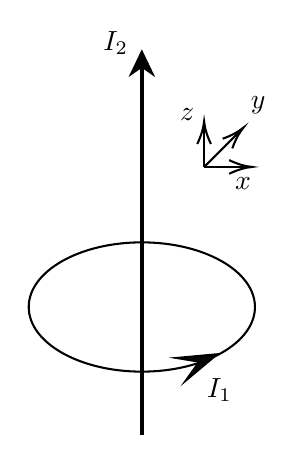
\begin{tikzpicture}[x=0.75pt,y=0.75pt,yscale=-1,xscale=1]
%uncomment if require: \path (0,300); %set diagram left start at 0, and has height of 300

%Straight Lines [id:da9727042378370543] 
\draw [line width=1.5]    (290,57.33) -- (290,239.33) ;
\draw [shift={(290,53.33)}, rotate = 90] [fill={rgb, 255:red, 0; green, 0; blue, 0 }  ][line width=0.08]  [draw opacity=0] (13.4,-6.43) -- (0,0) -- (13.4,6.44) -- (8.9,0) -- cycle    ;
%Shape: Ellipse [id:dp38669151961851567] 
\draw   (235.5,177.48) .. controls (235.5,160.28) and (259.9,146.33) .. (290,146.33) .. controls (320.1,146.33) and (344.5,160.28) .. (344.5,177.48) .. controls (344.5,194.68) and (320.1,208.62) .. (290,208.62) .. controls (259.9,208.62) and (235.5,194.68) .. (235.5,177.48) -- cycle ;
\draw  [fill={rgb, 255:red, 7; green, 7; blue, 7 }  ,fill opacity=1 ][line width=0.75]  (306.81,202.03) -- (326.28,200.25) -- (311.29,212.8) -- (317.67,203.83) -- cycle ;
%Straight Lines [id:da9784557873509063] 
\draw    (320,110) -- (341,110) ;
\draw [shift={(343,110)}, rotate = 180] [color={rgb, 255:red, 0; green, 0; blue, 0 }  ][line width=0.75]    (10.93,-3.29) .. controls (6.95,-1.4) and (3.31,-0.3) .. (0,0) .. controls (3.31,0.3) and (6.95,1.4) .. (10.93,3.29)   ;
%Straight Lines [id:da27017101324520354] 
\draw    (320,110) -- (320,90) ;
\draw [shift={(320,88)}, rotate = 450] [color={rgb, 255:red, 0; green, 0; blue, 0 }  ][line width=0.75]    (10.93,-3.29) .. controls (6.95,-1.4) and (3.31,-0.3) .. (0,0) .. controls (3.31,0.3) and (6.95,1.4) .. (10.93,3.29)   ;
%Straight Lines [id:da648779265851062] 
\draw    (320,110) -- (337.59,92.41) ;
\draw [shift={(339,91)}, rotate = 495] [color={rgb, 255:red, 0; green, 0; blue, 0 }  ][line width=0.75]    (10.93,-3.29) .. controls (6.95,-1.4) and (3.31,-0.3) .. (0,0) .. controls (3.31,0.3) and (6.95,1.4) .. (10.93,3.29)   ;

% Text Node
\draw (320,210.4) node [anchor=north west][inner sep=0.75pt]    {$I_{1}$};
% Text Node
\draw (270,43.4) node [anchor=north west][inner sep=0.75pt]    {$I_{2}$};
% Text Node
\draw (333.5,113.4) node [anchor=north west][inner sep=0.75pt]    {$x$};
% Text Node
\draw (341,74.4) node [anchor=north west][inner sep=0.75pt]    {$y$};
% Text Node
\draw (307,80.4) node [anchor=north west][inner sep=0.75pt]    {$z$};


\end{tikzpicture}
\end{center}
 \begin{enumerate}[1)]
     \item Phác họa các đường sức từ tạo ra bởi dòng điện thẳng dài vô hạn.
     \item Phác họa các đường sức từ tạo ra bởi vòng tròn khép kín có dòng điện chạy qua.
     \item Phác họa đường sức từ tạo ra bởi dòng điện thẳng dài vô hạn đâm xuyên đồng tâm với trục của dòng điện tròn khép kín, bắt đầu từ khoảng cách nhỏ tính từ dòng điện tròn.
     \item Cho hình dạng dòng điện giống như trên, phác thảo đường sức từ bắt đầu từ một khoảng cách nhỏ tính từ dòng điện thẳng.
 \end{enumerate}   
    \item \textbf{Cold Fusion} (Hợp hạch lạnh)\textbf{:}\\
``Hợp hạch lạnh'' là một quá trình ``muon $-$ catalytic fusion'' (phản ứng nhiệt hạch được đẩy nhanh bằng các chất xúc tác muon) mà trong đó một electron trong phân tử Hidro (phân tử mà có thể bao gồm một hạt nhân Deuterium và một hạt nhân Tritium) được thay thế bởi một muon. Muon, có khối lượng lớn hơn $207$ lần so với một electron, sẽ làm cho các  các hạt nhân trong phân tử xích lại gần nhau hơn, từ đó làm tăng xác suất xảy sự dung hợp. Ý tưởng về ``catalytic fusion'' (phản ứng nhiệt hạch được đẩy nhanh bằng các chất xúc tác) được đề xuất vào năm $1947$ $-$ $48$ bởi  A. Sakharov và F.C. Frank, và dẫn tới sự bùng nổ của các cuộc nghiên cứu ngắn hạn vào năm $1989$ sau một bài báo cáo sai về một lần thử nghiệm thành công ở nhiệt độ phòng bởi M. Fleischmann và S. Pons. Vấn đề của ``muon-catalytic fusion'' chính là năng lượng cần để tạo ra một muon thì lớn hơn tổng năng lượng tỏa ra bởi phản ứng nhiệt hạch dùng muon là phương tiện trung gian; giải pháp khả thi lúc này là giảm thiểu năng lượng cần thiết để tạo ra một muon, đồng thời tăng số lượng phản ứng nhiệt hạch mà dùng muon là phương tiện trung gian. Sau đây, ta hãy cùng xem xét một giải pháp đơn giản để hiểu rõ tại sao thay thế các electron bởi các muon sẽ làm giảm kích thước của một nguyên tử.
\begin{enumerate}[1)]
    \item Sử dụng cơ học cổ điển và xem rằng electron chuyển động trên một quỹ đạo tròn với bán kính là $R$ xung quanh tâm là một điểm giống như một hạt nhân với điện tích $+2e$, tìm mối quan hệ giữa động lượng $p$ của electron với bán kính quỹ đạo $R$. $\label{1}$
    \item Ở trạng thái cơ bản, tổng năng lượng là nhỏ nhất có thể, trong khi đó, trạng thái của electron (muon) không thể xâm phạm nguyên lí bất định. Từ góc độ này, hãy tính bán kính $R$ ở trạng thái cơ bản.
    \item Trong ý \ref{1}, chúng ta bỏ qua khoảng cách giữa hai hạt nhân trong phân tử, điều mà cho phép chúng ta ước tính được bán kính quỹ đạo $R$. Bây giờ, chúng ta muốn tính luôn cả khoảng cách giữa các hạt nhân với nhau. Vì thế, hãy cùng nhau xem xét một thí nghiệm đơn giản khác. Cho hai electron (muon) trên quỹ đạo của chúng tạo thành những đám mây giống hình quả bóng: chúng ta thừa nhận rằng đó là những quả bóng hình cầu với bán kính $R$ mang tổng điện tích là $-2e$, phân bố đồng đều trên toàn bộ thể tích quả bóng mây đó. Bên trong quả bóng tích điện đó là hai hạt nhân, thứ mà có thể được xem như chất điểm với khối lượng điểm và điện tích điểm (mỗi hạt nhân có điện tích là $+e$), và có thể di chuyển không ma sát bên trong quả bóng mây đó. Hãy tìm khoảng cách cân bằng $d$ giữa các hạt nhân ấy.
    \item Dựa trên mô hình được đề xuất ở trên, khoảng cách giữa hai nguyên tử Deuterium và Tritium sẽ giảm bao nhiêu lần khi electron quỹ đạo được thay thế bằng muon?
\end{enumerate}
    \item \textbf{Inertial confinement fusion} (Phản ứng hãm quán tính):\\
Giải pháp thứ ba để có thể kiểm soát phản ứng nhiệt hạch là dựa trên ý tưởng rằng bởi vì khối lượng và quán tính, nó sẽ mất một khoảng thời gian, dù ngắn, để cho bất kì khối vật chất nóng nào có thể nổ tung và phân tán đi. Để thỏa mãn những tiêu chuẩn của Lawson (the Lawson criterion), chúng ta có thể tăng thời gian ``giam'' của nó lên, ngoài ra, chúng ta cũng có thể làm tăng mật độ $n$. Trong thiết bị inertial confinement fusion, các chùm tia với cường độ mạnh sẽ được sử dụng tạo thành các quả bóng khí được nén chặt với mật độ dày đặc hơn cả mật độ của chì gấp trăm lần. Sau đây, chúng ta sẽ xem xét giải pháp này bằng cách sử dụng một mô hình đơn giản: một lớp vỏ hình cầu có tổng khối lượng $M$ và bán kính $r$ bao quanh một quả bóng khí có mật độ phân bố là $n_0$, nhiệt độ $T_0$, và áp suất $p_0=k_{B}n_0T_0$ (trên thực tế, vỏ là chất rắn, nhưng tại áp suất rất cao, chất rắn về cơ bản là hóa lỏng); như hình vẽ. Mỗi phân tử khí bao gồm một hạt nhân Deuterium, một hạt nhân Tritium và hai electron. Độ dày của thành của lớp vỏ chất lỏng hình cầu là $\delta$, với $\delta$ rất nhỏ so với $r$ ($\delta \ll r$).
\begin{center}
\tikzset{every picture/.style={line width=0.75pt}} %set default line width to 0.75pt        

\begin{tikzpicture}[x=0.75pt,y=0.75pt,yscale=-1,xscale=1]
%uncomment if require: \path (0,300); %set diagram left start at 0, and has height of 300

%Straight Lines [id:da6407191785021065] 
\draw    (344.09,23.33) -- (345.24,67.63) ;
\draw [shift={(345.29,69.63)}, rotate = 268.52] [color={rgb, 255:red, 0; green, 0; blue, 0 }  ][line width=0.75]    (10.93,-3.29) .. controls (6.95,-1.4) and (3.31,-0.3) .. (0,0) .. controls (3.31,0.3) and (6.95,1.4) .. (10.93,3.29)   ;
%Straight Lines [id:da29769898645149695] 
\draw    (213.59,177.78) -- (255.92,170.15) ;
\draw [shift={(257.89,169.8)}, rotate = 529.79] [color={rgb, 255:red, 0; green, 0; blue, 0 }  ][line width=0.75]    (10.93,-3.29) .. controls (6.95,-1.4) and (3.31,-0.3) .. (0,0) .. controls (3.31,0.3) and (6.95,1.4) .. (10.93,3.29)   ;
%Straight Lines [id:da49485540855047083] 
\draw    (212.39,150.24) -- (255.89,147.19) ;
\draw [shift={(257.89,147.05)}, rotate = 535.99] [color={rgb, 255:red, 0; green, 0; blue, 0 }  ][line width=0.75]    (10.93,-3.29) .. controls (6.95,-1.4) and (3.31,-0.3) .. (0,0) .. controls (3.31,0.3) and (6.95,1.4) .. (10.93,3.29)   ;
%Straight Lines [id:da6927682289441051] 
\draw    (215.99,122.7) -- (259.5,128.81) ;
\draw [shift={(261.48,129.09)}, rotate = 187.99] [color={rgb, 255:red, 0; green, 0; blue, 0 }  ][line width=0.75]    (10.93,-3.29) .. controls (6.95,-1.4) and (3.31,-0.3) .. (0,0) .. controls (3.31,0.3) and (6.95,1.4) .. (10.93,3.29)   ;
%Straight Lines [id:da893046083517878] 
\draw    (225.56,96.37) -- (265.64,113.92) ;
\draw [shift={(267.47,114.72)}, rotate = 203.66] [color={rgb, 255:red, 0; green, 0; blue, 0 }  ][line width=0.75]    (10.93,-3.29) .. controls (6.95,-1.4) and (3.31,-0.3) .. (0,0) .. controls (3.31,0.3) and (6.95,1.4) .. (10.93,3.29)   ;
%Straight Lines [id:da6208817895072356] 
\draw    (237.54,76.01) -- (276.5,98.17) ;
\draw [shift={(278.24,99.16)}, rotate = 209.62] [color={rgb, 255:red, 0; green, 0; blue, 0 }  ][line width=0.75]    (10.93,-3.29) .. controls (6.95,-1.4) and (3.31,-0.3) .. (0,0) .. controls (3.31,0.3) and (6.95,1.4) .. (10.93,3.29)   ;
%Straight Lines [id:da06087524983976289] 
\draw    (459.03,116.72) -- (421.47,125.06) ;
\draw [shift={(419.52,125.5)}, rotate = 347.47] [color={rgb, 255:red, 0; green, 0; blue, 0 }  ][line width=0.75]    (10.93,-3.29) .. controls (6.95,-1.4) and (3.31,-0.3) .. (0,0) .. controls (3.31,0.3) and (6.95,1.4) .. (10.93,3.29)   ;
%Straight Lines [id:da9165394213009745] 
\draw    (450.65,91.58) -- (412.99,106.79) ;
\draw [shift={(411.14,107.54)}, rotate = 338] [color={rgb, 255:red, 0; green, 0; blue, 0 }  ][line width=0.75]    (10.93,-3.29) .. controls (6.95,-1.4) and (3.31,-0.3) .. (0,0) .. controls (3.31,0.3) and (6.95,1.4) .. (10.93,3.29)   ;
%Straight Lines [id:da18200692535149376] 
\draw    (437.48,76.01) -- (404.47,95.74) ;
\draw [shift={(402.76,96.76)}, rotate = 329.13] [color={rgb, 255:red, 0; green, 0; blue, 0 }  ][line width=0.75]    (10.93,-3.29) .. controls (6.95,-1.4) and (3.31,-0.3) .. (0,0) .. controls (3.31,0.3) and (6.95,1.4) .. (10.93,3.29)   ;
%Straight Lines [id:da7850909600903462] 
\draw    (346.49,273.56) -- (346.49,242.43) ;
\draw [shift={(346.49,240.43)}, rotate = 450] [color={rgb, 255:red, 0; green, 0; blue, 0 }  ][line width=0.75]    (10.93,-3.29) .. controls (6.95,-1.4) and (3.31,-0.3) .. (0,0) .. controls (3.31,0.3) and (6.95,1.4) .. (10.93,3.29)   ;
%Straight Lines [id:da05405642695675916] 
\draw    (419.52,59.25) -- (391.02,86.99) ;
\draw [shift={(389.59,88.38)}, rotate = 315.77] [color={rgb, 255:red, 0; green, 0; blue, 0 }  ][line width=0.75]    (10.93,-3.29) .. controls (6.95,-1.4) and (3.31,-0.3) .. (0,0) .. controls (3.31,0.3) and (6.95,1.4) .. (10.93,3.29)   ;
%Straight Lines [id:da29344269395077305] 
\draw    (304.58,29.32) -- (317.17,70.91) ;
\draw [shift={(317.75,72.82)}, rotate = 253.16] [color={rgb, 255:red, 0; green, 0; blue, 0 }  ][line width=0.75]    (10.93,-3.29) .. controls (6.95,-1.4) and (3.31,-0.3) .. (0,0) .. controls (3.31,0.3) and (6.95,1.4) .. (10.93,3.29)   ;
%Straight Lines [id:da8558780186369472] 
\draw    (323.74,28.12) -- (332.89,69.67) ;
\draw [shift={(333.32,71.62)}, rotate = 257.58] [color={rgb, 255:red, 0; green, 0; blue, 0 }  ][line width=0.75]    (10.93,-3.29) .. controls (6.95,-1.4) and (3.31,-0.3) .. (0,0) .. controls (3.31,0.3) and (6.95,1.4) .. (10.93,3.29)   ;
%Straight Lines [id:da039058289838859395] 
\draw    (401.56,41.29) -- (374.07,76.04) ;
\draw [shift={(372.83,77.61)}, rotate = 308.35] [color={rgb, 255:red, 0; green, 0; blue, 0 }  ][line width=0.75]    (10.93,-3.29) .. controls (6.95,-1.4) and (3.31,-0.3) .. (0,0) .. controls (3.31,0.3) and (6.95,1.4) .. (10.93,3.29)   ;
%Straight Lines [id:da2222930557034717] 
\draw    (320.15,268.77) -- (329.11,241.14) ;
\draw [shift={(329.72,239.24)}, rotate = 467.97] [color={rgb, 255:red, 0; green, 0; blue, 0 }  ][line width=0.75]    (10.93,-3.29) .. controls (6.95,-1.4) and (3.31,-0.3) .. (0,0) .. controls (3.31,0.3) and (6.95,1.4) .. (10.93,3.29)   ;
%Straight Lines [id:da47094853114874113] 
\draw    (292.61,266.37) -- (311.92,234.95) ;
\draw [shift={(312.96,233.25)}, rotate = 481.57] [color={rgb, 255:red, 0; green, 0; blue, 0 }  ][line width=0.75]    (10.93,-3.29) .. controls (6.95,-1.4) and (3.31,-0.3) .. (0,0) .. controls (3.31,0.3) and (6.95,1.4) .. (10.93,3.29)   ;
%Straight Lines [id:da7998427909582184] 
\draw    (268.67,254.4) -- (291.32,227.59) ;
\draw [shift={(292.61,226.07)}, rotate = 490.2] [color={rgb, 255:red, 0; green, 0; blue, 0 }  ][line width=0.75]    (10.93,-3.29) .. controls (6.95,-1.4) and (3.31,-0.3) .. (0,0) .. controls (3.31,0.3) and (6.95,1.4) .. (10.93,3.29)   ;
%Straight Lines [id:da2621961209238477] 
\draw    (247.11,237.64) -- (276.65,215.3) ;
\draw [shift={(278.24,214.09)}, rotate = 502.9] [color={rgb, 255:red, 0; green, 0; blue, 0 }  ][line width=0.75]    (10.93,-3.29) .. controls (6.95,-1.4) and (3.31,-0.3) .. (0,0) .. controls (3.31,0.3) and (6.95,1.4) .. (10.93,3.29)   ;
%Straight Lines [id:da6421090441399315] 
\draw    (235.14,218.48) -- (269.36,197.19) ;
\draw [shift={(271.06,196.14)}, rotate = 508.11] [color={rgb, 255:red, 0; green, 0; blue, 0 }  ][line width=0.75]    (10.93,-3.29) .. controls (6.95,-1.4) and (3.31,-0.3) .. (0,0) .. controls (3.31,0.3) and (6.95,1.4) .. (10.93,3.29)   ;
%Straight Lines [id:da5732300544530802] 
\draw    (471,182.57) -- (426.27,173.77) ;
\draw [shift={(424.31,173.39)}, rotate = 371.12] [color={rgb, 255:red, 0; green, 0; blue, 0 }  ][line width=0.75]    (10.93,-3.29) .. controls (6.95,-1.4) and (3.31,-0.3) .. (0,0) .. controls (3.31,0.3) and (6.95,1.4) .. (10.93,3.29)   ;
%Straight Lines [id:da7139493214413899] 
\draw    (461.42,205.31) -- (419.02,190.8) ;
\draw [shift={(417.12,190.15)}, rotate = 378.9] [color={rgb, 255:red, 0; green, 0; blue, 0 }  ][line width=0.75]    (10.93,-3.29) .. controls (6.95,-1.4) and (3.31,-0.3) .. (0,0) .. controls (3.31,0.3) and (6.95,1.4) .. (10.93,3.29)   ;
%Straight Lines [id:da7269550921331653] 
\draw    (441.07,229.26) -- (406.8,205.65) ;
\draw [shift={(405.15,204.52)}, rotate = 394.56] [color={rgb, 255:red, 0; green, 0; blue, 0 }  ][line width=0.75]    (10.93,-3.29) .. controls (6.95,-1.4) and (3.31,-0.3) .. (0,0) .. controls (3.31,0.3) and (6.95,1.4) .. (10.93,3.29)   ;
%Straight Lines [id:da07721419429391685] 
\draw    (421.91,246.02) -- (392.32,221.36) ;
\draw [shift={(390.78,220.08)}, rotate = 399.81] [color={rgb, 255:red, 0; green, 0; blue, 0 }  ][line width=0.75]    (10.93,-3.29) .. controls (6.95,-1.4) and (3.31,-0.3) .. (0,0) .. controls (3.31,0.3) and (6.95,1.4) .. (10.93,3.29)   ;
%Straight Lines [id:da9264164710574476] 
\draw    (399.17,262.78) -- (375.32,234.77) ;
\draw [shift={(374.02,233.25)}, rotate = 409.59000000000003] [color={rgb, 255:red, 0; green, 0; blue, 0 }  ][line width=0.75]    (10.93,-3.29) .. controls (6.95,-1.4) and (3.31,-0.3) .. (0,0) .. controls (3.31,0.3) and (6.95,1.4) .. (10.93,3.29)   ;
%Straight Lines [id:da9726787893026159] 
\draw    (468.61,157.43) -- (426.31,156.66) ;
\draw [shift={(424.31,156.63)}, rotate = 361.03] [color={rgb, 255:red, 0; green, 0; blue, 0 }  ][line width=0.75]    (10.93,-3.29) .. controls (6.95,-1.4) and (3.31,-0.3) .. (0,0) .. controls (3.31,0.3) and (6.95,1.4) .. (10.93,3.29)   ;
%Straight Lines [id:da02675972307077812] 
\draw    (469.8,137.07) -- (425.1,140.89) ;
\draw [shift={(423.11,141.06)}, rotate = 355.11] [color={rgb, 255:red, 0; green, 0; blue, 0 }  ][line width=0.75]    (10.93,-3.29) .. controls (6.95,-1.4) and (3.31,-0.3) .. (0,0) .. controls (3.31,0.3) and (6.95,1.4) .. (10.93,3.29)   ;
%Straight Lines [id:da4281439102204254] 
\draw    (378.81,25.73) -- (358.69,70) ;
\draw [shift={(357.86,71.82)}, rotate = 294.44] [color={rgb, 255:red, 0; green, 0; blue, 0 }  ][line width=0.75]    (10.93,-3.29) .. controls (6.95,-1.4) and (3.31,-0.3) .. (0,0) .. controls (3.31,0.3) and (6.95,1.4) .. (10.93,3.29)   ;
%Straight Lines [id:da5392841545958253] 
\draw    (374.02,274.76) -- (361.53,239.92) ;
\draw [shift={(360.85,238.04)}, rotate = 430.27] [color={rgb, 255:red, 0; green, 0; blue, 0 }  ][line width=0.75]    (10.93,-3.29) .. controls (6.95,-1.4) and (3.31,-0.3) .. (0,0) .. controls (3.31,0.3) and (6.95,1.4) .. (10.93,3.29)   ;
%Straight Lines [id:da5451923868484105] 
\draw    (226.76,198.53) -- (258.38,188.37) ;
\draw [shift={(260.28,187.76)}, rotate = 522.1800000000001] [color={rgb, 255:red, 0; green, 0; blue, 0 }  ][line width=0.75]    (10.93,-3.29) .. controls (6.95,-1.4) and (3.31,-0.3) .. (0,0) .. controls (3.31,0.3) and (6.95,1.4) .. (10.93,3.29)   ;
%Straight Lines [id:da8169353028120592] 
\draw    (248.31,59.25) -- (285.03,87.17) ;
\draw [shift={(286.62,88.38)}, rotate = 217.25] [color={rgb, 255:red, 0; green, 0; blue, 0 }  ][line width=0.75]    (10.93,-3.29) .. controls (6.95,-1.4) and (3.31,-0.3) .. (0,0) .. controls (3.31,0.3) and (6.95,1.4) .. (10.93,3.29)   ;
%Straight Lines [id:da30023358177162396] 
\draw    (281.83,36.5) -- (303.52,71.12) ;
\draw [shift={(304.58,72.82)}, rotate = 237.94] [color={rgb, 255:red, 0; green, 0; blue, 0 }  ][line width=0.75]    (10.93,-3.29) .. controls (6.95,-1.4) and (3.31,-0.3) .. (0,0) .. controls (3.31,0.3) and (6.95,1.4) .. (10.93,3.29)   ;
%Straight Lines [id:da6021890649105686] 
\draw    (267.47,49.67) -- (296.02,79.75) ;
\draw [shift={(297.4,81.2)}, rotate = 226.49] [color={rgb, 255:red, 0; green, 0; blue, 0 }  ][line width=0.75]    (10.93,-3.29) .. controls (6.95,-1.4) and (3.31,-0.3) .. (0,0) .. controls (3.31,0.3) and (6.95,1.4) .. (10.93,3.29)   ;
%Shape: Donut [id:dp6105312226002548] 
\draw  [fill={rgb, 255:red, 245; green, 166; blue, 35 }  ,fill opacity=1 ,even odd rule] (274,153.16) .. controls (274,116.25) and (303.92,86.33) .. (340.83,86.33) .. controls (377.73,86.33) and (407.65,116.25) .. (407.65,153.16) .. controls (407.65,190.06) and (377.73,219.98) .. (340.83,219.98) .. controls (303.92,219.98) and (274,190.06) .. (274,153.16)(262,153.16) .. controls (262,109.62) and (297.29,74.33) .. (340.83,74.33) .. controls (384.36,74.33) and (419.65,109.62) .. (419.65,153.16) .. controls (419.65,196.69) and (384.36,231.98) .. (340.83,231.98) .. controls (297.29,231.98) and (262,196.69) .. (262,153.16) ;
%Flowchart: Stored Data [id:dp8944815228943133] 
\draw  [fill={rgb, 255:red, 248; green, 231; blue, 28 }  ,fill opacity=1 ] (264.14,145.55) -- (275,145) .. controls (273.86,145.06) and (273.21,150.69) .. (273.56,157.57) .. controls (273.91,164.46) and (275.12,169.99) .. (276.26,169.94) -- (265.4,170.49) .. controls (264.26,170.54) and (263.05,165.01) .. (262.7,158.12) .. controls (262.35,151.24) and (263,145.61) .. (264.14,145.55) -- cycle ;
%Curve Lines [id:da9388133587012] 
\draw    (311,110) .. controls (289.77,140.66) and (266.58,123.05) .. (299.07,95.05) ;
\draw [shift={(300.6,93.76)}, rotate = 500.39] [color={rgb, 255:red, 0; green, 0; blue, 0 }  ][line width=0.75]    (10.93,-3.29) .. controls (6.95,-1.4) and (3.31,-0.3) .. (0,0) .. controls (3.31,0.3) and (6.95,1.4) .. (10.93,3.29)   ;

% Text Node
\draw (287.78,158.24) node  [font=\footnotesize]  {$\Delta A$};
% Text Node
\draw (313.25,179.06) node [anchor=north west][inner sep=0.75pt]  [font=\footnotesize]  {$n_{0}$};
% Text Node
\draw (341.09,176.26) node [anchor=north west][inner sep=0.75pt]  [font=\footnotesize]  {$T_{0}$};
% Text Node
\draw (363.53,179.06) node [anchor=north west][inner sep=0.75pt]  [font=\footnotesize]  {$p_{0}$};
% Text Node
\draw (314.09,102.64) node [anchor=north west][inner sep=0.75pt]  [font=\scriptsize] [align=left] {Vỏ chất lỏng};
% Text Node
\draw (327.58,155.91) node [anchor=north west][inner sep=0.75pt]  [font=\footnotesize] [align=left] {DT-Khí};
% Text Node
\draw (212.78,67.01) node [anchor=north west][inner sep=0.75pt]    {$p_{e}$};


\end{tikzpicture}


\end{center}
\begin{enumerate}[1)]
\item Xét một mẩu nhỏ của lớp vỏ có diện tích bề mặt là $\Delta A$. Biểu diễn khối lượng theo các đại lượng được giới thiệu ở trên.
    \item Áp suất bên ngoài $p_{e}$ ($p_{e} \gg p_0$) được tác dụng lên vỏ. Biểu diễn gia tốc ban đầu của một mẩu nhỏ của lớp vỏ theo những đại lượng được giới thiệu tính đến thời điểm này.
    \item Trong khi lớp vỏ co lại do áp suất bên ngoài, áp suất bên trong cũng tăng lên, và tại một thời điểm xác định nào đó, nó trở nên lớn hơn áp suất bên ngoài. Biểu diễn bán kính tối thiểu của lớp vỏ $r_{m}$ và nhiệt độ lớn nhất bên trong lớp vỏ $T_m$ (nhiệt độ mà đạt được khi lớp vỏ bao quanh dừng một chút trước khi đổi hướng chuyển động) theo các đại lượng đã cho. Hãy nhớ rằng nhiệt độ bên trong trở nên rất cao do đó khí sẽ bị biến đổi hoàn toàn thành plasma bị ion hóa được tạo bởi các hạt nhân và electron. Bạn có thể sẽ phải thừa nhận rằng $p_{e}$ được giữ nguyên không đổi trong suốt toàn bộ quá trình (điều này có thể sẽ không hoàn toàn đúng, nhưng dưới sự thừa nhận này, chúng ta có thể đi đến được đáp án đúng), lớp vỏ thu nhỏ trong khi vẫn giữ nguyên dạng hình cầu, và năng lượng nhiệt truyền sang lớp vỏ có thể bỏ qua.
    \item Áp suất bên ngoài có giá trị lớn là $p_{e}$ được tạo ra bởi việc chiếu một tia laser từ bên ngoài, đẳng hướng từ mọi phía, với tổng công suất là $P$. Kết quả là, lớp ngoài cùng của phần vỏ bị bốc hơi, và hạt nhân nguyên tử bị bốc hơi bay đi với tốc độ trung bình là $u$. Tính áp suất $p_{e}$ theo $P$, $r$ và $u$; có thể bạn sẽ phải thừa nhận rằng $u$ nhỏ hơn rất nhiều lần so với tốc độ ánh sáng.
\end{enumerate}
\end{enumerate}
\end{vd}
\begin{loigiai}
\begin{enumerate}[\text{Phần }A.]
    \item \textbf{Tổng quan:}

Theo định luật bảo toàn năng lượng, ta có:
\begin{center}
    $k_{B}T=eV$ với $V=14~\mathrm{kV}$.
\end{center}
Vì thế, nhiệt độ của phản ứng nhiệt hạch theo Kelvins là: \[T=\dfrac{eV}{k_{B}}.\]
Thay số, ta được: \[T_0=\dfrac{14~\mathrm{keV}}{k_{B}}=\dfrac{14\times10^3\times 1,60\times 10^{-19} ~\mathrm{C\cdot V}}{1,38\times 10^{-23}~\mathrm{J\cdot K^{-1}}}=1,6\times 10^8 ~\mathrm{K}.\]

    \item \textbf{Tokamak:}
\begin{enumerate}[1)]
\item Theo quy tắc bàn tay phải, ta xác định được đường sức từ trong trường hợp này là những đường tròn đồng tâm uốn quanh dòng điện thẳng dài vô hạn.
\begin{center}


\tikzset{every picture/.style={line width=0.75pt}} %set default line width to 0.75pt        

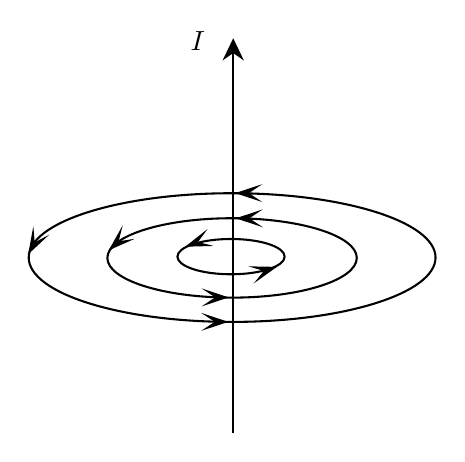
\begin{tikzpicture}[x=0.75pt,y=0.75pt,yscale=-1,xscale=1]
%uncomment if require: \path (0,440); %set diagram left start at 0, and has height of 440

%Straight Lines [id:da5191096557204329] 
\draw    (302.22,289.67) -- (302.22,102.67) ;
\draw [shift={(302.22,99.67)}, rotate = 450] [fill={rgb, 255:red, 0; green, 0; blue, 0 }  ][line width=0.08]  [draw opacity=0] (10.72,-5.15) -- (0,0) -- (10.72,5.15) -- (7.12,0) -- cycle    ;
%Shape: Ellipse [id:dp37246126193771323] 
\draw   (203.69,205.33) .. controls (203.69,188.21) and (247.56,174.33) .. (301.69,174.33) .. controls (355.81,174.33) and (399.69,188.21) .. (399.69,205.33) .. controls (399.69,222.45) and (355.81,236.33) .. (301.69,236.33) .. controls (247.56,236.33) and (203.69,222.45) .. (203.69,205.33) -- cycle ;
\draw  [fill={rgb, 255:red, 0; green, 0; blue, 0 }  ,fill opacity=1 ] (290.18,233.63) -- (298.25,236.3) -- (290.18,238.98) -- (294.22,236.3) -- cycle ;
%Shape: Ellipse [id:dp22619898713958686] 
\draw   (241.58,205.5) .. controls (241.58,194.94) and (268.48,186.38) .. (301.67,186.38) .. controls (334.85,186.38) and (361.75,194.94) .. (361.75,205.5) .. controls (361.75,216.06) and (334.85,224.63) .. (301.67,224.63) .. controls (268.48,224.63) and (241.58,216.06) .. (241.58,205.5) -- cycle ;
%Shape: Ellipse [id:dp7941660926092213] 
\draw   (275.33,204.88) .. controls (275.33,200.18) and (286.9,196.38) .. (301.17,196.38) .. controls (315.43,196.38) and (327,200.18) .. (327,204.88) .. controls (327,209.57) and (315.43,213.38) .. (301.17,213.38) .. controls (286.9,213.38) and (275.33,209.57) .. (275.33,204.88) -- cycle ;
\draw  [fill={rgb, 255:red, 0; green, 0; blue, 0 }  ,fill opacity=1 ] (290.39,221.85) -- (298.46,224.52) -- (290.39,227.2) -- (294.42,224.52) -- cycle ;
\draw  [fill={rgb, 255:red, 0; green, 0; blue, 0 }  ,fill opacity=1 ] (313.23,210.13) -- (321.73,210.29) -- (314.83,215.24) -- (317.88,211.49) -- cycle ;
\draw  [fill={rgb, 255:red, 0; green, 0; blue, 0 }  ,fill opacity=1 ] (313.13,189.08) -- (305.06,186.41) -- (313.13,183.73) -- (309.09,186.41) -- cycle ;
\draw  [fill={rgb, 255:red, 0; green, 0; blue, 0 }  ,fill opacity=1 ] (312.88,176.96) -- (304.81,174.28) -- (312.88,171.6) -- (308.84,174.28) -- cycle ;
\draw  [fill={rgb, 255:red, 0; green, 0; blue, 0 }  ,fill opacity=1 ] (289.06,199.33) -- (280.56,199.56) -- (287.23,194.29) -- (284.35,198.18) -- cycle ;
\draw  [fill={rgb, 255:red, 0; green, 0; blue, 0 }  ,fill opacity=1 ] (251.15,197.35) -- (243.38,200.81) -- (247.54,193.39) -- (246.36,198.09) -- cycle ;
\draw  [fill={rgb, 255:red, 0; green, 0; blue, 0 }  ,fill opacity=1 ] (210.43,196.55) -- (204.21,202.35) -- (205.73,193.99) -- (206.14,198.81) -- cycle ;

% Text Node
\draw (280.22,95.07) node [anchor=north west][inner sep=0.75pt]    {$I$};


\end{tikzpicture}
%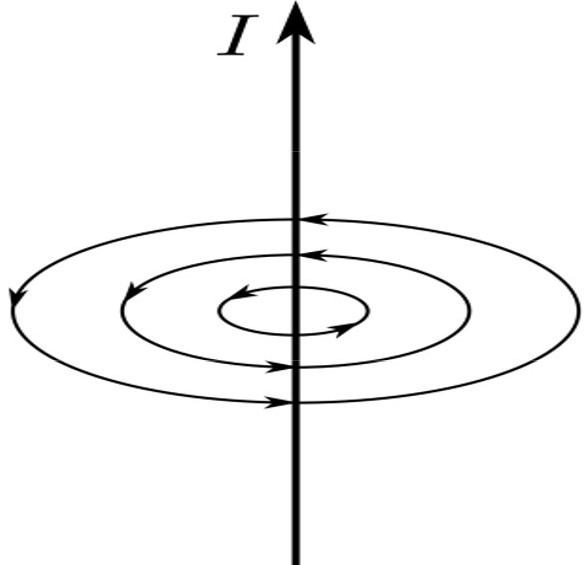
\includegraphics[scale=0.5]{Anh/Picture1 (2).jpg}
\end{center}
\item Ở gần vòng dây tròn có dòng điện chạy qua khép kín, từ trường giống như trong trường hợp dây thẳng. Khi ở xa, các đường sức từ tương ứng với đường sức từ của một lưỡng cực từ. Khu vực ở giữa có thể vẽ gần đúng như hình sau:
\begin{center}
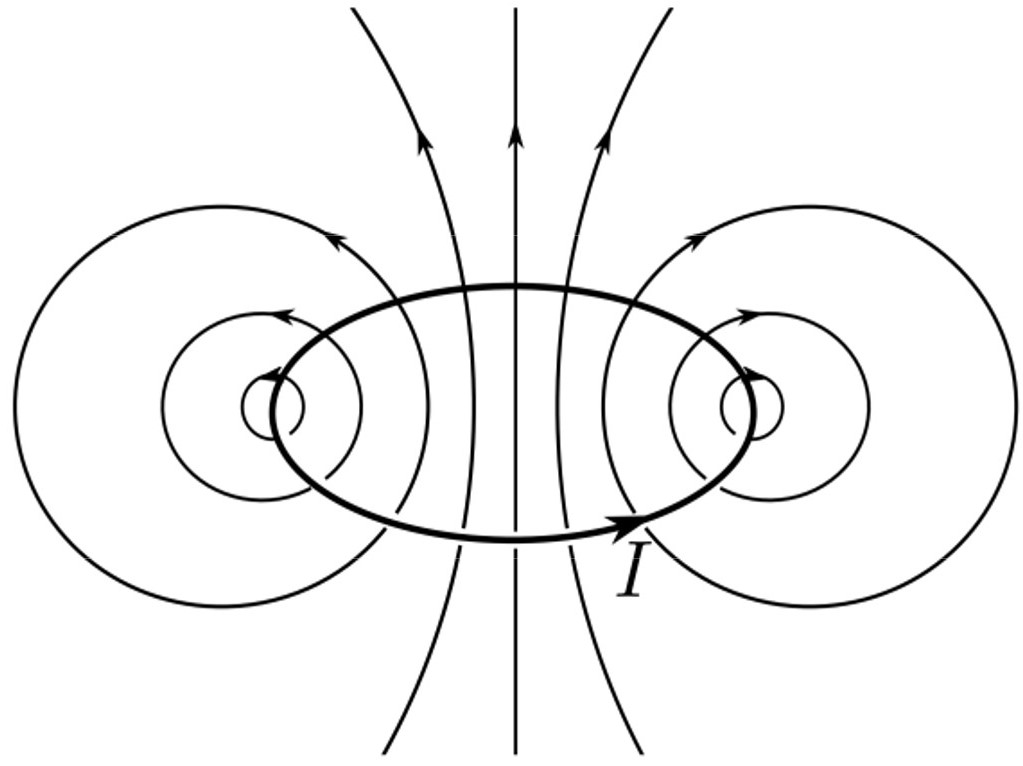
\includegraphics[scale=0.5]{Anh/Picture3 (2).jpg}
\end{center}
\item Nếu không có dây thẳng dài vô hạn, đường sức sẽ là các vòng tròn khép kín với bán kính nhỏ, quấn vòng quanh vòng dây điện tròn và kết thúc. Với sự xuất hiện của dây dài, một thành phần tiếp tuyến của từ trường được thêm vào, vì thế những đường sức từ tròn trước đó bắt đầu có khuynh hướng lệch theo phương tiếp tuyến xung quanh dây vô hạn trong khi đó vẫn quấn xung dày đặc xung quanh vòng dây tròn khép kín. Điều này tạo nên một mô hình xoắn dọc theo bề mặt của một hình phỏng xuyến được biểu diễn như hình sau.
\begin{center}
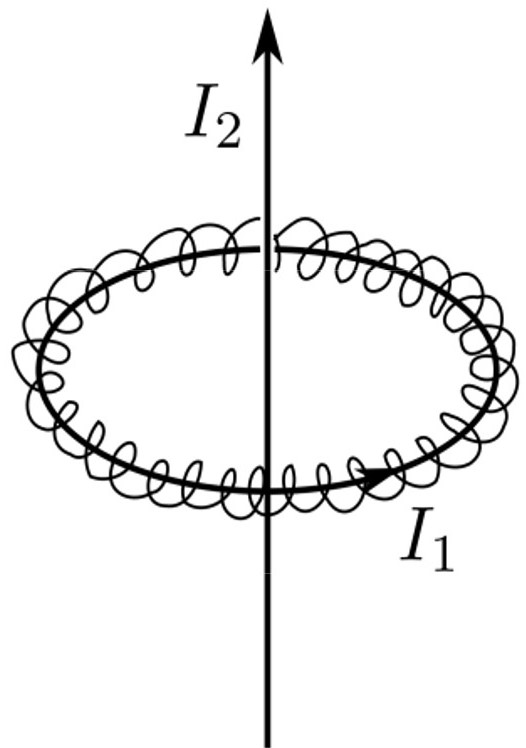
\includegraphics[scale=0.5]{Anh/Picture2 (2).jpg}
\end{center}
\item Sử dụng lập luận tương tự, khi không có sự hiện diện của vòng dây tròn khép kín, các đường sức từ cũng sẽ có hình dạng là những vòng tròn khép kín với bán kính nhỏ bao xung quanh dây dài vô hạn và rồi kết thúc. Nếu chúng ta cho thêm vòng dây điện tròn khép kín, các đường sức sẽ bắt đầu lệch ra khỏi những đường sức có dạng đường tròn khép kín ban đầu, những đường tròn khép kín ấy sẽ rất gần vị trí trung tâm và có bán kính cũng rất nhỏ (những đường sức nằm trên trục $z$ và trục $r$ trong hệ tọa độ trụ) trong khi quấn rất dày đặc xung quanh trục đối xứng (sau tất cả, cường độ từ trường từ dây dẫn thẳng dài vô hạn vẫn lớn hơn rất nhiều). Điều đó có nghĩa là các đường sức được hình thành có dạng một chuỗi xoắn dày đặc và từ từ rộng ra khi ngày càng ra xa mặt phẳng vòng dây điện tròn khép kín, cho đến khi nó khi trở về vô cùng (nơi mà cách rất xa so với vị trí của vòng dây điện tròn khép kín).
\begin{center}
    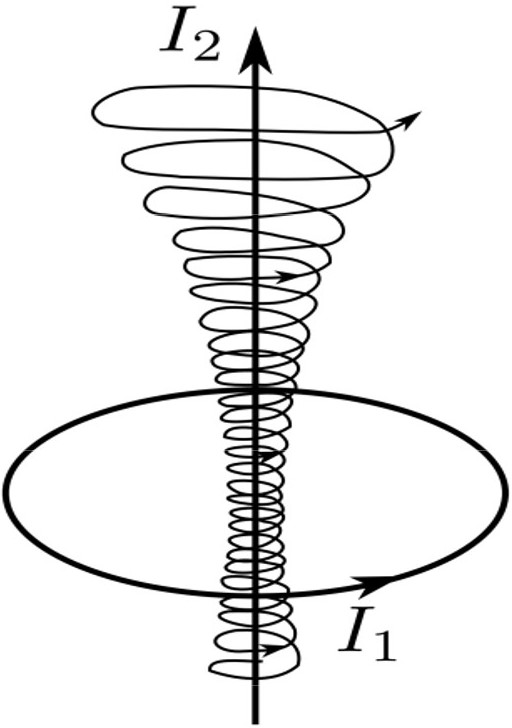
\includegraphics[scale=0.5]{Anh/Picture4 (2).jpg}
\end{center}
\end{enumerate}
    \item \textbf{Cold fusion:}\\
\begin{enumerate}[1)]
    \item 
Electron (muon) phải chịu tác dụng của lực tĩnh điện có độ lớn là:\[F=\dfrac{-1}{4\pi\varepsilon_0}\dfrac{2e^2}{R^2}. \tag{1} \label{1.1}\]
Số hai trong hệ thức là do trên thực tế, hạt nhân có điện tích là $+2e$. Đây là lực hút và đóng vai trò như một lực hướng tâm, chính vì thế, ta có: \[F=\dfrac{mv^2}{R}=\dfrac{p^2}{mR}.\tag{2} \label{1.2}\]
Từ (\ref{1.1}) và (\ref{1.2}), ta có được:
\[p=\sqrt{\dfrac{me^2}{2\pi \varepsilon_0 R}}.\]
Theo nguyên lí bất định, sai số tiêu chuẩn của động lượng và vị trí của hạt tuân theo bất đẳng thức sau:
\[\sigma_{x}\sigma_{p} \geq \dfrac{\hbar}{2} .\]
Với $\hbar=\dfrac{h}{2\pi}$ là hằng số Plank thu gọn. Vì chúng ta đang trong quá trình tính toán trên lí thuyết, sai số không phải là vấn đề lớn, vì thế, chúng ta có thể bỏ qua nó từ đây. Động lượng của electron (muon) luôn bằng $p$ vì thế $\sigma_{p}=p$, trong khi đó sai số tiêu chuẩn của vị trí luôn xấp xỉ bằng bán kính của đường tròn, vì thế $\sigma_{r}\sim R$.\\
Điều đó cho ta kết quả là:
\[\sqrt{\dfrac{me^2R}{\varepsilon_0}} \geq h.\]
Từ đó, ta giải ra $R$ xấp xỉ bằng:
\[R \sim \dfrac{h^2\varepsilon_0}{me^2}.\]
Đối với một electron, $R_{m=m_{e}}=1,7\times10^{-10}~\mathrm{m}$.\\
Đối với một muon, $R_{m=m_{\mu}}=8,1\times10^{-13}~\mathrm{m}$.
\item Do tính đối xứng, ta chỉ cần xét sự cân bằng lực ở một hạt nhân bởi vì hạt nhân còn lại cũng sẽ chịu sự tác dụng của những lực tương tự như vậy.\\
Sự cân bằng lực là sự cân bằng giữa các lực tĩnh điện giữa các hạt nhân với nhau và với các electron (đám mây muon). Biểu thức thứ nhất ta có được là biểu thức của lực đẩy:
\[F_1=\dfrac{1}{4\pi\varepsilon_0}\dfrac{e^2}{d^2}.\]
Đối với đám mây electron (muon), chỉ có những điện tích ở trong khối cầu có bán kính $d$ gây nên lực tĩnh điện. Điều đó có thể được xác định bằng cách sử dụng định luật Gauss cho khối cầu nói trên.\\
Điện tích bên trong khối cầu nhỏ hơn được xác định bởi $q=-2ed^3/8R^3$, bởi vì điện tích của khối cầu có phạm vi là lập phương bán kính.\\
Vì thế, lực của đám mây electron (muon) sẽ là:
\[F_2=-2e\dfrac{d^3}{8R^3}\dfrac{1}{4\pi\varepsilon_0}\dfrac{e}{d^2}.\]
Bởi vì có sự cân bằng lực, vì thế $F_1+F_2=0$, vì thế:
\[\dfrac{1}{4\pi\varepsilon_0}\dfrac{e^2}{d^2}-\dfrac{d^3}{4R^3}\dfrac{1}{4\pi\varepsilon_0}\dfrac{e^2}{d^2}=0.\]
Từ đó, ta tính được $d$ là:
\[d=R\sqrt[3]{4}.\]
\item Bởi vì $d$ phụ thuộc tuyến tính vào $R$ và $R$ tỉ lệ nghịch với khối lượng, khoảng cách giữa các hạt nhân sẽ được giảm bởi vì $m_{\mu}/m_{e}=207$.
\end{enumerate}
    \item \textbf{Inertial confinement fusion}
\begin{enumerate}[1)]
    \item Lớp vỏ chất lỏng là đồng chất và khối lượng phân bố đồng đều trên cả bề mặt và có thể biểu diễn bằng $\sigma=M/A$ với $A=4\pi r^2$ là tổng diện tích của lớp vỏ.\\
Do đó, khối lượng của một mẩu nhỏ là:
\[\Delta M=\sigma \Delta A=M.\dfrac{\Delta A}{4\pi r^2}.\]
    \item Vì áp suất bên ngoài lớn hơn rất nhiều so với áp suất bên trong, lớp vỏ sẽ bắt đầu co lại.\\
Tổng lực tác dụng lên một miếng nhỏ là $\Delta F=p_0\Delta A-p_{e}\Delta A\simeq-p_{e}\Delta A$, với chiều dương hệ quy chiếu là xuyên tâm và hướng ra ngoài.\\
Từ đó, gia tốc có biểu thức là:
\[a=\dfrac{\Delta F}{\Delta M}=\dfrac{-4\pi r^2p_{e}}{M}.\]
     \item Vì $p_{e}\gg p_0$, áp suất ở trạng thái cuối $p_{m}$ cũng sẽ rất nhỏ so với $p_{e}$. Quả thật là như thế, lớp vỏ sẽ co lại cho đến khi áp suất bên trong bằng áp suất bên ngoài $p_{e}$ và tiếp tục chuyển động do quán tính, cho đến khi áp suất bên trong cản trở hẳn chuyển động. Vì thế, thể tích ở trạng thái cuối sẽ rất nhỏ so với trậng thái ban đầu $-$ điều đó có thể suy ra từ những tính chất của quá trình đoạn nhiệt $V \sim  p^{-1/\gamma}$.\\
Vì thế, công của ngoại lực có thể tính bằng:
\[W=p_{e}\Delta V \approx p_e V_0.\]
Công này sẽ chuyển hóa thành nội năng,
\[W=c_{V}Nk_{B}T_{m},\]
Với $c_{V}=\dfrac{3}{2}k_{B}$ là nhiệt dung mol đẳng tích của hạt, và $N$ là tổng số hạt.\\
Bởi vì khí hoàn toàn bị ion hóa, nên mỗi phân tử DT sẽ tạo ra bốn hạt.\\
Vì thế, $N=4N_0$, với:
\[N_0=\dfrac{p_0V_0}{k_{B}T_0}.\]
Kết hợp tất cả những điều trên, ta thu được:
\[T_{m}=\dfrac{p_{e}}{4p_0}T_0.\]
Để tìm $r_{m}$, chúng ta kết hợp những tính chất của quá trình đoạn nhiệt và phương trình trạng thái khí lí tưởng thu được $V^{\gamma-1}T$ = hằng số. Điều đó cho ta $V \sim T^{-1/(\gamma-1)}$ và vì $r(V) \sim V^{1/3}$, ta có:
\[r_{m}=r\left(\dfrac{T_0}{T_{m}}\right)^{\frac{1}{3(\gamma-1)}}=r\left(\dfrac{4p_0}{p_{e}}\right)^{\frac{1}{3(\gamma-1)}}.\]
     \item Để tính được áp suất gây ra, chúng ta có thể nói rằng tất cả năng lượng của laser là dùng để tăng động năng của phần khối lượng đã bị bay hơi.\\
Gọi $M$ là khối lượng của phần vỏ ngoài đã bay hơi trong một đơn vị thời gian, xem xét trong một khoảng thời gian nhỏ là $\Delta t$, ta có định luật bảo toàn năng lượng là:
\[P\Delta t=\Delta M\dfrac{u^2}{2}=M\Delta t\dfrac{u^2}{2}.\]
Do đó,
\[M=\dfrac{2P}{u^2}.\]
Từ định luật bảo toàn động lượng, chúng ta có thể viết:
\[4\pi r^2 p_{e}=Mu,\]
do đó:
\[p_{e}=\dfrac{Mu}{4\pi r^2}=\dfrac{2P}{4\pi r^2u}.\]
\end{enumerate}
\end{enumerate}
\end{loigiai}


\begin{vd}[Động cơ đồng cực]
  Một động cơ đồng cực là động cơ gồm một khung dây cho dòng điện không đổi $I$ chạy qua được đặt trong vùng từ trường tĩnh. Khung dây có thể quay tự do quanh một trục cố định sao cho góc tạo bởi dòng điện và từ trường là không đổi ở mọi phần của khung dây. Do đó lực điện từ tác dụng lên khung dây là liên tục và không cần công tắc để đổi chiều dòng điện sau mỗi nửa chu kì như một số loại động cơ khác. Tuy nhiên nó vẫn cần một vòng trượt hoặc một chổi than tiếp xúc để có thể hoạt động. “Đồng cực” có nghĩa là hướng phân cực của khung dây (chiều dòng điện của mọi điểm trên dây dẫn) và từ trường hợp với nhau một góc không đổi theo thời gian và không cần công tắc đảo chiều dòng. Một mô hình đơn giản của loại động cơ này được mô tả như hình vẽ, tham khảo từ Wikipedia.
  \begin{center}
\tikzset{every picture/.style={line width=0.75pt}} %set default line width to 0.75pt        

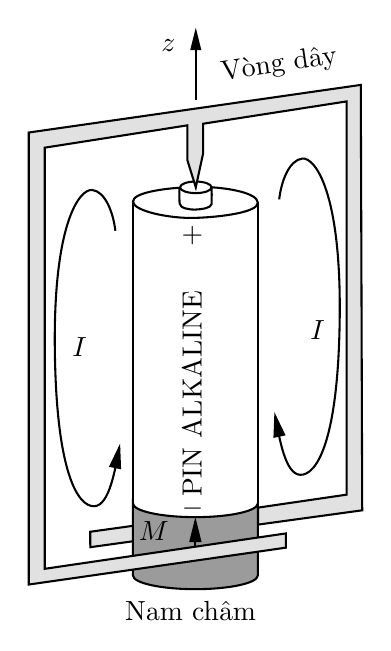
\begin{tikzpicture}[x=0.75pt,y=0.75pt,yscale=-1,xscale=1]
%uncomment if require: \path (0,300); %set diagram left start at 0, and has height of 300

%Shape: Parallelogram [id:dp9905349717591636] 
\draw  [fill={rgb, 255:red, 225; green, 225; blue, 225 }  ,fill opacity=1 ] (290.33,245.66) -- (329.82,240.18) -- (329.86,247.62) -- (290.37,253.09) -- cycle ;
%Curve Lines [id:da5688680161114963] 
\draw [line width=0.75]    (348.78,79.72) .. controls (356.99,80.14) and (370.87,82.45) .. (371.08,87.08) .. controls (371.29,91.71) and (353.62,94.02) .. (341,94.44) .. controls (328.38,94.86) and (311.13,91.08) .. (310.92,86.66) .. controls (310.71,82.24) and (326.28,80.35) .. (333.22,79.93) ;
%Curve Lines [id:da9603174449394891] 
\draw    (333.22,79.93) .. controls (333.38,81.18) and (333.25,85.04) .. (333.38,87.49) .. controls (333.63,89.89) and (338.3,90.55) .. (341.2,90.42) .. controls (344.36,90.32) and (348.4,89.66) .. (348.77,87.87) .. controls (348.9,84.11) and (348.9,81.97) .. (348.78,79.72) ;
%Shape: Ellipse [id:dp21468822030138313] 
\draw   (333.6,79.72) .. controls (333.6,78.18) and (337,76.93) .. (341.19,76.93) .. controls (345.39,76.93) and (348.78,78.18) .. (348.78,79.72) .. controls (348.78,81.26) and (345.39,82.5) .. (341.19,82.5) .. controls (337,82.5) and (333.6,81.26) .. (333.6,79.72) -- cycle ;
%Straight Lines [id:da7062712274141836] 
\draw    (371.08,87.08) -- (371.08,236.6) ;
%Straight Lines [id:da028657021666151916] 
\draw    (310.92,87.08) -- (310.92,236.6) ;
%Flowchart: Stored Data [id:dp8777673631796328] 
\draw  [fill={rgb, 255:red, 155; green, 155; blue, 155 }  ,fill opacity=1 ] (310.92,266.71) -- (310.92,232.01) .. controls (310.92,235.66) and (324.39,238.62) .. (341,238.62) .. controls (357.61,238.62) and (371.08,235.66) .. (371.08,232.01) -- (371.08,266.71) .. controls (371.08,270.36) and (357.61,273.32) .. (341,273.32) .. controls (324.39,273.32) and (310.92,270.36) .. (310.92,266.71) -- cycle ;
%Straight Lines [id:da7748569407235104] 
\draw    (341.18,37.83) -- (341.18,4.85) ;
\draw [shift={(341.18,2.85)}, rotate = 450] [fill={rgb, 255:red, 0; green, 0; blue, 0 }  ][line width=0.08]  [draw opacity=0] (10.8,-2.7) -- (0,0) -- (10.8,2.7) -- cycle    ;
%Shape: Polygon [id:ds8295801816113073] 
\draw  [fill={rgb, 255:red, 225; green, 225; blue, 225 }  ,fill opacity=1 ] (260.7,53.31) -- (260.7,271.1) -- (384.56,253.33) -- (384.56,246.47) -- (268.42,263.51) -- (268.42,60.61) -- (337.1,49.86) -- (337.1,66.51) -- (341.19,79.72) -- (344.7,63.49) -- (344.7,49.08) -- (413.84,38.33) -- (413.84,227.79) -- (371.24,234.02) -- (371.24,242.21) -- (421.38,235.33) -- (420.69,30.37) -- cycle ;
%Curve Lines [id:da941413031429216] 
\draw    (304.33,205.19) .. controls (302.4,215.23) and (299.63,233.12) .. (292.27,233.36) .. controls (284.41,233.63) and (273.92,217.31) .. (273.27,157.34) .. controls (272.61,97.38) and (285.06,80.34) .. (291.29,80.99) .. controls (297.52,81.65) and (301.45,91.81) .. (302.43,100.65) ;
\draw [shift={(304.72,203.22)}, rotate = 101.77] [fill={rgb, 255:red, 0; green, 0; blue, 0 }  ][line width=0.08]  [draw opacity=0] (12,-3) -- (0,0) -- (12,3) -- cycle    ;
%Shape: Boxed Bezier Curve [id:dp9967219654755937] 
\draw    (379.48,190.05) .. controls (381.41,200.09) and (384.18,217.98) .. (391.53,218.23) .. controls (399.4,218.49) and (409.88,202.17) .. (410.54,142.2) .. controls (411.2,82.24) and (398.74,65.2) .. (392.52,65.85) .. controls (386.29,66.51) and (382.36,76.67) .. (381.38,85.51) ;
\draw [shift={(379.08,188.08)}, rotate = 78.23] [fill={rgb, 255:red, 0; green, 0; blue, 0 }  ][line width=0.08]  [draw opacity=0] (12,-3) -- (0,0) -- (12,3) -- cycle    ;
%Straight Lines [id:da0001273221005622105] 
\draw    (341,252.64) -- (341,240.62) ;
\draw [shift={(341,238.62)}, rotate = 450] [fill={rgb, 255:red, 0; green, 0; blue, 0 }  ][line width=0.08]  [draw opacity=0] (12,-3) -- (0,0) -- (12,3) -- cycle    ;

% Text Node
\draw (350.94,17.65) node [anchor=north west][inner sep=0.75pt]  [rotate=-351.63] [align=left] {Vòng dây};
% Text Node
\draw (305.7,277.65) node [anchor=north west][inner sep=0.75pt]   [align=left] {Nam châm};
% Text Node
\draw (333.44,230.34) node [anchor=north west][inner sep=0.75pt]  [rotate=-270] [align=left] {PIN ALKALINE};
% Text Node
\draw (280.24,150.73) node [anchor=north west][inner sep=0.75pt]    {$I$};
% Text Node
\draw (394.93,142.21) node [anchor=north west][inner sep=0.75pt]    {$I$};
% Text Node
\draw (332.95,228.57) node [anchor=north west][inner sep=0.75pt]    {$-$};
% Text Node
\draw (332.9,97.09) node [anchor=north west][inner sep=0.75pt]    {$+$};
% Text Node
\draw (323.13,7) node [anchor=north west][inner sep=0.75pt]    {$z$};
% Text Node
\draw (312.25,239.25) node [anchor=north west][inner sep=0.75pt]    {$M$};


\end{tikzpicture}

  \end{center}
  
Nguyên lí hoạt động của động cơ như sau: Một nguồn pin tải dòng điện cố định đi qua khung dây kép như hình vẽ, hệ đặt trong từ trường cố định tạo ra bởi một nam châm vĩnh cửu hình trụ được đặt bên dưới nguồn pin, tiếp xúc với cực âm của nguồn (xem hình vẽ). Từ trường do đó là đối xứng quanh trục $z$ và có độ lớn không đổi theo thời gian và khung dây có thể quay tự do quanh trục $z$ cố định.\\
    \begin{center}
     

\tikzset{every picture/.style={line width=0.75pt}} %set default line width to 0.75pt        

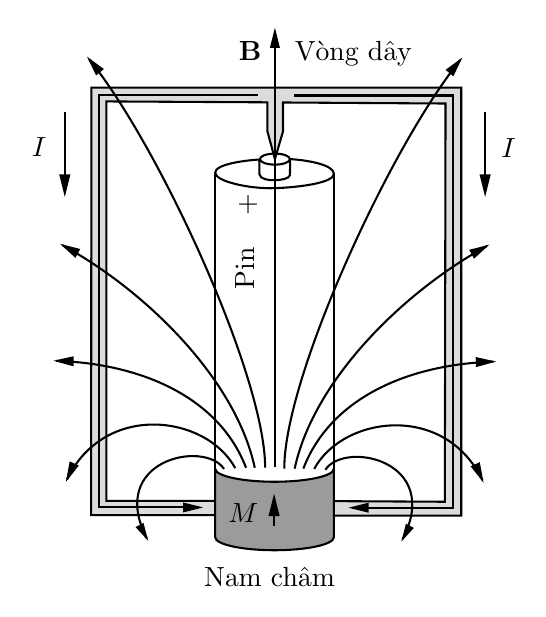
\begin{tikzpicture}[x=0.75pt,y=0.75pt,yscale=-0.9,xscale=0.9]
%uncomment if require: \path (0,336); %set diagram left start at 0, and has height of 336

%Shape: Polygon [id:ds5398321534883261] 
\draw  [fill={rgb, 255:red, 220; green, 220; blue, 220 }  ,fill opacity=1 ] (430.23,47.56) -- (430.23,276.71) -- (360.82,276.71) -- (360.82,268.92) -- (421.43,269.26) -- (421.8,56.07) -- (334.8,55.52) -- (334.8,71.02) -- (330.47,85.83) -- (326.47,71.03) -- (326.47,55.43) -- (240.23,54.95) -- (240.23,268.79) -- (298.87,268.79) -- (298.87,276.39) -- (232.07,276.39) -- (232.23,47.56) -- cycle ;
%Curve Lines [id:da7652155646336201] 
\draw [line width=0.75]    (338.49,85.83) .. controls (347.16,86.28) and (361.82,88.72) .. (362.04,93.61) .. controls (362.27,98.5) and (343.6,100.94) .. (330.27,101.39) .. controls (316.93,101.83) and (298.71,97.83) .. (298.49,93.17) .. controls (298.27,88.5) and (314.71,86.5) .. (322.04,86.06) ;
%Curve Lines [id:da8263889077812194] 
\draw    (322.04,86.06) .. controls (322.21,87.38) and (322.08,91.46) .. (322.21,94.05) .. controls (322.48,96.58) and (327.41,97.27) .. (330.48,97.14) .. controls (333.81,97.03) and (338.08,96.34) .. (338.48,94.45) .. controls (338.61,90.47) and (338.61,88.21) .. (338.49,85.83) ;
%Shape: Ellipse [id:dp8997122003794547] 
\draw   (322.45,85.83) .. controls (322.45,84.21) and (326.04,82.89) .. (330.47,82.89) .. controls (334.9,82.89) and (338.49,84.21) .. (338.49,85.83) .. controls (338.49,87.46) and (334.9,88.78) .. (330.47,88.78) .. controls (326.04,88.78) and (322.45,87.46) .. (322.45,85.83) -- cycle ;
%Straight Lines [id:da585831478304778] 
\draw    (362.04,93.61) -- (362.04,251.57) ;
%Straight Lines [id:da16307441614756546] 
\draw    (298.49,93.61) -- (298.49,251.57) ;
%Flowchart: Stored Data [id:dp3009048631910518] 
\draw  [fill={rgb, 255:red, 155; green, 155; blue, 155 }  ,fill opacity=1 ] (298.49,288.23) -- (298.49,251.57) .. controls (298.49,255.42) and (312.72,258.55) .. (330.27,258.55) .. controls (347.82,258.55) and (362.04,255.42) .. (362.04,251.57) -- (362.04,288.23) .. controls (362.04,292.08) and (347.82,295.21) .. (330.27,295.21) .. controls (312.72,295.21) and (298.49,292.08) .. (298.49,288.23) -- cycle ;
%Straight Lines [id:da3184761056631049] 
\draw    (330.02,282.39) -- (330.02,266.99) ;
\draw [shift={(330.02,264.99)}, rotate = 450] [fill={rgb, 255:red, 0; green, 0; blue, 0 }  ][line width=0.08]  [draw opacity=0] (12,-3) -- (0,0) -- (12,3) -- cycle    ;
%Curve Lines [id:da5942792400252743] 
\draw    (303.24,251.7) .. controls (292.68,235.86) and (240.31,246.9) .. (261.9,288.86) ;
\draw [shift={(262.58,290.14)}, rotate = 241.53] [fill={rgb, 255:red, 0; green, 0; blue, 0 }  ][line width=0.08]  [draw opacity=0] (9.6,-2.4) -- (0,0) -- (9.6,2.4) -- cycle    ;
%Curve Lines [id:da4513780347454881] 
\draw    (309.24,251.26) .. controls (293.62,222.66) and (239.24,215.62) .. (219.18,257.31) ;
\draw [shift={(218.58,258.59)}, rotate = 294.4] [fill={rgb, 255:red, 0; green, 0; blue, 0 }  ][line width=0.08]  [draw opacity=0] (10.8,-2.7) -- (0,0) -- (10.8,2.7) -- cycle    ;
%Curve Lines [id:da8833941265643703] 
\draw    (315.02,251.08) .. controls (300.72,213.72) and (259.63,195.31) .. (213.32,193.83) ;
\draw [shift={(211.91,193.79)}, rotate = 361.40999999999997] [fill={rgb, 255:red, 0; green, 0; blue, 0 }  ][line width=0.08]  [draw opacity=0] (10.8,-2.7) -- (0,0) -- (10.8,2.7) -- cycle    ;
%Curve Lines [id:da4276881203243461] 
\draw    (319.69,251.08) .. controls (309.57,203.82) and (261.77,156.61) .. (216.83,131.95) ;
\draw [shift={(215.47,131.21)}, rotate = 388.33000000000004] [fill={rgb, 255:red, 0; green, 0; blue, 0 }  ][line width=0.08]  [draw opacity=0] (10.8,-2.7) -- (0,0) -- (10.8,2.7) -- cycle    ;
%Curve Lines [id:da6935502583331479] 
\draw    (325.24,251.03) .. controls (325.24,201.93) and (268.18,78.12) .. (231.03,32.39) ;
\draw [shift={(229.91,31.03)}, rotate = 410.22] [fill={rgb, 255:red, 0; green, 0; blue, 0 }  ][line width=0.08]  [draw opacity=0] (10.8,-2.7) -- (0,0) -- (10.8,2.7) -- cycle    ;

%Curve Lines [id:da10521949349921678] 
\draw    (357.48,252.13) .. controls (368.04,236.29) and (420.42,247.33) .. (398.83,289.29) ;
\draw [shift={(398.15,290.57)}, rotate = 298.47] [fill={rgb, 255:red, 0; green, 0; blue, 0 }  ][line width=0.08]  [draw opacity=0] (9.6,-2.4) -- (0,0) -- (9.6,2.4) -- cycle    ;
%Curve Lines [id:da6475337590116637] 
\draw    (351.48,251.68) .. controls (367.1,223.08) and (421.49,216.05) .. (441.55,257.74) ;
\draw [shift={(442.15,259.02)}, rotate = 245.6] [fill={rgb, 255:red, 0; green, 0; blue, 0 }  ][line width=0.08]  [draw opacity=0] (10.8,-2.7) -- (0,0) -- (10.8,2.7) -- cycle    ;
%Curve Lines [id:da8795814952017094] 
\draw    (345.7,251.51) .. controls (360,214.15) and (401.09,195.74) .. (447.41,194.26) ;
\draw [shift={(448.82,194.22)}, rotate = 538.5899999999999] [fill={rgb, 255:red, 0; green, 0; blue, 0 }  ][line width=0.08]  [draw opacity=0] (10.8,-2.7) -- (0,0) -- (10.8,2.7) -- cycle    ;
%Curve Lines [id:da5266593407059388] 
\draw    (341.04,251.51) .. controls (351.16,204.25) and (398.96,157.04) .. (443.9,132.38) ;
\draw [shift={(445.26,131.64)}, rotate = 511.67] [fill={rgb, 255:red, 0; green, 0; blue, 0 }  ][line width=0.08]  [draw opacity=0] (10.8,-2.7) -- (0,0) -- (10.8,2.7) -- cycle    ;
%Curve Lines [id:da686496351033266] 
\draw    (335.48,251.46) .. controls (335.48,202.36) and (392.55,78.55) .. (429.7,32.82) ;
\draw [shift={(430.82,31.46)}, rotate = 489.78] [fill={rgb, 255:red, 0; green, 0; blue, 0 }  ][line width=0.08]  [draw opacity=0] (10.8,-2.7) -- (0,0) -- (10.8,2.7) -- cycle    ;

%Straight Lines [id:da5418277081629266] 
\draw    (330.46,250.9) -- (330.46,17.53) ;
\draw [shift={(330.46,15.53)}, rotate = 450] [fill={rgb, 255:red, 0; green, 0; blue, 0 }  ][line width=0.08]  [draw opacity=0] (10.8,-2.7) -- (0,0) -- (10.8,2.7) -- cycle    ;
%Curve Lines [id:da009594011998967478] 
\draw     ;
%Straight Lines [id:da97513275658264] 
\draw    (321.4,51.63) -- (236.07,51.63) -- (236.07,272.3) -- (290.07,272.3) ;
\draw [shift={(292.07,272.3)}, rotate = 180] [fill={rgb, 255:red, 0; green, 0; blue, 0 }  ][line width=0.08]  [draw opacity=0] (10.8,-2.7) -- (0,0) -- (10.8,2.7) -- cycle    ;
%Shape: Boxed Line [id:dp10260437502204112] 
\draw    (340.48,51.78) -- (425.81,51.78) -- (425.81,272.45) -- (371.81,272.45) ;
\draw [shift={(369.81,272.45)}, rotate = 360] [fill={rgb, 255:red, 0; green, 0; blue, 0 }  ][line width=0.08]  [draw opacity=0] (10.8,-2.7) -- (0,0) -- (10.8,2.7) -- cycle    ;
%Straight Lines [id:da46982581709923377] 
\draw    (218,60.37) -- (218,104.03) ;
\draw [shift={(218,106.03)}, rotate = 270] [fill={rgb, 255:red, 0; green, 0; blue, 0 }  ][line width=0.08]  [draw opacity=0] (12,-3) -- (0,0) -- (12,3) -- cycle    ;
%Straight Lines [id:da03595452532800336] 
\draw    (443,60.37) -- (443,104.03) ;
\draw [shift={(443,106.03)}, rotate = 270] [fill={rgb, 255:red, 0; green, 0; blue, 0 }  ][line width=0.08]  [draw opacity=0] (12,-3) -- (0,0) -- (12,3) -- cycle    ;


% Text Node
\draw (303.91,268.68) node [anchor=north west][inner sep=0.75pt]    {$M$};
% Text Node
\draw (290.91,302.83) node [anchor=north west][inner sep=0.75pt]   [align=left] {Nam châm};
% Text Node
\draw (198.67,72.77) node [anchor=north west][inner sep=0.75pt]    {$I$};
% Text Node
\draw (450,73.43) node [anchor=north west][inner sep=0.75pt]    {$I$};
% Text Node
\draw (307.5,157.2) node [anchor=north west][inner sep=0.75pt]  [rotate=-270] [align=left] {Pin};
% Text Node
\draw (308.67,103.77) node [anchor=north west][inner sep=0.75pt]    {$+$};
% Text Node
\draw (309.5,21.4) node [anchor=north west][inner sep=0.75pt]    {$\mathbf{B}$};
% Text Node
\draw (339.5,21) node [anchor=north west][inner sep=0.75pt]   [align=left] {Vòng dây};


\end{tikzpicture}

    \end{center}
Các thông số chiều dài, khối lượng và điện trở khung dây (và của pin, nam châm), hiệu điện thế của pin và từ trường của nam châm ở mọi điểm trong không gian được giả sử như đã biết. Tìm moment ngẫu lực tác dụng lên khung dây và vận tốc góc của khung như một hàm của thời gian $t$.

\end{vd}
\begin{loigiai}
Motor của chúng ta được mô hình hóa như trên biểu đồ (xem hình vẽ), hình vẽ chỉ thể hiện một nửa khung dây vì bài toán có tính đối xứng. Chúng ta sử dụng hệ tọa độ trụ $(r, \phi, z)$ với gốc tọa độ $O$ nằm ở trọng tâm của nam châm hình trụ, có bán kính $b$ và chiều dài $l$. Trục $z$ đồng trục với trục của nam châm và trục của pin, ở đây pin được mô hình như một nguồn điện có hiệu điện thế $V$. Mạch điện $ACDEF$ được khép kín bằng tiếp xúc chổi than (mũi tên màu trắng trên hình vẽ) với nam châm tại điểm $A \equiv (0,\phi,l/2)$ và $F \equiv (b, \phi, 0)$ do đó dòng điện có thể chạy qua nam châm dẫn điện. Mạch điện có thể quay tự do quanh trục $z$. Đặt $a (>b)$ và $h$ lần lượt là kích thước của khung dây theo phương ngang và phương dọc.
 \begin{center}
     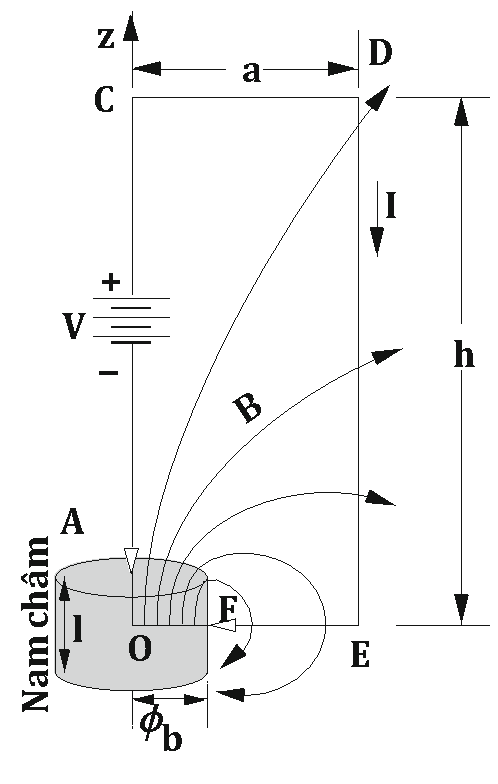
\includegraphics[scale=0.6]{Anh/Nam_P3.pdf}
 \end{center}
Ta đặt $\ot{B} = \ot{B} (r, \phi, z)$ là từ trường tạo ra bởi nam châm, không phụ thuộc vào $\phi$ và có $B_{\phi} \equiv 0$. Một vài đường sức từ của $\ot{B}$ được vẽ trên hình. Từ trường tại mặt phẳng $z=0$ song song với trục $z$, hướng thẳng đứng lên trên với $r<b$ và hướng xuống dưới đối với $r>b$. Để đơn giản hóa bài toán chúng ta giả sử $\ot{B} (r,\phi, 0) = B_0 \hat{{z}} $ đối với $r<b$, với $B_0$ không phụ thuộc vào $r$, dù xấp xỉ này chỉ đúng khi $l \gg b$.
 \begin{center}
     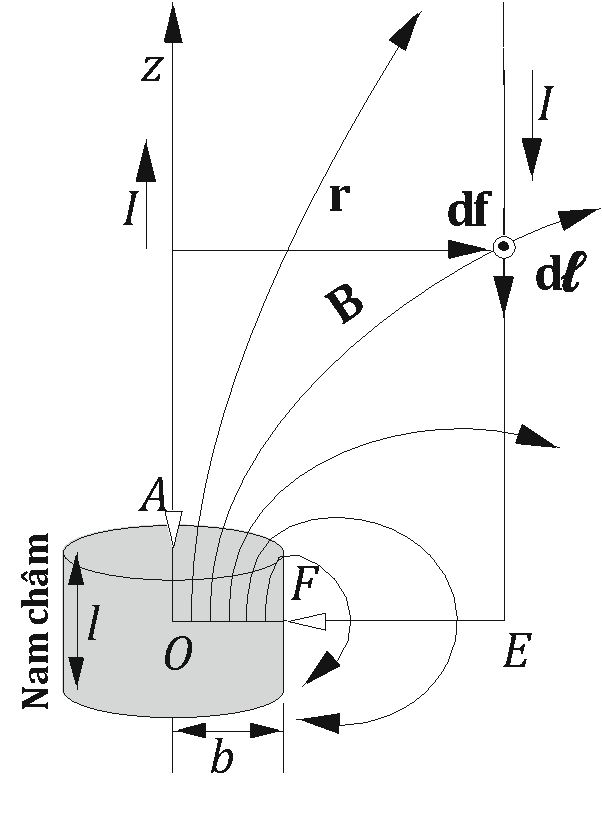
\includegraphics[scale=0.6]{Anh/Nam_P4.pdf}
 \end{center}
Nguồn điện sẽ đẩy một dòng điện $I$ đi qua mạch điện. Khi khung dây không quay, ta dễ dàng có $I= V/R$ nhưng khi khung dây quay, chúng ta phải tính đến hiệu ứng của khung dây chuyển động trong từ trường. Vì từ trường $\ot{B}$ nằm trong mặt phẳng khung dây nên lực $\dd\ot{f} = I \dd\ot{l}\times \ot{B}$ tác dụng lên một vi phân chiều dài $\dd\ot{l}$ của khung dây là vuông góc với mặt phẳng vòng dây (hoặc là mặt giấy đối với hình vẽ). Moment tương ứng đối với trục $z$ của lực là 
        \[ \dd \ot{\tau}= \ot{r} \times \dd \ot{f} = b_m I \ot{r} \times (\dd \ot{l} \times \ot{B}),  \tag{1}\label{n.1}\]
với $\ot{r}$ là khoảng cách của vi phân độ dài $\dd\ot{l}$ đến trục $z$. Phương của vi phân moment lực $\dd \ot{\tau}$ luôn song song với ${\hat{z}}$, không phụ thuộc vào vị trí của $\dd\ot{l}$ mà chúng ta xét. Đối với tích vector $\dd\ot{l} \times\ot{B}$ ta có
      \[\dd\ot{l}\times \ot{B}=-\hat{{\phi}}B \dd l \sin\theta = - \hat{{\phi}} B \dd l \cos \psi\]
            \[=-\hat{{\phi}}\ot{B} \cdot \hat{n} \dd l, \tag{2}\]

với $\theta$ là góc hợp bởi $\dd \ot{l}$ và $\ot{B}$, ${\hat{n}}$ là vector đơn vị vuông góc với $\dd\ot{l}$, và $\psi = \theta - \pi/2$ là góc hợp giữa $\ot{B}$ và ${\hat{n}}$ (xem hình vẽ). 
  \begin{center}


\tikzset{every picture/.style={line width=0.75pt}} %set default line width to 0.75pt        

\begin{tikzpicture}[x=0.75pt,y=0.75pt,yscale=-1,xscale=1]
%uncomment if require: \path (0,300); %set diagram left start at 0, and has height of 300

%Straight Lines [id:da4574314470092409] 
\draw    (252.31,144.28) -- (313.6,83) -- (374.47,22.12) ;
\draw [shift={(376.59,20)}, rotate = 495] [fill={rgb, 255:red, 0; green, 0; blue, 0 }  ][line width=0.08]  [draw opacity=0] (10.72,-5.15) -- (0,0) -- (10.72,5.15) -- (7.12,0) -- cycle    ;
%Straight Lines [id:da43449029535351946] 
\draw    (252.31,144.28) -- (408.6,144.28) ;
\draw [shift={(411.6,144.28)}, rotate = 180] [fill={rgb, 255:red, 0; green, 0; blue, 0 }  ][line width=0.08]  [draw opacity=0] (10.72,-5.15) -- (0,0) -- (10.72,5.15) -- (7.12,0) -- cycle    ;
%Straight Lines [id:da7839461358085928] 
\draw    (252.31,144.28) -- (252.31,269.42) ;
\draw [shift={(252.31,272.42)}, rotate = 270] [fill={rgb, 255:red, 0; green, 0; blue, 0 }  ][line width=0.08]  [draw opacity=0] (10.72,-5.15) -- (0,0) -- (10.72,5.15) -- (7.12,0) -- cycle    ;
%Shape: Arc [id:dp1604699560533387] 
\draw  [draw opacity=0][dash pattern={on 4.5pt off 4.5pt}] (301.95,96.63) .. controls (315.87,111.15) and (323.33,131.62) .. (320.54,153.12) .. controls (316.05,187.84) and (286.41,213.14) .. (252.31,213.09) -- (252.31,144.28) -- cycle ; \draw  [dash pattern={on 4.5pt off 4.5pt}] (301.95,96.63) .. controls (315.87,111.15) and (323.33,131.62) .. (320.54,153.12) .. controls (316.05,187.84) and (286.41,213.14) .. (252.31,213.09) ;
%Shape: Arc [id:dp08212124771975149] 
\draw  [draw opacity=0][dash pattern={on 4.5pt off 4.5pt}] (292.89,143.68) .. controls (292.92,145.6) and (292.81,147.54) .. (292.56,149.5) .. controls (289.9,169.97) and (272.42,184.9) .. (252.31,184.87) -- (252.31,144.28) -- cycle ; \draw  [dash pattern={on 4.5pt off 4.5pt}] (292.89,143.68) .. controls (292.92,145.6) and (292.81,147.54) .. (292.56,149.5) .. controls (289.9,169.97) and (272.42,184.9) .. (252.31,184.87) ;
%Shape: Arc [id:dp537421311028123] 
\draw  [draw opacity=0][dash pattern={on 4.5pt off 4.5pt}] (320.32,78.57) .. controls (336.32,95.26) and (346.29,117.5) .. (347.36,141.56) -- (250.08,146) -- cycle ; \draw  [dash pattern={on 4.5pt off 4.5pt}] (320.32,78.57) .. controls (336.32,95.26) and (346.29,117.5) .. (347.36,141.56) ;


% Text Node
\draw (228,192.4) node [anchor=north west][inner sep=0.75pt]    {$\dd \ot{\ell}$};
% Text Node
\draw (303.32,59.38) node [anchor=north west][inner sep=0.75pt]  [rotate=-314.09]  {$\ot{B}$};
% Text Node
\draw (283.8,160.4) node [anchor=north west][inner sep=0.75pt]    {$\dfrac{\pi }{2}$};
% Text Node
\draw (384.8,146.4) node [anchor=north west][inner sep=0.75pt]    {$\ot{\hat{n}}$};
% Text Node
\draw (346.8,92.4) node [anchor=north west][inner sep=0.75pt]    {$\psi $};
% Text Node
\draw (307.8,189.4) node [anchor=north west][inner sep=0.75pt]    {$\theta $};


\end{tikzpicture}
\end{center}
Vì ${\hat{r}}$ là vuông góc với $\hat{\boldsymbol{\phi}}$ (vector đơn vị của hai tọa độ độc lập), chúng ta có tổng moment tác dụng lên khung dây 
  \[ \tau = b_m I \int_{A}^{F} \ot{r} \times ( \dd \ot{l} \times \ot{B}) = - \hat{{z}} b_m I \int_{A}^{F} \ot{B} \cdot \hat{n} r\,\dd l. \tag{3} \]

Biểu thức cuối của phương trình trên có thể tính được tích phân mà không cần gần đúng nếu chúng ta chứng minh được tích phân đường của $\ot{B} \cdot \hat{n} r $ quanh vòng kín $OCDEO$ (xem hình vẽ) là bằng không, đó là
  \[\oint\ot{B} \cdot \hat{n} r \,\dd l = \int_{A}^{F} \ot{B}\cdot\hat{n} r \,\dd l + \int_{F}^{O} \ot{B}\cdot \hat{n} r  \,\dd l + \int_{O}^{A} \ot{B}\cdot \hat{n} r \, \dd l =0. \tag {4}\]
Đầu tiên, chúng ta để ý rằng tích phân này dọc trên đoạn $\overline{OC}$ là bằng không, bởi vì $r$ bằng không và hơn nữa là do $\ot{B}$ song song với $\dd\ot{l}$. Do đó tích phân trên thu gọn lại thành
  \[ \begin{aligned}
       \oint \ot{B}\cdot \hat{n} r \, \dd l &= \int_{C}^{D} \ot{B} \cdot \hat{n} r \, \dd r - \int_{D}^{E} \ot{B} \cdot \hat{n} r \, \dd z - \int_{E}^{O} \ot{B} \cdot \hat{n} r \, \dd r\\
         &= \int_{C}^{D} \ot{B} \cdot \hat{n} r \, \dd r + \int_{E}^{D} \ot{B} \cdot \hat{n} r \, \dd z + \int_{O}^{E} \ot{B}\cdot \hat{n} r \, \dd r,  \end{aligned} \tag{5}\]

vì $\dd l= \dd r$ dọc theo $\overline{CD}$, $\dd l=-\dd z$ dọc theo $\overline{DE}$ và $\dd l = -\dd r$ dọc theo $\overline{EO}$.\\
 Ở bước tiếp theo, chúng ta tạo ra hình trụ bằng cách quay khung dây quanh trục $z$ (xem hình vẽ).
 \begin{center}
     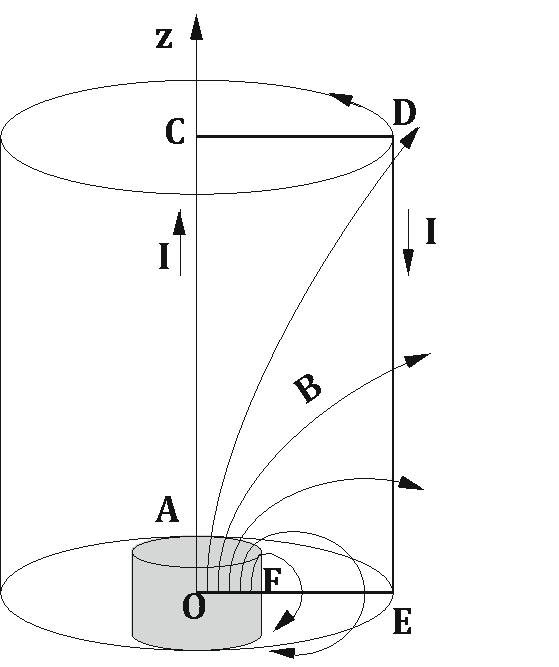
\includegraphics[scale=0.6]{Anh/Nam_P5.pdf}
 \end{center}
 Phần từ thông của từ trường $\ot{B}$ đi qua toàn bộ diện tích hình trụ là 
  \[\int_{\text{trên}} \ot{B} \cdot \hat{n} \, \dd S + \int_\text{{bên}} \ot{B} \cdot \hat{n} \, \dd S+ \int_\text{{dưới}} \ot{B} \cdot \hat{n} \, \dd S =0, \tag{6}\]
vì $\nabla\cdot\ot{B}=0$ nên phương trình $6)$ có thể viết lại thành
   \[ \begin{aligned} 0 &= \int_{0}^{a} \ot{B} (r,\phi,h) \cdot {\hat{n}} 2\pi r \, \dd r + \int_{0}^{h} \ot{B} (a, \phi, z) \cdot {\hat{n}} 2 \pi e \, \dd z\\
    &+ \int_{0}^{a} \ot{B} (r,\phi,0) \cdot {\hat{n}} 2\pi r \,\dd r = 2\pi \oint \ot{B} \cdot \hat{n} r \, \dd l, \end{aligned} \tag {7} \] 
    
kết quả này chứng minh cho biểu thức $4)$. Do đó với nguyên hàm cuối của biểu thức $3)$ ta có 
   \[\int_{A}^{F} \ot{B}\cdot \hat{n} r \, \dd l= - \int_{F}^{O} \ot{B} \cdot \hat{n} r \, \dd l = \int_{0}^{b} B_0 r \, \dd r = \frac{B_0 b^2}{2}, \tag{8} \]
ở đây ta đã biết giá trị của tích phân đường là bằng không trên trục $z$, với $\dd l = - \dd r $ trên đường $\overline{FO}$, và do đó, không cần tính xấp xỉ ta có $\ot{B}\cdot\hat{n} = -B_0$ không phụ thuộc vào $r$ ở trên đường $\overline{FO}$. Moment lực tác dụng vào khung dây quay là 
    \[\ot{\tau} = - {\hat{z}} b_m I \int_{A}^{F} \ot{B}\cdot \hat{n} r \, \dd l = - {\hat{z}} b_m I \frac{1}{R} \left( V + b_m \omega \frac{B_0 b^2}{2}\right) . \tag{9} \]
Đây là lí do vì sao chúng ta cần một tiếp xúc trượt ở động cơ đồng trục. Vì nếu đoạn $\overline{FO}$ cũng quay cùng khung dây, moment lực tác dụng lên khung dây đối với trục $z$ sẽ bằng không do moment tác dụng lên đoạn $\overline{FO}$ sẽ triệt tiêu moment tác dụng lên phần còn lại của khung dây.\\
Chúng ta đặt $\Upsilon$ là moment quán tính của khung dây. Phương trình chuyển động của khung dây nếu bỏ qua ma sát là
       \[ \Upsilon \frac{\dd \omega}{\dd t} = \tau = -b_m I\frac{B_0 b^2}{2} - \eta \omega, \tag{10} \]
ở đây chúng ta đã công nhận sự tồn tại của một moment cản $\ot{\tau}_{fr}-\eta\ot{\omega}$ tỉ lệ thuận với vận tốc góc của khung. Dòng điện $I$ được xác định bởi hiệu điện thế của nguồn và suất điện động cảm ứng $\varepsilon$ do khung dây quanh trong từ trường $\ot{B}$.
     \[\begin{aligned} \varepsilon &= b_m \int_{C}^{F} (\ot{\omega} \times \ot{r}) \times \ot{B}\cdot \dd \ot{l} = b_M \int_{C}^{F} \omega r \hat{{\phi}}\times \ot{B} \cdot \dd \ot{l} = -b_m \omega \int_{C}^{F} r \hat{{\phi}}\cdot \dd \ot{l}\times \ot{B} \\
   &= b_m \omega \int_{C}^{F} r \ot{B} \cdot \hat{n} \, \dd l = b_m \omega \frac{B_0 b^2}{2}. \end{aligned} \tag{11} \]

Sử dụng kết quả của $2)$ và $8)$, cường độ dòng điện là 
    \[ I = \frac{1}{R} \left( V + b_m \omega \frac{B_0 b^2}{2}\right), \tag{12}\]

và phương trình chuyển động 
    \[\begin{aligned} \Upsilon \frac{\dd \omega}{\dd t} &= -b_m \frac{1}{R} \left(V + b_m \omega \frac{B_0 b^2}{2} \right) \frac{B_0 b^2}{2} -\eta \omega\\
      &= -b_m \frac{VB_0 b^2}{2R} - \omega\left({b_m}^2\frac{{B_0}^2 b^4}{4R} + \eta\right). \end{aligned} \tag{13} \]
Nghiệm của phương trình này là
      \[\omega= - \frac{2b_mVB_0 b^2}{{b_m}^2{B_0}^2 b^4 + 4R\eta}( 1- e^{-\frac{t}{T}}) ,  \quad   \text{ở đây}   \quad T= \frac{4R \Upsilon}{{b_m}^2 {B_0}^2b^4 +4R\eta}. \tag{14} \] 
Nếu chúng ta giả sử moment cản là rất yếu ($\eta << b_m^2 B_0^2 b^4/4R$), phương trình $14)$ được rút gọn lại thành 
     \[\omega = - \frac{2V}{b_m B_0 b^2}( 1 - e^{-\frac{t}{T}}),\quad \text{với} \quad T= \frac{4R\Upsilon}{{b_m}^2 {B_0}^2 b^4}. \tag{15} \]
Tuy nhiên, thử thay các thông số phổ biến vào phương trình $15)$ ví dụ như $V= 1.5 ~\mathrm{V}, B_0 = 10^{-2}~\mathrm{T}$ và $b=0.5~\mathrm{cm}$ ta thu được các kết quả ở trạng thái dừng
       \[ \omega_0 = -\frac{2V}{b_m B_0 b^2} \approx -1200 ~\mathrm{rad/s,}\ \text{ do đó }\ v_0 \approx 190 ~\mathrm{m/s}. \tag{16} \]
Tốc độ quay này là nhanh một cách vô lí! Trong trường hợp bỏ qua moment cản, trạng thái dừng được thiết lập khi $V+\varepsilon =0 $, do đó $I=0$ và sẽ không có moment nào tác dụng lên khung dây. Động năng của khung dây quay khi đạt trạng thái dừng trong trường hợp này là 
   \[K_{ss} =\frac{1}{2} \Upsilon {\omega_0}^2 = \frac{1}{2} \Upsilon \frac{4V^2}{{b_m}^2 {B_0}^2 b^4}= \frac{2V^2 \Upsilon}{{b_m}^2 {B_0}^2b^4} . \tag{17} \]
Dòng điện chạy trong mạch là: 
     \[ I(t) = \frac{1}{R} \left(V + \frac{b_m B_0 b^2 \omega}{2}\right) = \frac{V}{R}e^{-t/T}, \tag {18} \]
và tổng năng lượng được cung cấp bởi nguồn điện là:
     \[ U= \int_{0}^{\infty} VI \, \dd t = \frac{V^2}{R} \int_{0}^{\infty} e^{-t/T} \, \dd t = \frac{V^2}{R} T = \frac{4V^2 \Upsilon}{{b_m}^2 {B_0}^2 b^4 } = 2K_{ss}, \tag{19} \]
hoặc hai lần động năng của khung dây. Nhiệt năng tỏa ra trên dây dẫn cũng chính bằng động năng $K_{ss}$. Để làm bài toán thực tế hơn, chúng ta phải tính cả moment cản vào phương trình. Ví dụ, vận tốc góc ổn định sẽ giảm đi $10$ lần nếu chúng ta giả sử $4R\eta = 9b_m B_0 b^2$. Nếu giả sử $R  =1 \Omega $ thì:
     \[\eta \approx 6 \times 10^{-5} ~\mathrm{Nms}. \tag{20}\]
Trong trường hợp có moment cản, vận tốc góc khung dây lúc ổn định là: 
     \[ \omega_f = - \frac{2b_m V B_0 b^2}{{b_m}^2{B_0}^2 b^4 + 4R\eta}, \tag{21}\]
và phần năng lượng mất mát do lực cản là:
   \[P_{fr}=\tau_{fr}\omega_f = \eta {\omega_f}^2 =\eta \left( \frac{2b_m V B_0 b^2}{{b_m}^2 {B^0}^2 b^4 + 4R\eta}\right)^2. \tag{22}\]
Lúc này nguồn điện có một dòng 
    \[I_f = \frac{V}{R}\left(1 - \frac{{b_m}^2 {B_0}^2 b^4}{{b_m}^2 {B_0}^2 b^4 + 4R\eta}\right) = \frac{4V\eta}{{b_m}^2{B_0}^2 b^4 +4R\eta}, \tag{23} \]
và cung cấp một công suất: 
    \[P_{\text{nguồn}}=VI_f = \frac{4V^2\eta}{{b_m}^2{B_0}^2 b^4 +4R\eta}. \tag{24}\]
Phần công suất tỏa nhiệt ra môi trường là: 
  \[P_J = R{I_f}^2 = R \left(\frac{4V^2\eta}{{b_m}^2{B_0}^2 b^4 +4R\eta}\right)^2, \tag{25} \]
và chúng ta có thể kiểm chứng
  \[P_J +P_{fr} = P_{\text{nguồn}}.\]
 

\end{loigiai}


\begin{vd}[Bong bóng xà phòng và quả cầu điện môi]
\begin{enumerate}[1)]
    \item Một bong bóng xà phòng hình cầu chứa không khí có khối lượng riêng ${{\rho}_{1}}$ và bán kính ${{R}_{0}}$. Không khí bao quanh bong bóng có khối lượng riêng ${{\rho }_{a}}$, áp suất ${{P}_{a}}$ và có nhiệt độ không đổi (cỡ nhiệt độ phòng). Khối lượng riêng của màng xà phòng là ${{\rho }_{s}}$, hệ số sức căng bề mặt $\gamma $, bề dày bong bóng là $t~(t\ll {{R}_{0}})$. Bong bóng được tích điện với điện tích tổng cộng là $q$. Khi ổn định, bán kính bong bóng là ${{R}_{1}}$. Giả sử bong bóng không bị vỡ sau quá trình tích điện và nhiệt độ khí trong bóng bóng luôn bằng nhiệt độ môi trường.
    \begin{enumerate}[a)]
        \item Xác định áp suất tĩnh điện lên mặt bong bóng xà phòng. Giả thiết $\dfrac{{{q}^{2}}}{{{P}_{a}}{{\varepsilon }_{0}}R_{0}^{4}}\ll 1$, bán kính bong bóng biến thiên một lượng $\Delta R={{R}_{1}}-{{R}_{0}}$. Tính $\Delta R$ theo ${{R}_{0}},{{P}_{a}},q,\gamma $ và hằng số điện môi của chân không ${{\varepsilon }_{0}}$.
        \item Xác định điện tích $q$ theo $t,~{{\rho }_{a}},~{{\rho }_{s}},~{{\varepsilon }_{0}},~{{R}_{0}},~{{P}_{a}}$ và $\gamma $ để cho bong bóng đứng yên trong không khí. Tính giá trị của q với $t=100~\mathrm{nm}$, ${{\rho }_{a}}=1.18~\mathrm{kg}.{{\mathrm{m}}^{-3}}$, ${{\rho}_{s}}=1.3~\mathrm{kg}.{{\mathrm{m}}^{-3}}$,~${{\varepsilon }_{0}}=8.{{85.10}^{-12}}~\mathrm{F}.{{\mathrm{m}}^{-1}}$, ${{R}_{0}}=1~\mathrm{cm}$, ${{P}_{a}}=1.{{013.10}^{5}}~\mathrm{N}.{{\mathrm{m}}^{-2}}$, $\gamma =0.025~\mathrm{N}.{{\mathrm{m}}^{-1}}$.
    \end{enumerate}
    \item Xét quả cầu dẫn điện có khối lượng riêng ${{\rho }_{1}}~({{\rho }_{1}}>2\rho)$ và hằng số điện môi ${{\varepsilon }_{1}}$ trong trường hấp dẫn. Bên trên chất lỏng là môi trường khí có khối lượng riêng ${{\rho }_{2}}$ và hằng số điện môi ${{\varepsilon }_{2}}<{{\varepsilon }_{1}}$. Quả cầu được tích điện $Q$ sao cho khi cân bằng thì $\dfrac{1}{2}$ quả cầu chìm trong chất lỏng (Hình vẽ). Bỏ qua các hiệu ứng rìa. Lấy gia tốc trọng trường là $g$.
    \begin{center}
        

\tikzset{every picture/.style={line width=0.75pt}} %set default line width to 0.75pt        

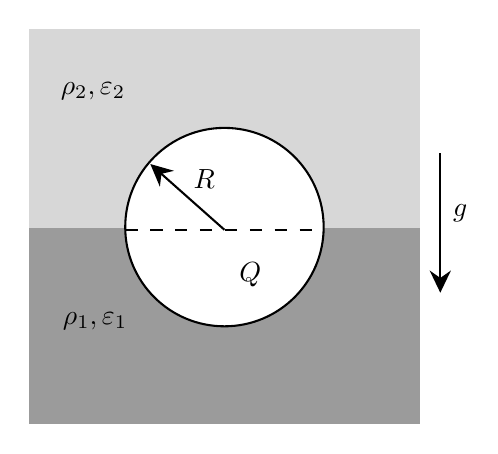
\begin{tikzpicture}[x=0.75pt,y=0.75pt,yscale=-1,xscale=1]
%uncomment if require: \path (0,493); %set diagram left start at 0, and has height of 493

%Shape: Rectangle [id:dp05567602140903616] 
\draw  [draw opacity=0][fill={rgb, 255:red, 155; green, 155; blue, 155 }  ,fill opacity=0.4 ] (192,112) -- (380.6,112) -- (380.6,208.15) -- (192,208.15) -- cycle ;
%Shape: Rectangle [id:dp3819912679054587] 
\draw  [draw opacity=0][fill={rgb, 255:red, 155; green, 155; blue, 155 }  ,fill opacity=1 ] (192,208.15) -- (380.6,208.15) -- (380.6,302.6) -- (192,302.6) -- cycle ;
%Shape: Circle [id:dp693137630346703] 
\draw  [fill={rgb, 255:red, 255; green, 255; blue, 255 }  ,fill opacity=1 ] (238.5,207.58) .. controls (238.5,181.18) and (259.9,159.78) .. (286.3,159.78) .. controls (312.7,159.78) and (334.1,181.18) .. (334.1,207.58) .. controls (334.1,233.97) and (312.7,255.38) .. (286.3,255.38) .. controls (259.9,255.38) and (238.5,233.97) .. (238.5,207.58) -- cycle ;
%Straight Lines [id:da46189804678899193] 
\draw  [dash pattern={on 4.5pt off 4.5pt}]  (238.5,208.88) -- (334.1,208.88) ;
%Straight Lines [id:da1547899101563568] 
\draw    (286.3,208.88) -- (252.84,179.19) ;
\draw [shift={(250.6,177.2)}, rotate = 401.58000000000004] [fill={rgb, 255:red, 0; green, 0; blue, 0 }  ][line width=0.08]  [draw opacity=0] (10.72,-5.15) -- (0,0) -- (10.72,5.15) -- (7.12,0) -- cycle    ;
%Straight Lines [id:da7610915393023661] 
\draw    (390.3,171.88) -- (390.3,236.2) ;
\draw [shift={(390.3,239.2)}, rotate = 270] [fill={rgb, 255:red, 0; green, 0; blue, 0 }  ][line width=0.08]  [draw opacity=0] (10.72,-5.15) -- (0,0) -- (10.72,5.15) -- (7.12,0) -- cycle    ;


% Text Node
\draw (206,136.4) node [anchor=north west][inner sep=0.75pt]    {$\rho_{2} ,\varepsilon_{2}$};
% Text Node
\draw (207,247.4) node [anchor=north west][inner sep=0.75pt]    {$\rho_{1} ,\varepsilon_{1}$};
% Text Node
\draw (270,178.4) node [anchor=north west][inner sep=0.75pt]    {$R$};
% Text Node
\draw (292,223.4) node [anchor=north west][inner sep=0.75pt]    {$Q$};
% Text Node
\draw (395,195.4) node [anchor=north west][inner sep=0.75pt]    {$\ot{g}$};


\end{tikzpicture}
    \end{center}
    \begin{enumerate}[a)]
        \item Xác định vector cường độ điện trường trong toàn không gian, mật độ điện tích tự do ${{\sigma}_{f}}$ ở mặt cầu và mật độ điện tích liên kết mặt ${{\sigma }_{b}}$ ở mặt phân cách giữa quả cầu và hai lớp điện môi theo $R,~{{\varepsilon }_{0}},~{{\varepsilon }_{1}},~{{\varepsilon }_{2}},~Q$.
        \item Tìm lực tĩnh điện tác dụng lên quả cầu theo $R,~{{\varepsilon }_{0}},~{{\varepsilon }_{1}},~{{\varepsilon }_{2}},~Q.$
        \item Tìm $Q$ theo $\rho ,~{{\rho }_{1}},~{{\rho }_{2}},~R,~{{\varepsilon }_{0}},~{{\varepsilon }_{1}},~{{\varepsilon }_{2}},~g.$
    \end{enumerate}
\end{enumerate}
\textbf{Gợi ý:}
\begin{itemize}
    \item Trong tĩnh điện học, ta có phương trình Maxwell $\ot{\nabla }\times \ot{E}=0$. Dùng hệ tọa độ cầu $(r,\theta ,\varphi )$, vector $\ot{\nabla }\times \ot{E}$ có các thành phần sau: 
    \begin{itemize}
        \item Thành phần theo tọa độ $r$: $\dfrac{1}{r\sin \theta }\left[ \dfrac{\partial }{\partial \theta }\left( {{E}_{\varphi }}\sin \theta  \right)-\dfrac{\partial {{E}_{\theta }}}{\partial \varphi } \right]$;
        \item Thành phần theo tọa độ $\theta $: $\dfrac{1}{r\sin \theta }\dfrac{\partial {{E}_{r}}}{\partial \varphi }-\dfrac{1}{r}\dfrac{\partial \left( r{{E}_{\varphi }} \right)}{\partial r}$;
        \item Thành phần theo tọa độ $\varphi $: $\dfrac{1}{r}\left[ \dfrac{\partial \left( r{{E}_{\theta }} \right)}{\partial r}-\dfrac{\partial {{E}_{r}}}{\partial \theta } \right]$.
    \end{itemize}
    \item Có thể sử dụng các công thức
    \begin{itemize}
        \item $\ot{P}={{\varepsilon }_{0}}(\varepsilon -1)\ot{E}$;
        \item ${{\sigma }_{b}}=\ot{P}\cdot\ot{n}$.
    \end{itemize} 
    Trong đó, $\ot{P}$ là vector phân cực, $\ot{n}$ là vector pháp tuyến của mặt phân cách hai môi trường.
\end{itemize}
\end{vd}
\begin{loigiai}
    \begin{enumerate}[1)]
        \item \begin{enumerate}[a)]
            \item Xét lớp cầu rất mỏng có diện tích $\dd S=2\pi R_{1}^{2}\sin \theta \dd \theta $, điện tích lớp cầu $$\dd q=\left( \dfrac{q}{4\pi R_{1}^{2}} \right)2\pi R_{1}^{2}\sin \theta \dd\theta.$$
            \begin{center}
                \tikzset{every picture/.style={line width=0.75pt}} %set default line width to 0.75pt        
                
                 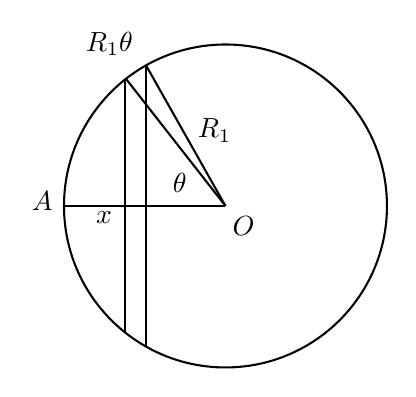
\begin{tikzpicture}[x=0.75pt,y=0.75pt,yscale=-1,xscale=1]
                %uncomment if require: \path (0,484); %set diagram left start at 0, and has height of 484
                
                %Shape: Circle [id:dp18562832027574871] 
                \draw   (228,199.8) .. controls (228,156.83) and (262.83,122) .. (305.8,122) .. controls (348.77,122) and (383.6,156.83) .. (383.6,199.8) .. controls (383.6,242.77) and (348.77,277.6) .. (305.8,277.6) .. controls (262.83,277.6) and (228,242.77) .. (228,199.8) -- cycle ;
                %Straight Lines [id:da16463864413144247] 
                \draw    (228,199.8) -- (305.8,199.8) ;
                %Straight Lines [id:da8825108875983956] 
                \draw    (267.6,132.2) -- (305.8,199.8) ;
                %Straight Lines [id:da698449191179044] 
                \draw    (257.6,138.2) -- (305.8,199.8) ;
                %Straight Lines [id:da05966858398450525] 
                \draw    (257.6,139.2) -- (257.6,261.2) ;
                %Straight Lines [id:da03653987721386809] 
                \draw    (267.6,132.2) -- (267.6,267.2) ;
                
                
                % Text Node
                \draw (291,156.4) node [anchor=north west][inner sep=0.75pt]    {$R_{1}$};
                % Text Node
                \draw (237,114.4) node [anchor=north west][inner sep=0.75pt]    {$R_{1} \dd\theta $};
                % Text Node
                \draw (211,191.4) node [anchor=north west][inner sep=0.75pt]    {$A$};
                % Text Node
                \draw (242,200.9) node [anchor=north west][inner sep=0.75pt]    {$x$};
                % Text Node
                \draw (307.8,203.2) node [anchor=north west][inner sep=0.75pt]    {$O$};
                % Text Node
                \draw (279,182.4) node [anchor=north west][inner sep=0.75pt]    {$\theta $};
                
                \end{tikzpicture}
            \end{center}
            Điện trường tại $A$ theo hướng $OA$ (hình vẽ) do điện tích $\dd q$ gây ra là:
            \[\begin{aligned}
                \dd{{E}_{A}} &= \dfrac{1}{4\pi {{\varepsilon }_{0}}}\dfrac{\dd q\cdot x}{{{\left( R_{1}^{2}{{\sin }^{2}}\theta +{{x}^{2}} \right)}^{3/2}}}=\dfrac{1}{4\pi {{\varepsilon }_{0}}}\dfrac{\left( \dfrac{q}{4\pi R_{1}^{2}} \right)2\pi R_{1}^{2}\sin \theta \dd \theta \cdot {{R}_{1}}(1-\cos \theta )}{{{\left[ R_{1}^{2}{{\sin }^{2}}\theta +R_{1}^{2}{{(1-\cos \theta )}^{2}} \right]}^{3/2}}},\\
                \dd{{E}_{A}} &= \dfrac{1}{4\pi {{\varepsilon }_{0}}}\dfrac{\left( \dfrac{q}{4\pi R_{1}^{2}} \right)2\pi R_{1}^{2}\sin \theta \dd \theta }{{{\left( 2{{R}_{1}}\sin \dfrac{\theta }{2} \right)}^{2}}}\sin \dfrac{\theta }{2}=\dfrac{\dfrac{q}{4\pi R_{1}^{2}}}{2{{\varepsilon }_{0}}}\cos \dfrac{\theta }{2}~\dd\dfrac{\theta }{2}.\\
                {{E}_{A}} &= \dfrac{q/4\pi R_{1}^{2}}{2{{\varepsilon }_{0}}}\int_{0}^{\pi }{\cos }\dfrac{\theta }{2}~\dd\dfrac{\theta }{2}=\dfrac{q/4\pi R_{1}^{2}}{2{{\varepsilon }_{0}}}.
            \end{aligned}\]
            
            Áp suất tĩnh điện lên bề mặt của bong bóng xà phòng: 
            $$P=\dfrac{q}{4\pi R_{1}^{2}}{{E}_{A}}=\dfrac{{{\left( q/4\pi R_{1}^{2} \right)}^{2}}}{2{{\varepsilon }_{0}}}.$$
            \item Gọi $P_{i}'$ và $\rho_{i}'$ là áp suất và mật độ mới của khí trong bóng bóng. $P_{i}'$ liên hệ với áp suất ban đầu ${{P}_{i}}$ theo định luật khí lí tưởng
            \[\left. \begin{aligned}
            \dfrac{4}{3}\pi R_1^3P_i^\prime  &= \dfrac{4}{3}\pi R_0^3{P_i} \\
             {P_i} &= {P_a} + \dfrac{{4\gamma }}{{{R_0}}}
            \end{aligned}  \right\} \Rightarrow P_i^\prime  = \left( {\dfrac{{R_0^3}}{{R_1^3}}} \right)\left( {{P_a} + \dfrac{{4\gamma }}{{{R_0}}}} \right). \label{tft19.1.1}\tag{1}\]
            
            Phương trình xác định bán kính mới ${{R}_{1}}$, điều kiện cân bằng nhiệt cả bong bóng xà phòng \[P_{i}^{\prime }=-\dfrac{{{q}^{2}}}{32{{\varepsilon }_{0}}{{\pi }^{2}}R_{1}^{4}}+{{P}_{a}}+\dfrac{4\gamma }{{{R}_{1}}}. \tag{2} \label{tft19.1.2}\]
            Thay (\ref{tft19.1.1}) vào (\ref{tft19.1.2}), tìm được:
            \[{{\left( \dfrac{{{R}_{1}}}{{{R}_{0}}} \right)}^{4}}+\dfrac{4\gamma }{{{P}_{a}}{{R}_{0}}}{{\left( \dfrac{{{R}_{1}}}{{{R}_{0}}} \right)}^{3}}-\dfrac{{{R}_{1}}}{{{R}_{0}}}\left( 1+\dfrac{4\gamma }{{{P}_{a}}{{R}_{0}}} \right)=\dfrac{{{q}^{2}}}{32{{\varepsilon }_{0}}{{\pi }^{2}}R_{0}^{4}{{P}_{a}}}. \tag{*}\label{tft19.1.3}\]
            Vì $\dfrac{{{q}^{2}}}{{{P}_{a}}{{\varepsilon }_{0}}R_{0}^{4}}\ll 1,~\Delta R={{R}_{1}}-{{R}_{0}}\ll {{R}_{0}}.$
            \\Ta có: \[\dfrac{{{R}_{1}}}{{{R}_{0}}}=\dfrac{{{R}_{0}}+\Delta R}{{{R}_{0}}}=1+\dfrac{\Delta R}{{{R}_{0}}};{{\left( \dfrac{{{R}_{1}}}{{{R}_{0}}} \right)}^{3}}\approx 1+3\dfrac{\Delta R}{{{R}_{0}}};{{\left( \dfrac{{{R}_{1}}}{{{R}_{0}}} \right)}^{4}}\approx 1+4\dfrac{\Delta R}{{{R}_{0}}}.\]
            Thay vào (\ref{tft19.1.3}) ta tìm được:
            \[
            \begin{aligned}
                &1+4\dfrac{\Delta R}{{{R}_{0}}}+\dfrac{4\gamma }{{{P}_{a}}{{R}_{0}}}\left( 1+3\dfrac{\Delta R}{{{R}_{0}}} \right)-\left( 1+\dfrac{\Delta R}{{{R}_{0}}} \right)\left( 1+\dfrac{4\gamma }{{{P}_{a}}{{R}_{0}}} \right) = \dfrac{{{q}^{2}}}{32{{\varepsilon }_{0}}{{\pi }^{2}}R_{0}^{4}{{P}_{a}}}\\
                &\Leftrightarrow 3\dfrac{\Delta R}{{{R}_{0}}}\left( 1+\dfrac{2}{3}\dfrac{4\gamma }{{{P}_{a}}{{R}_{0}}} \right) = \dfrac{{{q}^{2}}}{32{{\varepsilon }_{0}}{{\pi }^{2}}R_{0}^{4}{{P}_{a}}} \\
                &\Leftrightarrow \Delta R = {{R}_{0}}\dfrac{{{q}^{2}}}{96{{\varepsilon }_{0}}{{\pi }^{2}}R_{0}^{4}{{P}_{a}}\left( 1+\dfrac{2}{3}\dfrac{4\gamma }{{{P}_{o}}{{R}_{0}}} \right)}. 
            \end{aligned}\]
            \item Bong bóng đứng yên trong không khí khi: \[-\pi R_{1}^{3}{{\rho }_{a}}g=4\pi R_{0}^{2}{{\rho }_{s}}tg+\dfrac{4}{3}\pi R_{0}^{3}{{\rho }_{i}}g,\]
            trong đó ${{\rho }_{i}}={{\rho }_{a}}\left( 1+\dfrac{4\gamma }{{{P}_{o}}{{R}_{0}}} \right),~ {{R}_{1}}={{R}_{0}}\left( 1+\dfrac{\Delta R}{{{R}_{0}}} \right).$
            \\Thay vào công thức trên, ta có:
            \[\begin{aligned}
                \dfrac{4}{3}\pi R_{0}^{3}{{\left( 1+\dfrac{\Delta R}{{{R}_{0}}} \right)}^{3}}{{\rho }_{a}}g &= 4\pi R_{0}^{2}{{\rho }_{s}}tg+\dfrac{4}{3}\pi R_{0}^{3}{{\rho }_{a}}\left( 1+\dfrac{4\gamma }{{{P}_{a}}{{R}_{0}}} \right)g \\
                {{R}_{0}}\left( 1+3\dfrac{\Delta R}{{{R}_{0}}} \right){{\rho }_{a}} &= 3{{\rho }_{s}}t+{{R}_{0}}{{\rho }_{a}}\left( 1+\dfrac{4\gamma }{{{P}_{a}}{{R}_{0}}} \right)\\
               \Delta R &=\dfrac{{{\rho }_{s}}}{{{\rho }_{a}}}t+\dfrac{4\gamma }{3{{P}_{o}}}.
            \end{aligned}            \]
            Điện tích $q$ được tính theo công thức:
            \[{{q}^{2}}=96{{\varepsilon }_{0}}{{\pi }^{2}}R_{0}^{3}{{P}_{a}}\left( 1+\dfrac{2}{3}\dfrac{4\gamma }{{{P}_{a}}{{R}_{0}}} \right)\left( \dfrac{{{\rho }_{s}}}{{{\rho }_{a}}}t+\dfrac{4\gamma }{3{{P}_{a}}} \right)\]
            \[\Rightarrow q=\sqrt{96{{\varepsilon }_{0}}{{\pi }^{2}}R_{0}^{3}{{P}_{a}}\left( 1+\dfrac{2}{3}\dfrac{4\gamma }{{{P}_{a}}{{R}_{0}}} \right)\left( \dfrac{{{\rho }_{s}}}{{{\rho }_{a}}}t+\dfrac{4\gamma }{3{{P}_{a}}} \right)}.\]
            Thay số, ta tìm được: 
            \[q=9.6737.10^{-9}~\mathrm{C}.\]
            \end{enumerate}
            \item    \begin{enumerate}[a)]
                \item Ta sẽ dùng tọa độ cầu $(r,\theta ,\varphi )$, với gốc $O$ ở tâm quả cầu và trục $z$ vuông góc với mặt phân cách của hai chất điện môi (Hình vẽ). Điện trường trong vật dẫn bằng không. Kí hiệu điện trường bên ngoài quả cầu là $\ot{E}(r,\theta ,\varphi )$, nó độc lập với $\varphi $ do tính chất đối xứng cầu.
        \begin{center}
            \tikzset{every picture/.style={line width=0.5pt}} %set default line width to 0.75pt        
            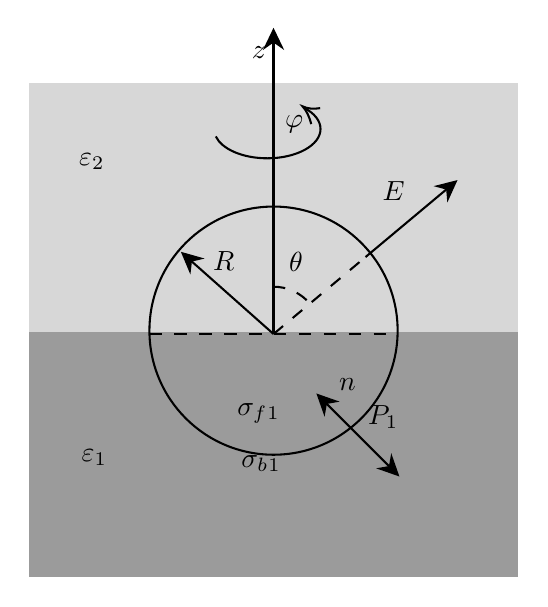
\begin{tikzpicture}[x=0.75pt,y=0.75pt,yscale=-1,xscale=1]
            \draw  [draw opacity=0][fill={rgb, 255:red, 155; green, 155; blue, 155 }  ,fill opacity=0.4 ] (212,84.2) -- (447.9,84.2) -- (447.9,204.46) -- (212,204.46) -- cycle ;
            \draw  [draw opacity=0][fill={rgb, 255:red, 155; green, 155; blue, 155 }  ,fill opacity=1 ] (212,204.46) -- (447.9,204.46) -- (447.9,322.6) -- (212,322.6) -- cycle ;
            \draw   (270.16,203.74) .. controls (270.16,170.72) and (296.93,143.96) .. (329.95,143.96) .. controls (362.97,143.96) and (389.74,170.72) .. (389.74,203.74) .. controls (389.74,236.76) and (362.97,263.53) .. (329.95,263.53) .. controls (296.93,263.53) and (270.16,236.76) .. (270.16,203.74) -- cycle ;
            \draw  [dash pattern={on 4.5pt off 4.5pt}]  (270.16,205.37) -- (389.74,205.37) ;
            \draw    (329.95,205.37) -- (287.54,167.74) ;
            \draw [shift={(285.3,165.75)}, rotate = 401.58000000000004] [fill={rgb, 255:red, 0; green, 0; blue, 0 }  ][line width=0.08]  [draw opacity=0] (10.72,-5.15) -- (0,0) -- (10.72,5.15) -- (7.12,0) -- cycle    ;
            \draw    (329.95,205.37) -- (329.95,60.83) ;
            \draw [shift={(329.95,57.83)}, rotate = 450] [fill={rgb, 255:red, 0; green, 0; blue, 0 }  ][line width=0.08]  [draw opacity=0] (10.72,-5.15) -- (0,0) -- (10.72,5.15) -- (7.12,0) -- cycle    ;
            \draw    (374.27,168.29) -- (416.3,133.13) ;
            \draw [shift={(418.6,131.2)}, rotate = 500.08] [fill={rgb, 255:red, 0; green, 0; blue, 0 }  ][line width=0.08]  [draw opacity=0] (10.72,-5.15) -- (0,0) -- (10.72,5.15) -- (7.12,0) -- cycle    ;
            \draw  [dash pattern={on 4.5pt off 4.5pt}]  (329.95,205.37) -- (374.27,168.29) ;
            \draw    (366.95,250.37) -- (352.72,236.14) ;
            \draw [shift={(350.6,234.02)}, rotate = 405] [fill={rgb, 255:red, 0; green, 0; blue, 0 }  ][line width=0.08]  [draw opacity=0] (10.72,-5.15) -- (0,0) -- (10.72,5.15) -- (7.12,0) -- cycle    ;
            \draw    (366.95,250.37) -- (388.48,271.9) ;
            \draw [shift={(390.6,274.02)}, rotate = 225] [fill={rgb, 255:red, 0; green, 0; blue, 0 }  ][line width=0.08]  [draw opacity=0] (10.72,-5.15) -- (0,0) -- (10.72,5.15) -- (7.12,0) -- cycle    ;
            \draw  [draw opacity=0][dash pattern={on 4.5pt off 4.5pt}] (329.61,182.58) .. controls (332.91,182.53) and (336.27,183.2) .. (339.47,184.67) .. controls (343.15,186.36) and (346.17,188.91) .. (348.39,191.98) -- (329.95,205.37) -- cycle ; \draw  [dash pattern={on 4.5pt off 4.5pt}] (329.61,182.58) .. controls (332.91,182.53) and (336.27,183.2) .. (339.47,184.67) .. controls (343.15,186.36) and (346.17,188.91) .. (348.39,191.98) ;
            \draw  [draw opacity=0] (344.69,96.39) .. controls (349.56,98.96) and (352.59,102.57) .. (352.59,106.58) .. controls (352.6,114.38) and (341.12,120.7) .. (326.96,120.71) .. controls (315.04,120.72) and (305.02,116.25) .. (302.14,110.18) -- (326.95,106.59) -- cycle ; \draw   (344.69,96.39) .. controls (349.56,98.96) and (352.59,102.57) .. (352.59,106.58) .. controls (352.6,114.38) and (341.12,120.7) .. (326.96,120.71) .. controls (315.04,120.72) and (305.02,116.25) .. (302.14,110.18) ;
            \draw  [line width=0.75]  (352.42,96.54) .. controls (349.11,97.1) and (346.27,96.81) .. (343.91,95.66) .. controls (345.79,97.67) and (347.18,100.52) .. (348.1,104.24) ;
            
            \draw (234.78,116.88) node [anchor=north west][inner sep=0.75pt]    {$\varepsilon _{2}$};
            \draw (236.03,259.71) node [anchor=north west][inner sep=0.75pt]    {$\varepsilon _{1}$};
            \draw (299.32,164.16) node [anchor=north west][inner sep=0.75pt]    {$R$};
            \draw (381,130.4) node [anchor=north west][inner sep=0.75pt]    {$\ot{E}$};
            \draw (318,65.4) node [anchor=north west][inner sep=0.75pt]    {$z$};
            \draw (336,164.4) node [anchor=north west][inner sep=0.75pt]    {$\theta $};
            \draw (311,237.4) node [anchor=north west][inner sep=0.75pt]    {$\sigma _{f}{}_{1}$};
            \draw (313,262.4) node [anchor=north west][inner sep=0.75pt]    {$\sigma _{b}{}_{1}$};
            \draw (360,225.4) node [anchor=north west][inner sep=0.75pt]    {$\ot{n}$};
            \draw (374,238.4) node [anchor=north west][inner sep=0.75pt]    {$\ot{P_{1}}$};
            \draw (334,98.4) node [anchor=north west][inner sep=0.75pt]    {$\varphi $};
            
            
            \end{tikzpicture}
        \end{center}
        Do quả cầu dẫn điện nên nó là mặt đẳng thế, vì vậy điện trường ở ngay sát bên ngoài của mặt cầu, tức là $\ot{E}({{R}^{+}},\theta ,\varphi )$, phải vuông góc với mặt đó. Nghĩa là điện trường này tại sát mặt cầu chỉ có thành phần ${{E}_{r}}$, hay ở gần biên ta có ${{E}_{\varphi }}=0,{{E}_{\theta }}=0$. Vậy nếu viết phương trình Maxwell $\ot{\nabla }\times \ot{E}=0$ trong tọa độ cầu ở lân cận mặt cầu $r={{R}^{+}}$ ta thấy rằng thành phần theo $\varphi ,\theta $ sẽ tự động bằng không do ${{E}_{\varphi }}=0,{{E}_{\theta }}=0$. Và tất cả các đạo hàm theo $\varphi $ bằng không. Điều kiện để các thành phần theo $\varphi $ của $\ot{\nabla }\times \ot{E}=0$ là:
        \[\begin{aligned}
            &~~\dfrac{1}{r}\left[ \dfrac{\partial \left( r{{E}_{\theta }} \right)}{\partial r}-\dfrac{\partial {{E}_{r}}}{\partial \theta } \right]=0\\
            &\Rightarrow \dfrac{\partial \left( r{{E}_{\theta }} \right)}{\partial r}-\dfrac{\partial {{E}_{r}}}{\partial \theta }=0\\
            &\Rightarrow \dfrac{\partial {{E}_{r}}}{\partial \theta }=\dfrac{\partial \left( r{{E}_{\theta }} \right)}{\partial r}={{E}_{\theta }}+r\dfrac{\partial \left( {{E}_{\theta }} \right)}{\partial r}.
        \end{aligned}
        \]
        Vế phải ở gần mặt cầu bằng không, vì ${{E}_{\theta }}\left( {{R}^{-}} \right)={{E}_{\theta }}\left( {{R}^{+}} \right)=0$ (do thành phần song song của điện trường liên tục qua biên). Suy ra ${{\left. \dfrac{\partial \left( {{E}_{\theta }} \right)}{\partial r} \right|}_{R}}=0$ do đó theo (\ref{tft19.1.3}) ${{\left. \dfrac{\partial \left( {{E}_{r}} \right)}{\partial r} \right|}_{R}}=0$, suy ra ${{E}_{r}}$ không phụ thuộc vào $\theta $.
        \\Kí hiệu ${{\sigma }_{\text{tot}}}$ là tổng mật độ điện tích mặt của các điện tích mặt tự do ${{\sigma }_{f}}$ và mật độ điện tích mặt liên kết ${{\sigma }_{b}}$. Ta có:
        \[{{\sigma}_{\text{tot}}}={{\varepsilon }_{0}}E={{\varepsilon }_{0}}E\left( {{R}^{+}},\theta ,\varphi  \right)={{\varepsilon }_{0}}E\left( {{R}^{+}} \right).\]
        Như vậy mật độ điện tích mặt ${{\sigma }_{\text{tot}}}$ như nhau trên toàn mặt cầu. Do đó điện trường ở bên ngoài của quả cầu bằng điện trường của một điện tích điểm đặt tại $O$ với điện tích ${{Q}_{\text{tot}}}=Q+{{Q}_{b}}$, cụ thể là:
        \[\ot{E}(r,\theta ,\varphi )=\ot{E}(r)=\dfrac{1}{4\pi {{\varepsilon }_{0}}}\dfrac{{{Q}_{\text{tot}}}}{{{r}^{3}}}\ot{r}=\dfrac{1}{4\pi {{\varepsilon }_{0}}}\dfrac{4\pi {{R}^{2}}{{\sigma }_{\text{tot}}}}{{{r}^{3}}}\ot{r}=\dfrac{1}{{{\varepsilon }_{0}}}{{\sigma }_{\text{tot }}}{{\left( \dfrac{R}{r} \right)}^{2}}\dfrac{{\ot{r}}}{r}, \label{**}\]
        vì điện trường chỉ phụ thuộc vào $r$.
        \\Theo công thức trong đề bài thì mật độ điện tích liên kết (phân cực) ở bề mặt của hai chất điện môi tiếp xúc với quả cầu lần lượt là:
            \[\left\{ \begin{aligned}
          {\sigma _{b1}} &= \ot n{{\ot{P_1}}} =  - \left( {{\varepsilon _1} - 1} \right){\varepsilon _0}E(R) =  - \left( {{\varepsilon _1} - 1} \right){\sigma _{{\text{tot }}}},  \\
          {\sigma _{b2}} &= \ot n\ot {{P_2}}  =  - \left( {{\varepsilon _2} - 1} \right){\varepsilon _0}E(R) =  - \left( {{\varepsilon _2} - 1} \right){\sigma _{{\text{tot}}}}. 
        \end{aligned}  \right.\]
        Trong đó $\ot{n}=-\dfrac{{\ot{r}}}{r}$, hướng vào tâm quả cầu (hay hướng ra ngoài lớp điện môi).
        Khi đó mật độ các điện tích tự do trên phần mặt cầu tiếp giáp với hai chất điện môi tiếp xúc với quả cầu lần lượt là:
            \[\left\{ \begin{aligned}
          {\sigma _{f1}} &= {\sigma _{{\text{tot }}}} - {\sigma _{b1}} = {\varepsilon _1}{\sigma _{{\text{tot }}}}, \\
          {\sigma _{f2}} &= {\sigma _{{\text{tot}}}} - {\sigma _{b2}} = {\varepsilon _2}{\sigma _{{\text{tot}}}}.
        \end{aligned}  \right.\]
        Mặt khác $2\pi {{R}^{2}}\left( {{\sigma }_{f1}}+{{\sigma }_{f2}} \right)=Q$, suy ra:
        \[{{\sigma }_{\text{tot }}}=\dfrac{Q}{2\pi {{R}^{2}}\left( {{\varepsilon }_{1}}+{{\varepsilon }_{2}} \right)}.\]
        \[\ot{E}(r)=\left\{ \begin{aligned}
        \dfrac{1}{2\pi {{\varepsilon }_{0}}}\dfrac{Q}{\left( {{\varepsilon }_{1}}+{{\varepsilon }_{2}} \right){{r}^{2}}}\ot{r}\quad  & r\ge R,  \\
         0 \quad & 0<r<R. 
        \end{aligned} \right.\]
            
            \[\left\{ \begin{gathered}
          {\sigma _{f1}} = \dfrac{{{\varepsilon _1}Q}}{{2\pi {R^2}\left( {{\varepsilon _1} + {\varepsilon _2}} \right)}}, \hfill \\
          {\sigma _{f2}} = \dfrac{{{\varepsilon _2}Q}}{{2\pi {R^2}\left( {{\varepsilon _1} + {\varepsilon _2}} \right)}} .\hfill \\ 
        \end{gathered}  \right.~~~~~~\left\{ \begin{gathered}
          {\sigma _{b1}} =  - \dfrac{{\left( {{\varepsilon _1} - 1} \right)Q}}{{2\pi {R^2}\left( {{\varepsilon _1} + {\varepsilon _2}} \right)}}, \hfill \\
          {\sigma _{b2}} =  - \dfrac{{\left( {{\varepsilon _2} - 1} \right)Q}}{{2\pi {R^2}\left( {{\varepsilon _1} + {\varepsilon _2}} \right)}}. \hfill \\ 
        \end{gathered}  \right.\]
        \item Áp dụng $P=\dfrac{1}{2}\dfrac{{{\sigma }^{2}}}{{{\varepsilon }_{0}}\varepsilon }$, áp suất tĩnh điện trên bề mặt hai nửa bán cầu trong môi trường điện môi  $${{P}_{fi}}=\dfrac{1}{2}\dfrac{\sigma _{fi}^{2}}{{{\varepsilon }_{0}}{{\varepsilon }_{i}}}=\dfrac{1}{2{{\varepsilon }_{i}}{{\varepsilon }_{0}}}{{\left[ \dfrac{{{\varepsilon }_{i}}Q}{2\pi {{R}^{2}}\left( {{\varepsilon }_{1}}+{{\varepsilon }_{2}} \right)} \right]}^{2}}$$, với $i=1,2$. 
        \\Vì ${{\varepsilon }_{1}}>{{\varepsilon }_{2}}\Rightarrow {{P}_{1}}>{{P}_{2}}$ nên áp suất này sẽ đẩy quả cầu về phía môi trường có hằng số điện môi lớn hơn.
        \\Lực tác dụng lên yếu tố điện tích $\dd S={{R}^{2}}\sin \theta \dd\theta \dd\varphi $ bằng $\dd\ot{F}=P\dd S\ot{r}$, với $i=1$ nếu $\theta >\dfrac{\pi }{2}$;  $i=2$ nếu $\theta <\dfrac{\pi }{2}$ (Hình vẽ).
        \begin{center}
            \tikzset{every picture/.style={line width=0.75pt}} %set default line width to 0.75pt        
            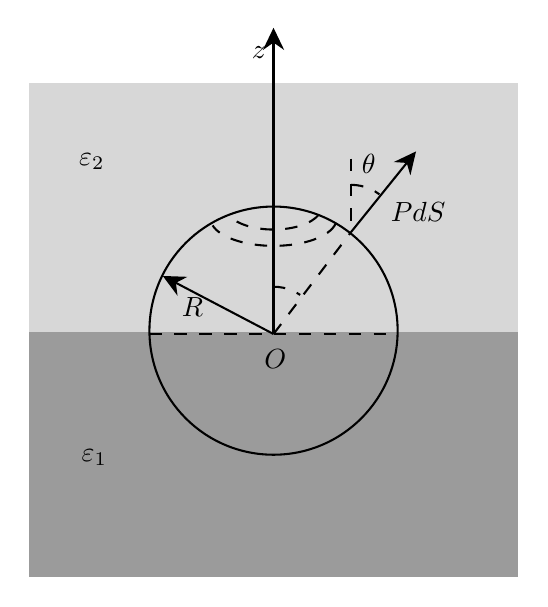
\begin{tikzpicture}[x=0.75pt,y=0.75pt,yscale=-1,xscale=1]
            \draw  [draw opacity=0][fill={rgb, 255:red, 155; green, 155; blue, 155 }  ,fill opacity=0.4 ] (212,84.2) -- (447.9,84.2) -- (447.9,204.46) -- (212,204.46) -- cycle ;
            \draw  [draw opacity=0][fill={rgb, 255:red, 155; green, 155; blue, 155 }  ,fill opacity=1 ] (212,204.46) -- (447.9,204.46) -- (447.9,322.6) -- (212,322.6) -- cycle ;
            \draw   (270.16,203.74) .. controls (270.16,170.72) and (296.93,143.96) .. (329.95,143.96) .. controls (362.97,143.96) and (389.74,170.72) .. (389.74,203.74) .. controls (389.74,236.76) and (362.97,263.53) .. (329.95,263.53) .. controls (296.93,263.53) and (270.16,236.76) .. (270.16,203.74) -- cycle ;
            \draw  [dash pattern={on 4.5pt off 4.5pt}]  (270.16,205.37) -- (389.74,205.37) ;
            \draw    (329.95,205.37) -- (279.26,178.79) ;
            \draw [shift={(276.6,177.4)}, rotate = 387.66999999999996] [fill={rgb, 255:red, 0; green, 0; blue, 0 }  ][line width=0.08]  [draw opacity=0] (10.72,-5.15) -- (0,0) -- (10.72,5.15) -- (7.12,0) -- cycle    ;
            \draw    (329.95,205.37) -- (329.95,60.83) ;
            \draw [shift={(329.95,57.83)}, rotate = 450] [fill={rgb, 255:red, 0; green, 0; blue, 0 }  ][line width=0.08]  [draw opacity=0] (10.72,-5.15) -- (0,0) -- (10.72,5.15) -- (7.12,0) -- cycle    ;
            \draw    (367.27,156.29) -- (396.72,119.74) ;
            \draw [shift={(398.6,117.4)}, rotate = 488.85] [fill={rgb, 255:red, 0; green, 0; blue, 0 }  ][line width=0.08]  [draw opacity=0] (10.72,-5.15) -- (0,0) -- (10.72,5.15) -- (7.12,0) -- cycle    ;
            \draw  [dash pattern={on 4.5pt off 4.5pt}]  (329.95,205.37) -- (367.27,156.29) ;
            \draw  [draw opacity=0][dash pattern={on 4.5pt off 4.5pt}][line width=0.75]  (329.61,182.58) .. controls (332.91,182.53) and (336.27,183.2) .. (339.47,184.67) .. controls (340.64,185.21) and (341.75,185.83) .. (342.78,186.53) -- (329.95,205.37) -- cycle ; \draw  [dash pattern={on 4.5pt off 4.5pt}][line width=0.75]  (329.61,182.58) .. controls (332.91,182.53) and (336.27,183.2) .. (339.47,184.67) .. controls (340.64,185.21) and (341.75,185.83) .. (342.78,186.53) ;
            \draw  [draw opacity=0][dash pattern={on 4.5pt off 4.5pt}] (351.78,147.83) .. controls (348.48,152.04) and (339.95,155.04) .. (329.95,155.04) .. controls (319.48,155.04) and (310.63,151.76) .. (307.69,147.24) -- (329.95,143.96) -- cycle ; \draw  [dash pattern={on 4.5pt off 4.5pt}] (351.78,147.83) .. controls (348.48,152.04) and (339.95,155.04) .. (329.95,155.04) .. controls (319.48,155.04) and (310.63,151.76) .. (307.69,147.24) ;
            \draw  [draw opacity=0][dash pattern={on 4.5pt off 4.5pt}] (359.81,152.33) .. controls (356.97,158.36) and (344.71,162.9) .. (330.02,162.9) .. controls (315.92,162.9) and (304.06,158.72) .. (300.61,153.05) -- (330.02,149.65) -- cycle ; \draw  [dash pattern={on 4.5pt off 4.5pt}] (359.81,152.33) .. controls (356.97,158.36) and (344.71,162.9) .. (330.02,162.9) .. controls (315.92,162.9) and (304.06,158.72) .. (300.61,153.05) ;
            \draw  [dash pattern={on 4.5pt off 4.5pt}]  (367.27,120.89) -- (367.27,156.29) ;
            \draw  [draw opacity=0][dash pattern={on 4.5pt off 4.5pt}][line width=0.75]  (367.26,133.49) .. controls (370.45,133.49) and (373.7,134.16) .. (376.8,135.58) .. controls (378.31,136.28) and (379.71,137.12) .. (380.99,138.08) -- (367.27,156.29) -- cycle ; \draw  [dash pattern={on 4.5pt off 4.5pt}][line width=0.75]  (367.26,133.49) .. controls (370.45,133.49) and (373.7,134.16) .. (376.8,135.58) .. controls (378.31,136.28) and (379.71,137.12) .. (380.99,138.08) ;
            \draw (234.78,116.88) node [anchor=north west][inner sep=0.75pt]    {$\varepsilon _{2}$};
            \draw (236.03,259.71) node [anchor=north west][inner sep=0.75pt]    {$\varepsilon _{1}$};
            \draw (284.32,186.16) node [anchor=north west][inner sep=0.75pt]    {$R$};
            \draw (318,65.4) node [anchor=north west][inner sep=0.75pt]    {$z$};
            \draw (371,117.4) node [anchor=north west][inner sep=0.75pt]    {$\theta $};
            \draw (324,211.4) node [anchor=north west][inner sep=0.75pt]    {$O$};
            \draw (384.94,140.24) node [anchor=north west][inner sep=0.75pt]    {$\ot{P} dS$};
            \end{tikzpicture}
        \end{center}
            Lực tổng hợp tác dụng lên nửa mặt cầu bên trên (chỉ có thành phần $z$ là có đóng góp) là:
    $${{\ot{F_2}}}=\ot{z}\int_{0}^{2\pi }{\dd}\varphi \int_{0}^{\pi /2}{\dd}\theta {{R}^{2}}\sin \theta \cos \theta \dfrac{1}{2{{\varepsilon }_{0}}{{\varepsilon }_{2}}}{{\left[ \dfrac{{{\varepsilon }_{2}}Q}{2\pi {{R}^{2}}\left( {{\varepsilon }_{1}}+{{\varepsilon }_{2}} \right)} \right]}^{2}}=\dfrac{1}{4\pi {{\varepsilon }_{0}}}\dfrac{{{\varepsilon }_{2}}{{Q}^{2}}}{2{{\left( {{\varepsilon }_{1}}+{{\varepsilon }_{2}} \right)}^{2}}{{R}^{2}}}\ot{z},$$
    với $\ot{z}$ là vector đơn vị của trục $z$. Như vậy lực này hướng lên trên.
    \\Tương tự, lực toàn phần tác dụng lên nửa mặt cầu bên dưới là:
    $${{\ot{F_1}}}= - \ot{z}\int_{0}^{2\pi }{\dd}\varphi \int_{0}^{\pi /2}{\dd}\theta {{R}^{2}}\sin \theta \cos \theta \dfrac{1}{2{{\varepsilon }_{0}}{{\varepsilon }_{1}}}{{\left[ \dfrac{{{\varepsilon }_{1}}Q}{2\pi {{R}^{2}}\left( {{\varepsilon }_{1}}+{{\varepsilon }_{2}} \right)} \right]}^{2}}=-\dfrac{1}{4\pi {{\varepsilon }_{0}}}\dfrac{{{\varepsilon }_{1}}{{Q}^{2}}}{2{{\left( {{\varepsilon }_{1}}+{{\varepsilon }_{2}} \right)}^{2}}{{R}^{2}}}\ot{z}.$$
    Vậy lực điện tác dụng lên quả cầu dẫn là:
    $${\ot{F_{\text{tot}}}}={{\ot{F_{1}}}}+{{\ot{F_{2}}}}=-\dfrac{1}{4\pi {{\varepsilon }_{0}}}\dfrac{\left( {{\varepsilon }_{1}}-{{\varepsilon }_{2}} \right){{Q}^{2}}}{2{{\left( {{\varepsilon }_{1}}+{{\varepsilon }_{2}} \right)}^{2}}{{R}^{2}}}\ot{z}.$$
    \item Quả cầu ở trạng thái cân bằng, $\dfrac{1}{2}$ thể tích của nó chìm trong nước, thì lực điện ${{\ot{F_{\text{tot}}}}}$ cộng trọng lực bằng lực đẩy Archimedes, ta có:
    $$\dfrac{1}{4\pi {{\varepsilon }_{0}}}\dfrac{\left( {{\varepsilon }_{1}}-{{\varepsilon }_{2}} \right){{Q}^{2}}}{2{{\left( {{\varepsilon }_{1}}+{{\varepsilon }_{2}} \right)}^{2}}{{R}^{2}}}+\dfrac{4\pi {{R}^{3}}}{3}\rho g=\dfrac{2\pi {{R}^{3}}}{3}\left( {{\rho }_{1}}+{{\rho }_{2}} \right)g.$$
    $$Q=\sqrt{\dfrac{16{{\pi }^{2}}{{\varepsilon }_{0}}{{\left( {{\varepsilon }_{1}}+{{\varepsilon }_{2}} \right)}^{2}}\left( {{\rho }_{1}}+{{\rho }_{2}}-2\rho  \right)g{{R}^{5}}}{3\left( {{\varepsilon }_{1}}-{{\varepsilon }_{2}} \right)}}.$$

        \end{enumerate}
    \end{enumerate}
    \end{loigiai}
    
\begin{vd}[Từ hóa vật liệu]
    Thực nghiệm cho thấy khi đặt vật liệu từ vào từ trường ngoài có vector cảm ứng từ $\overrightarrow{{{{B}}_{0}}}$ thì vật liệu từ sẽ bị từ hóa. Hiện tượng từ hóa này được mô tả bằng vector độ từ hóa $\overrightarrow{{M}}$ (moment từ trên một đơn vị thể tích vật liệu). Vật liệu bị từ hóa sẽ gây ra cảm ứng từ phụ $\overrightarrow{{{{B}}^{\prime }}}={{\mu }_{0}}\overrightarrow{{M}}$ với ${{\mu}_{0}}$ là độ từ thẩm của chân không, do đó cảm ứng từ tổng cộng trong vật liệu bị từ hóa là $\overrightarrow{{B}}=\overrightarrow{{{{B}}_{0}}}+\overrightarrow{{{{B}}^{\prime }}}$.
    \begin{enumerate}[1)]
        \item Xét một khối vật liệu thuận từ lí tưởng, đồng chất, trụ, bán kính ${R}$ và chiều dài ${L}$ $({L}\gg {R})$, xung quanh dây dẫn (có lớp sơn cách điện) với mật độ đều $n$ vòng trên một đơn vị chiều dài và có dòng điện một chiều cường độ $I$ chạy qua (như hình vẽ). Giả thiết vector $\overrightarrow{{M}}$ và vector cường độ từ trường luôn cùng hướng và không phụ thuộc vào vị trí đang xét. Khi thay đổi cường độ dòng điện một lượng nhỏ $\dd I$, nguồn điện thực hiện một công $\delta {{{W}}_{0}}$, công này một phần làm thay đổi cường độ từ trường ngoài, phần còn lại là công $\delta {{{W}}_{{m}}}$ mà vật liệu từ nhận được.
        \begin{center}
            

\tikzset{every picture/.style={line width=0.75pt}} %set default line width to 0.75pt        

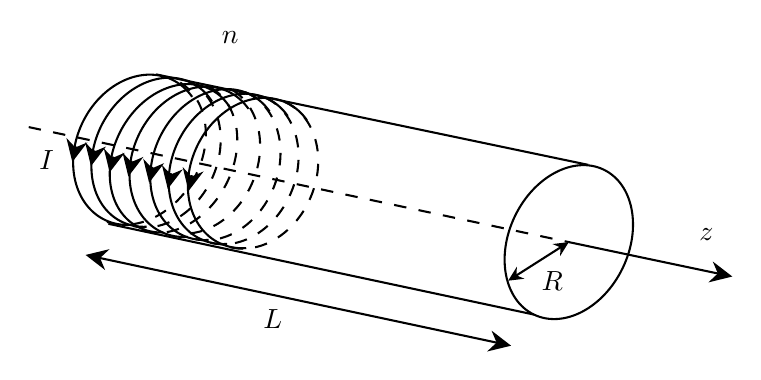
\begin{tikzpicture}[x=0.75pt,y=0.75pt,yscale=-1,xscale=1]
%uncomment if require: \path (0,187); %set diagram left start at 0, and has height of 187

%Shape: Arc [id:dp6351943144867793] 
\draw  [draw opacity=0][dash pattern={on 4.5pt off 4.5pt}] (293.7,47.64) .. controls (308.7,54.32) and (314.28,74.91) .. (306.15,93.81) .. controls (298.01,112.72) and (279.2,122.82) .. (264.03,116.5) -- (278.59,81.95) -- cycle ; \draw  [dash pattern={on 4.5pt off 4.5pt}] (293.7,47.64) .. controls (308.7,54.32) and (314.28,74.91) .. (306.15,93.81) .. controls (298.01,112.72) and (279.2,122.82) .. (264.03,116.5) ;
%Shape: Ellipse [id:dp656203275363282] 
\draw   (404.65,102.71) .. controls (413.94,83.43) and (433.09,73.4) .. (447.43,80.3) .. controls (461.77,87.21) and (465.86,108.44) .. (456.57,127.72) .. controls (447.29,146.99) and (428.14,157.02) .. (413.8,150.12) .. controls (399.46,143.21) and (395.37,121.98) .. (404.65,102.71) -- cycle ;
%Straight Lines [id:da6953963895313522] 
\draw    (231.8,34.4) -- (440,78) ;
%Straight Lines [id:da9157336948337638] 
\draw    (208.8,106.4) -- (413.8,150.12) ;
%Shape: Arc [id:dp41665770987085415] 
\draw  [draw opacity=0][dash pattern={on 4.5pt off 4.5pt}] (284.41,45.68) .. controls (299.29,52.31) and (304.78,72.83) .. (296.66,91.69) .. controls (288.54,110.57) and (269.85,120.69) .. (254.8,114.41) -- (269.34,79.93) -- cycle ; \draw  [dash pattern={on 4.5pt off 4.5pt}] (284.41,45.68) .. controls (299.29,52.31) and (304.78,72.83) .. (296.66,91.69) .. controls (288.54,110.57) and (269.85,120.69) .. (254.8,114.41) ;
%Shape: Arc [id:dp11166627533743312] 
\draw  [draw opacity=0][dash pattern={on 4.5pt off 4.5pt}] (274.65,42.95) .. controls (289.85,49.18) and (296.05,69.59) .. (288.49,88.72) .. controls (280.93,107.88) and (262.44,118.54) .. (247.08,112.67) -- (260.59,77.7) -- cycle ; \draw  [dash pattern={on 4.5pt off 4.5pt}] (274.65,42.95) .. controls (289.85,49.18) and (296.05,69.59) .. (288.49,88.72) .. controls (280.93,107.88) and (262.44,118.54) .. (247.08,112.67) ;
%Shape: Arc [id:dp3408303416739358] 
\draw  [draw opacity=0][dash pattern={on 4.5pt off 4.5pt}] (268.78,42.04) .. controls (281.43,50.02) and (285.7,69.02) .. (278.15,86.56) .. controls (271.13,102.88) and (256.16,112.64) .. (242.44,110.95) -- (250.59,74.7) -- cycle ; \draw  [dash pattern={on 4.5pt off 4.5pt}] (268.78,42.04) .. controls (281.43,50.02) and (285.7,69.02) .. (278.15,86.56) .. controls (271.13,102.88) and (256.16,112.64) .. (242.44,110.95) ;
%Shape: Arc [id:dp47007789626083873] 
\draw  [draw opacity=0][dash pattern={on 4.5pt off 4.5pt}] (257.94,40.76) .. controls (271.75,48.31) and (275.04,69.29) .. (265.26,87.82) .. controls (255.47,106.37) and (236.27,115.48) .. (222.24,108.3) -- (239.82,74.39) -- cycle ; \draw  [dash pattern={on 4.5pt off 4.5pt}] (257.94,40.76) .. controls (271.75,48.31) and (275.04,69.29) .. (265.26,87.82) .. controls (255.47,106.37) and (236.27,115.48) .. (222.24,108.3) ;
%Shape: Arc [id:dp8967166890370217] 
\draw  [draw opacity=0][dash pattern={on 4.5pt off 4.5pt}] (246.7,37.39) .. controls (261.7,44.08) and (267.28,64.66) .. (259.15,83.56) .. controls (251.01,102.48) and (232.2,112.58) .. (217.03,106.25) -- (231.59,71.7) -- cycle ; \draw  [dash pattern={on 4.5pt off 4.5pt}] (246.7,37.39) .. controls (261.7,44.08) and (267.28,64.66) .. (259.15,83.56) .. controls (251.01,102.48) and (232.2,112.58) .. (217.03,106.25) ;
%Shape: Arc [id:dp09936887242710779] 
\draw  [draw opacity=0][dash pattern={on 4.5pt off 4.5pt}] (243.4,38.35) .. controls (257.34,47.08) and (259.86,68.5) .. (248.98,86.37) .. controls (238.1,104.25) and (217.9,111.85) .. (203.74,103.45) -- (223.31,70.74) -- cycle ; \draw  [dash pattern={on 4.5pt off 4.5pt}] (243.4,38.35) .. controls (257.34,47.08) and (259.86,68.5) .. (248.98,86.37) .. controls (238.1,104.25) and (217.9,111.85) .. (203.74,103.45) ;
%Shape: Arc [id:dp9186291805603075] 
\draw  [draw opacity=0] (275.2,118.1) .. controls (270.86,118.42) and (266.55,117.7) .. (262.54,115.81) .. controls (247.57,108.71) and (242.62,87.8) .. (251.48,69.1) .. controls (260.35,50.4) and (279.67,41) .. (294.64,48.09) .. controls (298.64,49.99) and (301.93,52.87) .. (304.42,56.44) -- (278.59,81.95) -- cycle ; \draw   (275.2,118.1) .. controls (270.86,118.42) and (266.55,117.7) .. (262.54,115.81) .. controls (247.57,108.71) and (242.62,87.8) .. (251.48,69.1) .. controls (260.35,50.4) and (279.67,41) .. (294.64,48.09) .. controls (298.64,49.99) and (301.93,52.87) .. (304.42,56.44) ;
%Shape: Arc [id:dp17562626240916424] 
\draw  [draw opacity=0] (265.95,116.08) .. controls (261.6,116.4) and (257.29,115.69) .. (253.29,113.79) .. controls (238.32,106.69) and (233.36,85.78) .. (242.23,67.08) .. controls (251.09,48.38) and (270.41,38.98) .. (285.38,46.08) .. controls (289.39,47.97) and (292.67,50.86) .. (295.17,54.42) -- (269.34,79.93) -- cycle ; \draw   (265.95,116.08) .. controls (261.6,116.4) and (257.29,115.69) .. (253.29,113.79) .. controls (238.32,106.69) and (233.36,85.78) .. (242.23,67.08) .. controls (251.09,48.38) and (270.41,38.98) .. (285.38,46.08) .. controls (289.39,47.97) and (292.67,50.86) .. (295.17,54.42) ;
%Shape: Arc [id:dp9487830648387081] 
\draw  [draw opacity=0] (257.11,114.15) .. controls (252.75,114.49) and (248.41,113.78) .. (244.4,111.87) .. controls (229.42,104.78) and (224.5,83.8) .. (233.41,65.01) .. controls (242.31,46.23) and (261.67,36.75) .. (276.64,43.85) .. controls (280.66,45.75) and (283.95,48.66) .. (286.45,52.25) -- (260.52,77.86) -- cycle ; \draw   (257.11,114.15) .. controls (252.75,114.49) and (248.41,113.78) .. (244.4,111.87) .. controls (229.42,104.78) and (224.5,83.8) .. (233.41,65.01) .. controls (242.31,46.23) and (261.67,36.75) .. (276.64,43.85) .. controls (280.66,45.75) and (283.95,48.66) .. (286.45,52.25) ;
%Shape: Arc [id:dp37399345713632126] 
\draw  [draw opacity=0] (247.08,112.67) .. controls (242.74,113) and (238.42,112.28) .. (234.42,110.38) .. controls (219.45,103.29) and (214.5,82.38) .. (223.36,63.68) .. controls (232.22,44.98) and (251.54,35.57) .. (266.52,42.67) .. controls (270.52,44.57) and (273.8,47.45) .. (276.3,51.02) -- (250.47,76.53) -- cycle ; \draw   (247.08,112.67) .. controls (242.74,113) and (238.42,112.28) .. (234.42,110.38) .. controls (219.45,103.29) and (214.5,82.38) .. (223.36,63.68) .. controls (232.22,44.98) and (251.54,35.57) .. (266.52,42.67) .. controls (270.52,44.57) and (273.8,47.45) .. (276.3,51.02) ;
%Shape: Arc [id:dp12714130329817963] 
\draw  [draw opacity=0] (235.29,110.54) .. controls (230.91,110.74) and (226.63,109.86) .. (222.75,107.75) .. controls (208.63,100.09) and (205.19,79.13) .. (215.06,60.95) .. controls (224.94,42.76) and (244.39,34.23) .. (258.5,41.9) .. controls (262.38,44.01) and (265.46,47.12) .. (267.67,50.9) -- (240.63,74.83) -- cycle ; \draw   (235.29,110.54) .. controls (230.91,110.74) and (226.63,109.86) .. (222.75,107.75) .. controls (208.63,100.09) and (205.19,79.13) .. (215.06,60.95) .. controls (224.94,42.76) and (244.39,34.23) .. (258.5,41.9) .. controls (262.38,44.01) and (265.46,47.12) .. (267.67,50.9) ;
%Shape: Arc [id:dp2593031215143635] 
\draw  [draw opacity=0] (227.22,107.81) .. controls (222.86,108.03) and (218.57,107.18) .. (214.65,105.13) .. controls (200.2,97.57) and (196.26,76.58) .. (205.84,58.24) .. controls (215.43,39.91) and (234.92,31.16) .. (249.37,38.72) .. controls (253.29,40.77) and (256.43,43.81) .. (258.75,47.51) -- (232.01,71.92) -- cycle ; \draw   (227.22,107.81) .. controls (222.86,108.03) and (218.57,107.18) .. (214.65,105.13) .. controls (200.2,97.57) and (196.26,76.58) .. (205.84,58.24) .. controls (215.43,39.91) and (234.92,31.16) .. (249.37,38.72) .. controls (253.29,40.77) and (256.43,43.81) .. (258.75,47.51) ;
%Shape: Arc [id:dp07910972399506666] 
\draw  [draw opacity=0] (219.92,106.89) .. controls (215.58,107.22) and (211.27,106.5) .. (207.26,104.6) .. controls (192.29,97.5) and (187.34,76.59) .. (196.2,57.89) .. controls (205.07,39.2) and (224.39,29.79) .. (239.36,36.89) .. controls (243.36,38.78) and (246.65,41.67) .. (249.15,45.23) -- (223.31,70.74) -- cycle ; \draw   (219.92,106.89) .. controls (215.58,107.22) and (211.27,106.5) .. (207.26,104.6) .. controls (192.29,97.5) and (187.34,76.59) .. (196.2,57.89) .. controls (205.07,39.2) and (224.39,29.79) .. (239.36,36.89) .. controls (243.36,38.78) and (246.65,41.67) .. (249.15,45.23) ;
%Straight Lines [id:da8512676431814625] 
\draw    (430.61,115.21) -- (506.46,131.18) ;
\draw [shift={(509.4,131.8)}, rotate = 191.89] [fill={rgb, 255:red, 0; green, 0; blue, 0 }  ][line width=0.08]  [draw opacity=0] (10.72,-5.15) -- (0,0) -- (10.72,5.15) -- (7.12,0) -- cycle    ;
%Straight Lines [id:da990687392742895] 
\draw  [dash pattern={on 4.5pt off 4.5pt on 4.5pt off 4.5pt}]  (170.4,59.8) -- (430.61,115.21) ;
%Straight Lines [id:da41775385220698436] 
\draw    (403.93,132.19) -- (428.08,116.82) ;
\draw [shift={(430.61,115.21)}, rotate = 507.53] [fill={rgb, 255:red, 0; green, 0; blue, 0 }  ][line width=0.08]  [draw opacity=0] (7.14,-3.43) -- (0,0) -- (7.14,3.43) -- (4.74,0) -- cycle    ;
\draw [shift={(401.4,133.8)}, rotate = 327.53] [fill={rgb, 255:red, 0; green, 0; blue, 0 }  ][line width=0.08]  [draw opacity=0] (7.14,-3.43) -- (0,0) -- (7.14,3.43) -- (4.74,0) -- cycle    ;
%Straight Lines [id:da9041775986920562] 
\draw    (200.73,122.03) -- (399.86,164.49) ;
\draw [shift={(402.8,165.12)}, rotate = 192.04] [fill={rgb, 255:red, 0; green, 0; blue, 0 }  ][line width=0.08]  [draw opacity=0] (10.72,-5.15) -- (0,0) -- (10.72,5.15) -- (7.12,0) -- cycle    ;
\draw [shift={(197.8,121.4)}, rotate = 12.04] [fill={rgb, 255:red, 0; green, 0; blue, 0 }  ][line width=0.08]  [draw opacity=0] (10.72,-5.15) -- (0,0) -- (10.72,5.15) -- (7.12,0) -- cycle    ;
%Straight Lines [id:da059512914489001645] 
\draw    (193,69) -- (192.02,73.66) ;
\draw [shift={(191.4,76.6)}, rotate = 281.89] [fill={rgb, 255:red, 0; green, 0; blue, 0 }  ][line width=0.08]  [draw opacity=0] (10.72,-5.15) -- (0,0) -- (10.72,5.15) -- (7.12,0) -- cycle    ;
%Straight Lines [id:da3432780204556616] 
\draw    (202,71) -- (201.02,75.66) ;
\draw [shift={(200.4,78.6)}, rotate = 281.89] [fill={rgb, 255:red, 0; green, 0; blue, 0 }  ][line width=0.08]  [draw opacity=0] (10.72,-5.15) -- (0,0) -- (10.72,5.15) -- (7.12,0) -- cycle    ;
%Straight Lines [id:da9840685889192518] 
\draw    (211,74) -- (210.02,78.66) ;
\draw [shift={(209.4,81.6)}, rotate = 281.89] [fill={rgb, 255:red, 0; green, 0; blue, 0 }  ][line width=0.08]  [draw opacity=0] (10.72,-5.15) -- (0,0) -- (10.72,5.15) -- (7.12,0) -- cycle    ;
%Straight Lines [id:da7116859081354519] 
\draw    (220,76) -- (219.02,80.66) ;
\draw [shift={(218.4,83.6)}, rotate = 281.89] [fill={rgb, 255:red, 0; green, 0; blue, 0 }  ][line width=0.08]  [draw opacity=0] (10.72,-5.15) -- (0,0) -- (10.72,5.15) -- (7.12,0) -- cycle    ;
%Straight Lines [id:da694386003585395] 
\draw    (230,79) -- (229.02,83.66) ;
\draw [shift={(228.4,86.6)}, rotate = 281.89] [fill={rgb, 255:red, 0; green, 0; blue, 0 }  ][line width=0.08]  [draw opacity=0] (10.72,-5.15) -- (0,0) -- (10.72,5.15) -- (7.12,0) -- cycle    ;
%Straight Lines [id:da4100304166887039] 
\draw    (239,82) -- (238.02,86.66) ;
\draw [shift={(237.4,89.6)}, rotate = 281.89] [fill={rgb, 255:red, 0; green, 0; blue, 0 }  ][line width=0.08]  [draw opacity=0] (10.72,-5.15) -- (0,0) -- (10.72,5.15) -- (7.12,0) -- cycle    ;
%Straight Lines [id:da5586693688239779] 
\draw    (249,83) -- (248.02,87.66) ;
\draw [shift={(247.4,90.6)}, rotate = 281.89] [fill={rgb, 255:red, 0; green, 0; blue, 0 }  ][line width=0.08]  [draw opacity=0] (10.72,-5.15) -- (0,0) -- (10.72,5.15) -- (7.12,0) -- cycle    ;


% Text Node
\draw (492,107.4) node [anchor=north west][inner sep=0.75pt]    {$z$};
% Text Node
\draw (416.01,127.91) node [anchor=north west][inner sep=0.75pt]    {$R$};
% Text Node
\draw (282,146.4) node [anchor=north west][inner sep=0.75pt]    {$L$};
% Text Node
\draw (262,12.4) node [anchor=north west][inner sep=0.75pt]    {$n$};
% Text Node
\draw (174,69.4) node [anchor=north west][inner sep=0.75pt]    {$I$};


\end{tikzpicture}

        \end{center}
        \begin{enumerate}[a)]
            \item Tìm cường độ từ trường trong khối vật liệu và moment từ của các vòng dây.
            \item Tìm $\delta {{{W}}_{{m}}}$ theo các đại lượng ${{\mu }_{0}},{H}$ và biến thiên độ từ hóa ${\dd M}$.
        \end{enumerate}
        \item Theo quan điểm nhiệt động lực học, có thể giả thiết $H$ đóng vai trò như áp suất $p$, $M$ đóng vai trò như thể tích $V$.
        \begin{enumerate}[a)]
            \item Chứng tỏ rằng ${{\left. \dfrac{\partial S}{\partial {H}} \right|}_{{T}}}=\alpha \left. \dfrac{\partial {M}}{\partial {T}} \right|_{H}$ với $S$ và $T$ lần lượt là entropy và nhiệt độ tuyệt đối của hệ. Tìm hệ số $\alpha $.
            \item Tương tự nhiệt dung đẳng áp và nhiệt dung đẳng tích của khí lí tưởng, ta định nghĩa nhiệt dung đẳng từ trường ${{{C}}_{{H}}}={{\left. \dfrac{\delta {Q}}{{dT}} \right|}_{{H}}}$ và nhiệt dung đẳng từ hóa ${{{C}}_{{M}}}={{\left. \dfrac{\delta {Q}}{{dT}} \right|}_{{M}}}$. Độ từ hóa phụ thuộc vào từ trường ngoài theo định luật ${M}=\dfrac{{C}}{{T}}{H}$, trong đó ${C}$ là hằng số. Biết ở nhiệt độ rất thấp ${{{C}}_{{H}}}({T},{H}=0)=0$.
            \\Tìm ${{C}_{{H}}}({T},{H})$ và ${{{C}}_{{M}}}({T},{M})$.
            \item Xét quá trình biến đổi đoạn nhiệt của vật liệu từ mà ở đó từ trường ngoài thay đổi. Tìm phương trình liên hệ giữa cường độ từ trường và nhiệt độ.
        \end{enumerate}
    \end{enumerate}
    Cho biết $\dfrac{\partial }{\partial x}\left( \left. \dfrac{\partial f(x,y)}{\partial y}\right|_x \right)=\dfrac{\partial }{\partial y}\left( \left. \dfrac{\partial f(x,y)}{\partial x}\right|_y \right)=\dfrac{{{\partial }^{2}}f(x,y)}{\partial y\partial x}$. 
    Trong môi trường đồng nhất và đẳng hướng, cường độ từ trường $\ot {H}=\dfrac{\overrightarrow{{{B}_{o}}}}{{{\mu }_{0}}}=\dfrac{{\ot{B}}}{\mu {{\mu }_{0}}}= \const$.
\end{vd}
\begin{loigiai}
    \begin{enumerate}[1)]
        \item \begin{enumerate}[a)]
            \item Xét phần ống dây tại vị trí $z$ có độ dày $\dd z$, cường độ dòng điện là ${\dd I}={nI\dd z}$.
            \[{\dd}{{{B}}_{z}}=\dfrac{{{\mu }_{0}}{nI}\dd z}{4\pi }\dfrac{2\pi {a}}{{{{r}}^{2}}}\dfrac{{a}}{{r}}=\dfrac{{{\mu }_{0}}{nI\dd z}}{4\pi }\dfrac{2\pi {a}}{{{{r}}^{2}}}\sin \beta,\]
            \begin{center}
\tikzset{every picture/.style={line width=0.75pt}} %set default line width to 0.75pt        

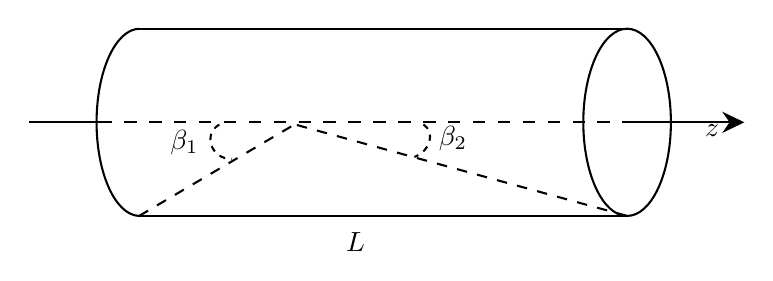
\begin{tikzpicture}[x=0.75pt,y=0.75pt,yscale=-1,xscale=1]
%uncomment if require: \path (0,300); %set diagram left start at 0, and has height of 300

%Shape: Ellipse [id:dp45837335598360185] 
\draw   (400.8,128.9) .. controls (400.8,103.99) and (410.25,83.8) .. (421.9,83.8) .. controls (433.55,83.8) and (443,103.99) .. (443,128.9) .. controls (443,153.81) and (433.55,174) .. (421.9,174) .. controls (410.25,174) and (400.8,153.81) .. (400.8,128.9) -- cycle ;
%Straight Lines [id:da3944094959976163] 
\draw    (186.8,83.8) -- (421.9,83.8) ;
%Straight Lines [id:da2710961804287879] 
\draw    (186.8,174) -- (421.9,174) ;
%Shape: Arc [id:dp5402854435557385] 
\draw  [draw opacity=0] (186.8,174) .. controls (175.44,173.66) and (166.29,153.6) .. (166.29,128.9) .. controls (166.29,104.21) and (175.44,84.15) .. (186.79,83.81) -- (187.09,128.9) -- cycle ; \draw   (186.8,174) .. controls (175.44,173.66) and (166.29,153.6) .. (166.29,128.9) .. controls (166.29,104.21) and (175.44,84.15) .. (186.79,83.81) ;
%Straight Lines [id:da3962843524087052] 
\draw    (421.9,128.9) -- (475.4,128.9) ;
\draw [shift={(478.4,128.9)}, rotate = 180] [fill={rgb, 255:red, 0; green, 0; blue, 0 }  ][line width=0.08]  [draw opacity=0] (10.72,-5.15) -- (0,0) -- (10.72,5.15) -- (7.12,0) -- cycle    ;
%Straight Lines [id:da8460319662973848] 
\draw  [dash pattern={on 4.5pt off 4.5pt}]  (167.6,128.9) -- (421.9,128.9) ;
%Straight Lines [id:da447918090211034] 
\draw    (167.6,128.9) -- (133.6,128.9) ;
%Straight Lines [id:da6481933983683958] 
\draw  [dash pattern={on 3.75pt off 3.75pt on 3.75pt off 3.75pt}]  (186.8,174) -- (261.75,129.9) ;
%Straight Lines [id:da4672537574191007] 
\draw  [dash pattern={on 3.75pt off 3.75pt on 3.75pt off 3.75pt}]  (421.9,174) -- (261.75,129.9) ;
%Curve Lines [id:da5561924047391937] 
\draw  [dash pattern={on 2.25pt off 2.25pt on 2.25pt off 2.25pt}]  (225.4,130) .. controls (217.4,134.6) and (221.4,146.6) .. (231.4,146.6) ;
%Curve Lines [id:da2474593997922261] 
\draw  [dash pattern={on 2.25pt off 2.25pt on 2.25pt off 2.25pt}]  (323.75,129.9) .. controls (329.4,133.6) and (327.4,142.6) .. (319.4,145.6) ;

% Text Node
\draw (458,128.4) node [anchor=north west][inner sep=0.75pt]    {$z$};
% Text Node
\draw (200.4,131.4) node [anchor=north west][inner sep=0.75pt]    {$\beta_{1}$};
% Text Node
\draw (329.75,129.3) node [anchor=north west][inner sep=0.75pt]    {$\beta_{2}$};
% Text Node
\draw (285,180.4) node [anchor=north west][inner sep=0.75pt]    {$L$};


\end{tikzpicture}

            \end{center}
            trong đó: $\left\{ \begin{gathered}
              r = \dfrac{a}{{\sin \beta }} \hfill \\
              z = \dfrac{a}{{\tan \beta }} \hfill \\ 
            \end{gathered}  \right. \Rightarrow \dd z =  - \dfrac{{a \dd\beta }}{{{{\sin }^2}\beta }}$. Do đó, ta có thể viết lại là            \[{\dd}{{{B}}_{z}}=-\dfrac{{{\mu }_{0}}{nI}}{2}\sin \beta {\dd}\beta,\]
            \[ \Rightarrow {{{B}}_{z}}=\dfrac{{{\mu }_{0}}{nI}}{2}\left( \cos {{\beta }_{1}}+\cos {{\beta }_{2}} \right).\]
            Mà ${R} \ll {L}\Rightarrow{{\beta }_{1}}={{\beta }_{2}}\approx 0\Rightarrow {{{B}}_{z}}={{\mu }_{0}}{n}\Rightarrow \overline{{{{H}}_{z}}}={nI}.$\\
            Moment từ của các dòng điện: \[{{\mu }_{{m}}}={nLIS}={nL}\pi {{{R}}^{2}}.\]
            \item Vật liệu hình trụ, bán kính R, ${R} \ll {L}$ xem như ống dây solenoid: \[{B}={{\mu }_{0}}{nI};~{H}={nI}.\]
            Khi thay đổi dòng điện $\dd I$, nguồn điện cần (thực hiện công) chống lại suất điện động cảm ứng xuất hiện trong các vòng dây:
            \[\delta {{{W}}_{0}}=-{{{E}}_{{c}}}{I\dd t},\]
             \[{{{E}}_{{c}}}=-\dfrac{{\dd}\phi }{{\dd t}}.\]
            \[\delta {{{W}}_{0}}=I\dd\phi ={I}\dd \left( {nLB}\pi {{{R}}^{2}} \right)=\left( {L}\pi {{{R}}^{2}} \right){H\dd B},\] trong đó ${B}={{{B}}_{0}}+{{{B}}^{\prime }}={{\mu }_{0}}({H}+{M})$.
            \\Suy ra: 
            \[\delta {{{W}}_{0}}={L}\pi {{{R}}^{2}}\left[ ~{\dd}\left( \dfrac{{{\mu }_{0}}{{{H}}^{2}}}{2} \right)+{{\mu }_{0}}{H \dd M} \right]=\delta {{{W}}_{{ng}}}+\delta {{{W}}_{{m}}}.\]
            Số hạng thứ nhất là biến thiên năng lượng của từ trường ngoài trong không khí, số hạng thứ hai ứng với công mà từ trường ngoài thực hiện đối với khối vật liệu từ. 
        \end{enumerate}
        \item \begin{enumerate}[a)]
            \item Gọi $U$ là nội năng của vật liệu từ. Áp dụng nguyên lí I cho khối vật liệu từ
            \[{dU}=\delta {Q}+\delta {W}={TdS}+{{\mu }_{0}}{L}\pi {{{R}}^{2}}\cdot {H \dd M}. \tag{1} \label{t.1}\]
            Đặt ${G}={U}-{TS}-{{\mu }_{0}}{L}\pi {{{R}}^{2}}{MH}$, có thể thấy $G$ là hàm trạng thái. Lấy vi phân hàm $G$, ta được
            \[{\dd G}={\dd U}-{T\dd S}-{S\dd T}-{{\mu }_{0}}{L}\pi {{{R}}^{2}}\cdot {H\dd M}-{{\mu }_{0}}{L}\pi {{{R}}^{2}}\cdot {M\dd H}. \tag{2} \label{t.2}\]
            Từ (\ref{t.1}) và (\ref{t.2}) suy ra:
            \[{\dd G}=-{S\dd T}-{{\mu }_{0}}{L}\pi {{{R}}^{2}}{M\dd H}. 	\tag{3} \label{t.3}\]
            Từ (\ref{t.3}) suy ra:
            \[\heva{{{S}} =  - {\left. {\dfrac{{\partial {{G}}}}{{\partial {{T}}}}} \right|_{{H}}},\\
              {\mu _0}{{L}}\pi {{{R}}^2} \cdot {{M}} =  - {\left. {\dfrac{{\partial {{G}}}}{{\partial {{H}}}}} \right|_{{T}}} .} \tag{4}\label{t.4}\]
            
            Đạo hàm (\ref{t.4}), ta được: 
            \[\heva{{{\left. \dfrac{\partial {S}}{\partial {H}} \right|}_{{T}}}&=-\dfrac{\partial }{\partial {H}}\left( {{\left. \dfrac{\partial {G}}{\partial {T}} \right|}_{{H}}} \right)=-\dfrac{{{\partial }^{2}}{G}}{\partial {H}\partial {T}},  \\
               {{\left. {{\mu }_{0}}~{L}\pi {{{R}}^{2}}\cdot \dfrac{\partial {M}}{\partial {T}} \right|}_{{H}}}&=-\dfrac{\partial }{\partial {T}}\left( {{\left. \dfrac{\partial {G}}{\partial {H}} \right|}_{{T}}} \right)=-\dfrac{{{\partial }^{2}}{G}}{\partial {T}\partial {H}}.} \tag{5}\label{t.5}\]
            
            Theo (\ref{t.5}) và đề bài, ta suy ra 
            $${{\left. \dfrac{\partial {S}}{\partial {H}} \right|}_{{T}}}={{\left. {{\mu }_{0}}~{L}\pi {{{R}}^{2}}\cdot \dfrac{\partial {M}}{\partial {T}} \right|}_{{H}}};~{{\left. \dfrac{\partial {S}}{\partial {H}} \right|}_{{T}}}={{\left. \alpha \dfrac{\partial {M}}{\partial {T}} \right|}_{{H}}},$$
            \[ \rt  \alpha ={{\mu }_{0}}{L}\pi {{{R}}^{2}}.\]

            \item Ta có: $\delta {Q}={T \dd S};~{{{C}}_{{H}}}={{\left. \dfrac{\delta {Q}}{{dT}} \right|}_{{H}}}={{\left. {T}\dfrac{\partial {S}}{\partial {T}} \right|}_{{H}}}$.
            \\Vì ${S}={S}({T},{H})$ nên một cách tổng quát: \[{\dd S}={{\left. \dfrac{\partial {S}}{\partial {T}} \right|}_{{H}}}{\dd T}+{{\left. \dfrac{\partial {S}}{\partial {H}} \right|}_{{T}}}{\dd H}.\]
            Xét: 
            \[{{\left. \dfrac{\partial {{{C}}_{{H}}}}{\partial {H}} \right|}_{{T}}}={T}\dfrac{\partial }{\partial {H}}\left( {{\left. \dfrac{\partial {S}}{\partial {T}} \right|}_{{H}}} \right)={T}\dfrac{\partial }{\partial {T}}\left( {{\left. \dfrac{\partial S}{\partial {H}} \right|}_{{T}}} \right).\]
            Mặt khác: 
            \[{{\left. \dfrac{\partial {S}}{\partial {H}} \right|}_{{T}}}={{\mu }_{0}}{L}\pi {{{R}}^{2}}\cdot \left. \dfrac{\partial {M}}{\partial {T}}\right|_{H}.\]
            Và lấy đạo hàm phương trình ${M}=\dfrac{{C}}{{T}}{H}$, ta được 
            \[\begin{aligned}
                {{\left. \dfrac{\partial {M}}{\partial {T}} \right|}_{{H}}}&=-\dfrac{{CH}}{{{{T}}^{2}}},\\
                {{\left. \dfrac{\partial {S}}{\partial {H}} \right|}_{{T}}}&={{\left. {{\mu }_{0}}{L}\pi {{{R}}^{2}}\dfrac{\partial {M}}{\partial {T}} \right|}_{{H}}}=-{{\mu }_{0}}{L}\pi {{{R}}^{2}}\dfrac{{CH}}{{{{T}}^{2}}},\\
                \dfrac{\partial }{\partial {T}}\left( {{\left. \dfrac{\partial {S}}{\partial {H}} \right|}_{{T}}} \right)&=2{{\mu }_{0}}{L}\pi {{{R}}^{2}}\dfrac{{CH}}{{{{T}}^{3}}}.
            \end{aligned}\]
            Vậy tìm được: 
            \[\]
            \[\begin{aligned}
            {{\left. \dfrac{\partial {{{C}}_{{H}}}}{\partial {H}} \right|}_{{T}}} &=2{{\mu }_{0}}{L}\pi {{{R}}^{2}}\dfrac{{CH}}{{{{T}}^{2}}},\\
                \Rightarrow {{{C}}_{{H}}} &= \int{2}{{\mu }_{0}}{L}\pi {{{R}}^{2}}\dfrac{{CH}}{{{{T}}^{2}}}{dH} = 2{{\mu }_{0}}{L}\pi {{{R}}^{2}}\dfrac{{C}{{{H}}^{2}}}{~{{{T}}^{2}}}+{C}~({T},{H}=0). \\
                \Rightarrow {{{C}}_{{H}}} &= 2{{\mu }_{0}}~{L}\pi {{{R}}^{2}}\dfrac{{C}{{{H}}^{2}}}{~{{{T}}^{2}}}.
                \end{aligned}\]
                
            
            Tương tự với khí lí tưởng, quá trình đẳng áp: 
            \[{{{C}}_{{p}}}{\dd T}={{{C}}_{{V}}}{\dd T}+{p\dd V}.\] 
            Xét quá trình đẳng từ trường: \[{{{C}}_{{H}}}{\dd T}={{{C}}_{{M}}}{\dd T}+{{\mu }_{0}}{L}\pi {{{R}}^{2}}\cdot {H\dd M}; ~ ({H}\sim{p},{M}\sim{V}).\]
            \[{{{C}}_{{H}}}={{{C}}_{{M}}}+{{\mu }_{0}}~{L}\pi {{{R}}^{2}}{H}\dfrac{{\dd M}}{{\dd T}}.\]
            Mặt khác, theo đề bài, ta có ${M}=\dfrac{{C}}{{T}}{H}$.\\
            Trong quá trình đẳng từ trường (tương tự đẳng áp):
            \[\begin{aligned}
                {\dd M} &=-\dfrac{{CH}}{{{{T}}^{2}}}{\dd}{T},\\
            \Rightarrow \dfrac{{\dd M}}{{\dd T}} & =-\dfrac{{CH}}{{{{T}}^{2}}},\\
            \Rightarrow {{{C}}_{{H}}} &= {{{C}}_{{M}}}-{{\mu }_{0}}{L}\pi {{{R}}^{2}}\dfrac{{C}{{{H}}^{2}}}{~{{{T}}^{2}}},\\
            \Rightarrow {{{C}}_{{M}}} &= 3{{\mu }_{0}}{L}\pi {{{R}}^{2}}\dfrac{{C}{{{H}}^{2}}}{~{{{T}}^{2}}}=3\alpha \dfrac{{{{M}}^{2}}}{{C}}.
            \end{aligned}\]

            \item Ta có: 
            \[{\dd S}={{\left. \dfrac{\partial {S}}{\partial {T}} \right|}_{{H}}}{\dd T}+{{\left. \dfrac{\partial {S}}{\partial {H}} \right|}_{{T}}}{\dd H}.\]
            Với quá trình đoạn nhiệt: \[{\dd S}=0.\]
            Do đó
            \[0=\dfrac{{{{C}}_{{H}}}}{{T}}{\dd T}+{{\mu }_{0}}{L}\pi {{{R}}^{2}}\cdot {{\left. \dfrac{\partial {M}}{\partial {T}} \right|}_{H}}. \tag{6}\label{t.6}\]
            Thay $\dfrac{\partial {M}}{\partial {T}}=-\dfrac{{CH}}{{{{T}}^{2}}};~{  }{{{C}}_{{H}}}=2{{\mu }_{0}}{L}\pi {{{R}}^{2}}\cdot \dfrac{{C}{{{H}}^{2}}}{~{{{T}}^{2}}}$ vào (\ref{t.6}), ta tìm được: 
            \[0=\dfrac{{{\mu }_{0}}{L}\pi {{{R}}^{2}}{C}{{{H}}^{2}}}{~{{{T}}^{3}}}{\dd T}-{{\mu }_{0}}{L}\pi {{{R}}^{2}}\dfrac{{CH}}{{{{T}}^{2}}}{\dd H}.\] 
            Suy ra \[\dfrac{{\dd T}}{{T}}=\dfrac{{\dd H}}{{H}}\Rightarrow \dfrac{{T}}{{H}}= \const.\]

        \end{enumerate}
    \end{enumerate}
\end{loigiai}


\begin{vd}[Lưỡng cực từ và từ trường Trái Đất]
    \begin{enumerate}[1)]
        \item Một dòng điện cường độ $I$ chạy trong vòng dây dẫn tròn bán kính $a$. Chọn hệ toạ độ cầu như hình vẽ, gốc $O$ tại tâm vòng dây. Cảm ứng từ gây ra bởi một phần tử dòng điện $I \dd\ot{a}$ tại điểm có bán kính vector $\ot{r}$ cho bởi công thức Biot - Savart 
        \[\dd\ot{B}=\dfrac{{{\mu }_{0}}}{4\pi }\dfrac{I\dd\ot{a}\times \left( \ot{r}-\ot{a} \right)}{{{\left| \ot{r}-\ot{a} \right|}^{3}}},\] trong đó ${{\mu }_{0}}$ là độ từ thẩm chân không.
        \begin{center}
            

\tikzset{every picture/.style={line width=0.75pt}} %set default line width to 0.75pt        

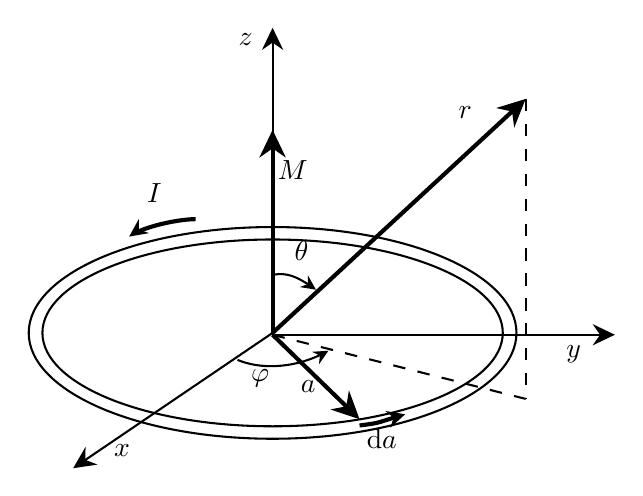
\begin{tikzpicture}[x=0.75pt,y=0.75pt,yscale=-1,xscale=1]
%uncomment if require: \path (0,275); %set diagram left start at 0, and has height of 275

%Curve Lines [id:da10846048595710878] 
\draw [line width=1.5]    (225.28,97.6) .. controls (233.38,93.71) and (246.92,91.2) .. (253.8,91.2) ;
\draw [shift={(221.8,99.6)}, rotate = 324.46] [fill={rgb, 255:red, 0; green, 0; blue, 0 }  ][line width=0.08]  [draw opacity=0] (8.75,-4.2) -- (0,0) -- (8.75,4.2) -- (5.81,0) -- cycle    ;
%Shape: Ellipse [id:dp4359494239874284] 
\draw   (180,146) .. controls (180,121.15) and (229.65,101) .. (290.9,101) .. controls (352.15,101) and (401.8,121.15) .. (401.8,146) .. controls (401.8,170.85) and (352.15,191) .. (290.9,191) .. controls (229.65,191) and (180,170.85) .. (180,146) -- cycle ;
%Shape: Ellipse [id:dp8301142011115972] 
\draw   (173.4,146) .. controls (173.4,117.83) and (226.01,95) .. (290.9,95) .. controls (355.79,95) and (408.4,117.83) .. (408.4,146) .. controls (408.4,174.17) and (355.79,197) .. (290.9,197) .. controls (226.01,197) and (173.4,174.17) .. (173.4,146) -- cycle ;
%Straight Lines [id:da7473886033053341] 
\draw [line width=1.5]    (290.9,52.2) -- (290.9,146) ;
\draw [shift={(290.9,48.2)}, rotate = 90] [fill={rgb, 255:red, 0; green, 0; blue, 0 }  ][line width=0.08]  [draw opacity=0] (13.4,-6.43) -- (0,0) -- (13.4,6.44) -- (8.9,0) -- cycle    ;
%Straight Lines [id:da1050705244766903] 
\draw    (290.9,2) -- (290.9,146.9) ;
\draw [shift={(290.9,-1)}, rotate = 90] [fill={rgb, 255:red, 0; green, 0; blue, 0 }  ][line width=0.08]  [draw opacity=0] (10.72,-5.15) -- (0,0) -- (10.72,5.15) -- (7.12,0) -- cycle    ;
%Straight Lines [id:da8246340112134394] 
\draw [line width=1.5]    (409.86,36.02) -- (290.9,146) ;
\draw [shift={(412.8,33.3)}, rotate = 137.25] [fill={rgb, 255:red, 0; green, 0; blue, 0 }  ][line width=0.08]  [draw opacity=0] (13.4,-6.43) -- (0,0) -- (13.4,6.44) -- (8.9,0) -- cycle    ;
%Straight Lines [id:da045367212215944974] 
\draw    (452.8,146.9) -- (290.9,146.9) ;
\draw [shift={(455.8,146.9)}, rotate = 180] [fill={rgb, 255:red, 0; green, 0; blue, 0 }  ][line width=0.08]  [draw opacity=0] (10.72,-5.15) -- (0,0) -- (10.72,5.15) -- (7.12,0) -- cycle    ;
%Straight Lines [id:da44434161916099746] 
\draw    (197.28,209.52) -- (290.9,146) ;
\draw [shift={(194.8,211.2)}, rotate = 325.84] [fill={rgb, 255:red, 0; green, 0; blue, 0 }  ][line width=0.08]  [draw opacity=0] (10.72,-5.15) -- (0,0) -- (10.72,5.15) -- (7.12,0) -- cycle    ;
%Curve Lines [id:da45261085476343466] 
\draw [line width=1.5]    (332.8,190.6) .. controls (342.75,189.33) and (340.42,189.54) .. (351.01,186.33) ;
\draw [shift={(354.8,185.2)}, rotate = 523.65] [fill={rgb, 255:red, 0; green, 0; blue, 0 }  ][line width=0.08]  [draw opacity=0] (8.75,-4.2) -- (0,0) -- (8.75,4.2) -- (5.81,0) -- cycle    ;
%Straight Lines [id:da25789478426205514] 
\draw  [dash pattern={on 4.5pt off 4.5pt}]  (412.8,33.3) -- (412.8,177.8) ;
%Straight Lines [id:da0983954858588747] 
\draw  [dash pattern={on 4.5pt off 4.5pt}]  (290.9,146.9) -- (412.8,177.8) ;
%Curve Lines [id:da03253666468920291] 
\draw    (291,118) .. controls (297.98,116.75) and (302.72,119.02) .. (309.37,123.52) ;
\draw [shift={(311.8,125.2)}, rotate = 214.99] [fill={rgb, 255:red, 0; green, 0; blue, 0 }  ][line width=0.08]  [draw opacity=0] (7.14,-3.43) -- (0,0) -- (7.14,3.43) -- (4.74,0) -- cycle    ;
%Curve Lines [id:da06311953128296643] 
\draw    (274,159) .. controls (284.21,163.35) and (299.95,163.59) .. (315.15,156) ;
\draw [shift={(317.8,154.6)}, rotate = 510.64] [fill={rgb, 255:red, 0; green, 0; blue, 0 }  ][line width=0.08]  [draw opacity=0] (7.14,-3.43) -- (0,0) -- (7.14,3.43) -- (4.74,0) -- cycle    ;
%Straight Lines [id:da8985736362886838] 
\draw [line width=1.5]    (329.93,184.81) -- (290.9,146.9) ;
\draw [shift={(332.8,187.6)}, rotate = 224.17] [fill={rgb, 255:red, 0; green, 0; blue, 0 }  ][line width=0.08]  [draw opacity=0] (13.4,-6.43) -- (0,0) -- (13.4,6.44) -- (8.9,0) -- cycle    ;


% Text Node
\draw (229,72.4) node [anchor=north west][inner sep=0.75pt]    {$I$};
% Text Node
\draw (303,167.4) node [anchor=north west][inner sep=0.75pt]    {$\ot{a}$};
% Text Node
\draw (334.8,191) node [anchor=north west][inner sep=0.75pt]    {$\mathrm{d}\ot{a}$};
% Text Node
\draw (213,198.4) node [anchor=north west][inner sep=0.75pt]    {$x$};
% Text Node
\draw (431,150.4) node [anchor=north west][inner sep=0.75pt]    {$y$};
% Text Node
\draw (273,0.4) node [anchor=north west][inner sep=0.75pt]    {$z$};
% Text Node
\draw (292,61.4) node [anchor=north west][inner sep=0.75pt]    {$\ot{M}$};
% Text Node
\draw (379,35.4) node [anchor=north west][inner sep=0.75pt]    {$\ot{r}$};
% Text Node
\draw (279,162.4) node [anchor=north west][inner sep=0.75pt]    {$\varphi $};
% Text Node
\draw (300,100.4) node [anchor=north west][inner sep=0.75pt]    {$\theta $};


\end{tikzpicture}

        \end{center}
        \begin{enumerate}[a)]
            \item Chứng tỏ rằng từ trường do vòng dây tạo ra tại những điểm cách xa tâm vòng dây $\left( \left| {\ot{r}} \right| \gg a \right)$ có thể biểu diễn gần đúng dưới dạng \[\ot{B}=\dfrac{{{\mu }_{0}}}{4\pi }\left[ \dfrac{3\left( \overrightarrow{M}.\ot{r} \right)\ot{r}}{{{r}^{5}}}-\dfrac{\overrightarrow{M}}{{{r}^{3}}} \right],\] trong đó $\di \overrightarrow{M}=\dfrac{1}{2}I\oint{\ot{a}\times \dd\ot{a}}$ là moment từ của vòng dây.
            \item Các đường sức từ nằm trong một mặt phẳng chứa trục $Oz$ có phương trình dạng $r=r\left( \theta  \right)$. Phân tích vector cảm ứng từ thành hai thành phần ${{\ot{B_{r}}}}$ và ${{\ot{B_{\theta }}}}$ (Hình vẽ). Viết biểu thức của ${{B}_{r}}$, ${{B}_{\theta }}$ và phương trình $r=r\left( \theta  \right)$.
            \begin{center}
                

\tikzset{every picture/.style={line width=0.75pt}} %set default line width to 0.75pt        

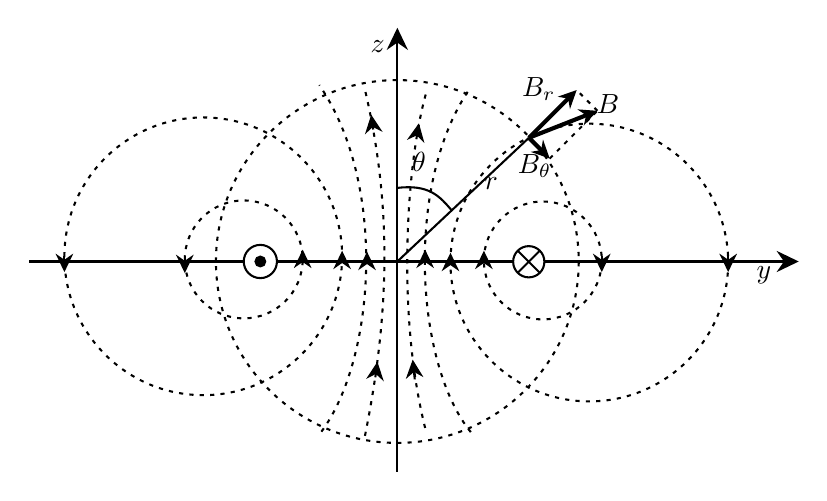
\begin{tikzpicture}[x=0.75pt,y=0.75pt,yscale=-1,xscale=1]
%uncomment if require: \path (0,556); %set diagram left start at 0, and has height of 556

%Shape: Circle [id:dp29085209309514837] 
\draw  [dash pattern={on 1.5pt off 2.25pt on 1.5pt off 2.25pt}] (127,155.9) .. controls (127,118.95) and (156.95,89) .. (193.9,89) .. controls (230.85,89) and (260.8,118.95) .. (260.8,155.9) .. controls (260.8,192.85) and (230.85,222.8) .. (193.9,222.8) .. controls (156.95,222.8) and (127,192.85) .. (127,155.9) -- cycle ;
%Shape: Circle [id:dp02434157926950764] 
\draw  [dash pattern={on 1.5pt off 2.25pt on 1.5pt off 2.25pt}] (185,157.4) .. controls (185,141.72) and (197.72,129) .. (213.4,129) .. controls (229.08,129) and (241.8,141.72) .. (241.8,157.4) .. controls (241.8,173.08) and (229.08,185.8) .. (213.4,185.8) .. controls (197.72,185.8) and (185,173.08) .. (185,157.4) -- cycle ;
%Shape: Circle [id:dp8524046644913632] 
\draw  [dash pattern={on 1.5pt off 2.25pt on 1.5pt off 2.25pt}] (200,158.4) .. controls (200,110.13) and (239.13,71) .. (287.4,71) .. controls (335.67,71) and (374.8,110.13) .. (374.8,158.4) .. controls (374.8,206.67) and (335.67,245.8) .. (287.4,245.8) .. controls (239.13,245.8) and (200,206.67) .. (200,158.4) -- cycle ;
%Shape: Circle [id:dp9411045521853414] 
\draw  [dash pattern={on 1.5pt off 2.25pt on 1.5pt off 2.25pt}] (313,158.9) .. controls (313,121.95) and (342.95,92) .. (379.9,92) .. controls (416.85,92) and (446.8,121.95) .. (446.8,158.9) .. controls (446.8,195.85) and (416.85,225.8) .. (379.9,225.8) .. controls (342.95,225.8) and (313,195.85) .. (313,158.9) -- cycle ;
%Shape: Circle [id:dp10858406922344166] 
\draw  [dash pattern={on 1.5pt off 2.25pt on 1.5pt off 2.25pt}] (329.1,157.9) .. controls (329.1,142.22) and (341.82,129.5) .. (357.5,129.5) .. controls (373.18,129.5) and (385.9,142.22) .. (385.9,157.9) .. controls (385.9,173.58) and (373.18,186.3) .. (357.5,186.3) .. controls (341.82,186.3) and (329.1,173.58) .. (329.1,157.9) -- cycle ;
%Curve Lines [id:da2835143374759419] 
\draw  [dash pattern={on 1.5pt off 2.25pt on 1.5pt off 2.25pt}]  (250.8,240.4) .. controls (276.6,205.8) and (282.8,121.4) .. (249.8,73.4) ;
%Curve Lines [id:da4647059616083795] 
\draw  [dash pattern={on 1.5pt off 2.25pt on 1.5pt off 2.25pt}]  (271.8,242.4) .. controls (283.8,182.6) and (284.8,131.6) .. (271.8,75.6) ;
%Curve Lines [id:da6822020489603986] 
\draw  [dash pattern={on 1.5pt off 2.25pt on 1.5pt off 2.25pt}]  (322.8,240.6) .. controls (295.8,207.6) and (290.8,119.6) .. (322.8,74.4) ;
%Curve Lines [id:da23486398367518735] 
\draw  [dash pattern={on 1.5pt off 2.25pt on 1.5pt off 2.25pt}]  (300.8,238.6) .. controls (286.8,182.6) and (291.8,108.6) .. (301.8,75.4) ;
%Straight Lines [id:da6581838405585771] 
\draw    (477.8,158.4) -- (109.8,158.4) ;
\draw [shift={(480.8,158.4)}, rotate = 180] [fill={rgb, 255:red, 0; green, 0; blue, 0 }  ][line width=0.08]  [draw opacity=0] (10.72,-5.15) -- (0,0) -- (10.72,5.15) -- (7.12,0) -- cycle    ;
%Straight Lines [id:da22556909074791687] 
\draw    (287.4,259.8) -- (287.4,48.8) ;
\draw [shift={(287.4,45.8)}, rotate = 450] [fill={rgb, 255:red, 0; green, 0; blue, 0 }  ][line width=0.08]  [draw opacity=0] (10.72,-5.15) -- (0,0) -- (10.72,5.15) -- (7.12,0) -- cycle    ;
%Straight Lines [id:da71492483037083] 
\draw    (287.4,158.4) -- (350.8,98.8) ;
%Straight Lines [id:da7508025535197118] 
\draw [line width=1.5]    (350.8,98.8) -- (370.97,78.63) ;
\draw [shift={(373.8,75.8)}, rotate = 495] [fill={rgb, 255:red, 0; green, 0; blue, 0 }  ][line width=0.08]  [draw opacity=0] (8.75,-4.2) -- (0,0) -- (8.75,4.2) -- (5.81,0) -- cycle    ;
%Straight Lines [id:da9592755449173642] 
\draw [line width=1.5]    (350.8,98.8) -- (357.97,105.97) ;
\draw [shift={(360.8,108.8)}, rotate = 225] [fill={rgb, 255:red, 0; green, 0; blue, 0 }  ][line width=0.08]  [draw opacity=0] (8.75,-4.2) -- (0,0) -- (8.75,4.2) -- (5.81,0) -- cycle    ;
%Straight Lines [id:da26223212039294874] 
\draw [line width=1.5]    (350.8,98.8) -- (380.08,87.27) ;
\draw [shift={(383.8,85.8)}, rotate = 518.5] [fill={rgb, 255:red, 0; green, 0; blue, 0 }  ][line width=0.08]  [draw opacity=0] (8.75,-4.2) -- (0,0) -- (8.75,4.2) -- (5.81,0) -- cycle    ;
%Straight Lines [id:da39606688350301766] 
\draw  [dash pattern={on 1.5pt off 2.25pt on 1.5pt off 2.25pt}]  (383.8,85.8) -- (373.8,75.8) ;
%Straight Lines [id:da26627580934964135] 
\draw  [dash pattern={on 1.5pt off 2.25pt on 1.5pt off 2.25pt}]  (360.8,108.8) -- (383.8,85.8) ;
%Flowchart: Connector [id:dp813336365610398] 
\draw  [fill={rgb, 255:red, 255; green, 255; blue, 255 }  ,fill opacity=1 ] (213.4,158.4) .. controls (213.4,153.98) and (216.98,150.4) .. (221.4,150.4) .. controls (225.82,150.4) and (229.4,153.98) .. (229.4,158.4) .. controls (229.4,162.82) and (225.82,166.4) .. (221.4,166.4) .. controls (216.98,166.4) and (213.4,162.82) .. (213.4,158.4) -- cycle ;
%Flowchart: Connector [id:dp13819250068029332] 
\draw  [fill={rgb, 255:red, 0; green, 0; blue, 0 }  ,fill opacity=1 ] (219.05,158.4) .. controls (219.05,157.1) and (220.1,156.05) .. (221.4,156.05) .. controls (222.7,156.05) and (223.75,157.1) .. (223.75,158.4) .. controls (223.75,159.7) and (222.7,160.75) .. (221.4,160.75) .. controls (220.1,160.75) and (219.05,159.7) .. (219.05,158.4) -- cycle ;
%Flowchart: Summing Junction [id:dp9094327816396024] 
\draw  [fill={rgb, 255:red, 255; green, 255; blue, 255 }  ,fill opacity=1 ] (343.2,158.52) .. controls (343.2,154.37) and (346.57,151) .. (350.73,151) .. controls (354.88,151) and (358.25,154.37) .. (358.25,158.52) .. controls (358.25,162.68) and (354.88,166.05) .. (350.73,166.05) .. controls (346.57,166.05) and (343.2,162.68) .. (343.2,158.52) -- cycle ; \draw   (345.4,153.2) -- (356.05,163.85) ; \draw   (356.05,153.2) -- (345.4,163.85) ;
%Straight Lines [id:da24348604208625568] 
\draw    (127,155.9) -- (127,160.5) ;
\draw [shift={(127,163.5)}, rotate = 270] [fill={rgb, 255:red, 0; green, 0; blue, 0 }  ][line width=0.08]  [draw opacity=0] (8.93,-4.29) -- (0,0) -- (8.93,4.29) -- (5.93,0) -- cycle    ;
%Straight Lines [id:da06446323079089988] 
\draw    (185,156.4) -- (185,161) ;
\draw [shift={(185,164)}, rotate = 270] [fill={rgb, 255:red, 0; green, 0; blue, 0 }  ][line width=0.08]  [draw opacity=0] (8.93,-4.29) -- (0,0) -- (8.93,4.29) -- (5.93,0) -- cycle    ;
%Straight Lines [id:da19623197471427423] 
\draw    (385.9,155.9) -- (385.9,160.5) ;
\draw [shift={(385.9,163.5)}, rotate = 270] [fill={rgb, 255:red, 0; green, 0; blue, 0 }  ][line width=0.08]  [draw opacity=0] (8.93,-4.29) -- (0,0) -- (8.93,4.29) -- (5.93,0) -- cycle    ;
%Straight Lines [id:da5057241487299509] 
\draw    (446.8,155.9) -- (446.8,160.5) ;
\draw [shift={(446.8,163.5)}, rotate = 270] [fill={rgb, 255:red, 0; green, 0; blue, 0 }  ][line width=0.08]  [draw opacity=0] (8.93,-4.29) -- (0,0) -- (8.93,4.29) -- (5.93,0) -- cycle    ;
%Straight Lines [id:da7593898108105328] 
\draw    (241.8,158.4) -- (241.8,155.7) ;
\draw [shift={(241.8,152.7)}, rotate = 450] [fill={rgb, 255:red, 0; green, 0; blue, 0 }  ][line width=0.08]  [draw opacity=0] (8.93,-4.29) -- (0,0) -- (8.93,4.29) -- (5.93,0) -- cycle    ;
%Straight Lines [id:da813195177932039] 
\draw    (260.8,158.9) -- (260.8,156.2) ;
\draw [shift={(260.8,153.2)}, rotate = 450] [fill={rgb, 255:red, 0; green, 0; blue, 0 }  ][line width=0.08]  [draw opacity=0] (8.93,-4.29) -- (0,0) -- (8.93,4.29) -- (5.93,0) -- cycle    ;
%Straight Lines [id:da7008691584468463] 
\draw    (272.8,159.4) -- (272.8,156.7) ;
\draw [shift={(272.8,153.7)}, rotate = 450] [fill={rgb, 255:red, 0; green, 0; blue, 0 }  ][line width=0.08]  [draw opacity=0] (8.93,-4.29) -- (0,0) -- (8.93,4.29) -- (5.93,0) -- cycle    ;
%Straight Lines [id:da31890931115343] 
\draw    (276.8,214.2) -- (277.4,209.67) ;
\draw [shift={(277.8,206.7)}, rotate = 457.59] [fill={rgb, 255:red, 0; green, 0; blue, 0 }  ][line width=0.08]  [draw opacity=0] (8.93,-4.29) -- (0,0) -- (8.93,4.29) -- (5.93,0) -- cycle    ;
%Straight Lines [id:da6049143635099812] 
\draw    (295.8,215.2) -- (295.11,208.68) ;
\draw [shift={(294.8,205.7)}, rotate = 443.99] [fill={rgb, 255:red, 0; green, 0; blue, 0 }  ][line width=0.08]  [draw opacity=0] (8.93,-4.29) -- (0,0) -- (8.93,4.29) -- (5.93,0) -- cycle    ;
%Straight Lines [id:da8757833444043637] 
\draw    (300.8,158.4) -- (300.8,155.7) ;
\draw [shift={(300.8,152.7)}, rotate = 450] [fill={rgb, 255:red, 0; green, 0; blue, 0 }  ][line width=0.08]  [draw opacity=0] (8.93,-4.29) -- (0,0) -- (8.93,4.29) -- (5.93,0) -- cycle    ;
%Straight Lines [id:da30601086688417567] 
\draw    (313,159.9) -- (313,157.2) ;
\draw [shift={(313,154.2)}, rotate = 450] [fill={rgb, 255:red, 0; green, 0; blue, 0 }  ][line width=0.08]  [draw opacity=0] (8.93,-4.29) -- (0,0) -- (8.93,4.29) -- (5.93,0) -- cycle    ;
%Straight Lines [id:da2455636936810508] 
\draw    (329.1,158.9) -- (329.1,156.2) ;
\draw [shift={(329.1,153.2)}, rotate = 450] [fill={rgb, 255:red, 0; green, 0; blue, 0 }  ][line width=0.08]  [draw opacity=0] (8.93,-4.29) -- (0,0) -- (8.93,4.29) -- (5.93,0) -- cycle    ;
%Straight Lines [id:da3391481816537072] 
\draw    (296.8,97.4) -- (297.27,94.75) ;
\draw [shift={(297.8,91.8)}, rotate = 460.12] [fill={rgb, 255:red, 0; green, 0; blue, 0 }  ][line width=0.08]  [draw opacity=0] (8.93,-4.29) -- (0,0) -- (8.93,4.29) -- (5.93,0) -- cycle    ;
%Straight Lines [id:da2058542206609797] 
\draw    (275.8,94.8) -- (275.22,90.67) ;
\draw [shift={(274.8,87.7)}, rotate = 441.98] [fill={rgb, 255:red, 0; green, 0; blue, 0 }  ][line width=0.08]  [draw opacity=0] (8.93,-4.29) -- (0,0) -- (8.93,4.29) -- (5.93,0) -- cycle    ;
%Curve Lines [id:da1147654647970966] 
\draw    (287,123) .. controls (302.8,121) and (307.8,127) .. (313.8,134) ;


% Text Node
\draw (293,104.4) node [anchor=north west][inner sep=0.75pt]    {$\theta $};
% Text Node
\draw (328,116.4) node [anchor=north west][inner sep=0.75pt]    {$r$};
% Text Node
\draw (346,68.4) node [anchor=north west][inner sep=0.75pt]    {$B_{r}$};
% Text Node
\draw (344,105.4) node [anchor=north west][inner sep=0.75pt]    {$B_{\theta }$};
% Text Node
\draw (382,76.4) node [anchor=north west][inner sep=0.75pt]    {$B$};
% Text Node
\draw (273,50.4) node [anchor=north west][inner sep=0.75pt]    {$z$};
% Text Node
\draw (459,159.4) node [anchor=north west][inner sep=0.75pt]    {$y$};


\end{tikzpicture}

            \end{center}
        \end{enumerate}
        \item Coi từ trường Trái Đất giống như ý $1)$. Ta sử dụng hệ toạ độ cầu mà mặt phẳng xích đạo vuông góc với moment từ (gọi là mặt phẳng xích đạo từ, nghiêng $11^{\circ}$ so với mặt phẳng xích đạo địa lí).
        Khi các hạt mang điện bay từ vũ trụ đến Trái Đất, tuỳ thuộc vào hướng và độ lớn của vận tốc, chúng có thể xuyên qua, hoặc bị phản xạ bay ngược lại hoặc bị giam giữ trong từ trường này. Coi hệ quy chiếu gắn với Trái Đất là quán tính, bỏ qua chuyển động tự quay của Trái Đất và trọng trường của nó.
    \begin{enumerate}[a)]
        \item Chứng tỏ rằng khi một hạt khối lượng $m$, điện tích $q$ chuyển động trong từ trường thì đại lượng ${{\sin }^{2}}\theta \left( m{{r}^{2}}\dfrac{\dd \varphi }{\dd t}+\dfrac{{{\mu }_{0}}}{4\pi }\dfrac{qM}{r} \right)$ được bảo toàn.
        \item Xét hạt ở xa vô cùng chuyển động đến Trái Đất với vận tốc $v$ nằm trong mặt phẳng xích đạo từ $\left( \theta =\pi /2 \right)$. Gọi $b$ là khoảng cách từ tâm Trái Đất đến phương ban đầu của vận tốc. Tìm khoảng cách cực tiểu từ hạt tới tâm Trái Đất.
    \end{enumerate}
    \item Nếu vận tốc ban đầu của hạt không nằm trong mặt phẳng xích đạo từ, chuyển động của nó rất phức tạp nhưng ta sẽ mô tả nó đơn giản hơn bằng một số phép gần đúng. Xét trường hợp các hạt bị giam giữ trong từ trường của Trái Đất. Chuyển động của hạt có thể phân tích thành $3$ chuyển động thành phần với các chu kì ${{\tau }_{1}},\,{{\tau }_{2}},\,{{\tau }_{3}}$ tương ứng $({{\tau }_{3}}\gg{{\tau }_{2}}\gg{{\tau }_{1}})$.
    \begin{itemize}
        \item Chuyển động quay trên một quỹ đạo tròn vuông góc với đường sức từ.
        \item Chuyển động trượt dọc theo đường sức từ
        (Hai chuyển động trên tạo thành chuyển động xoắn ốc trong mặt phẳng kinh tuyến cố định như trên hình vẽ).
        \begin{center}
            

\tikzset{every picture/.style={line width=0.75pt}} %set default line width to 0.75pt        

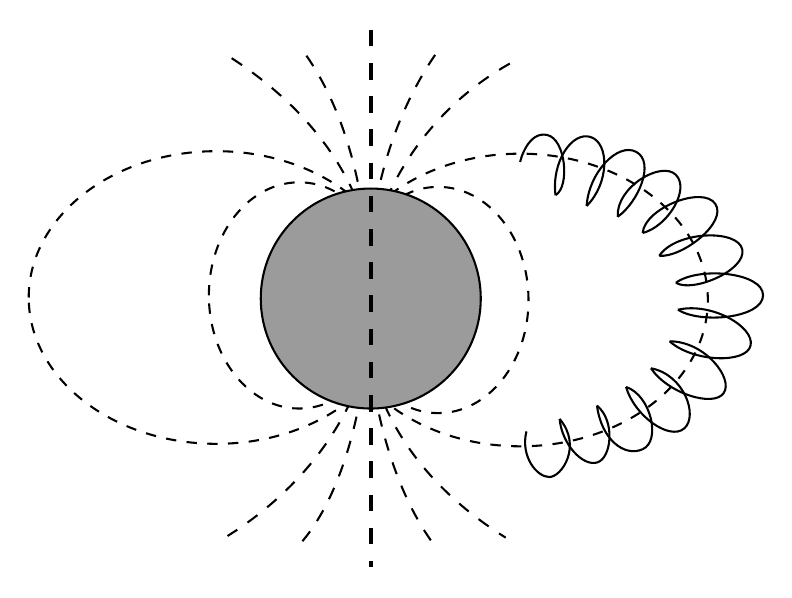
\begin{tikzpicture}[x=0.75pt,y=0.75pt,yscale=-1,xscale=1]
%uncomment if require: \path (0,300); %set diagram left start at 0, and has height of 300

%Curve Lines [id:da6132579702161214] 
\draw  [dash pattern={on 4.5pt off 4.5pt}]  (222.8,47.2) .. controls (323.8,113) and (306.8,223.4) .. (220.8,277.4) ;
%Curve Lines [id:da02753651947126423] 
\draw  [dash pattern={on 4.5pt off 4.5pt}]  (356.8,49.8) .. controls (277.8,94) and (249.8,212.6) .. (354.8,278.2) ;
%Curve Lines [id:da45357572284251124] 
\draw  [dash pattern={on 4.5pt off 4.5pt}]  (320.8,45.6) .. controls (316.65,51.68) and (312.94,58.04) .. (309.63,64.62) .. controls (273.84,135.79) and (285.85,232.92) .. (318.8,279.6) ;
%Curve Lines [id:da8654207804304774] 
\draw  [dash pattern={on 4.5pt off 4.5pt}]  (258.8,46) .. controls (303.8,110.8) and (294.8,235) .. (256.8,280) ;
%Curve Lines [id:da38926372407720966] 
\draw    (361.8,97.2) .. controls (361.8,96.2) and (365.8,82.2) .. (374.8,84.2) .. controls (383.8,86.2) and (385.8,109.2) .. (378.8,113.2) ;
%Curve Lines [id:da2139253061785582] 
\draw    (378.8,113.2) .. controls (376.8,97.2) and (386.8,82.2) .. (395.8,85.2) .. controls (404.8,88.2) and (404.8,107.4) .. (393.8,118.4) ;
%Curve Lines [id:da4547475730350532] 
\draw    (393.8,118.4) .. controls (394.8,102.4) and (408.8,87.4) .. (417.8,92.4) .. controls (426.8,97.4) and (418.8,116.4) .. (408.8,123.6) ;
%Curve Lines [id:da23447614846936116] 
\draw    (408.8,123.6) .. controls (407.8,109.4) and (429.8,96.4) .. (436.8,103.4) .. controls (443.8,110.4) and (432.8,128.4) .. (420.8,131.4) ;
%Curve Lines [id:da55567583729151] 
\draw    (420.8,131.4) .. controls (421.8,119.4) and (449.8,108.4) .. (455.8,117.4) .. controls (461.8,126.4) and (439.8,143.4) .. (428.8,142.4) ;
%Curve Lines [id:da08531518632852353] 
\draw    (428.8,142.4) .. controls (436.8,130.4) and (466.8,129.4) .. (468.8,139.4) .. controls (470.8,149.4) and (444.8,160.4) .. (436.8,155.4) ;
%Curve Lines [id:da7887996819217282] 
\draw    (436.8,155.4) .. controls (447.8,147.4) and (478.8,150.4) .. (478.8,161.4) .. controls (478.8,172.4) and (448.8,175.4) .. (437.8,168.4) ;
%Curve Lines [id:da7015116734835025] 
\draw    (437.8,168.4) .. controls (453.8,164.6) and (474.8,176.6) .. (472.8,185.6) .. controls (470.8,194.6) and (444.8,193.6) .. (433.8,183.6) ;
%Curve Lines [id:da7242135718091796] 
\draw    (433.8,183.6) .. controls (450.8,183.6) and (464.8,201.6) .. (459.8,208.6) .. controls (454.8,215.6) and (432.8,208.6) .. (424.8,196.6) ;
%Curve Lines [id:da9262604601374971] 
\draw    (424.8,196.6) .. controls (440.8,199.6) and (447.8,219.6) .. (440.8,225.6) .. controls (433.8,231.6) and (416.8,219.6) .. (412.8,205.6) ;
%Curve Lines [id:da35076738041725486] 
\draw    (412.8,205.6) .. controls (424.8,209.6) and (429.8,231.6) .. (420.8,235.6) .. controls (411.8,239.6) and (400.8,230.6) .. (398.8,214.6) ;
%Curve Lines [id:da9971771592169689] 
\draw    (398.8,214.6) .. controls (407.8,222) and (405.8,240) .. (398.8,242) .. controls (391.8,244) and (381.8,233) .. (380.8,221) ;
%Curve Lines [id:da34941232204370487] 
\draw    (380.8,221) .. controls (391.8,234) and (381.8,249) .. (375.8,249) .. controls (369.8,249) and (361.8,239) .. (364.8,227) ;
%Shape: Ellipse [id:dp7720112072252094] 
\draw  [dash pattern={on 3.75pt off 3.75pt on 3.75pt off 3.75pt}] (125,162.5) .. controls (125,123.56) and (165.47,92) .. (215.4,92) .. controls (265.33,92) and (305.8,123.56) .. (305.8,162.5) .. controls (305.8,201.44) and (265.33,233) .. (215.4,233) .. controls (165.47,233) and (125,201.44) .. (125,162.5) -- cycle ;
%Shape: Ellipse [id:dp2433695358279957] 
\draw  [dash pattern={on 3.75pt off 3.75pt on 3.75pt off 3.75pt}] (271.4,163.7) .. controls (271.4,124.76) and (311.87,93.2) .. (361.8,93.2) .. controls (411.73,93.2) and (452.2,124.76) .. (452.2,163.7) .. controls (452.2,202.64) and (411.73,234.2) .. (361.8,234.2) .. controls (311.87,234.2) and (271.4,202.64) .. (271.4,163.7) -- cycle ;
%Shape: Ellipse [id:dp7240270686858918] 
\draw  [dash pattern={on 3.75pt off 3.75pt on 3.75pt off 3.75pt}] (211.8,161.5) .. controls (211.8,131.4) and (231.28,107) .. (255.3,107) .. controls (279.32,107) and (298.8,131.4) .. (298.8,161.5) .. controls (298.8,191.6) and (279.32,216) .. (255.3,216) .. controls (231.28,216) and (211.8,191.6) .. (211.8,161.5) -- cycle ;
%Shape: Ellipse [id:dp1354173556714764] 
\draw  [dash pattern={on 3.75pt off 3.75pt on 3.75pt off 3.75pt}] (278.8,163.7) .. controls (278.8,133.6) and (298.28,109.2) .. (322.3,109.2) .. controls (346.32,109.2) and (365.8,133.6) .. (365.8,163.7) .. controls (365.8,193.8) and (346.32,218.2) .. (322.3,218.2) .. controls (298.28,218.2) and (278.8,193.8) .. (278.8,163.7) -- cycle ;
%Shape: Circle [id:dp44270730118622503] 
\draw  [fill={rgb, 255:red, 155; green, 155; blue, 155 }  ,fill opacity=1 ] (236.8,163) .. controls (236.8,133.73) and (260.53,110) .. (289.8,110) .. controls (319.07,110) and (342.8,133.73) .. (342.8,163) .. controls (342.8,192.27) and (319.07,216) .. (289.8,216) .. controls (260.53,216) and (236.8,192.27) .. (236.8,163) -- cycle ;
%Straight Lines [id:da40622260608131233] 
\draw [line width=1.5]  [dash pattern={on 6pt off 6pt on 6pt off 6pt}]  (289.8,33.5) -- (289.8,292.5) ;





\end{tikzpicture}

        \end{center}
        \item Chuyển động quay của mặt phẳng kinh tuyến xung quanh trục moment từ.
    \end{itemize}
        \begin{enumerate}[a)]
            \item Nếu bán kính chuyển động tròn đủ nhỏ, ta có thể coi từ trường là đều. Phân tích vận tốc $\ot{v}$ của hạt thành hai thành phần vuông góc ${{\ot{v_{\perp}}}}$ và song song ${{\ot{v_{\parallel}}}}$ với từ trường. Tìm biểu thức của bán kính và tần số góc của hạt theo $m,\,q,\,B,\,{{v}_{\perp }}$.
            \item Khi tâm quay của hạt chuyển động dọc theo đường sức từ, từ trường có độ lớn thay đổi. Trong hệ quy chiếu gắn với tâm quay, từ trường biến thiên theo thời gian. Chỉ ra rằng nếu từ trường biến thiên đủ chậm thì từ thông gửi qua diện tích chắn bởi quỹ đạo quay của hạt là hằng số, từ đó suy ra moment từ trong chuyển động tròn của hạt là hằng số.
            \item Khi lại gần hai cực, từ trường mạnh lên, bán kính quay giảm, do vậy vận tốc ${{v}_{\perp }}$ tăng lên. Bảo toàn năng lượng đòi hỏi vận tốc trượt ${{v}_{\parallel}}$ giảm. Tại điểm mà ${{v}_{\parallel}}=0$ thì hạt ngừng trượt và sau đó trượt ngược lại, điểm này gọi là điểm gương. Tìm biểu thức xác định vị trí điểm gương theo giá trị góc ${{\alpha }_{0}}$ là góc tạo bởi phương chuyển động của hạt và đường sức từ khi hạt chuyển động cắt mặt phẳng xích đạo từ.
            \item Tìm biểu thức tính chu kì trượt ${{\tau }_{2}}$ theo $v,\,{{\alpha }_{0}}$ và khoảng cách ${{R}_{0}}$ từ hạt tới tâm Trái Đất tại mặt phẳng xích đạo.
            \item Tìm chu kì quay ${{\tau }_{3}}$ của mặt phẳng kinh tuyến xung quanh trục moment từ.
        \end{enumerate}
    \end{enumerate}
    Cho:
    \begin{itemize}
        \item Phép gần đúng \[\dfrac{1}{{{\left| \ot{r}-\ot{a} \right|}^{3}}}\approx \dfrac{1}{{{r}^{3}}}+\dfrac{3\ot{r}.\ot{a}}{{{r}^{5}}} \ \text{ khi } \ r\gg a.\]
        \item Các thành phần của vector vận tốc trong toạ độ cầu $\left( {{v}_{r}},{{v}_{\theta }},{{v}_{\varphi }} \right)=\left( \dfrac{\dd r}{\dd t},r\dfrac{\dd\theta }{\dd t},r\sin \theta \dfrac{\dd\varphi }{\dd t} \right)$.
    \end{itemize}
\end{vd}
\begin{loigiai}
    \begin{enumerate}[1)]
        \item Từ trường thu được bằng cách tích phân dọc theo vòng dây 
        \[\ot{B}=\oint{\dfrac{{{\mu }_{0}}}{4\pi }.\dfrac{Id\ot{a}\times \left( \ot{r}-\ot{a} \right)}{{{\left| \ot{r}-\ot{a} \right|}^{3}}}}.\]
        \begin{enumerate}[a)]
            \item Tại những điểm cách xa tâm vòng dây $r \gg a$ ta khai triển 
            \[\dfrac{1}{{{\left| \ot{r}-\ot{a} \right|}^{3}}}\approx \dfrac{1}{{{r}^{3}}}+\dfrac{3\ot{r}.\ot{a}}{{{r}^{5}}}.\]
            Thế vào tích phân trên, ta được
            \[\ot{B}=\dfrac{{{\mu }_{0}}I}{4\pi }\left[ \oint{\dfrac{\dd\ot{a}\times \ot{r}}{{{r}^{3}}}}-\oint{\dfrac{\dd\ot{a}\times \ot{a}}{{{r}^{3}}}}+\oint{\dfrac{3\ot{r}.\ot{a}}{{{r}^{5}}}\dd\ot{a}\times \ot{r}}-\oint{\dfrac{3\ot{r}.\ot{a}}{{{r}^{5}}}\dd\ot{a}\times \ot{a}} \right].\]
            Tích phân thứ nhất bằng không cho một đường cong kín bất kì. Tích phân thứ hai và thứ ba sau khi lấy sẽ tỉ lệ với $\dfrac{1}{{{r}^{3}}}$, còn tích phân cuối tỉ lệ với $\dfrac{1}{{{r}^{4}}}$ nên có thể bỏ qua.\\
            Còn lại 
            \[\begin{aligned}
                \ot{B}&=\dfrac{{{\mu }_{0}}I}{4\pi }\left[ -\oint{\dfrac{\dd\ot{a}\times \ot{a}}{{{r}^{3}}}}+\oint{\dfrac{3\ot{r}.\ot{a}}{{{r}^{5}}}\dd\ot{a}\times \ot{r}} \right]\\
                &=\dfrac{{{\mu }_{0}}I}{4\pi }\left\{ \dfrac{1}{{{r}^{3}}}\oint{\ot{a}\times \dd\ot{a}}+\dfrac{3}{{{r}^{5}}}\left[ \oint{\left( \ot{r}.\ot{a} \right)\dd\ot{a}} \right]\times \ot{r} \right\}.
            \end{aligned} \]
            \[\oint{\left( \ot{r}.\ot{a} \right)\dd\ot{a}}=\oint{\dd\left[ \ot{a}.\left( \ot{a}.\ot{r} \right) \right]}-\oint{\ot{a}.\dd\left( \ot{a}.\ot{r} \right)}=-\oint{\ot{a}\left( \dd\ot{a}.\ot{r} \right)}.\]
            \[\begin{aligned}
                \oint{\left( \ot{r}.\ot{a} \right)\dd\ot{a}}&=\dfrac{1}{2}\left\{ \oint{\dd\ot{a}\left( \ot{r}.\ot{a} \right)}-\oint{\ot{a}.\left(\dd\ot{a}.\ot{r} \right)} \right\}\\
                &=\dfrac{1}{2}\oint{\left[\dd\ot{a}\left( \ot{r}.\ot{a} \right)-\ot{a}.\left(\dd\ot{a}.\ot{r} \right) \right]}\\
                &=\dfrac{1}{2}\oint{\left( \ot{a}\times \dd\ot{a} \right)\times \ot{r}}.
            \end{aligned}\]
            \[\begin{aligned}
              \ot{B}&=\dfrac{{{\mu }_{0}}I}{4\pi }\left\{ \dfrac{1}{{{r}^{3}}}\oint{\ot{a}\times \dd\ot{a}}+\dfrac{3}{{{r}^{5}}}\left[ \dfrac{1}{2}\oint{\left( \ot{a}\times \dd\ot{a} \right)\times \ot{r}} \right]\times \ot{r} \right\} \\ 
                &=\dfrac{{{\mu }_{0}}}{4\pi }\left\{ \dfrac{2\ot{M}}{{{r}^{3}}}+\dfrac{3\left( \ot{M}\times \ot{r} \right)\times \ot{r}}{{{r}^{5}}} \right\}\\
                &=\dfrac{{{\mu }_{0}}}{4\pi }\left\{ \dfrac{2\ot{M}}{{{r}^{3}}}+\dfrac{3\left( \ot{M}.\ot{r} \right).\ot{r}}{{{r}^{5}}}-\dfrac{3\ot{M}\left( \ot{r}.\ot{r} \right)}{{{r}^{5}}} \right\} \\ 
                 &=\dfrac{{{\mu }_{0}}}{4\pi }\left\{ \dfrac{3\left( \ot{M}.\ot{r} \right)\ot{r}}{{{r}^{5}}}-\dfrac{{\ot{M}}}{{{r}^{3}}} \right\}. 
                 \end{aligned}\]
            \item Vector cảm ứng từ có phương tiếp tuyến với đường sức nên ta có: \[\tan\alpha =\dfrac{{{B}_{\theta }}}{{{B}_{r}}}=r\dfrac{\dd\theta }{\dd r}.\]
            \begin{center}


\tikzset{every picture/.style={line width=0.75pt}} %set default line width to 0.75pt        

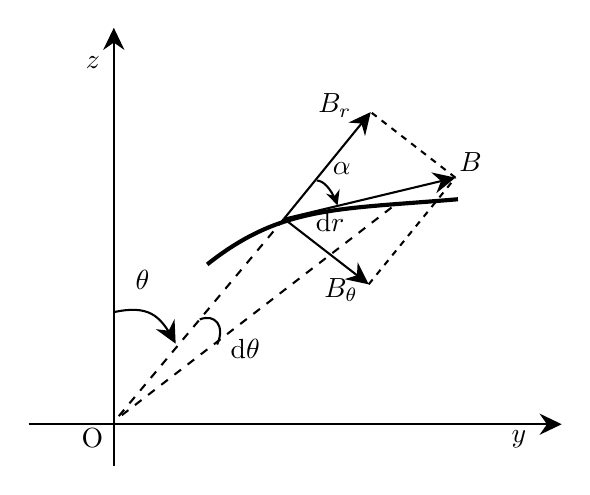
\begin{tikzpicture}[x=0.75pt,y=0.75pt,yscale=-1,xscale=1]
%uncomment if require: \path (0,520); %set diagram left start at 0, and has height of 520

%Straight Lines [id:da9063571252511462] 
\draw    (146,283) -- (399.8,283) ;
\draw [shift={(402.8,283)}, rotate = 180] [fill={rgb, 255:red, 0; green, 0; blue, 0 }  ][line width=0.08]  [draw opacity=0] (10.72,-5.15) -- (0,0) -- (10.72,5.15) -- (7.12,0) -- cycle    ;
%Straight Lines [id:da23780812775604465] 
\draw    (187,303) -- (187,95) ;
\draw [shift={(187,92)}, rotate = 450] [fill={rgb, 255:red, 0; green, 0; blue, 0 }  ][line width=0.08]  [draw opacity=0] (10.72,-5.15) -- (0,0) -- (10.72,5.15) -- (7.12,0) -- cycle    ;
%Straight Lines [id:da7758175564540406] 
\draw    (269,184) -- (308.91,134.93) ;
\draw [shift={(310.8,132.6)}, rotate = 489.12] [fill={rgb, 255:red, 0; green, 0; blue, 0 }  ][line width=0.08]  [draw opacity=0] (10.72,-5.15) -- (0,0) -- (10.72,5.15) -- (7.12,0) -- cycle    ;
%Straight Lines [id:da7825654978756766] 
\draw    (269,184) -- (307.43,213.76) ;
\draw [shift={(309.8,215.6)}, rotate = 217.76] [fill={rgb, 255:red, 0; green, 0; blue, 0 }  ][line width=0.08]  [draw opacity=0] (10.72,-5.15) -- (0,0) -- (10.72,5.15) -- (7.12,0) -- cycle    ;
%Straight Lines [id:da6487406086491123] 
\draw  [dash pattern={on 2.25pt off 2.25pt on 2.25pt off 2.25pt}]  (309.8,215.6) -- (351.6,164.2) ;
%Straight Lines [id:da8459463970687957] 
\draw  [dash pattern={on 2.25pt off 2.25pt on 2.25pt off 2.25pt}]  (351.6,164.2) -- (310.8,132.6) ;
%Straight Lines [id:da5599179201723574] 
\draw    (269,184) -- (348.68,164.9) ;
\draw [shift={(351.6,164.2)}, rotate = 526.52] [fill={rgb, 255:red, 0; green, 0; blue, 0 }  ][line width=0.08]  [draw opacity=0] (10.72,-5.15) -- (0,0) -- (10.72,5.15) -- (7.12,0) -- cycle    ;
%Curve Lines [id:da34507251510457126] 
\draw [line width=1.5]    (232,206) .. controls (267.8,177.6) and (294.8,179.6) .. (352.8,174.6) ;
%Straight Lines [id:da5497729013403247] 
\draw  [dash pattern={on 3pt off 3pt on 3pt off 3pt}]  (269,184) -- (187.8,281) ;
%Straight Lines [id:da1038316257756362] 
\draw  [dash pattern={on 3pt off 3pt on 3pt off 3pt}]  (320.8,178.6) -- (187.8,281) ;
%Curve Lines [id:da22526546545108328] 
\draw    (187,229) .. controls (203.55,225.47) and (209.04,230.41) .. (215.35,241.57) ;
\draw [shift={(216.8,244.2)}, rotate = 241.7] [fill={rgb, 255:red, 0; green, 0; blue, 0 }  ][line width=0.08]  [draw opacity=0] (10.72,-5.15) -- (0,0) -- (10.72,5.15) -- (7.12,0) -- cycle    ;
%Curve Lines [id:da16468632644450487] 
\draw    (228.4,232.5) .. controls (235.8,229.6) and (240.8,235.6) .. (236.8,244.6) ;
%Curve Lines [id:da7175480891950186] 
\draw    (284.8,165.6) .. controls (288.18,165.6) and (291.56,169.88) .. (293.73,174.83) ;
\draw [shift={(294.8,177.6)}, rotate = 251.57] [fill={rgb, 255:red, 0; green, 0; blue, 0 }  ][line width=0.08]  [draw opacity=0] (7.14,-3.43) -- (0,0) -- (7.14,3.43) -- (4.74,0) -- cycle    ;


% Text Node
\draw (172,104.4) node [anchor=north west][inner sep=0.75pt]    {$z$};
% Text Node
\draw (377.19,284.6) node [anchor=north west][inner sep=0.75pt]    {$y$};
% Text Node
\draw (196,207.4) node [anchor=north west][inner sep=0.75pt]    {$\theta $};
% Text Node
\draw (241.8,240.6) node [anchor=north west][inner sep=0.75pt]    {$\mathrm{d} \theta $};
% Text Node
\draw (282.8,179.6) node [anchor=north west][inner sep=0.75pt]    {$\mathrm{d} r$};
% Text Node
\draw (284,122.4) node [anchor=north west][inner sep=0.75pt]    {$B_{r}$};
% Text Node
\draw (287,211.4) node [anchor=north west][inner sep=0.75pt]    {$B_{\theta }$};
% Text Node
\draw (352,150.4) node [anchor=north west][inner sep=0.75pt]    {$B$};
% Text Node
\draw (291,155.4) node [anchor=north west][inner sep=0.75pt]    {$\alpha $};
% Text Node
\draw (170,283.4) node [anchor=north west][inner sep=0.75pt]    {$\mathrm{O}$};
\end{tikzpicture}
\end{center}

            Thay $\ot{M}.\ot{r}=Mr\cos \theta $ vào biểu thức rồi chiếu lên hai phương:
            \[\begin{aligned}
                {{B}_{r}} &= \dfrac{2{{\mu }_{0}}M}{4\pi }.\dfrac{\cos\theta }{{{r}^{3}}},\\
                {{B}_{\theta }} &= \dfrac{{{\mu }_{0}}M}{4\pi }.\dfrac{\sin \theta }{{{r}^{3}}}.
            \end{aligned}\]
            Phương trình đường sức từ là:
            \[r\dfrac{\dd \theta }{\dd r}=\dfrac{{{B}_{\theta }}}{{{B}_{r}}}=\dfrac{\sin\theta }{2\cos\theta},\]
            \[\Rightarrow r={{R}_{0}}{{\sin }^{2}}\theta,\] trong đó ${{R}_{0}}$ là bán kính ở mặt phẳng xích đạo.
            \\Từ đây tính được độ lớn từ trường dọc theo đường sức:
            \[B=\sqrt{B_{r}^{2}+B_{\theta }^{2}}=\dfrac{{{\mu }_{0}}M}{4\pi }\dfrac{\sqrt{1+3{{\cos }^{2}}\theta }}{{{r}^{3}}}=\dfrac{{{\mu }_{0}}M}{4\pi }\dfrac{\sqrt{1+3{{\cos }^{2}}\theta }}{R_{0}^{3}{{\sin }^{6}}\theta }={{B}_{0}}\dfrac{\sqrt{1+3{{\cos }^{2}}\theta }}{{{\sin }^{6}}\theta}.\]
        \end{enumerate}
        \item \begin{enumerate}[a)]
            \item Hạt chuyển động trong từ trường tĩnh thì động năng và vận tốc bảo toàn, chỉ thay đổi hướng chuyển động. Phương trình chuyển động có dạng:
            \[\dfrac{\dd\left( \ot{r}\times \ot{p} \right)}{\dd t}=e\ot{r}\times \left( \ot{v}\times \ot{B} \right)=e\left[ \ot{v}\left( \ot{r}.\ot{B} \right) - \ot{B}\left( \ot{v}.\ot{r} \right) \right],\]
            \[\Rightarrow \dfrac{d\left( \ot{r}\times {{{\ot{p}}}_{\theta }} \right)}{dt}+\dfrac{d\left( \ot{r}\times {{{\ot{p}}}_{\varphi }} \right)}{dt}=e\left[ r.{{B}_{r}}\ot{v}-r{{v}_{r}}\ot{B} \right].\]
            Thành phần thứ nhất ở vế trái vuông góc với mặt phẳng kinh độ nên khi chiếu lên sẽ bằng không. Thành phần thứ hai có độ lớn $r{{p}_{\varphi }}$, có phương nằm trong mặt phẳng kinh độ và vuông góc với $\ot{r}$, do đó nó làm với Oz một góc $\dfrac{\pi }{2}-\theta$. \\Vậy hình chiếu của moment động lượng lên trục Oz là $r\sin \theta .{{p}_{\varphi }}$.
            \\Vậy:\[\begin{aligned}
                \dfrac{\dd\left( r\sin \theta .{{p}_{\varphi }} \right)}{\dd t}&=er\left[ {{B}_{r}}\left( {{v}_{r}}\cos \theta -{{v}_{\theta }}\sin \theta  \right)-{{v}_{r}}\left( {{B}_{r}}\cos \theta -{{B}_{\theta }}\sin \theta  \right) \right]\\
                &=er\sin \theta \left( {{v}_{r}}{{B}_{\theta }}-{{v}_{\theta }}{{B}_{r}} \right).
            \end{aligned}\]
            Thay biểu thức của cảm ứng từ và vận tốc vào vế phải được
            \[\begin{aligned}
                \dfrac{\dd\left( r\sin \theta .{{p}_{\varphi }} \right)}{\dd t}&=er\sin \theta \left( \dfrac{\dd r}{\dd t}\dfrac{{{\mu }_{0}}M}{4\pi }\dfrac{\sin \theta}{{{r}^{3}}}-r\dfrac{\dd\theta }{\dd t}.\dfrac{{{\mu }_{0}}M}{4\pi }\dfrac{2\cos \theta }{{{r}^{3}}} \right)\\
                &=-\dfrac{\dd}{\dd t}\left( \dfrac{e{{\sin }^{2}}\theta }{r}\dfrac{{{\mu }_{0}}M}{4\pi } \right).
            \end{aligned}\]
            \[\Rightarrow r\sin \theta .{{p}_{\varphi }}+\dfrac{e{{\sin }^{2}}\theta }{r}\dfrac{{{\mu }_{0}}M}{4\pi } = \const.\]
            Thay ${{p}_{\varphi}}=mr\sin \theta \dfrac{\dd\varphi}{\dd t}$ vào ta được: 
            \[\const = m {{r}^{2}}{{\sin }^{2}}\theta \dfrac{\dd\varphi }{\dd t}+\dfrac{e{{\sin }^{2}}\theta }{r}.\dfrac{{{\mu }_{0}}M}{4\pi }={{\sin }^{2}}\theta \left( m{{r}^{2}}\dfrac{\dd\varphi }{\dd t}+\dfrac{{{\mu }_{0}}}{4\pi }\dfrac{eM}{r} \right).\]
            \item Các đường sức từ vuông góc với mặt phẳng xích đạo nên nếu ban đầu vận tốc hạt thuộc mặt phẳng xích đạo thì lực Lorentz cũng sẽ thuộc mặt phẳng xích đạo. Kết quả là hạt chỉ chuyển động trong mặt phẳng xích đạo có $\theta =\dfrac{\pi }{2}$.
            \\Bất biến câu $a)$ có dạng \[r{{p}_{\varphi }}+\dfrac{{{\mu }_{0}}Me}{4\pi r}={{L}_{z}}+\dfrac{{{\mu }_{0}}Me}{4\pi r}=\const=A.\]
            Hằng số được xác định từ điều kiện ban đầu khi $r=\infty ,A={{L}_{z\infty }}=\pm bp$, dấu $\pm $ tuỳ thuộc vào hạt lao đến chếch Đông hay Tây.
            \\Biến đổi ${{p}_{\varphi }}=\dfrac{A}{r}-\dfrac{{{\mu }_{0}}Me}{4\pi {{r}^{2}}}$.
            \\Điểm tiếp cận cực tiểu của hạt được xác định bởi $p_{r}^{2}={{p}^{2}}-p_{\varphi }^{2}=0$ hay $p=\left| {{p}_{\varphi }} \right|$.
            \\Nếu lấy dấu ``$-$'' ta biến đổi được phương trình: \[{{r}^{2}}-br-\dfrac{{{\mu }_{0}}Me}{4\pi p}=0.\]
            Phương trình này có nghiệm:
            \[r=\dfrac{1}{2}\left( b+\sqrt{{{b}^{2}}+\dfrac{{{\mu }_{0}}Me}{\pi p}} \right).\]
            Tương tự với dấu ``$+$'', ta tính được: \[r=\dfrac{1}{2}\left( b+\sqrt{{{b}^{2}}-\dfrac{{{\mu }_{0}}Me}{\pi p}} \right).\]
        \end{enumerate}
        \item\begin{enumerate}[a)]
            \item Bán kính quay được xác định từ điều kiện cân bằng lực ly tâm và lực Lorentz:
             \[\dfrac{mv_{\perp }^{2}}{\rho }=e{{v}_{\perp }}B
             \Rightarrow \rho =\dfrac{m{{v}_{\perp }}}{eB}=\dfrac{{{p}_{\perp}}}{eB}
             \Rightarrow {{\omega}_{c}}=\dfrac{eB}{m}.\]
            \item Từ thông gửi qua vòng dây $\Phi =\pi {{\rho }^{2}}B$.
            \\Áp dụng định luật II Newton: \[\dfrac{\dd{{p}_{\perp }}}{\dd t}=e{{E}_{c}}=\dfrac{e\rho }{2}.\dfrac{\dd B}{\dd t}=\dfrac{{{p}_{\perp  }}}{2B}\dfrac{\dd B}{\dd t}.\]
            Rút gọn $\dd t$ rồi tích phân, ta thu được: 
            \[\dfrac{p_{\perp }^{2}}{B}=\const.\]
            Dòng điện cho hạt tạo ra 
            \[I=e\dfrac{{{\omega }_{c}}}{2\pi }.\]
            Moment từ 
            \[\mu =\pi {{\rho }^{2}}I=\dfrac{{{\rho }^{2}}eqB}{2m}=\const.\]
            \item Từ điều kiện:
            \[\dfrac{p_{\perp}^{2}}{B}=\dfrac{{{p}^{2}}{{\sin }^{2}}\alpha }{B}=\const = \dfrac{{{p}^{2}}{{\sin }^{2}}{{\alpha }_{0}}}{{{B}_{0}}}.\]
            Tại điểm gương $\sin {{\alpha }_{m}}=1$, suy ra: ${{\sin }^{2}}{{\alpha }_{0}}=\dfrac{{{B}_{0}}}{{{B}_{m}}}$.
            \\Thay biểu thức của $B$ từ phần $1c)$ vào ta được: 
        	\[{{\sin }^{2}}{{\alpha }_{0}}=\dfrac{{{\sin }^{6}}{{\theta }_{m}}}{\sqrt{1+3{{\cos }^{2}}{{\theta }_{m}}}}.\]
            \item Gọi $s$ là tọa độ tự nhiên dọc theo đường sức $t$. Ta có ${{v}_{\parallel}}=\dfrac{\dd s}{\dd t}$, suy ra:
            \[{{\tau }_{2}}=4\int\limits_{\pi /2}^{{{\theta }_{m}}}{\dfrac{\dd s}{{{v}_{\parallel}}}}=\dfrac{4}{v}\int\limits_{\pi /2}^{{{\theta }_{m}}}{\dfrac{\dd s}{\cos \alpha }}.\]
            Mặt khác,
            \[\cos \alpha =\sqrt{1-{{\sin }^{2}}\alpha }=\sqrt{1-\dfrac{B}{{{B}_{0}}}{{\sin }^{2}}{{\alpha }_{0}}}=\sqrt{1-\dfrac{\sqrt{1+3{{\cos }^{2}}\theta }}{{{\sin }^{6}}\theta }{{\sin }^{2}}{{\alpha }_{0}}}.\]
            Lại có:
            \[\begin{aligned}
                \dd s&=\sqrt{{{\left( \dd r \right)}^{2}}+{{\left( r\dd \theta  \right)}^{2}}}\\
                &=\sqrt{{{\left( 2{{R}_{0}}\sin \theta \cos \theta \dd \theta  \right)}^{2}}+{{\left( {{R}_{0}}{{\sin }^{2}}\theta \dd\theta  \right)}^{2}}}\\
                &={{R}_{0}}\sin \theta \sqrt{1+3{{\cos }^{2}}\theta }.\dd\theta.
            \end{aligned}
             \]
            Vậy: 
            \[{{\tau }_{2}}=\dfrac{4{{R}_{0}}}{v}\int\limits_{\pi /2}^{{{\theta }_{m}}}{\dfrac{{{\sin }^{4}}\theta \sqrt{1+3{{\cos }^{2}}\theta }}{\sqrt{{{\sin }^{6}}\theta -{{\sin }^{2}}{{\alpha }_{0}}\sqrt{1+3{{\cos }^{2}}\theta }}}\dd\theta }=\dfrac{4{{R}_{0}}}{v}f\left( \sin {{\alpha }_{0}} \right).\]
            \item Từ câu $2c)$, xác định: 
            \[\dfrac{\dd\varphi }{\dd t}=\dfrac{1}{m{{r}^{2}}}\left( \dfrac{A}{{{\sin }^{2}}\theta }-\dfrac{{{\mu }_{0}}eM}{4\pi r} \right)=\left( \dfrac{A}{R_{0}^{2}}-\dfrac{{{\mu }_{0}}eM}{4\pi R_{0}^{3}} \right)\dfrac{1}{m.{{\sin }^{6}}\theta }.\]
            Tính góc mà mặt kinh tuyến quay được sau một chu kì chuyển động trượt của tâm quay từ điểm gương cực Bắc đến điểm gương cực Nam rồi quay trở lại.
            \[\begin{aligned}
              \Delta \varphi &= 4\int\limits_{\pi /2}^{{\theta _m}} {\dfrac{{\dd\varphi }}{{\dd t}}}  = 4\int\limits_{\pi /2}^{{\theta _m}} {\dfrac{{\dd\varphi }}{{\dd t}}\dfrac{{\dd{{s}}}}{{{v_{\parallel}}}}}\\
              &=\dfrac{4}{{mv}}\left( {\dfrac{A}{{{R_0}}} - \dfrac{{{\mu _0}eM}}{{4\pi R_0^2}}} \right)\int\limits_{\pi /2}^{{\theta _m}} {\dfrac{{\sqrt {1 + 3{{\cos }^2}\theta } }}{{{{\sin }^2}\theta \sqrt {{{\sin }^6}\theta  - {{\sin }^2}{\alpha _0}\sqrt {1 + 3{{\cos }^2}\theta } } }}\dd\theta } \\
              &=\dfrac{4}{{mv}}\left( {\dfrac{A}{{{R_0}}} - \dfrac{{{\mu _0}eM}}{{4\pi R_0^2}}} \right)g\left( {\sin {\alpha _0}} \right).
            \end{aligned}\]
                Do vậy 
                \[{{\tau }_{3}}=\dfrac{2\pi }{\Delta \varphi }.\]

        \end{enumerate}
    \end{enumerate}
\end{loigiai}


\begin{vd}[Đơn cực và Dyon]
%IOM 2019
Ngay từ thế kỉ $18$, thông qua thực nghiệm Chales Coulomb đã thiết lập các quy luật tương tác của các điện tích và các cực của nam châm là giống hệt nhau. Sau đó, nhiều nghiên cứu đã cố gắng tách hai cực của nam châm để thu được một điện tích từ ``duy nhất'' và đặt tên là ``đơn cực từ''. Tuy nhiên, tất cả các nam châm đã biết từ kích thước vĩ mô tới kích thước hạt cơ bản đều trở thành một lưỡng cực từ, tức là nó luôn luôn có cả hai cực từ. Vào thế kỉ $19$, André-Marie Ampère đã chỉ ra rằng trường của lưỡng cực từ có thể tạo ra được bởi một vòng dây dẫn điện nhỏ, do đó, không cần phải giả thiết sự tồn tại của đơn cực từ để mô tả các hiện tượng quan sát được.\\
Vào thế kỉ $20$, Paul Dirac đã đề xuất một ý tưởng về cách tạo ra một đơn cực từ ``nhân tạo'': một ống solenoid mềm, rất mỏng và rất dài (có chiều dài $l$ và mặt cắt có tiết diện $S$, với $l\gg \sqrt{S}$), ống gồm $N$ vòng dây và mang một dòng điện $I$. Từ thông trong lòng ống solenoid đi ra khỏi đầu ống theo mọi hướng và có phương xuyên tâm. Do đó, từ trường ở gần đầu ống solenoid (ở mọi nơi ngoại trừ trên chính ống solenoid) giống với từ trường tạo ra bởi một đơn cực từ có điện tích từ $M=\dfrac{NIS}{l}$. Cảm ứng từ của đơn cực từ là $\ot{B}\approx \dfrac{\mu_0M}{4\pi r^3}\ot{r}$, trong đó $\mu_0\approx4\pi\cdot 10^{-7} ~\mathrm{H/m}$ là hằng số từ (độ từ thẩm chân không). Sau đó ý tưởng này đã được tiến hành thực nghiệm: với một xoáy trong chất lỏng hoặc chất khí lượng tử đóng vai trò như một ống solenoid. Hai ``đầu'' của ống solenoid ở xa và di chuyển gần như độc lập, từ đó tạo ra ``ảnh'' của hai đơn cực nằm trong hệ thống. Các đường sức từ đi từ các đầu của ống solenoid một cách hướng tâm và lan ra đối xứng cầu như đường sức điện tạo ra bởi điện trường của một điện tích điểm.\\
Năm $1974$, Alexander Polyakov và Gerard t'Hooft đã phát hiện ra các đơn cực từ ``thật'' với một điện tích từ khác không phải tồn tại trong lí thuyết thực tế về các hạt cơ bản. Do đó, việc tích cực thực hiện các thí nghiệm về các hạt như vậy vẫn tiếp tục diễn ra tới cả thế kỉ $21$.\\
\begin{center}
    \textbf{Phần I: Phát hiện dấu vết của đơn cực từ}
\end{center}
Một trong những phương pháp phát hiện đơn cực từ là đo dòng điện khi đơn cực từ đi qua một vòng dây dẫn. Các thiết bị dò đơn cực từ hiện nay thường sử dụng các vòng dây siêu dẫn (hay còn gọi là SQUID $-$ Thiết bị giao thoa lượng tử siêu dẫn).
\begin{enumerate}[1)]
    \item Một đơn cực từ chuyển động với tốc độ lớn dọc theo trục của một vòng siêu dẫn mỏng và đi xuyên qua vòng. Hãy vẽ đồ thị biểu diễn sự phụ thuộc của dòng điện cảm ứng $I$ theo thời gian. Lấy chiều dương của dòng điện là khi đơn cực từ tiến gần tới vòng. Giả sử rằng tại $t=0$, đơn cực nằm trong mặt phẳng của vòng. Đồ thị của bạn cần phải biểu diễn được các điểm quan trọng.\\
    Cho điện tích từ của đơn cực là $M=\tron{4\cdot10^{-8}~\mathrm{C\cdot H\cdot s^{-1}}}/\mu_0$ và khối lượng của nó là $m=1 ~\mu \mathrm{g}$, bán kính của vòng là $a=1~\mathrm{m}$, và giả sử rằng vòng được làm bằng dây có bán kính $r=0.5~\mathrm{mm}$. Độ tự cảm của vòng dây được cho gần đúng bởi công thức Grover: \[L\approx\mu_0a\left[\ln\tron{\dfrac{8a}{r}}-\dfrac{7}{4}\right].\]
    \item Giả sử rằng, vận tốc của đơn cực khi ở một khoảng cách khá lớn so với vòng ($x_0\gg a$) là $v_0=1~\mathrm{km/s}.$ Gọi $x$ là khoảng cách hiện tại giữa vòng và đơn cực. Cả hệ được đặt trong chân không và đơn cực di chuyển dọc theo trục của vòng. Hãy xác định cường độ dòng điện cảm ứng $I\tron{x}$ lúc này. Giá trị cực đại $I_{\max}^S$ của dòng điện cảm ứng là bao nhiêu? Bỏ qua bức xạ điện từ của hệ, hãy xác định độ biến thiên cực đại của vận tốc đơn cực $\tron{v_0-v_{\min}}$ trong quá trình chuyển động. \\
    Đáp án của bạn phải bao gồm một phương trình của $I$, một phương trình và giá trị bằng số của $I_{\max}^S$ theo đơn vị $\mathrm{mA}$, và một phương trình và giá trị bằng số cho độ biến thiên vận tốc theo đơn vị $\mathrm{m/s}$.\\
    \textbf{Gợi ý toán học.} Góc khối giới hạn bởi hình nón có góc ở đỉnh là $2\alpha$ có giá trị là \[\Omega=2\pi\cdot \left[1-\cos\alpha\right].\]
    Sau đó, bạn nên nghiên cứu rằng điện trở suất của vòng sẽ ảnh hưởng như thế nào đến hình dạng xung của dòng điện cảm ứng và chuyển động của đơn cực.
    \item Giả sử rằng, đơn cực từ chuyển động với vận tốc lớn dọc theo trục của một vòng nhẫn mảnh dẫn điện và đi qua vòng nhẫn.
    \begin{enumerate}[a)]
        \item Vẽ biểu đồ sự phụ thuộc của dòng điện cảm ứng $I$ chạy qua vòng nhẫn theo thời gian $t$. Điện trở của vòng nhẫn có độ lớn là: $R\gg\dfrac{Lv_0}{2r}.$
        \item Vẽ biểu đồ biểu diễn sự phụ thuộc $I\tron{t}$ với cùng chuyển động của đơn cực khi vòng nhẫn có điện trở ``trung bình'': $\dfrac{Lv_0}{a}\ll R\ll\dfrac{Lv_0}{2r}.$
        \item Để so sánh, hãy vẽ sự phụ thuộc của $I\tron{t}$ với trường hợp một nam châm hình trụ mỏng đi qua vòng nhẫn có điện trở lớn (trục của nam châm trùng với trục của vòng nhẫn).\\
        Trong mọi trường hợp, chiều dương của dòng điện cảm ứng tương ứng với lúc vật chuyển động lại gần vòng nhẫn. Giả sử rằng đơn cực (hoặc tâm của nam châm hình trụ) nằm trong mặt phẳng của vòng nhẫn lúc $t=0$. Vẽ đồ thị định tính thể hiện tất cả các đặc điểm quan trọng của sự phụ thuộc được vẽ.\\
        Hãy xem xét một tình huống được miêu tả trong phần $2)$, nhưng với vòng nhẫn có điện trở suất $\rho=10^{-8}~\mathrm{\Omega\cdot m}$ (và cùng các giá trị số của $a,r,M,m$ và $v_0$).
        \end{enumerate}
        \item Tại một thời điểm nào đó, đơn cực ở khoảng cách $x\gg r$ so với tâm của vòng nhẫn và di chuyển với tốc độ $v\tron{x}$. Giá trị của dòng điện cảm ứng $I\tron{x}$ ở thời điểm này là bao nhiêu? Bỏ qua bức xạ điện từ, hãy ước tính sự thay đổi vận tốc của đơn cực sau khi đi qua vòng nhẫn (tức là khi đơn cực đã ở xa vòng). Đáp án của bạn phải bao gồm phương trình của $I$ và giá trị số của sự thay đổi vận tốc theo $\mathrm{m/s}$.
    \end{enumerate}
\begin{center}
    \textbf{Phần II: Dyon và quỹ đạo tròn}
    \end{center}
    Ngoài các đơn cực, nhiều lí thuyết của vật lí năng lượng cao còn dự đoán có các hạt giả định mang cả điện tích và từ tích (hay còn gọi là các hạt dyon).\\
    Giả sử rằng, có một hạt nhẹ khối lượng $m$ mang điện tích $q$ di chuyển trong trường của một hạt dyon rất nặng với điện tích $Q>0$ và điện tích từ $M>0$. Lưu ý rằng, hằng số điện (độ điện thẩm chân không) $\varepsilon_0$ trong định luật Coulomb liên hệ với hằng số từ (độ từ thẩm chân không) theo công thức: $\dfrac{1}{\varepsilon_0\mu_0}=c^2$, trong đó $c\approx3\cdot10^8~\mathrm{m/s}$ là tốc độ ánh sáng trong chân không.
    \begin{enumerate}[1)]
        \item Hạt được kích thích chuyển động trong trường của dyon với quỹ đạo tròn và vận tốc không đổi $v\ll c$ (bức xạ điện từ ở vận tốc này là không đáng kể). Hãy xác định một bán kính có thể của quỹ đạo. Câu trả lời phải được biểu diễn dưới dạng một hàm số. Hãy phác họa dyon, hạt và quỹ đạo của nó.
        \item Chỉ ra vị trí quỹ đạo của hạt so với dyon (xác định tất cả thông số hình học cần thiết và viết ra các công thức tương ứng). Xác định các thông số này trên đồ thị phác thảo ở phần $1)$.
        \item Xác định đại lượng tích phân của chuyển động (một vô hướng và một vector) không đổi trong suốt quá trình chuyển động của hạt mang điện trong trường của dyon. Biểu diễn các tích phân này qua tọa độ của hạt $\ot{r}$ và vận tốc $\ot{v}$ (các công thức này cũng phải bao gồm các tham số của hệ). Tìm công thức tính tích phân cho quỹ đạo của chuyển động tròn đã nói ở trên (kết quả phải được biểu diễn dưới dạng phương trình bao gồm các tham số của hệ và $v$).\\
        \textbf{Gợi ý.} Tích phân vector tại $M=0$ phải trở thành moment động lượng của hạt, và rõ ràng moment động lượng được bảo toàn trong suốt quá trình chuyển động của hạt trong trường của một điện tích điểm. Khi $M\ne 0$, vector tích phân bằng với moment động lượng thực của hệ bao gồm dyon, hạt và trường điện từ của chúng.\\
        \textbf{Gợi ý toán học.} Phương trình sau có thể hữu ích:
        $$\dfrac{\dd}{\dd t}\tron{\dfrac{1}{r}}=-\dfrac{\tron{\dfrac{\dd r}{\dd t}}}{r^2}=-\dfrac{\tron{\ot{v}\ot{r}}}{r^3}.$$
    \end{enumerate}
\begin{center}
    \textbf{Phần III: Đơn cực từ và lượng tử hóa điện tích}
    \end{center}
Xét một hạt có khối lượng $m$ và điện tích $q$ di chuyển trong trường của một đơn cực đứng yên với điện tích từ $M$. Hạt bắt đầu chuyển động ở rất xa đơn cực với vận tốc $v_0$, với tham số va chạm là $b$ (khoảng cách vuông góc giữa đơn cực và đường ngoại suy của hạt). Giá trị của $b$ được chọn sao cho khi hạt đi qua đơn cực và đi ra xa khỏi nó, hạt sẽ chuyển động trên một mặt phẳng song song với mặt phẳng của hình vẽ ở khoảng cách $d$.
\begin{center}
\tikzset{every picture/.style={line width=0.75pt}} %set default line width to 0.75pt        

\begin{tikzpicture}[x=0.75pt,y=0.75pt,yscale=-1,xscale=1]
%uncomment if require: \path (0,385); %set diagram left start at 0, and has height of 385

%Straight Lines [id:da026936104845926234] 
\draw  [dash pattern={on 4.5pt off 4.5pt}]  (130.5,130.5) -- (355.5,130.5) ;
%Straight Lines [id:da45120183734844255] 
\draw  [dash pattern={on 4.5pt off 4.5pt}]  (130.5,40) -- (355.5,40) ;
%Straight Lines [id:da3076635941597241] 
\draw    (200.5,43.5) -- (200.5,128) ;
\draw [shift={(200.5,131)}, rotate = 270] [fill={rgb, 255:red, 0; green, 0; blue, 0 }  ][line width=0.08]  [draw opacity=0] (8.04,-3.86) -- (0,0) -- (8.04,3.86) -- (5.34,0) -- cycle    ;
\draw [shift={(200.5,40.5)}, rotate = 90] [fill={rgb, 255:red, 0; green, 0; blue, 0 }  ][line width=0.08]  [draw opacity=0] (8.04,-3.86) -- (0,0) -- (8.04,3.86) -- (5.34,0) -- cycle    ;
%Straight Lines [id:da7905109218103124] 
\draw    (299,40) -- (255.5,40) ;
\draw [shift={(252.5,40)}, rotate = 360] [fill={rgb, 255:red, 0; green, 0; blue, 0 }  ][line width=0.08]  [draw opacity=0] (7.14,-3.43) -- (0,0) -- (7.14,3.43) -- (4.74,0) -- cycle    ;
\draw [shift={(299,40)}, rotate = 180] [color={rgb, 255:red, 0; green, 0; blue, 0 }  ][fill={rgb, 255:red, 0; green, 0; blue, 0 }  ][line width=0.75]      (0, 0) circle [x radius= 2.01, y radius= 2.01]   ;
%Shape: Circle [id:dp02579023264128133] 
\draw  [fill={rgb, 255:red, 0; green, 0; blue, 0 }  ,fill opacity=1 ] (153,129.75) .. controls (153,127.96) and (154.46,126.5) .. (156.25,126.5) .. controls (158.04,126.5) and (159.5,127.96) .. (159.5,129.75) .. controls (159.5,131.54) and (158.04,133) .. (156.25,133) .. controls (154.46,133) and (153,131.54) .. (153,129.75) -- cycle ;

% Text Node
\draw (149,105.9) node [anchor=north west][inner sep=0.75pt]    {$M$};
% Text Node
\draw (207,76.4) node [anchor=north west][inner sep=0.75pt]    {$b$};
% Text Node
\draw (294,47.4) node [anchor=north west][inner sep=0.75pt]    {$q$};
% Text Node
\draw (247.5,11.4) node [anchor=north west][inner sep=0.75pt]    {$\overrightarrow{v_{0}}$};


\end{tikzpicture}

\end{center}
\begin{enumerate}[1)]
    \item Hãy xác định vận tốc $v'$ của hạt sau khi nó ra khỏi trường của đơn cực (tức là khi hạt ở rất xa so với đơn cực). Câu trả lời phải được đưa ra dưới dạng công thức bao gồm các đại lượng được nêu ở trên.
    \item Xác định tất cả các giá trị có thể của góc tán xạ (góc giữa $\ot{v'}$ và $\ot{v_0}$). Câu trả lời phải được đưa ra dưới dạng công thức bao gồm các đại lượng được nêu trên.
    \item Xác định khoảng cách vuông góc $b'$ giữa đơn cực và đường đi của hạt sau tán xạ. Câu trả lời phải được đưa ra dưới dạng công thức bao gồm các đại lượng được nêu trên.\\
    Trong vật lí cổ điển, các điện tích và từ tích có thể nhận các giá trị tùy ý, tuy nhiên, trong lí thuyết lượng tử, điều này không còn đúng nữa. Vấn đề là trong thuyết lượng tử, moment động lượng của một hạt (hay còn gọi là moment quỹ đạo) và moment động lượng của trường điện từ phải tuân theo quy luật lượng tử hóa của moment động lượng: bất kì thành phần vector nào của moment động lượng phải là bội của hằng số $\dfrac{\hbar}{2}\equiv\dfrac{h}{4\pi}$, trong đó $h\approx 6,63\cdot10^{-34}~\mathrm{J\cdot s}$ là hằng số Planck.
    \item Hãy xét một hạt mang điện tích $q$ chuyển động trong trường của điện tích từ $M$ và sử dụng định luật lượng tử moment động lượng. Xác định điều kiện liên hệ giữa $q$ và $M$, sao cho các định luật bảo toàn đặc trưng của bài toán này và định luật lượng tử moment động lượng không mâu thuẫn với nhau. Xác định giá trị của từ tích mà điện tích bất kì là bội số của điện tích cơ bản $e\approx 1,6\cdot 10^{-19}~\mathrm{C}$. Câu trả lời phải đưa ra dưới dạng một công thức liên hệ giữa từ tích và điện tích và giá trị số của $M$ có đơn vị $\mathrm{C\cdot m/s}$. 
\end{enumerate}
\end{vd}
\begin{loigiai}
  \begin{center}
     \textbf{Phần I}
   \end{center}
 \begin{enumerate}[1)]
   \item Chúng ta có hai cách giải cho phần này.\\
\textbf{Cách 1.} Chúng ta có thể áp dụng các phương trình điện động lực học cho từ tích để tính đối xứng của các phương trình điện động lực học được bảo toàn khi chúng ta thay từ tích thành điện tích và do đó từ trường thành điện trường (như có thể thấy trong đề bài, từ trường gây ra bởi một từ tích tĩnh hoàn toàn trùng khít với điện trường gây ra bởi một điện tích tĩnh nếu chúng ta thay thế một số đại lượng tương đương $M \leftrightarrow q, \mu_0 \leftrightarrow \dfrac{1}{\varepsilon_0}, \ot{B} \leftrightarrow \ot{E}$). Như ta đã biết, điện tích chuyển động gây ra từ trường. Điện trường của một điện tích điểm tĩnh là: 
    \[\ot{E} = \dfrac{q}{4\pi \varepsilon_0 r^3} \ot{r},\]

ở đây $\ot{r}$ là khoảng cách từ điện tích đến vị trí quan sát $P$, do đó $\ot{r} \equiv \ot{r_P} -\ot{\rho}(t)$ (ở đây $\ot{\rho}(t)$ là khoảng cách từ điện tích điểm đến gốc tọa độ của hệ quy chiếu). Từ trường gây ra bởi một điện tích điểm chuyển động có thể được tính ra từ định luật Biot $-$ Savart $-$ Laplace:
  \[ \ot{B} = \dfrac{\mu_0 q}{4\pi r^3} \left[\ot{v} \times \ot{r}\right].\]
Do đó, với điện tích điểm chuyển động với vận tốc $\ot{v}$, từ trường
    \[\ot{B} = \dfrac{1}{c^2} \left[\ot{v} \times \ot{E}\right].\]

Ghi nhớ rằng, từ suy luận của chúng ta về tính đối xứng, ta có thể kết luận rằng từ tích khi chuyển động sẽ gây ra điện trường
  \[\ot{E} = \left[\ot{v} \times \ot{B}\right].\]

\textbf{Lưu ý.} Đây là điện trường gây ra bởi từ tích chuyển động với vận tốc không đổi (vì nếu có gia tốc, điện tích sẽ phát xạ sóng điện từ).
\begin{center}


\tikzset{every picture/.style={line width=0.75pt}} %set default line width to 0.75pt        

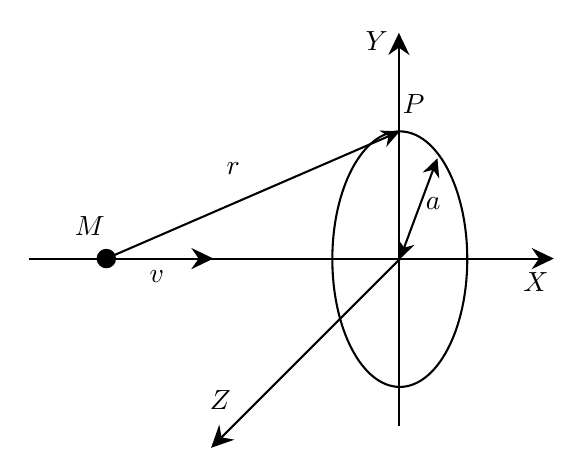
\begin{tikzpicture}[x=0.75pt,y=0.75pt,yscale=-1,xscale=1]
%uncomment if require: \path (0,300); %set diagram left start at 0, and has height of 300

%Straight Lines [id:da9053986049845555] 
\draw    (173.2,158.14) -- (423.2,158.14) ;
\draw [shift={(426.2,158.14)}, rotate = 180] [fill={rgb, 255:red, 0; green, 0; blue, 0 }  ][line width=0.08]  [draw opacity=0] (10.72,-5.15) -- (0,0) -- (10.72,5.15) -- (7.12,0) -- cycle    ;
%Straight Lines [id:da7197795073726467] 
\draw    (351.55,238.68) -- (351.55,52.4) ;
\draw [shift={(351.55,49.4)}, rotate = 450] [fill={rgb, 255:red, 0; green, 0; blue, 0 }  ][line width=0.08]  [draw opacity=0] (10.72,-5.15) -- (0,0) -- (10.72,5.15) -- (7.12,0) -- cycle    ;
%Shape: Ellipse [id:dp029446166013577413] 
\draw   (319.48,158.42) .. controls (319.48,124.43) and (334.03,96.86) .. (351.98,96.86) .. controls (369.94,96.86) and (384.49,124.43) .. (384.49,158.42) .. controls (384.49,192.42) and (369.94,219.98) .. (351.98,219.98) .. controls (334.03,219.98) and (319.48,192.42) .. (319.48,158.42) -- cycle ;
%Shape: Circle [id:dp09591599147663277] 
\draw  [fill={rgb, 255:red, 0; green, 0; blue, 0 }  ,fill opacity=1 ] (206.43,158.14) .. controls (206.43,155.83) and (208.29,153.97) .. (210.6,153.97) .. controls (212.9,153.97) and (214.77,155.83) .. (214.77,158.14) .. controls (214.77,160.44) and (212.9,162.31) .. (210.6,162.31) .. controls (208.29,162.31) and (206.43,160.44) .. (206.43,158.14) -- cycle ;
%Straight Lines [id:da10566926190415726] 
\draw    (210.6,158.14) -- (349.23,98.06) ;
\draw [shift={(351.98,96.86)}, rotate = 516.5699999999999] [fill={rgb, 255:red, 0; green, 0; blue, 0 }  ][line width=0.08]  [draw opacity=0] (8.93,-4.29) -- (0,0) -- (8.93,4.29) -- (5.93,0) -- cycle    ;
%Straight Lines [id:da0780199842880096] 
\draw    (353.03,155.61) -- (369.06,112.62) ;
\draw [shift={(370.11,109.81)}, rotate = 470.44] [fill={rgb, 255:red, 0; green, 0; blue, 0 }  ][line width=0.08]  [draw opacity=0] (8.93,-4.29) -- (0,0) -- (8.93,4.29) -- (5.93,0) -- cycle    ;
\draw [shift={(351.98,158.42)}, rotate = 290.44] [fill={rgb, 255:red, 0; green, 0; blue, 0 }  ][line width=0.08]  [draw opacity=0] (8.93,-4.29) -- (0,0) -- (8.93,4.29) -- (5.93,0) -- cycle    ;
%Straight Lines [id:da4094706029412589] 
\draw    (351.98,158.42) -- (263.2,247.2) ;
\draw [shift={(261.08,249.33)}, rotate = 315] [fill={rgb, 255:red, 0; green, 0; blue, 0 }  ][line width=0.08]  [draw opacity=0] (10.72,-5.15) -- (0,0) -- (10.72,5.15) -- (7.12,0) -- cycle    ;
%Straight Lines [id:da16293219599151443] 
\draw    (210.6,158.14) -- (259.2,158.14) ;
\draw [shift={(262.2,158.14)}, rotate = 180] [fill={rgb, 255:red, 0; green, 0; blue, 0 }  ][line width=0.08]  [draw opacity=0] (10.72,-5.15) -- (0,0) -- (10.72,5.15) -- (7.12,0) -- cycle    ;


% Text Node
\draw (267,110.4) node [anchor=north west][inner sep=0.75pt]    {$\ot{r}$};
% Text Node
\draw (230,162.4) node [anchor=north west][inner sep=0.75pt]    {$\ot{v}$};
% Text Node
\draw (194,136.4) node [anchor=north west][inner sep=0.75pt]    {$M$};
% Text Node
\draw (363,127.4) node [anchor=north west][inner sep=0.75pt]    {$a$};
% Text Node
\draw (334,47.4) node [anchor=north west][inner sep=0.75pt]    {$Y$};
% Text Node
\draw (410,163.4) node [anchor=north west][inner sep=0.75pt]    {$X$};
% Text Node
\draw (259,220.4) node [anchor=north west][inner sep=0.75pt]    {$Z$};
% Text Node
\draw (352,77.4) node [anchor=north west][inner sep=0.75pt]    {$P$};


\end{tikzpicture}
\end{center}
Tiếp theo, chúng ta xem xét trường hợp một từ tích chuyển động xuyên qua một vòng dây siêu dẫn. Chúng ta sử dụng một hệ tọa độ như trên hình vẽ: gốc tọa độ là tâm của vòng dây, trục $X$ dọc theo trục đối xứng của vòng dây, trục $Y$ hướng từ tâm tới một điểm $P$ trên vòng dây. Vận tốc của đơn cực, $\ot{v} = v\cdot \ot{e_x} $, phương trình chuyển động của nó $\ot{\rho}(t) = vt\cdot \ot{e_x}$, và $\ot{r_p} = a\ot{e_y}$. Điện trường mà đơn cực từ tạo ra ở vị trí của điểm $P$ là:
      \[\ot{E} = \left[\ot{v} \times \ot{B}\right] = \dfrac{\mu_0 M}{4\pi r^3}\left[(v\ot{e_x})\times (a\ot{e_y} - vt\ot{e_x}) \right] = \dfrac{\mu_0  M}{4\pi} \cdot \dfrac{av}{(a^2 + v^2t^2)^{3/2}}\ot{e_z}.\]

Vì điện trường này là đối xứng xung quanh trục $x$, điện trường trong vòng tạo ra một suất điện động cảm ứng có độ lớn
  \[U_E = E\cdot 2\pi a = \dfrac{\mu_0 M}{2} \cdot \dfrac{a^2}{(a^2 + v^2t^2 )^{3/2}}v.\]

Suất điện động cảm ứng ở trên vòng dây siêu dẫn luôn phải bằng không với mọi giá trị dòng điện. Suất điện động này gồm hai thành phần, thành phần ngoài do điện trường của từ tích gây ra và thành phần nội tại do hiện tượng tự cảm $U_L = -L \dfrac{\dd I}{\dd t}$. Suất điện động cảm ứng thu được ở trên có thể được viết dưới dạng đạo hàm theo thời gian của một biểu thức
   \[U_E =\dfrac{\dd}{\dd t} \left(\dfrac{\mu_0 M}{2} \cdot \dfrac{vt}{\sqrt{a^2 + v^2t^2}}\right).\]

Do đó, để tổng suất điện động cảm ứng bằng không dẫn tới biểu thức
  \[\dfrac{\dd}{\dd t} \left( -LI + \dfrac{\mu_0 M}{2}\cdot \dfrac{vt}{\sqrt{a^2 + v^2t^2}}\right)= 0 \Rightarrow - LI + \dfrac{\mu_0M}{2}\cdot \dfrac{vt}{\sqrt{a^2 + v^2t^2}} = \const = - \dfrac{\mu_0 M}{2}.\]

Hằng số được tính bằng cách cho thời gian tiến đến vô cùng $t\rightarrow \infty$. Do đó
    \[I(t) = \dfrac{\mu_0 M}{2L} \cdot \left( 1 + \dfrac{vt}{\sqrt{a^2 + v^2t^2}}\right).\]

Đồ thị của hàm số được biểu diễn như hình dưới với $\tau \approx \dfrac{a}{v}$.
  \begin{center}

\tikzset{every picture/.style={line width=0.75pt}} %set default line width to 0.75pt        

\begin{tikzpicture}[x=0.75pt,y=0.75pt,yscale=-1,xscale=1]
%uncomment if require: \path (0,300); %set diagram left start at 0, and has height of 300

%Straight Lines [id:da7946359462829236] 
\draw    (121,201) -- (494.2,201) ;
\draw [shift={(497.2,201)}, rotate = 180] [fill={rgb, 255:red, 0; green, 0; blue, 0 }  ][line width=0.08]  [draw opacity=0] (10.72,-5.15) -- (0,0) -- (10.72,5.15) -- (7.12,0) -- cycle    ;
%Straight Lines [id:da07855364442891699] 
\draw    (305.2,228) -- (305.2,61) ;
\draw [shift={(305.2,58)}, rotate = 450] [fill={rgb, 255:red, 0; green, 0; blue, 0 }  ][line width=0.08]  [draw opacity=0] (10.72,-5.15) -- (0,0) -- (10.72,5.15) -- (7.12,0) -- cycle    ;
%Straight Lines [id:da1415365912444586] 
\draw  [dash pattern={on 4.5pt off 4.5pt}]  (124,99) -- (494.2,99) ;
%Straight Lines [id:da8652348432946528] 
\draw  [dash pattern={on 4.5pt off 4.5pt}]  (199,100) -- (199,199) ;
%Straight Lines [id:da2744639813763834] 
\draw  [dash pattern={on 4.5pt off 4.5pt}]  (399,101) -- (399,200) ;
%Curve Lines [id:da556614170660932] 
\draw [line width=2.25]    (135.2,194) .. controls (333.4,189) and (244.2,123) .. (475.2,103) ;
%Straight Lines [id:da4109344040327454] 
\draw    (264.2,127) -- (298.59,104.64) ;
\draw [shift={(301.1,103)}, rotate = 506.96] [fill={rgb, 255:red, 0; green, 0; blue, 0 }  ][line width=0.08]  [draw opacity=0] (10.72,-5.15) -- (0,0) -- (10.72,5.15) -- (7.12,0) -- cycle    ;


% Text Node
\draw (188,206.4) node [anchor=north west][inner sep=0.75pt]    {$-\tau $};
% Text Node
\draw (391,206.4) node [anchor=north west][inner sep=0.75pt]    {$\tau $};
% Text Node
\draw (291,205.4) node [anchor=north west][inner sep=0.75pt]    {$0$};
% Text Node
\draw (288,58.4) node [anchor=north west][inner sep=0.75pt]    {$I$};
% Text Node
\draw (479,208.4) node [anchor=north west][inner sep=0.75pt]    {$t$};
% Text Node
\draw (222,109.4) node [anchor=north west][inner sep=0.75pt]    {$\dfrac{\mu_{0} M}{L}$};


\end{tikzpicture}\\
\text{Hình $1$.}
\end{center}
Ta có thể mô tả đồ thị như sau: một dòng điện $I$ tăng đơn điệu, đạt đến một giá trị không đổi dương ở $t \rightarrow + \infty$.\\
\textbf{Cách 2.} Một cách làm khác là dựa trên định luật cảm ứng Faraday và định luật về tổng dòng điện. Trong trường hợp này, điện trường gây ra bởi một đơn cực từ chuyển động có thể được tách thành tổng của một điện trường xoáy gây ra suất điện động cảm ứng:
$$U_i = - \dfrac{\dd \phi}{\dd t} = - \dfrac{\dd}{\dd t}(\phi_{\text{ex}} + LI),$$
và trường của dòng từ xoáy. Chúng ta bắt đầu với việc tính $\phi_{\text{ex}}$, từ thông của đơn cực từ xuyên qua vòng dây. Vì từ trường của một đơn cực từ tương đương với điện trường của một điện tích điểm, do đó từ thông này là $\phi_{\text{ex}} = \dfrac{\Omega}{4\pi} \mu_0 M $. Ở đây $\Omega$ là góc khối giới hạn bởi hình nón có đỉnh là đơn cực từ và đáy là diện tích vòng dây. Góc nửa đỉnh $\alpha$ của hình nón có thể xác định bằng $\tan \alpha = \dfrac{a}{x}$. Giá trị của góc khối (dựa theo công thức ở gợi ý toán học) là:
   \[ \Omega = 2 \pi \cdot [1 - \cos \alpha ] - 2 \pi \cdot \left[ 1 - \dfrac{|x|}{\sqrt{a^2 + x^2}} \right].\]
Do đó:
    \[\phi_{\text{ex}}(x) = \dfrac{\mu_0 M}{2} \cdot \left[1 - \dfrac{|x|}{\sqrt{a^2 + x^2}}\right] \dfrac{x}{|x|} = \dfrac{\mu_0 M}{2} \cdot \left[ \dfrac{t}{|t|} - \dfrac{vt}{\sqrt{a^2 + v^2t^2}} \right].\]
Để tính tới sự ảnh hưởng của dòng từ, chúng ta sử dụng định luật về tổng dòng điện. Theo đó, tích phân vòng của từ trường hưởng ứng dọc theo một đường khép kín trong chân không sẽ bằng tổng của dòng điện đâm xuyên qua mặt phẳng đó nhân với $\mu_0$. Lưu ý rằng, tích phân vòng của $\ot{B}$ được tính như sau: đường viền được chia thành vô số các vi phân nhỏ $\dd \ot{l}$ và ta tính tổng tích vô hướng $(\ot{B} \cdot \dd \ot{l} )$. Kết quả của phép toán này chính là một tích phân vòng. Và việc lấy tổng như thế chính là tích phân quanh một vòng kín và được kí hiệu bởi $\oint$, do đó, định luật về tổng dòng điện có thể được viết dưới dạng:
$$\oint \left( \ot{B} \cdot \dd \ot{l} \right) = \mu_0 I.$$ 
Tích phân vòng của điện trường $\ot{E}$ chính là suất điện động cảm ứng. Do đó, thành phần suất điện động cảm ứng do từ trường gây ra có thể viết dưới dạng 
   \[  U_M = \mu_0 I_M = \mu_0 \dfrac{\dd M}{\dd t}.\]
Suất điện động cảm ứng tỉ lệ thuận với độ thay đổi của từ tích $M(t)$ đi qua vòng dây ở thời điểm $t$. Trong trường hợp đơn cực từ, sự thay đổi của từ tích qua vòng dây có thể được viết dưới dạng $M(t)=0, t<0 \,\text{và}\, M(t)=M, t \geq 0$ và cũng có thể được diễn giải bằng biểu thức toán học: 
   \[ M(t) = \dfrac{M}{2} \left(1 + \dfrac{t}{|t|} \right).\]

Do đó, điều kiện suất điện động cảm ứng luôn bằng không dẫn tới phương trình:
   \[\dfrac{\dd}{\dd t} \left( - \phi_{\text{ex}} -LI + \dfrac{\mu_0 M}{2} \cdot \left( 1 + \dfrac{t}{|t|} \right) \right) =0, \]

và chú ý rằng khi $t \rightarrow \infty$, cả ba thành phần trong ngoặc đều tiến tới không. Ta thu được:
   \[ LI = \dfrac{\mu_0 M}{2} \cdot\left( 1+ \dfrac{t}{|t|} \right) - \phi_{\text{ex}}.\]

Thay biểu thức của $\phi_{\text{ex}}$ vào đây, cuối cùng ta thu được:
    \[I(t) =\dfrac{\mu_0 M}{2L} \cdot \left(1 + \dfrac{vt}{\sqrt{a^2 + v^2 t^2}} \right).\]

Chúng ta có cùng biểu thức với cách làm đầu tiên.
\item Biểu thức cho dòng điện ta thu được ở trên có thể được viết như một hàm phụ thuộc vào $x$ nếu ta giả sử vận tốc của đơn cực gần như không thay đổi $(x \approx vt)$. Trên thực tế, chúng ta đã sử dụng xấp xỉ này ở ý trên khi chúng ta tính điện trường gây ra bởi một từ tích chuyển động đều, do đó chúng ta sẽ phải kiểm tra tính đúng đắn của xấp xỉ này ở cuối bài toán. Nếu xấp xỉ đó đúng, ta có:
  \[ I = \dfrac{\mu_0 M}{2L} \cdot \left( 1 + \dfrac{x}{\sqrt{a^2 + x^2}}\right).\]

Dòng điện cực đại có thể thu được tại $x \rightarrow \infty$, tại đó:
   \[I_{\max}^{S} = \dfrac{\mu_0 M}{L} \approx 4 ~\mathrm{mA},\]

(độ tự cảm của vòng có thể được tính qua công thức Grover: $L \approx 10^{-5} ~\mathrm{H}$).\\
Trong quá trình chuyển động, động năng từ tích chuyển dần sang năng lượng từ trường cho vòng dây. Do đó, vận tốc cực tiểu ứng với vị trí có dòng điện cực đại, ta có:
  \[\dfrac{m v_{\min}^2}{2} = \dfrac{mv_0^2}{2} - \dfrac{L(I_{\max}^{S} )^2}{2} \Rightarrow v_0^2 - v_{\min}^2 =\dfrac{L(I_{\max}^{S} )^2}{m} = \dfrac{(\mu_0M)^2}{mL}.\]
  
Xấp xỉ bằng số chứng minh rằng $\dfrac{L(I_{\max}^{S})^2}{2} \ll \dfrac{mv_0^2}{2}$, do đó, sự thay đổi động năng của từ tích là vô cùng bé nên vận tốc thay đổi không đáng kể (chúng ta có thể giả sử rằng $v_0 \approx v_{\min}$). Do đó:
  \[\Delta v_{\max} = \dfrac{v_0^2 - v_{\min}^2}{v_0 + v_{\min}} \approx \dfrac{v_0^2-v_{\min}^2}{2v_0} \approx \dfrac{(\mu_0 M)^2}{2mLv_0} \approx 8 \cdot 10^{-5} ~\mathrm{m/s}.\]

\textbf{Lưu ý.} Chúng ta không cần tính đến từ trường do dòng điện gây ra để có thể được trọn vẹn điểm cho câu hỏi này. 
\item 
\begin{enumerate}[a)] \item Đối với điện trở lớn, $R\gg\dfrac{Lv_0}{2r}$, suất điện động cảm ứng do hiện tượng tự cảm là nhỏ và do đó, dòng điện cảm ứng hoàn toàn do suất điện động cảm ứng ngoài (do điện trường xoáy) gây ra, và điện trường đó lại tỉ lệ thuận với độ thay đổi của từ thông theo thời gian. Trong quá trình chuyển động của đơn cực từ, ban đầu từ thông tăng dần, sau đó giảm đột ngột và đổi dấu, tiếp đó tăng dần và đổi dấu một lần nữa, cuối cùng tiệm cận về giá trị không. Dòng điện cảm ứng được vẽ trên Hình $2$, chú ý rằng hàm số này tương ứng với đạo hàm của hàm số được vẽ trên Hình $1$.
   \item Nếu $\dfrac{Lv_0}{a} \ll R\ll \dfrac{Lv_0}{2r}$, suất điện động cảm ứng do tự cảm vòng dây chỉ có thể được bỏ qua khi thời gian nằm ở xa khoảng $|t| \leq \dfrac{r}{v_0}$ ($t=0$ là mốc thời gian từ tích đi xuyên qua vòng dây) khi từ tích chưa ở gần vòng dây. Trong khoảng thời gian nhỏ đó, khi từ tích bắt đầu tiếp cận vòng dây, dòng điện do suất điện động tự cảm gây ra, ngược lại, có đóng góp rất đáng kể vào tổng dòng điện chạy trên vòng dây. Do đó, dòng điện cực đại thu được khi từ tích vào gần vòng dây gần như không đổi cho đến khi từ tích vượt qua vòng dây. Sau đó, dòng điện trong vòng dây gần như phụ thuộc vào $t$ theo một hàm phân phối bán tĩnh trong khoảng thời gian nhỏ hơn đáng kể so với $\dfrac{a}{v_0}$ (xem Hình $3$).
 \item Một nam châm mỏng hình trụ chính là một lưỡng cực từ. Đường sức từ của nam châm như thế đi ra từ một cực và đi vào ở cực còn lại. Khi lưỡng cực đi qua vòng dây, đầu tiên từ thông tăng, sau đó giảm đột ngột rồi đi theo một đường trơn đi qua cực tiểu (giảm về không khi tâm nam châm trùng với tâm vòng dây). Sau đó từ thông tăng đến cực đại một lần nữa cuối cùng suy giảm chậm về tiệm cận không. Dòng điện phụ thuộc thời gian khi vòng dây có điện trở lớn có thể xem ở Hình $4$.\\
 
 Tính chuẩn xác của đồ thị là tương đối, ví dụ đồ thị của Hình $3$ có thể bị mất đối xứng ở đỉnh và có hình như Hình $3'$ cũng được tính là đúng dạng đồ thị.
   \begin{center}
\tikzset{every picture/.style={line width=0.75pt}} %set default line width to 0.75pt        

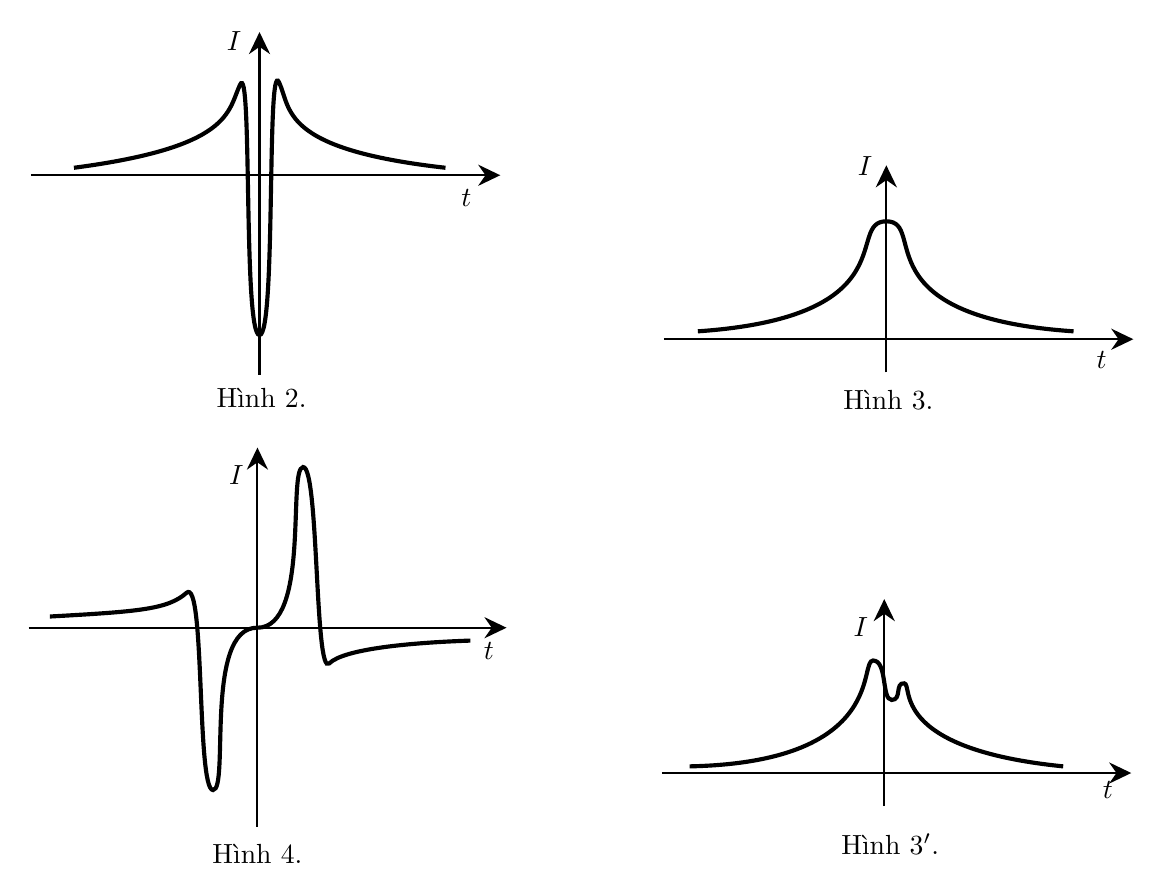
\begin{tikzpicture}[x=0.75pt,y=0.75pt,yscale=-1,xscale=1]
%uncomment if require: \path (0,428); %set diagram left start at 0, and has height of 428

%Straight Lines [id:da7208994211679127] 
\draw    (69,76) -- (292.2,76) ;
\draw [shift={(295.2,76)}, rotate = 180] [fill={rgb, 255:red, 0; green, 0; blue, 0 }  ][line width=0.08]  [draw opacity=0] (10.72,-5.15) -- (0,0) -- (10.72,5.15) -- (7.12,0) -- cycle    ;
%Straight Lines [id:da5654504449015016] 
\draw    (179.2,172) -- (179.2,10) ;
\draw [shift={(179.2,7)}, rotate = 450] [fill={rgb, 255:red, 0; green, 0; blue, 0 }  ][line width=0.08]  [draw opacity=0] (10.72,-5.15) -- (0,0) -- (10.72,5.15) -- (7.12,0) -- cycle    ;
%Curve Lines [id:da46762995420986675] 
\draw [line width=1.5]    (89.8,72.4) .. controls (165.8,62.4) and (163.8,45.4) .. (169.8,32.4) .. controls (175.8,19.4) and (171.2,153) .. (179.2,153) .. controls (187.2,153) and (182.6,18.4) .. (188.6,31.2) .. controls (194.6,44) and (188.8,63.4) .. (268.8,72.4) ;
%Straight Lines [id:da22174213812764432] 
\draw    (374,155) -- (597.2,155) ;
\draw [shift={(600.2,155)}, rotate = 180] [fill={rgb, 255:red, 0; green, 0; blue, 0 }  ][line width=0.08]  [draw opacity=0] (10.72,-5.15) -- (0,0) -- (10.72,5.15) -- (7.12,0) -- cycle    ;
%Straight Lines [id:da23004406205747574] 
\draw    (481.2,171) -- (481.2,74.2) ;
\draw [shift={(481.2,71.2)}, rotate = 450] [fill={rgb, 255:red, 0; green, 0; blue, 0 }  ][line width=0.08]  [draw opacity=0] (10.72,-5.15) -- (0,0) -- (10.72,5.15) -- (7.12,0) -- cycle    ;
%Curve Lines [id:da5364995652202349] 
\draw [line width=1.5]    (390.4,151.2) .. controls (492.4,144.2) and (461.2,98.2) .. (481.2,98.2) .. controls (501.2,98.2) and (468.4,144.2) .. (571.4,151.2) ;
%Straight Lines [id:da5806853953321698] 
\draw    (68,294) -- (295.2,294) ;
\draw [shift={(298.2,294)}, rotate = 180] [fill={rgb, 255:red, 0; green, 0; blue, 0 }  ][line width=0.08]  [draw opacity=0] (10.72,-5.15) -- (0,0) -- (10.72,5.15) -- (7.12,0) -- cycle    ;
%Straight Lines [id:da8152094843359954] 
\draw    (178.2,390) -- (178.2,210.2) ;
\draw [shift={(178.2,207.2)}, rotate = 450] [fill={rgb, 255:red, 0; green, 0; blue, 0 }  ][line width=0.08]  [draw opacity=0] (10.72,-5.15) -- (0,0) -- (10.72,5.15) -- (7.12,0) -- cycle    ;
%Curve Lines [id:da9565713037584695] 
\draw [line width=1.5]    (78.2,288.6) .. controls (121,286.2) and (135,285.2) .. (144,277.2) .. controls (153,269.2) and (148.8,372.2) .. (156.8,372.2) .. controls (164.8,372.2) and (152.4,293.8) .. (178.1,294) .. controls (203.8,294.2) and (192.6,217) .. (200.2,216.6) .. controls (207.8,216.2) and (205.8,318.2) .. (212.8,311.2) .. controls (219.8,304.2) and (251.6,301.2) .. (280.8,300.2) ;
%Straight Lines [id:da3784584126897128] 
\draw    (373,364) -- (596.2,364) ;
\draw [shift={(599.2,364)}, rotate = 180] [fill={rgb, 255:red, 0; green, 0; blue, 0 }  ][line width=0.08]  [draw opacity=0] (10.72,-5.15) -- (0,0) -- (10.72,5.15) -- (7.12,0) -- cycle    ;
%Straight Lines [id:da3421557860359772] 
\draw    (480.2,380) -- (480.2,283.2) ;
\draw [shift={(480.2,280.2)}, rotate = 450] [fill={rgb, 255:red, 0; green, 0; blue, 0 }  ][line width=0.08]  [draw opacity=0] (10.72,-5.15) -- (0,0) -- (10.72,5.15) -- (7.12,0) -- cycle    ;
%Curve Lines [id:da0692355813450043] 
\draw [line width=1.5]    (386.4,360.8) .. controls (438.24,359.71) and (457.78,344.75) .. (465.93,331.31) .. controls (472.79,320.02) and (471.6,309.8) .. (474.8,309.8) .. controls (481.8,309.8) and (478.8,328.8) .. (483.8,328.8) .. controls (488.8,328.8) and (485.2,320.4) .. (489.8,320.8) .. controls (494.4,321.2) and (481.4,352.2) .. (566.4,360.8) ;


% Text Node
\draw (162,5.4) node [anchor=north west][inner sep=0.75pt]    {$I$};
% Text Node
\draw (466,65.4) node [anchor=north west][inner sep=0.75pt]    {$I$};
% Text Node
\draw (163,214.4) node [anchor=north west][inner sep=0.75pt]    {$I$};
% Text Node
\draw (464,287.4) node [anchor=north west][inner sep=0.75pt]    {$I$};
% Text Node
\draw (275,81.4) node [anchor=north west][inner sep=0.75pt]    {$t$};
% Text Node
\draw (581,159.4) node [anchor=north west][inner sep=0.75pt]    {$t$};
% Text Node
\draw (285.8,299.6) node [anchor=north west][inner sep=0.75pt]    {$t$};
% Text Node
\draw (584,366.4) node [anchor=north west][inner sep=0.75pt]    {$t$};
% Text Node
\draw (157,177) node [anchor=north west][inner sep=0.75pt]   [align=left] {Hình $2$.};
% Text Node
\draw (459,178) node [anchor=north west][inner sep=0.75pt]   [align=left] {Hình $3$.};
% Text Node
\draw (155,397) node [anchor=north west][inner sep=0.75pt]   [align=left] {Hình $4$.};
% Text Node
\draw (458,391.8) node [anchor=north west][inner sep=0.75pt]   [align=left] {Hình $3'$.};


\end{tikzpicture}
\end{center}


\end{enumerate}
\item Đầu tiên cần lưu ý rằng một phần động năng của lưỡng cực sẽ được chuyển thành năng lượng từ trường của vòng dây do dòng điện cảm ứng gây ra $(W_L = \dfrac{LI^2}{2})$ và nhiệt năng do vòng dây tỏa ra môi trường $(\dd Q = I^2 R\cdot \dd t)$. Độ tự cảm của vòng dây trong trường hợp này là $L \approx 10^{-5} ~\mathrm{H}$ và điện trở tương ứng $R= \dfrac{2\rho a}{r^2} = 0,08 ~\Omega$. Với $x\gg r$ năng lượng mất do tự cảm tương đương với năng lượng mất do nhiệt năng. Năng lượng tự cảm chỉ đáng kể với $x \leq r$ khi từ thông thay đổi nhanh, do đó nên mô hình tính toán không kể đến năng lượng mất mát do tự cảm sẽ cho kết quả là một dòng điện vượt quá $I_{\max}^{S}$, điều này là vô lí vì điện trở của dây không thể làm tăng dòng điện. Suất điện động cảm ứng ngoài (xem $1)$) được tính bởi biểu thức
  \[U_E \approx \dfrac{\mu_0 M}{2} \dfrac{a}{(a^2 + x^2)^{3/2}}\dfrac{\dd x}{\dd t}.\]

Do đó, từ trường của dòng điện cảm ứng khi từ tích ở khoảng cách $x$ từ vòng dây (chúng ta giả sử $x<0$ khi từ tích tiến tới vòng dây và $x>0$ sau khi từ tích đã xuyên qua nó) và chuyển động với vận tốc $v$ là:
    \[ x =\dfrac{|U_E|}{R} = \dfrac{\mu_0 M}{2R} \dfrac{a^2}{(a^2 + x^2)^{3/2}}v(x).\]

Với các thông số của vòng dây đã được cung cấp, ta tính được:
   \[R \approx \dfrac{1}{125} \dfrac{Lv_0}{2r} \approx 8\dfrac{Lv_0}{a}, \]

do đó, chúng ta có đủ lí do để kết luận rằng:
   \[ \dfrac{Lv_0}{a} \ll R\ll\dfrac{Lv_0}{2r}.\]

Do đó, đồ thị trên Hình $3$ gần như tương ứng với sự phụ thuộc của dòng điện tự cảm theo thời gian và chúng ta có thể sử dụng hàm số đã thu được cho dòng điện như một xấp xỉ gần đúng cho bất kể khoảng thời gian nào. Dùng xấp xỉ này, công suất tỏa nhiệt tức thời của vòng dây là:
   \[P= I^2 R= \dfrac{(\mu_0 M)^2}{4R} \dfrac{a^4}{(a^2 + x^2)^3}v^2(x).\]

Trong trường hợp này, chúng ta cũng phải giả sử gia tốc của đơn cực từ là nhỏ như những phần trước (xem $2)$). Do đó, tổng nhiệt lượng tỏa ra trên vòng dây xấp xỉ:
    \[Q = \int_{- \infty}^{+\infty} P \dd t \approx \dfrac{(\mu_0 M)^2 v_0}{4R} \int_{- \infty}^{+\infty} \dfrac{a^4}{(a^2+x^2)^3}\dd x.\]

Vì $x = a \cdot \cot \alpha $, chúng ta có $\dd x = a \sin^{-2} \alpha \dd \alpha $, và
     \[ Q \approx \dfrac{(\mu_0 M)^2 v_0}{4Ra} \int_{0}^{\pi} \sin^4 \alpha \dd \alpha = \dfrac{3\pi (\mu_0 M)^2v_0}{32Ra} .\]

Bây giờ, sử dụng định luật bảo toàn năng lượng, ta có:
    \[ \dfrac{mv_{\min}^2 }{2} \approx \dfrac{mv_0^2}{2} - Q \Rightarrow v_0^2 - v_{\min}^2 = \dfrac{2Q}{m} \approx \dfrac{3\pi (\mu_0 M)^2 v_0}{16mRa}.\]

Vì độ thay đổi vận tốc là nhỏ, chúng ta thu được:
  \[\Delta v \approx \dfrac{v_0^2 - v_{\min}^2}{2v_0} \approx \dfrac{3\pi (\mu_0 M)^2 v_0}{32mRa} \approx 6 \cdot 10^{-6} ~\mathrm{m/s}.\]

\textbf{Lưu ý.} Ở câu hỏi $3)$ và $4)$, sự vắng mặt của năng lượng từ trường không gây ra sự thay đổi đáng kể cho kết quả cuối cùng. Do đó, tất cả thí sinh đều được cho đủ điểm kể cả không tính tới năng lượng từ trường.

\begin{center}
     \textbf{Phần II}
\end{center}
\begin{enumerate}[1)]
\item Chú ý rằng, chuyển động của một điện tích $q$ có khối lượng $m$ trong trường của một dyon cố định sẽ bảo toàn tổng động năng của điện tích và thế năng tương tác của điện tích và dyon. Công sinh ra bởi thành phần từ trường của lực Lorentz $\ot{F_M} = q \left[\ot{v}\times \ot{B} \right]$ bằng không và công của thành phần lực điện $\ot{F_E} = q\ot{E} $ có thể được tính thông qua hiệu thế năng tĩnh điện $U= \dfrac{1}{4\pi \varepsilon_0} \dfrac{qQ}{r}$ ($r$ là khoảng cách từ điện tích đến dyon). Do đó:
  \[\dfrac{mv^2}{2} + \dfrac{1}{4\pi \varepsilon_0}\dfrac{qQ}{r} = \const.\]

Do đó, nếu vận tốc của hạt là không đổi, khoảng cách của hạt đến dyon cũng phải không đổi. Điều này gợi ý rằng dyon phải nằm trên trục đối xứng của quỹ đạo tròn của hạt (xem hình vẽ).
 \begin{center}


\tikzset{every picture/.style={line width=0.75pt}} %set default line width to 0.75pt        

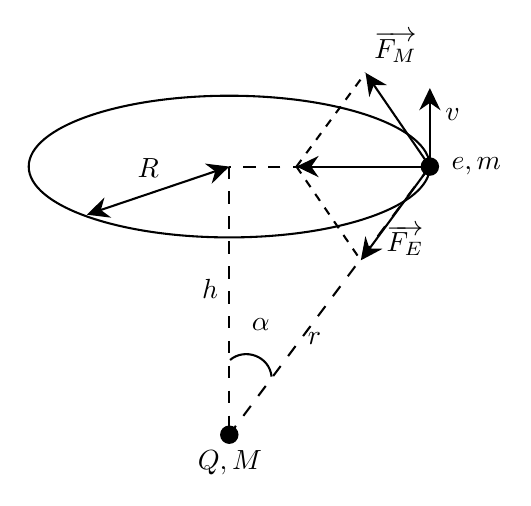
\begin{tikzpicture}[x=0.75pt,y=0.75pt,yscale=-1,xscale=1]
%uncomment if require: \path (0,300); %set diagram left start at 0, and has height of 300

%Shape: Ellipse [id:dp3248654622660052] 
\draw   (205,69.82) .. controls (205,50.96) and (248.26,35.68) .. (301.63,35.68) .. controls (355,35.68) and (398.27,50.96) .. (398.27,69.82) .. controls (398.27,88.67) and (355,103.95) .. (301.63,103.95) .. controls (248.26,103.95) and (205,88.67) .. (205,69.82) -- cycle ;
%Straight Lines [id:da14493074136253026] 
\draw  [dash pattern={on 4.5pt off 4.5pt}]  (398.27,69.82) -- (301.63,69.82) ;
%Shape: Ellipse [id:dp3345662521138948] 
\draw  [fill={rgb, 255:red, 0; green, 0; blue, 0 }  ,fill opacity=1 ] (394.34,69.82) .. controls (394.34,67.65) and (396.1,65.88) .. (398.27,65.88) .. controls (400.44,65.88) and (402.2,67.65) .. (402.2,69.82) .. controls (402.2,71.99) and (400.44,73.75) .. (398.27,73.75) .. controls (396.1,73.75) and (394.34,71.99) .. (394.34,69.82) -- cycle ;
%Straight Lines [id:da15849439435830615] 
\draw    (398.27,69.82) -- (398.27,35) ;
\draw [shift={(398.27,32)}, rotate = 450] [fill={rgb, 255:red, 0; green, 0; blue, 0 }  ][line width=0.08]  [draw opacity=0] (10.72,-5.15) -- (0,0) -- (10.72,5.15) -- (7.12,0) -- cycle    ;
%Shape: Ellipse [id:dp18197671493371637] 
\draw  [fill={rgb, 255:red, 0; green, 0; blue, 0 }  ,fill opacity=1 ] (297.7,199) .. controls (297.7,196.83) and (299.46,195.07) .. (301.63,195.07) .. controls (303.81,195.07) and (305.57,196.83) .. (305.57,199) .. controls (305.57,201.17) and (303.81,202.93) .. (301.63,202.93) .. controls (299.46,202.93) and (297.7,201.17) .. (297.7,199) -- cycle ;
%Straight Lines [id:da212894104663359] 
\draw  [dash pattern={on 4.5pt off 4.5pt}]  (301.63,69.82) -- (301.63,199) ;
%Straight Lines [id:da12179005482825844] 
\draw  [dash pattern={on 4.5pt off 4.5pt}]  (398.27,69.82) -- (301.63,199) ;
%Straight Lines [id:da2525089276202863] 
\draw    (235.84,92.04) -- (298.79,70.78) ;
\draw [shift={(301.63,69.82)}, rotate = 521.3399999999999] [fill={rgb, 255:red, 0; green, 0; blue, 0 }  ][line width=0.08]  [draw opacity=0] (10.72,-5.15) -- (0,0) -- (10.72,5.15) -- (7.12,0) -- cycle    ;
\draw [shift={(233,93)}, rotate = 341.34] [fill={rgb, 255:red, 0; green, 0; blue, 0 }  ][line width=0.08]  [draw opacity=0] (10.72,-5.15) -- (0,0) -- (10.72,5.15) -- (7.12,0) -- cycle    ;
%Straight Lines [id:da3131311012561828] 
\draw    (398.27,69.82) -- (337,69.82) ;
\draw [shift={(334,69.82)}, rotate = 360] [fill={rgb, 255:red, 0; green, 0; blue, 0 }  ][line width=0.08]  [draw opacity=0] (10.72,-5.15) -- (0,0) -- (10.72,5.15) -- (7.12,0) -- cycle    ;
%Straight Lines [id:da8584123604483767] 
\draw    (398.27,69.82) -- (368.96,27.11) ;
\draw [shift={(367.27,24.63)}, rotate = 415.55] [fill={rgb, 255:red, 0; green, 0; blue, 0 }  ][line width=0.08]  [draw opacity=0] (10.72,-5.15) -- (0,0) -- (10.72,5.15) -- (7.12,0) -- cycle    ;
%Straight Lines [id:da25928232517915606] 
\draw  [dash pattern={on 3pt off 3pt on 3pt off 3pt}]  (334,69.82) -- (367.27,24.63) ;
%Straight Lines [id:da02968211389413944] 
\draw    (366.78,112.58) -- (398.27,69.82) ;
\draw [shift={(365,115)}, rotate = 306.36] [fill={rgb, 255:red, 0; green, 0; blue, 0 }  ][line width=0.08]  [draw opacity=0] (10.72,-5.15) -- (0,0) -- (10.72,5.15) -- (7.12,0) -- cycle    ;
%Straight Lines [id:da7966932719816191] 
\draw  [dash pattern={on 3pt off 3pt on 3pt off 3pt}]  (334,69.82) -- (365,115) ;
%Curve Lines [id:da44632086073280663] 
\draw    (302,163) .. controls (309,157) and (321,161) .. (322,171) ;


% Text Node
\draw (404.2,40.4) node [anchor=north west][inner sep=0.75pt]    {$\ot{v}$};
% Text Node
\draw (407.2,64.22) node [anchor=north west][inner sep=0.75pt]    {$e,m$};
% Text Node
\draw (256,64.4) node [anchor=north west][inner sep=0.75pt]    {$R$};
% Text Node
\draw (285,205.4) node [anchor=north west][inner sep=0.75pt]    {$Q,M$};
% Text Node
\draw (287,122.4) node [anchor=north west][inner sep=0.75pt]    {$h$};
% Text Node
\draw (338,148.4) node [anchor=north west][inner sep=0.75pt]    {$r$};
% Text Node
\draw (376,96.4) node [anchor=north west][inner sep=0.75pt]    {$\overrightarrow{F_{E}}$};
% Text Node
\draw (370,3.4) node [anchor=north west][inner sep=0.75pt]    {$\overrightarrow{F_{M}}$};
% Text Node
\draw (311,141.4) node [anchor=north west][inner sep=0.75pt]    {$\alpha $};


\end{tikzpicture}
\end{center}
Lực tác dụng lên hạt:
   \[\ot{F} = q\ot{E} + q \left[\ot{v}\times \ot{B}\right] \]
phải hướng vào tâm quỹ đạo chuyển động. Bây giờ, chúng ta có thể khẳng định rằng, một quỹ đạo như thế chỉ thỏa mãn với các hạt mang điện tích âm $q<0$ để sao cho thành phần từ và thành phần điện của lực Lorentz có thể cân bằng lẫn nhau và hợp lực của chúng chỉ nằm trong mặt phẳng quỹ đạo của hạt:
  \[ \dfrac{1}{4\pi \varepsilon_0} \dfrac{|q|Q}{r^2} \cos \alpha = \dfrac{\mu_0}{4\pi} \dfrac{|q|M}{r^2}v \sin \alpha \Rightarrow \tan \alpha = \dfrac{c^2 Q}{vM}.\]

Bán kính $r$ có thể được xác định thông qua phương trình về gia tốc hướng tâm,
  \[ m \dfrac{v^2}{r \sin \alpha} = |q| \left( \dfrac{Q}{4\pi \varepsilon_0 r^2} \sin \alpha+ \dfrac{\mu_0 Mv}{4\pi r^2} \cos \alpha\right),\]
dẫn đến
  \[r = \dfrac{1}{4\pi\varepsilon_0} \dfrac{|q|Q}{mv^2}.\]

Có một tính chất hết sức thú vị là biểu thức này không hề chứa $M$: khoảng cách từ một hạt điện tích chuyển động tròn trong điện trường và từ trường của một dyon đến dyon hoàn toàn trùng với bán kính quỹ đạo của nó khi chuyển động quanh dyon với sự vắng mặt của từ trường (chỉ có điện trường của dyon sinh lực). Tuy nhiên, từ trường của dyon đã làm dịch mặt phẳng chuyển động của điện tích, do đó dyon không còn nằm trên mặt phẳng đó nữa.
 \item Theo phân tích ở trên, bán kính quỹ đạo tròn là:
 \[R = r \cdot \sin \alpha = \dfrac{1}{4\pi \varepsilon_0}\dfrac{|q|Q^2c^2}{mv^2 \sqrt{c^4 Q^2 +v^2 M^2}},\]

nằm ở một mặt phẳng cách xa dyon một khoảng:
  \[h = r \cdot \cos \alpha = \dfrac{1}{4\pi\varepsilon_0} \dfrac{|q|QM}{mv \sqrt{c^4 Q^2 + v^2 M^2}}, \]
và dyon nằm trên trục đối xứng của quỹ đạo này. Quỹ đạo có góc nửa đỉnh $\alpha = \arctan \left(\dfrac{c^2Q}{vM}\right)$ từ vị trí của dyon. Với các thông số trên, chúng ta hoàn toàn xác định được quỹ đạo của hạt.
  \item Dễ thấy, tích phân vô hướng của chuyển động sẽ cho ta tổng năng lượng của hạt:
  \[E \equiv \dfrac{mv^2}{2} + \dfrac{1}{4\pi \varepsilon_0}\dfrac{qQ}{r}.\]

Tích phân có hướng của chuyển động chắc chắn sẽ liên quan đến moment động lượng $\ot{L} = m \left[\ot{r}\times \ot{v}\right]$, đại lượng sẽ bảo toàn nếu điện tích chuyển động quanh một dyon cố định có $M=0$. Sự thay đổi của moment động lượng của điện tích trong quá trình chuyển động chỉ do thành phần từ của lực Lorentz gây ra (vì moment lực của lực điện triệt tiêu nhau):
   \[  \dfrac{\dd \ot{L}}{\dd t} = \left[\ot{r} \times \ot{F_M} \right] = \dfrac{\mu_0 M|q|}{4 \pi r^3} \left[\ot{r}\times \left[ \ot{v} \times \ot{r}\right]\right]= -\dfrac{\mu_0 M|q|}{4\pi} \left\{\dfrac{\ot{v}}{r} - \dfrac{(\ot{v}\ot{r})\ot{r}}{r^3}\right\}.\]
Vì
  \[\ot{v} = \dfrac{\dd \ot{r}}{\dd t} \,\text{ và }\, \dfrac{\left(\ot{v}\ot{r} \right)}{r}  = \dfrac{vr\cos\left(\ot{v},\ot{r}\right)}{r}= v\cos \left(\ot{v},\ot{r}\right) = v_r = \dfrac{\dd r}{\dd t},\]
chúng ta thu được:
  \[\dfrac{\ot{v}}{r} - \dfrac{\left(\ot{v}\ot{r}\right)\ot{r}}{r^3} = \dfrac{r\left(\dfrac{\dd \ot{r}}{\dd t}\right)}{r^2} - \dfrac{\left(\dfrac{\dd r}{\dd t}\right) \ot{r}}{r^2} = \dfrac{\dd}{\dd t} \left(\dfrac{\ot{r}}{r}\right).\]
Do đó:
  \[\dfrac{\dd}{\dd t}\left(\ot{L} + \dfrac{\mu_0 M |q|}{4\pi} \dfrac{\ot{r}}{r} \right) = 0.\]

Nên vector 
  \[ \ot{J} \equiv \ot{L} + \dfrac{\mu_0 M|q|}{4 \pi} \dfrac{\ot{r}}{r},\]

là bảo toàn đối với một điện tích chuyển động trong điện từ trường của dyon! Tính $E$ và $\ot{J}$ (theo tính đối xứng, $\ot{J}$ hướng dọc theo trục đối xứng của quỹ đạo) theo các thông số ta thu được cho $r$ và $\alpha$ ta có: 
  \[E = - \dfrac{mv^2}{2} \, \text{ và } \, \ot{J} = \dfrac{\mu_0 |q|}{4\pi v}\sqrt{c^4 Q^2 + v^2 M^2} \cdot \ot{n},\]
ở đây vector $\ot{n}$ hướng từ dyon đến tâm của quỹ đạo chuyển động.\\

\textbf{Lưu ý:} Điện từ trường là một loại vật chất đặc biệt mang theo cả năng lượng và động lượng (năng lượng và động lượng của nó tuân theo vector Poynting $\ot{S}= c\cdot \ot{S_p} = \dfrac{1}{\mu_0}\left[\ot{E} \times \ot{B}\right]$), và do đó, mang theo cả moment động lượng. Moment động lượng của một hệ khép kín phải được bảo toàn, trong trường hợp của chúng ta, đại lượng bảo toàn này bao gồm moment động lượng của cả điện tích và của cả từ trường trong hệ quy chiếu của dyon (vì ở hệ quy chiếu khác $\ot{S_p} \neq 0 !$). Do đó thành phần thứ hai của $\ot{J}$ chính là moment động lượng của trường điện từ và do đó, $\ot{J}$ là moment động lượng tổng cộng của hệ bao gồm dyon, điện tích và điện từ trường.
\end{enumerate}
\begin{center}
  \textbf{Phần III}
\end{center}
\begin{enumerate}[1)]
   \item Theo các phần trên, chúng ta đã biết chuyển động của một điện tích trong từ trường của một đơn cực từ sẽ bảo toàn động năng $E= \dfrac{mv^2}{2}$ và vector 
      $$\ot{J} \equiv \ot{L} - \dfrac{\mu_0 Mq}{4\pi} \dfrac{\ot{r}}{r}.$$
Chúng ta sử dụng hệ tọa độ như trong hình vẽ. 
\begin{center}


\tikzset{every picture/.style={line width=0.75pt}} %set default line width to 0.75pt        

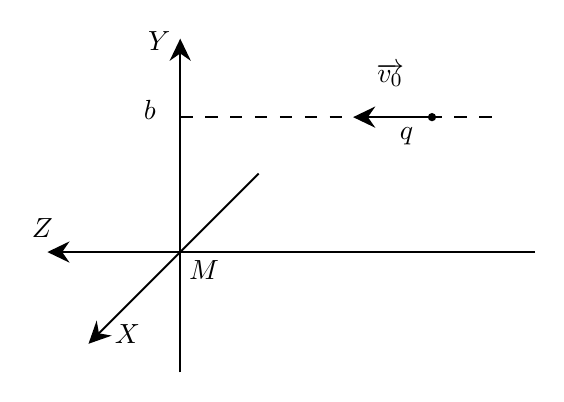
\begin{tikzpicture}[x=0.75pt,y=0.75pt,yscale=-1,xscale=1]
%uncomment if require: \path (0,300); %set diagram left start at 0, and has height of 300

%Straight Lines [id:da06648805170596872] 
\draw    (396,143) -- (164,143) ;
\draw [shift={(161,143)}, rotate = 360] [fill={rgb, 255:red, 0; green, 0; blue, 0 }  ][line width=0.08]  [draw opacity=0] (10.72,-5.15) -- (0,0) -- (10.72,5.15) -- (7.12,0) -- cycle    ;
%Straight Lines [id:da855834463364245] 
\draw    (225,201) -- (225,43.2) ;
\draw [shift={(225,40.2)}, rotate = 450] [fill={rgb, 255:red, 0; green, 0; blue, 0 }  ][line width=0.08]  [draw opacity=0] (10.72,-5.15) -- (0,0) -- (10.72,5.15) -- (7.12,0) -- cycle    ;
%Straight Lines [id:da4049918268561159] 
\draw    (262.8,105.2) -- (182.92,185.08) ;
\draw [shift={(180.8,187.2)}, rotate = 315] [fill={rgb, 255:red, 0; green, 0; blue, 0 }  ][line width=0.08]  [draw opacity=0] (10.72,-5.15) -- (0,0) -- (10.72,5.15) -- (7.12,0) -- cycle    ;
%Straight Lines [id:da2606476536092206] 
\draw  [dash pattern={on 4.5pt off 4.5pt}]  (225,78) -- (377,78) ;
%Straight Lines [id:da32259151033194566] 
\draw    (346.3,78) -- (311.3,78) ;
\draw [shift={(308.3,78)}, rotate = 360] [fill={rgb, 255:red, 0; green, 0; blue, 0 }  ][line width=0.08]  [draw opacity=0] (10.72,-5.15) -- (0,0) -- (10.72,5.15) -- (7.12,0) -- cycle    ;
%Shape: Circle [id:dp41190422982989827] 
\draw  [fill={rgb, 255:red, 0; green, 0; blue, 0 }  ,fill opacity=1 ] (344.85,78) .. controls (344.85,77.2) and (345.5,76.55) .. (346.3,76.55) .. controls (347.1,76.55) and (347.75,77.2) .. (347.75,78) .. controls (347.75,78.8) and (347.1,79.45) .. (346.3,79.45) .. controls (345.5,79.45) and (344.85,78.8) .. (344.85,78) -- cycle ;


% Text Node
\draw (227.8,145.6) node [anchor=north west][inner sep=0.75pt]    {$M$};
% Text Node
\draw (192,176.4) node [anchor=north west][inner sep=0.75pt]    {$X$};
% Text Node
\draw (152,125.4) node [anchor=north west][inner sep=0.75pt]    {$Z$};
% Text Node
\draw (208,35.4) node [anchor=north west][inner sep=0.75pt]    {$Y$};
% Text Node
\draw (206,68.4) node [anchor=north west][inner sep=0.75pt]    {$b$};
% Text Node
\draw (318,50.4) node [anchor=north west][inner sep=0.75pt]    {$\overrightarrow{v_{0}}$};
% Text Node
\draw (329.3,81.4) node [anchor=north west][inner sep=0.75pt]    {$q$};


\end{tikzpicture}
\end{center}
Khi điện tích ở cách xa đơn cực từ,
   \[\left|\ot{v}\right| \equiv \ot{v_0}, \ot{v} = v_0 \ot{e_z} , \ot{r} = b\ot{e_y} - r_z \ot{e_z}, \, \text{ và }\, r = \sqrt{b^2 +r_z^2},\]
ở đây $r \approx r_z \gg b$. Và sau đó:
   \[\ot{J} \equiv m \left[\ot{r}\times \ot{v}\right] - \dfrac{\mu_0 Mq}{4\pi} \dfrac{\ot{r}}{r} \equiv mv_0 b \ot{e_x} + \dfrac{\mu_0 Mq}{4\pi}\ot{e_z}.\]

Sau khi tán xạ trên đơn cực từ và đi ra rất xa, điện tích sẽ di chuyển trên một đường thẳng với vận tốc $v'$. Rõ ràng rằng $v'=v_0$ do năng lượng $E$ được bảo toàn.
\item Đặt $\ot{n}$ là vector chỉ phương của $\ot{v'}$ và $\ot{b'}$ là vector hướng từ đơn cực từ đến điểm gần nhất trên quỹ đạo của điện tích sau khi tán xạ. Do đó, vector chỉ hướng của điện tích, khi nó ở khoảng cách $r$ từ đơn cực từ sẽ là:
$$\ot{r} = \ot{b'} + \ot{n}\sqrt{r^2 - b'^2}.$$
Theo cách chọn hệ quy chiếu, vector $\ot{n}$ sẽ song song với mặt phẳng $(yz)$, ta có thể viết:
$$\ot{n} = \pm \sin \theta \ot{e_y} + \cos \theta \ot{e_z},$$
ở đây $\theta$ là góc hợp bởi $\ot{v'}$ và $\ot{v_0}$. Chúng ta cũng dễ thấy $\ot{b'} \perp \ot{n}$. Sử dụng phương trình bảo toàn ta thu được:
    \[ \dfrac{\left[\ot{r} \times \ot{v'}\right]}{v_0} - \dfrac{\mu_0 Mq}{4 \pi m v_0 } \dfrac{\ot{r}}{r} = \left[\ot{b'}\times \ot{n}\right] - \dfrac{\mu_0 Mq}{4\pi m v_0}\ot{n} = b \ot{e_x} + \dfrac{\mu_0 Mq}{4\pi m v_0}\ot{e_z}.\]

Để đơn giản hóa biểu thức chúng ta đặt biến $\dfrac{\mu_0Mq}{4\pi mv_0} = \beta$ và tính tích chéo của biểu thức trên với $\ot{n}$, dẫn tới: 
$$\ot{b'} = b\left[\ot{n}\times \ot{e_x}\right] + \beta \left[\ot{n} \times \ot{e_z}\right].$$
Thay thế biểu thức của $\ot{n}$ chúng ta thu được từ phương trình này, dẫn tới:
   \[\ot{b'} = \pm \beta \sin \theta \ot{e_x} + b \cos \theta\ot{e_y} \mp b \sin \theta \ot{e_z}.\]
Do đó, khoảng cách đến mặt phẳng chuyển động của điện tích sau khi tán xạ là:
  \[ d= |d_x| = \left|\beta \sin \theta \right|.\]

Do đó, chúng ta thu được hai giá trị thỏa mãn của góc tán xạ:
   \[ \theta_1 = \arcsin \left(\dfrac{4\pi m v_0 d}{\mu_0 |Mq|}\right) \quad \text{và} \quad \theta_2 = \pi - \arcsin \left(\dfrac{4\pi m v_0 d}{\mu_0 |Mq|}\right).\]

Chúng ta có thể thấy rằng, bài toán chỉ đúng với $d \leq \dfrac{\mu_0 |Mq|}{4\pi m v_0}$ (tất cả các giá trị thỏa mãn của $d$ đều nằm trong vùng này).
\item Đầu tiên, chúng ta có độ lớn của $\ot{b'}$
    \[ b' = \sqrt{b^2 + \beta^2 \sin^2 \theta} = \sqrt{b^2 + d^2}.\]
Tiếp đó, khi bình phương hai vế của phương trình:
   \[ \left[\ot{b'} \times \ot{n}\right] - \beta \ot{n} = b\ot{e_x} + \beta\ot{e_z},\]
cùng với việc đã biết $\left[\ot{b'}\times \ot{n}\right]$ vuông góc với $\ot{n}$, và $\ot{e_x}$ vuông góc với $\ot{e_y}$ nên
  \[\left[\ot{b'} \times \ot{n} \right]^2 + \beta^2 = b^2 + \beta^2.\]

Vì $\ot{b'}$ và $\ot{n}$ cũng vuông góc nên $\left[\ot{b'} \times \ot{n}\right]^2 = b'^2.$ Và cuối cùng, $b'=b$! Kết quả này càng củng cố thêm giới hạn của $d$: từ hai phương trình trên ta thu được $d=0$. Cùng lúc đó, ta có $\sin \theta =0$ nên $\theta_1 =0$ hoặc $\theta_2 = \pi$. Trên thực tế, trường hợp $\theta =0$ chỉ xảy ra với giới hạn $b$ và $v_0$ tiến đến vô cùng. Một hiện tượng hết sức thú vị, sau khi bị tán xạ bởi đơn cực từ, điện tích đi ngược lại theo hướng của quỹ đạo cũ!
\item Chúng ta dễ dàng suy luận từ cơ học lượng tử rằng moment động lượng của hệ (điện tích $+$ đơn cực $+$ điện từ trường) theo hướng $\ot{n} = \dfrac{\ot{r}}{r} $ phải là một số nguyên lần của $\dfrac{h}{4\pi}$. Điều này dẫn tới biểu thức:
$$\dfrac{\mu_0 Mq}{4\pi} = k \cdot \dfrac{h}{4\pi} \Rightarrow qM = k\cdot \dfrac{h}{\mu_0 },$$
với $k$ là một số nguyên. Do đó, theo giả thuyết này, bất kì điện tích nào đều là một số nguyên lần của điện tích nguyên tố:
$$\dfrac{h}{\mu_0 M} = e \Rightarrow M = \dfrac{h}{\mu_0 e} \approx 3,3 \cdot 10^{-9} ~\mathrm{Cm/s}.$$
\end{enumerate}


  \end{enumerate}

  

\end{loigiai}